\documentclass[]{book}
\usepackage{lmodern}
\usepackage{amssymb,amsmath}
\usepackage{ifxetex,ifluatex}
\usepackage{fixltx2e} % provides \textsubscript
\ifnum 0\ifxetex 1\fi\ifluatex 1\fi=0 % if pdftex
  \usepackage[T1]{fontenc}
  \usepackage[utf8]{inputenc}
\else % if luatex or xelatex
  \ifxetex
    \usepackage{mathspec}
  \else
    \usepackage{fontspec}
  \fi
  \defaultfontfeatures{Ligatures=TeX,Scale=MatchLowercase}
\fi
% use upquote if available, for straight quotes in verbatim environments
\IfFileExists{upquote.sty}{\usepackage{upquote}}{}
% use microtype if available
\IfFileExists{microtype.sty}{%
\usepackage{microtype}
\UseMicrotypeSet[protrusion]{basicmath} % disable protrusion for tt fonts
}{}
\usepackage[margin=1in]{geometry}
\usepackage{hyperref}
\PassOptionsToPackage{usenames,dvipsnames}{color} % color is loaded by hyperref
\hypersetup{unicode=true,
            pdftitle={Studieren und Forschen mit dem Internet},
            pdfauthor={Peter Baumgartner, Sabine Payr},
            colorlinks=true,
            linkcolor=Maroon,
            citecolor=Blue,
            urlcolor=Blue,
            breaklinks=true}
\urlstyle{same}  % don't use monospace font for urls
\usepackage{natbib}
\bibliographystyle{apalike}
\usepackage{longtable,booktabs}
\usepackage{graphicx,grffile}
\makeatletter
\def\maxwidth{\ifdim\Gin@nat@width>\linewidth\linewidth\else\Gin@nat@width\fi}
\def\maxheight{\ifdim\Gin@nat@height>\textheight\textheight\else\Gin@nat@height\fi}
\makeatother
% Scale images if necessary, so that they will not overflow the page
% margins by default, and it is still possible to overwrite the defaults
% using explicit options in \includegraphics[width, height, ...]{}
\setkeys{Gin}{width=\maxwidth,height=\maxheight,keepaspectratio}
\IfFileExists{parskip.sty}{%
\usepackage{parskip}
}{% else
\setlength{\parindent}{0pt}
\setlength{\parskip}{6pt plus 2pt minus 1pt}
}
\setlength{\emergencystretch}{3em}  % prevent overfull lines
\providecommand{\tightlist}{%
  \setlength{\itemsep}{0pt}\setlength{\parskip}{0pt}}
\setcounter{secnumdepth}{5}
% Redefines (sub)paragraphs to behave more like sections
\ifx\paragraph\undefined\else
\let\oldparagraph\paragraph
\renewcommand{\paragraph}[1]{\oldparagraph{#1}\mbox{}}
\fi
\ifx\subparagraph\undefined\else
\let\oldsubparagraph\subparagraph
\renewcommand{\subparagraph}[1]{\oldsubparagraph{#1}\mbox{}}
\fi

%%% Use protect on footnotes to avoid problems with footnotes in titles
\let\rmarkdownfootnote\footnote%
\def\footnote{\protect\rmarkdownfootnote}

%%% Change title format to be more compact
\usepackage{titling}

% Create subtitle command for use in maketitle
\newcommand{\subtitle}[1]{
  \posttitle{
    \begin{center}\large#1\end{center}
    }
}

\setlength{\droptitle}{-2em}
  \title{Studieren und Forschen mit dem Internet}
  \pretitle{\vspace{\droptitle}\centering\huge}
  \posttitle{\par}
\subtitle{Methoden und Werkzeuge des wissenschaftlichen Arbeitens}
  \author{Peter Baumgartner, Sabine Payr}
  \preauthor{\centering\large\emph}
  \postauthor{\par}
  \predate{\centering\large\emph}
  \postdate{\par}
  \date{2017-10-14}

% my own code
\usepackage[english, ngerman]{babel}
\usepackage[Lenny]{fncychap}
% \usepackage[utf8]{inputenc}
% \usepackage{coloremoji}

% \usepackage{titlesec}
% \titlelabel{\thetitel.\enspace}
% \titleformat{\chapter}[display]
%  {\normalfont\bfseries}{}{0pt}{\Large}

% copied from https://github.com/rstudio/bookdown/edit/master/inst/examples/latex/preamble.tex

\usepackage{booktabs}
\usepackage{longtable}
% \usepackage[bf,singlelinecheck=off]{caption}

% \usepackage{Alegreya}

% \setmainfont[UprightFeatures={SmallCapsFont=AlegreyaSC-Regular}]{Alegreya}

\usepackage{amsthm}
\newtheorem{theorem}{Theorem}[chapter]
\newtheorem{lemma}{Lemma}[chapter]
\theoremstyle{definition}
\newtheorem{definition}{Definition}[chapter]
\newtheorem{corollary}{Corollary}[chapter]
\newtheorem{proposition}{Proposition}[chapter]
\theoremstyle{definition}
\newtheorem{example}{Example}[chapter]
\theoremstyle{definition}
\newtheorem{exercise}{Exercise}[chapter]
\theoremstyle{remark}
\newtheorem*{remark}{Remark}
\newtheorem*{solution}{Solution}
\begin{document}
\maketitle

{
\hypersetup{linkcolor=black}
\setcounter{tocdepth}{2}
\tableofcontents
}
\chapter*{Vorwort}\label{vorwort}
\addcontentsline{toc}{chapter}{Vorwort}

\begin{center}\href{http://www.studienverlag.at/page.cfm?vpath=buecher/buchdetail&titnr=1319}{
\includegraphics{images/cover-stufonet-min} }\end{center}

\chapter*{Einleitung}\label{einleitung}
\addcontentsline{toc}{chapter}{Einleitung}

\chapter{Konzipieren einer Arbeit}\label{konzipieren-einer-arbeit}

\begin{figure}

{\centering 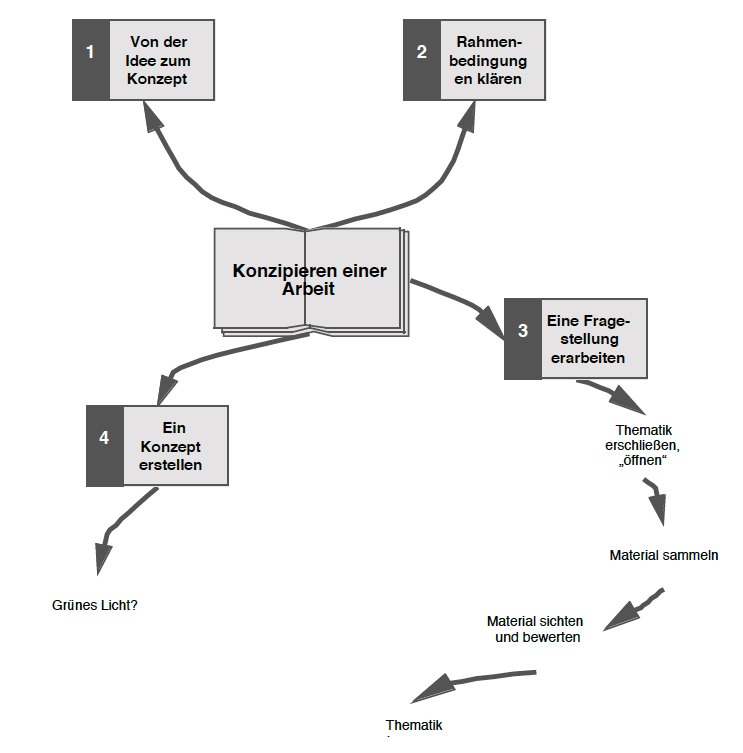
\includegraphics{images/konzipieren-min} 

}

\caption{Konzipieren (Übersicht)}\label{fig:unnamed-chunk-1}
\end{figure}

\section{Von der Idee zum Konzept}\label{von-der-idee-zum-konzept}

Am Anfang jeder Arbeit sollte ein eigenes -- wenn auch noch vages --
Interesse an einem Problem, an einem Sachgebiet stehen. Persönliches
Engagement ist der beste Start für die harte Arbeit, die vor Ihnen
liegt. Sich eine Thematik von der Betreuerin oder der Professorin bloß
zuweisen zu lassen, ohne eigenes Interesse oder zumindest einen eigenen
Gesichtspunkt einzubringen, ist zwar bequem und spart anfangs auch etwas
Zeit, kann aber leicht in eine Sackgasse führen. Wissenschaftliches
Arbeiten lässt sich nicht mit „Dienst nach Vorschrift`` abarbeiten,
umsetzen oder aussitzen, sondern braucht Motivation, Engagement und
Kreativität.

Eine erste Idee oder vages Interesse ist aber noch lange kein
bearbeitbares Thema. Das Thema muss erst mühsam daraus entwickelt
werden. Stürzt man sich gleich, bloß mit einer vagen Ausgangsüberlegung,
in die Arbeit, dann ist die Gefahr groß, dass das Thema viel zu breit
und allgemein angelegt ist: man stößt auf immer mehr interessante
Facetten, wirft immer neue Fragen auf, und weiß schließlich nicht mehr,
wo anfangen und wo aufhören. Schon die Materialsuche will kein Ende mehr
nehmen, Lesen oder Exzerpieren wird zu einer Lebensaufgabe.

Es zahlt sich daher aus, für die Phase der Konzeptentwicklung genügend
Zeit vorzusehen. Es wird kaum verlorene Zeit sein, denn erstens kann man
sich späteren unnötigen Aufwand ersparen, und zweitens ist das meiste
des hier Gesammelten und Überlegten für die Arbeit bereits verwendbar.
Selbst wenn man durch die Vorarbeiten entdeckt, dass die ursprüngliche
Idee ungeeignet ist und verworfen werden muss, so ist es immer noch
besser, jetzt nochmals neu anzufangen als vielleicht erst Monate später.

Mit diesem Kapitel möchten wir versuchen, Ihnen Tipps und Hilfen für den
Weg von der ersten Idee über die Themenfindung und -eingrenzung bis zum
Exposé der Arbeit zu geben. Leider können das nur relativ allgemeine
Vorschläge sein. Warum? Konzeptionelle Arbeit erfordert Kreativität und
lässt sich mit formalen Verhaltensregeln nicht vollständig beschreiben.
Jeder soll und muss die eigenen Vorlieben und Methoden entdecken und
nutzen. Wie diese individuellen Wege zu einem konkreten Konzept oder
Exposé aber auch aussehen mögen, irgendeine Art von methodischem
Vorgehen ist notwendig, um sich den Rahmen für eine machbare,
überschaubare Arbeit zu schaffen.

\begin{figure}

{\centering 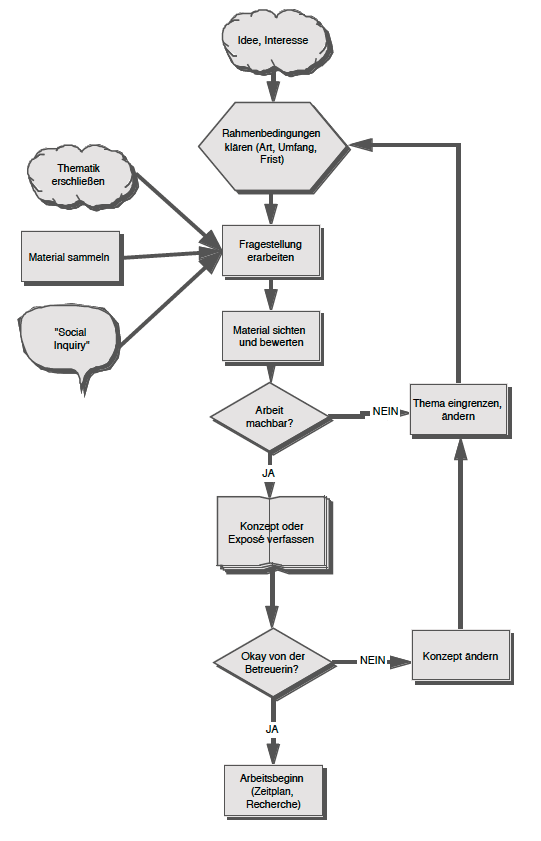
\includegraphics{images/konzipieren-von-idee-zum-arbeitsbeginn-min} 

}

\caption{Von der Idee zum Arbeitsbeginn}\label{fig:unnamed-chunk-2}
\end{figure}

\section{Rahmenbedingungen klären}\label{rahmenbedingungen-klaren}

Als Rahmenbedingungen gelten jene äußeren Faktoren, unter denen die
wissenschaftlichen Arbeiten durchgeführt werden müssen. Neben den drei
wichtigsten Faktoren Zeit, Geld und Infrastruktur können auch andere
Bedingungen (z. B. formale Vorschriften) je nach Thema Einfluss auf die
Arbeitsbedingungen haben. Die Untersuchung der äußeren
Rahmenbedingungen, unter denen die Arbeit gemacht werden muss, ist
weniger eine eigene, getrennte Phase in der Projektvorbereitung als eine
Reihe von Fragen, die man sich von Anfang an stellt und die immer wieder
bei der Entwicklung des Konzepts eine Rolle spielen.

Der wichtigste, aber auch am schwersten einzuschätzende Faktor ist die
Zeit. Vorgehensweise, Methodik und die gewählten Arbeitsschritte hängen
natürlich weitgehend vom Typus der Arbeit, dem Umfang und der
Komplexität der Fragestellung ab. Das ist ein weiterer Grund, warum es
schwierig ist, allgemeine Hilfestellungen zu geben. Doch zumindest
können für Qualifikationsarbeiten, wie sie für Studium und
wissenschaftliche Karriere verlangt werden, Richtwerte (z. B. die im
Studienplan vorgesehenen Zeiten) oder durchschnittliche Erfahrungswerte
angegeben werden. Diese Werte dienen als erste Orientierung, von denen
dann auf die entsprechenden Arbeitsphasen rückgerechnet werden kann.

Ein anderer Begrenzungsfaktor ist der bei bestimmten Arbeiten
vorgegebene Abgabetermin. Für Zeitschriftenartikel oder Kongressbeiträge
gibt es fixe Termine, aber auch für Diplomarbeiten kann es eine
festgelegte Bearbeitungsfrist geben. Hier wird man vom Endtermin
ausgehen und rückrechnen, um herauszufinden, wieviel Zeit man sich für
die einzelnen Phasen erlauben kann. Dabei sollte man unterscheiden
zwischen „Brutto`` (die Wochen, Monate \ldots{} bis zur Fertigstellung)
und „Netto`` (die tatsächlich während eines Tages, einer Woche etc. für
die Arbeit verfügbare Zeit).

Die „Nettozeit`` können Sie herausfinden, indem Sie eine Woche hindurch
über die Verwendung Ihrer Zeit Buch führen. Wenn Sie dabei realistische
Zeiten für Essen, Schlafen, Erholung, Fahrten, andere Arbeiten usw.
berücksichtigen und dazu noch Pufferzeiten für unvorhergesehene
Ereignisse mitrechnen (und nicht zu knapp), dann kommen Sie
wahrscheinlich zu einer Netto-Arbeitszeit, die wesentlich geringer ist,
als Sie angenommen hatten. Das macht aber nichts -- denn dies ist dafür
nun eine realistische Annahme. Bedenken Sie auch, dass anspruchsvolle
Arbeiten wie Lesen und Schreiben kaum „zwischendurch`` in einer
freigebliebenen Stunde möglich sind, sondern dass Sie Blöcke von
mehreren Stunden brauchen, um sich voll auf Ihre Arbeit konzentrieren zu
können (was nicht heißt, dass Sie dabei nicht kurze Entspannungspausen
einlegen sollen).

Das folgende Beispiel für einen Zeitplan orientiert sich an einer
Magister- oder Diplomarbeit, für die ca. sechs Monate zur Verfügung
stehen. Als wöchentliche Netto- Arbeitszeit wurden durchschnittlich 40
Stunden angenommen (also relativ viel!), bei fünf Arbeitstagen pro
Woche:

\subsection{Zeitplan für eine größere Arbeit (z. B.
Diplomarbeit)}\label{zeitplan-fur-eine-groere-arbeit-z.-b.-diplomarbeit}

\begin{longtable}[]{@{}lll@{}}
\caption{\textbf{\label{tab:zeitplan-gross} Zeitplan für eine größere Arbeit
(z. B. Diplomarbeit)}}\tabularnewline
\toprule
\begin{minipage}[b]{0.16\columnwidth}\raggedright\strut
Sie rechnen~\ldots{}\strut
\end{minipage} & \begin{minipage}[b]{0.35\columnwidth}\raggedright\strut
für \ldots{}\strut
\end{minipage} & \begin{minipage}[b]{0.41\columnwidth}\raggedright\strut
vorausgesetzt, dass Sie \ldots{}\strut
\end{minipage}\tabularnewline
\midrule
\endfirsthead
\toprule
\begin{minipage}[b]{0.16\columnwidth}\raggedright\strut
Sie rechnen~\ldots{}\strut
\end{minipage} & \begin{minipage}[b]{0.35\columnwidth}\raggedright\strut
für \ldots{}\strut
\end{minipage} & \begin{minipage}[b]{0.41\columnwidth}\raggedright\strut
vorausgesetzt, dass Sie \ldots{}\strut
\end{minipage}\tabularnewline
\midrule
\endhead
\begin{minipage}[t]{0.16\columnwidth}\raggedright\strut
zwei Wochen\strut
\end{minipage} & \begin{minipage}[t]{0.35\columnwidth}\raggedright\strut
erste Materialsammlung\strut
\end{minipage} & \begin{minipage}[t]{0.41\columnwidth}\raggedright\strut
bereits eine Idee haben\vspace{5mm}\strut
\end{minipage}\tabularnewline
\begin{minipage}[t]{0.16\columnwidth}\raggedright\strut
eine Woche\strut
\end{minipage} & \begin{minipage}[t]{0.35\columnwidth}\raggedright\strut
Konzepterstellung\strut
\end{minipage} & \begin{minipage}[t]{0.41\columnwidth}\raggedright\strut
danach ein Gespräch mit dem/der Betreuer/in führen\vspace{5mm}\strut
\end{minipage}\tabularnewline
\begin{minipage}[t]{0.16\columnwidth}\raggedright\strut
zwei Wochen\strut
\end{minipage} & \begin{minipage}[t]{0.35\columnwidth}\raggedright\strut
Konzeptüberarbeitung\strut
\end{minipage} & \begin{minipage}[t]{0.41\columnwidth}\raggedright\strut
das Konzept nach dem Betreuungsgespräch ändern müssen\vspace{5mm}\strut
\end{minipage}\tabularnewline
\begin{minipage}[t]{0.16\columnwidth}\raggedright\strut
drei Wochen\strut
\end{minipage} & \begin{minipage}[t]{0.35\columnwidth}\raggedright\strut
Literatursuche, -auswahl und -beschaffung\strut
\end{minipage} & \begin{minipage}[t]{0.41\columnwidth}\raggedright\strut
„grünes Licht`` bekommen haben und ca. 100 Seiten pro Tag überfliegen
können\vspace{5mm}\strut
\end{minipage}\tabularnewline
\begin{minipage}[t]{0.16\columnwidth}\raggedright\strut
neun Wochen\strut
\end{minipage} & \begin{minipage}[t]{0.35\columnwidth}\raggedright\strut
Lesen und notieren\strut
\end{minipage} & \begin{minipage}[t]{0.41\columnwidth}\raggedright\strut
ca. 50 Seiten pro Tag analytischlesen können, inkl. Notizen
machen\vspace{5mm}\strut
\end{minipage}\tabularnewline
\begin{minipage}[t]{0.16\columnwidth}\raggedright\strut
vier Wochen\strut
\end{minipage} & \begin{minipage}[t]{0.35\columnwidth}\raggedright\strut
Rohfassung schreiben\strut
\end{minipage} & \begin{minipage}[t]{0.41\columnwidth}\raggedright\strut
bei 80-100 Seiten Gesamtumfang ca. 4-5 Seiten pro Tag
schreiben\vspace{5mm}\strut
\end{minipage}\tabularnewline
\begin{minipage}[t]{0.16\columnwidth}\raggedright\strut
drei Wochen\strut
\end{minipage} & \begin{minipage}[t]{0.35\columnwidth}\raggedright\strut
Überarbeitung der Rohfassung\strut
\end{minipage} & \begin{minipage}[t]{0.41\columnwidth}\raggedright\strut
Einleitung, Schluss, Übergänge noch formulieren müssen\vspace{5mm}\strut
\end{minipage}\tabularnewline
\begin{minipage}[t]{0.16\columnwidth}\raggedright\strut
eine Woche\strut
\end{minipage} & \begin{minipage}[t]{0.35\columnwidth}\raggedright\strut
Fertigstellung\strut
\end{minipage} & \begin{minipage}[t]{0.41\columnwidth}\raggedright\strut
alle inhaltlichen Teile vollständig haben; alle bibliografischen Angaben
verfügbar haben\vspace{5mm}\strut
\end{minipage}\tabularnewline
\begin{minipage}[t]{0.16\columnwidth}\raggedright\strut
\textbf{25 Wochen}\strut
\end{minipage} & \begin{minipage}[t]{0.35\columnwidth}\raggedright\strut
\textbf{die gesamte Arbeit bis zur Abgabe}\strut
\end{minipage} & \begin{minipage}[t]{0.41\columnwidth}\raggedright\strut
\strut
\end{minipage}\tabularnewline
\bottomrule
\end{longtable}

\subsection{Zeitplan für eine
Semesterarbeit}\label{zeitplan-fur-eine-semesterarbeit}

Zum Vergleich dazu zeigen wir hier noch einen möglichen Zeitplan für
eine kleinere Arbeit (z. B. Semesterarbeit), die nebenher geschrieben
werden muss. Hier wurden als wöchentliche Arbeitszeit ca. 10 Stunden
angenommen, und als Zeitbudget zehn Wochen.

\begin{longtable}[]{@{}lll@{}}
\caption{\textbf{\label{tab:zeitplan-klein} Zeitplan für eine kleinere
Arbeit (z. B. Semesterarbeit)}}\tabularnewline
\toprule
\begin{minipage}[b]{0.14\columnwidth}\raggedright\strut
Sie rechnen~\ldots{}\strut
\end{minipage} & \begin{minipage}[b]{0.40\columnwidth}\raggedright\strut
für \ldots{}\strut
\end{minipage} & \begin{minipage}[b]{0.37\columnwidth}\raggedright\strut
Sie sollten \ldots{}\strut
\end{minipage}\tabularnewline
\midrule
\endfirsthead
\toprule
\begin{minipage}[b]{0.14\columnwidth}\raggedright\strut
Sie rechnen~\ldots{}\strut
\end{minipage} & \begin{minipage}[b]{0.40\columnwidth}\raggedright\strut
für \ldots{}\strut
\end{minipage} & \begin{minipage}[b]{0.37\columnwidth}\raggedright\strut
Sie sollten \ldots{}\strut
\end{minipage}\tabularnewline
\midrule
\endhead
\begin{minipage}[t]{0.14\columnwidth}\raggedright\strut
zwei Wochen\strut
\end{minipage} & \begin{minipage}[t]{0.40\columnwidth}\raggedright\strut
erste Materialsammlung und Konzipieren der Arbeit\strut
\end{minipage} & \begin{minipage}[t]{0.37\columnwidth}\raggedright\strut
frühzeitig das Thema und damit die Literatursuche
eingrenzen\vspace{5mm}\strut
\end{minipage}\tabularnewline
\begin{minipage}[t]{0.14\columnwidth}\raggedright\strut
eine Woche\strut
\end{minipage} & \begin{minipage}[t]{0.40\columnwidth}\raggedright\strut
ergänzende systematische Literatursuche und -beschaffung\strut
\end{minipage} & \begin{minipage}[t]{0.37\columnwidth}\raggedright\strut
sich auf rasch zugängliche Literatur beschränken und die Suche streng
zeitlich begrenzen\vspace{5mm}\strut
\end{minipage}\tabularnewline
\begin{minipage}[t]{0.14\columnwidth}\raggedright\strut
drei Wochen\strut
\end{minipage} & \begin{minipage}[t]{0.40\columnwidth}\raggedright\strut
Lesen und Notieren\strut
\end{minipage} & \begin{minipage}[t]{0.37\columnwidth}\raggedright\strut
Notizen möglichst so verfassen, dass sie im Text verwendet werden
können\vspace{5mm}\strut
\end{minipage}\tabularnewline
\begin{minipage}[t]{0.14\columnwidth}\raggedright\strut
drei Wochen\strut
\end{minipage} & \begin{minipage}[t]{0.40\columnwidth}\raggedright\strut
Rohfassung schreiben\strut
\end{minipage} & \begin{minipage}[t]{0.37\columnwidth}\raggedright\strut
bei 30 Seiten Gesamtumfang durchschnittlich 2 Seiten pro Tag
schreiben\vspace{5mm}\strut
\end{minipage}\tabularnewline
\begin{minipage}[t]{0.14\columnwidth}\raggedright\strut
eine Woche\strut
\end{minipage} & \begin{minipage}[t]{0.40\columnwidth}\raggedright\strut
Überarbeitung und Fertigstellung\strut
\end{minipage} & \begin{minipage}[t]{0.37\columnwidth}\raggedright\strut
Formvorschriften, Zitierweise usw. schon beim Schreiben
berücksichtigen\vspace{5mm}\strut
\end{minipage}\tabularnewline
\begin{minipage}[t]{0.14\columnwidth}\raggedright\strut
\textbf{zehn Wochen}\strut
\end{minipage} & \begin{minipage}[t]{0.40\columnwidth}\raggedright\strut
\textbf{die gesamte Arbeit bis zur Abgabe}\strut
\end{minipage} & \begin{minipage}[t]{0.37\columnwidth}\raggedright\strut
\strut
\end{minipage}\tabularnewline
\bottomrule
\end{longtable}

\subsection{Rahmenbedingungen
abklären}\label{rahmenbedingungen-abklaren}

\begin{longtable}[]{@{}l@{}}
\caption{\textbf{\label{tab:rahmenbedingungen} Rahmenbedingungen
klären}}\tabularnewline
\toprule
\begin{minipage}[t]{0.97\columnwidth}\raggedright\strut
\begin{itemize}
\tightlist
\item
  Wieviel Zeit steht mir für die Arbeit zur Verfügung? (Abgabetermin,
  Bearbeitungsfrist, eigene Planung) \vspace{-6mm}
\end{itemize}\strut
\end{minipage}\tabularnewline
\begin{minipage}[t]{0.97\columnwidth}\raggedright\strut
\begin{itemize}
\tightlist
\item
  Wieviel Zeit werde ich für die einzelnen Phasen benötigen, bzw.
  wieviel darf ich mir erlauben? \vspace{-6mm}
\end{itemize}\strut
\end{minipage}\tabularnewline
\begin{minipage}[t]{0.97\columnwidth}\raggedright\strut
\begin{itemize}
\tightlist
\item
  Wieviel Geld steht mir zur Verfügung, z. B. für Anschaffung von
  Literatur, Kopien, Reisen, Software, Internet-Zugang usw.?
  \vspace{-6mm}
\end{itemize}\strut
\end{minipage}\tabularnewline
\begin{minipage}[t]{0.97\columnwidth}\raggedright\strut
\begin{itemize}
\tightlist
\item
  Welche Infrastruktur steht zur Verfügung, mit welchen Beschränkungen?
  (z. B. PC-Benutzerräume -- Ausstattung, Auslastung? Bibliotheken --
  Öffnungszeiten, Urlaubssperren, Entleihfristen?) \vspace{-6mm}
\end{itemize}\strut
\end{minipage}\tabularnewline
\begin{minipage}[t]{0.97\columnwidth}\raggedright\strut
\begin{itemize}
\tightlist
\item
  Wie ist die Betreuung organisiert? (regelmäßige Treffen oder
  Sprechstunden, Terminvereinbarung, Abwesenheit \ldots{})
\end{itemize}\strut
\end{minipage}\tabularnewline
\bottomrule
\end{longtable}

Der Einfluss dieser äußeren Bedingungen auf die Themenwahl, aber auch
auf Methoden, Ansprüche, Umfang usw. kann sich in verschiedenen
Entscheidungen niederschlagen. Die nachfolgende Tabelle listet einige --
längst nicht alle -- Schwierigkeiten auf:

\begin{longtable}[]{@{}lll@{}}
\caption{\textbf{\label{tab:auswirkungen} Auswirkungen der
Rahmenbedinungen}}\tabularnewline
\toprule
\begin{minipage}[b]{0.26\columnwidth}\raggedright\strut
Sie haben z.B.\ldots{}\strut
\end{minipage} & \begin{minipage}[b]{0.30\columnwidth}\raggedright\strut
Sie entscheiden\ldots{}\strut
\end{minipage} & \begin{minipage}[b]{0.35\columnwidth}\raggedright\strut
\ldots{} und handeln (Beispiele)\strut
\end{minipage}\tabularnewline
\midrule
\endfirsthead
\toprule
\begin{minipage}[b]{0.26\columnwidth}\raggedright\strut
Sie haben z.B.\ldots{}\strut
\end{minipage} & \begin{minipage}[b]{0.30\columnwidth}\raggedright\strut
Sie entscheiden\ldots{}\strut
\end{minipage} & \begin{minipage}[b]{0.35\columnwidth}\raggedright\strut
\ldots{} und handeln (Beispiele)\strut
\end{minipage}\tabularnewline
\midrule
\endhead
\begin{minipage}[t]{0.26\columnwidth}\raggedright\strut
eine fixe Abgabefrist für die Arbeit\strut
\end{minipage} & \begin{minipage}[t]{0.30\columnwidth}\raggedright\strut
Ist das Thema in diesem Zeitrahmen machbar?\strut
\end{minipage} & \begin{minipage}[t]{0.35\columnwidth}\raggedright\strut
Thema eingrenzen, Methode ändern (z. B. nur Literaturstudie oder nur
empirische Arbeit) \vspace{5mm}\strut
\end{minipage}\tabularnewline
\begin{minipage}[t]{0.26\columnwidth}\raggedright\strut
beschränkten Internet-Zugang\strut
\end{minipage} & \begin{minipage}[t]{0.30\columnwidth}\raggedright\strut
Wann und wofür verwenden Sie das Internet, wie lässt sich die
beschränkte Zeit sinnvoll nutzen?\strut
\end{minipage} & \begin{minipage}[t]{0.35\columnwidth}\raggedright\strut
Zeit des Internet-Zugang planen (Uni, Tageszeit), Hilfsmittel kaufen (z.
B. Offline Browser) \vspace{5mm}\strut
\end{minipage}\tabularnewline
\begin{minipage}[t]{0.26\columnwidth}\raggedright\strut
beschränkten Zugang zu PCs, Druckern etc.\strut
\end{minipage} & \begin{minipage}[t]{0.30\columnwidth}\raggedright\strut
Wann und wie wird dieser Zugang am effektivsten genutzt? Lässt sich der
Zustand ändern?\strut
\end{minipage} & \begin{minipage}[t]{0.35\columnwidth}\raggedright\strut
eigenen PC kaufen, Arbeitsplatz reservieren, PC leihen\vspace{5mm}\strut
\end{minipage}\tabularnewline
\begin{minipage}[t]{0.26\columnwidth}\raggedright\strut
Literatur, die nur über Fernleihe verfügbar ist\strut
\end{minipage} & \begin{minipage}[t]{0.30\columnwidth}\raggedright\strut
Ist das Thema durch diese Zeitverzögerung im vorgesehenen Zeitrahmen
machbar?\strut
\end{minipage} & \begin{minipage}[t]{0.35\columnwidth}\raggedright\strut
Literatur sofort anfordern, anderes Thema wählen\vspace{5mm}\strut
\end{minipage}\tabularnewline
\begin{minipage}[t]{0.26\columnwidth}\raggedright\strut
Literatur, die nicht entliehen werden darf\strut
\end{minipage} & \begin{minipage}[t]{0.30\columnwidth}\raggedright\strut
Öffnungszeiten ausreichend?\strut
\end{minipage} & \begin{minipage}[t]{0.35\columnwidth}\raggedright\strut
Literatur kaufen, kopieren\vspace{5mm}\strut
\end{minipage}\tabularnewline
\begin{minipage}[t]{0.26\columnwidth}\raggedright\strut
die Erfahrung, dass Sie für eine bestimmte Tätigkeit viel Zeit brauchen,
etwa zum Schreiben\strut
\end{minipage} & \begin{minipage}[t]{0.30\columnwidth}\raggedright\strut
Wie viel Zeit dürfen (innerhalb eines festen Zeitrahmens) die anderen
Tätigkeiten maximal beanspruchen?\strut
\end{minipage} & \begin{minipage}[t]{0.35\columnwidth}\raggedright\strut
Arbeitsphase entsprechend einplanen, Hilfe organisieren (z. B. beim
Korrekturlesen)\vspace{5mm}\strut
\end{minipage}\tabularnewline
\begin{minipage}[t]{0.26\columnwidth}\raggedright\strut
eine Betreuung, die schwer erreichbar ist\strut
\end{minipage} & \begin{minipage}[t]{0.30\columnwidth}\raggedright\strut
Gibt es Abhilfen oder Alternativen?\strut
\end{minipage} & \begin{minipage}[t]{0.35\columnwidth}\raggedright\strut
Sie vereinbaren Beratungsmodalitäten (Termine, e- Mail etc.), Sie suchen
sich eine andere Betreuung\strut
\end{minipage}\tabularnewline
\bottomrule
\end{longtable}

Manchmal können sich während einer (längeren) Arbeitsdauer die
Rahmenbedingungen auch ändern. Die Handlungsentscheidungen dieser
Tabelle sind daher nicht nur so früh wie möglich zu treffen, sondern an
Hand der aktuellen Rahmenbedingungen auch immer wieder zu überprüfen.

\section{Fragestellung erarbeiten}\label{fragestellung-erarbeiten}

Wir betrachten hier den Fall, dass man sich das Thema für eine
wissenschaftliche Arbeit selbst suchen kann oder muss. Meist sind auch
die von der Betreuerin vorgeschlagenen Themen erst grob gefasst, sodass
genügend Spielraum für eigene Gestaltung -- und das Einbringen eigener
Interessen -- bleibt. Auch in diesen Fällen sollte man also ähnlich wie
nachfolgend beschrieben vorgehen.

Nachdem eine Idee aufgetaucht ist, besteht der erste Schritt darin, sie
in allen Facetten zu erkunden, um möglichst vielfältige Fragen zu
generieren. In dieser Phase geht es darum, ein geeignetes Problem zu
finden, indem die Idee systematisch exploriert und die Fragestellung
„geöffnet`` wird.

\subsection{Thematik erschließen}\label{thematik-erschlieen}

Meistens weiß man viel mehr über ein Thema oder ein Sachgebiet, als man
selbst glaubt. Um dieses Wissen zu aktivieren, sind Methoden
empfehlenswert, die extra dafür entwickelt wurden, um das assoziative
und kreative Denken zu fördern. Mit diesen Techniken lässt sich eine
erste Idee nach vielen Richtungen hin genauer entwickeln („öffnen``):

Beim Brainstorming schreibt man alle Begriffe ungeordnet auf, die einem
zum Thema einfallen. Eine wichtige Regel dabei ist, dass man sich
während dieses Prozesses jedes Urteil und jede Analyse verbietet und
alles hinschreibt, was einem durch den Kopf geht. Erst später, wenn
einem nichts mehr Neues einfällt, wird die so entstandene Liste
geordnet, strukturiert und weiter bearbeitet.

Brainstorming ist eine Methode, die vor allem zur Generierung von Ideen
in Gruppen verwendet wird. In diesem Fall werden die Ideen von den
Teilnehmerinnen laut ausgesprochen und von einer Person mitgeschrieben.
Mehrere Köpfe sind besser als einer -- bekanntlich sogar besser als die
Summe der einzelnen Leistungen. Brainstorming allein zu betreiben, ist
daher nur eine Notlösung. Wenn es irgendwie möglich ist, organisieren
Sie ein Gruppen-Brainstorming zu Ihrem Thema. Das kann auch im
informellen Rahmen mit ein paar Freundinnen, z. B. im Kaffeehaus oder in
der Kneipe, geschehen: je lockerer die Atmosphäre, desto freier sind die
Assoziationen. Auch witzige oder auf den ersten Blick unsinnige
Vorschläge haben gleiches Recht -- manchmal sind gerade sie besonders
anregend.

Beim Mind-Mapping werden die Gedanken dagegen nicht in einer Liste
aufgeschrieben, sondern in einer frei gezeichneten, oft baum- oder
sternartigen Struktur festgehalten. Durch das Zeichnen wird gleich auch
eine Struktur entwickelt, außerdem bleibt man dabei nicht auf das verbal
ausdrückbare Wissen beschränkt. Das spielerische Element wird dabei
betont.

Man braucht dazu ein Blatt Papier und bunte Stifte (oder
Mind-Mapping-Software). In die Mitte oder unten wird das Stichwort oder
Thema geschrieben, als Zentrum bzw. Wurzel. Alle Aspekte, Stichworte,
Fragen usw., die einem dazu einfallen, werden nun dazugeschrieben und
-gezeichnet. Das können, müssen aber nicht, die „Äste`` des Baumes oder
Strahlen des Sterns werden. Diese Aspekte können weitere Fragen und
Assoziationen aufwerfen, sodass eine hierarchische Struktur mit Zweigen
an den Ästen entstehen kann. Umgekehrt kann es aber auch vorkommen, dass
zuerst verschiedene Begriffe einzeln dastehen und man versucht, sie
spielerisch-zeichnend in Verbindung zueinander zu bringen.

Oft lohnt es sich auch, für sich selbst zu ergründen, wie man auf die
Idee gestoßen ist, warum sie interessant erscheint, was man für Ängste
oder Wünsche damit verbindet. Fangen Sie einfach an, über Ihr Thema alle
Gedanken aufzuschreiben. Kümmern Sie sich vorerst weder um Schreib- oder
Tippfehler, noch um den Stil; sondern lassen Sie Ihren Gedanken freien
Lauf. Es kann dabei die Fragestellung auftauchen, die eigentlich zu
diesem Thema motiviert.

Ein Projekttagebuch, das auch ein schlichtes Notizheft sein kann, dient
dazu, über längere Zeiträume hinweg immer wieder Fragen, Ideen,
Bemerkungen usw. zum Thema aufzuschreiben. Mit dieser Methode werden
sich vor allem diejenigen anfreunden, die auch sonst ihre Gedanken gerne
schreibend generieren und ordnen.

\subsection{Material sammeln}\label{konzipieren-material-sammeln}

Nach der Phase der Ideenfindung wird eine erste Recherche durchgeführt
(siehe Kapitel „Recherchieren``). Bei dieser vorläufigen
Materialsammlung geht es weder um Vollständigkeit noch um Genauigkeit,
sondern bloß darum, einen ersten, möglichst breiten Überblick zu
bekommen, wo und wie etwas zum Thema gesagt und veröffentlicht wurde.
Der Zweck dieser Rundschau ist es, sich stichprobenartig mit dem Thema
vertraut zu machen und es von verschiedenen Seiten zu betrachten, um
später den eigenen Zugang dazu abgrenzen und begründen zu können.

Nutzen Sie alle Sinne, Möglichkeiten und Quellen, um zu Informationen
über Ihren Gegenstand zu gelangen. Das beginnt beim Einholen von Tipps
und Meinungen von erfahreneren Personen oder der Betreuerin, geht über
die „klassischen`` Hilfsmittel des wissenschaftlichen Arbeitens (Lexika,
Lehr- und Fachbücher) und die „traditionelle`` Literaturrecherche bis
hin zu den neuen Möglichkeiten, die das Internet bietet.

Achten Sie beim Sammeln des Materials nicht nur auf die Inhalte, sondern
auch auf die Akteure (Personen, Institutionen,\ldots{}), die diese
Positionen vertreten. Das ist besonders für aktuelle Bezüge
(Kontaktnahme, Interviews,\ldots{}) und die Orientierung im
wissenschaftlichen Diskurs (Meinungsführer, Kontrahenten, Schulen,
\ldots{}) wichtig.

Mit der globalen Vernetzung hat sich heute eine völlig neue Dimension
für Studierende und Wissenschafter geöffnet: Relativ einfach, mit wenig
Kosten und geringem Zeitaufwand können Sie sich weltweit z. B. über
aktuelle Projekte informieren (Recherche im Internet, Besuch der
Homepage des jeweiligen Wissenschaftlers, Instituts etc.) oder eine
konkrete Anfrage starten (siehe Kapitel „Recherchieren im Internet``
XXX).

\begin{longtable}[]{@{}l@{}}
\caption{\textbf{\label{tab:enquiry} Social Inquiry}}\tabularnewline
\toprule
\begin{minipage}[t]{0.97\columnwidth}\raggedright\strut
\begin{itemize}
\tightlist
\item
  Wen kann ich aus meinem Bekanntenkreis zur Thematik fragen?
  (Betreuerin, Kollegin, fachfremde Personen,\ldots{}) \vspace{-6mm}
\end{itemize}\strut
\end{minipage}\tabularnewline
\begin{minipage}[t]{0.97\columnwidth}\raggedright\strut
\begin{itemize}
\tightlist
\item
  Wen könnte ich außerhalb meines Bekanntenkreises fragen, anschreiben,
  interviewen? \vspace{-6mm}
\end{itemize}\strut
\end{minipage}\tabularnewline
\begin{minipage}[t]{0.97\columnwidth}\raggedright\strut
\begin{itemize}
\tightlist
\item
  Welche Personen haben sich zu meiner Problematik bereits profiliert?
  \vspace{-6mm}
\end{itemize}\strut
\end{minipage}\tabularnewline
\begin{minipage}[t]{0.97\columnwidth}\raggedright\strut
\begin{itemize}
\tightlist
\item
  Wer vertritt (im wissenschaftlichen Diskurs, in einer aktuellen
  Kontroverse) welche Position? \vspace{-6mm}
\end{itemize}\strut
\end{minipage}\tabularnewline
\begin{minipage}[t]{0.97\columnwidth}\raggedright\strut
\begin{itemize}
\tightlist
\item
  Gibt es Meinungsführer/innen? \vspace{-6mm}
\end{itemize}\strut
\end{minipage}\tabularnewline
\begin{minipage}[t]{0.97\columnwidth}\raggedright\strut
\begin{itemize}
\tightlist
\item
  Welche Arbeits- und Forschungsgruppen arbeiten an meinem Thema?
  \vspace{-6mm}
\end{itemize}\strut
\end{minipage}\tabularnewline
\begin{minipage}[t]{0.97\columnwidth}\raggedright\strut
\begin{itemize}
\tightlist
\item
  Welche Institution (Institut, Labor, Forschungseinrichtung) könnte ich
  besuchen (evt. virtuell über die Homepage im Internet)? \vspace{-6mm}
\end{itemize}\strut
\end{minipage}\tabularnewline
\begin{minipage}[t]{0.97\columnwidth}\raggedright\strut
\begin{itemize}
\tightlist
\item
  Wie könnte ich kompetente Personen motivieren, für mich ihre kostbare
  Zeit zu opfern? \vspace{-6mm}
\end{itemize}\strut
\end{minipage}\tabularnewline
\begin{minipage}[t]{0.97\columnwidth}\raggedright\strut
\begin{itemize}
\tightlist
\item
  Gibt es dazu eine gute (passende) Gelegenheit (Konferenz, Vortrag an
  meiner Hochschule etc.)?
\end{itemize}\strut
\end{minipage}\tabularnewline
\bottomrule
\end{longtable}

Auch wenn es heute (technisch) relativ einfach ist, mit den Akteurinnen
der Wissenschaft in Kontakt zu treten, so bedeutet das nicht
automatisch, dass Sie auch eine Antwort auf Ihre Frage(n) bekommen:
Namhafte Leute (Wissenschafterinnen, Journalistinnen) sind viel
beschäftigt und Sie müssen sich schon einen guten Grund einfallen
lassen, wenn Ihre Anfrage nicht sang- und klanglos in den Weiten des
Cyberspace verschwinden soll (siehe Kapitel „Kooperieren`` XXX).

Überlegen Sie sich daher, wie Sie Ihr (virtuelles) Gegenüber zu einer
Antwort motivieren können. Am Besten ist natürlich, wenn Sie nicht nur
etwas wollen, sondern auch etwas anzubieten haben wie z. B. Übermittlung
der Arbeitsergebnisse, an denen die Expertin Interesse haben könnte.
Ihre Chancen auf eine Antwort steigen auch, wenn Sie den Kontakt durch
eine andere Person, die die Angefragte kennt bzw. ihr persönlich
verbunden ist, aufnehmen können.

Überlegen Sie sich schon bei dieser ersten Recherche ein System, mit dem
Sie gefundene Literatur, E-Mail- und Internet-Adressen usw. so ordnen
und aufbewahren, dass Sie später bei der systematischen Materialsammlung
darauf zurückgreifen können. (siehe Abschnitt \ref{material-ordnen})

\subsection{Material sichten und
bewerten}\label{material-sichten-und-bewerten}

Nach dieser breit angelegten Erschließung des Themas, bei der alle
gefundenen Hinweise und Informationen als potenziell gleich wichtig
behandelt werden, geht es in der nächsten Phase darum, die eigentliche
Fragestellung herauszuarbeiten. Das vorhandene Material muss nun auf
seine Tauglichkeit für eine interessante Fragestellung untersucht
werden. Dazu ist es notwendig, von den Quellen und Materialien wieder
etwas Distanz zu gewinnen und die eigenen Notizen und Skizzen aus einer
Vogelperspektive zu bewerten. Es geht nicht darum, einzelne Positionen,
Meinungen etc. einzuschätzen, sondern einen Zugang zu den
stichprobenartig gesammelten Materialien zu gewinnen. Dieses Material
wird jetzt ganz gezielt unter dem Gesichtspunkt des Themas angeschaut,
das man bearbeiten möchte:

\begin{longtable}[]{@{}l@{}}
\caption{\textbf{\label{tab:sichten} Sichtung des Materials}}\tabularnewline
\toprule
\begin{minipage}[t]{0.97\columnwidth}\raggedright\strut
\begin{itemize}
\tightlist
\item
  Wie viele Literaturhinweise habe ich bei der ersten Suche gefunden?
  \vspace{-6mm}
\end{itemize}\strut
\end{minipage}\tabularnewline
\begin{minipage}[t]{0.97\columnwidth}\raggedright\strut
\begin{itemize}
\tightlist
\item
  Ist die Literatur für mich in der verfügbaren Zeitspanne zugänglich?
  \vspace{-6mm}
\end{itemize}\strut
\end{minipage}\tabularnewline
\begin{minipage}[t]{0.97\columnwidth}\raggedright\strut
\begin{itemize}
\tightlist
\item
  Wird das Thema in der neuesten Literatur behandelt, gibt es eine
  aktuelle Diskussion dazu? \vspace{-6mm}
\end{itemize}\strut
\end{minipage}\tabularnewline
\begin{minipage}[t]{0.97\columnwidth}\raggedright\strut
\begin{itemize}
\tightlist
\item
  Was sind die wichtigsten Standpunkte, Theorien, Beteiligten in dieser
  Diskussion? \vspace{-6mm}
\end{itemize}\strut
\end{minipage}\tabularnewline
\begin{minipage}[t]{0.97\columnwidth}\raggedright\strut
\begin{itemize}
\tightlist
\item
  Welche Aspekte werden unbefriedigend behandelt, zu wenig beachtet,
  fehlen überhaupt? \vspace{-6mm}
\end{itemize}\strut
\end{minipage}\tabularnewline
\begin{minipage}[t]{0.97\columnwidth}\raggedright\strut
\begin{itemize}
\tightlist
\item
  Was fordert Kritik oder Neugier heraus? \vspace{-6mm}
\end{itemize}\strut
\end{minipage}\tabularnewline
\begin{minipage}[t]{0.97\columnwidth}\raggedright\strut
\begin{itemize}
\tightlist
\item
  Welche Grundlagen und Voraussetzungen habe ich (bzw. fehlen mir), um
  das Thema zu bearbeiten? \vspace{-6mm}
\end{itemize}\strut
\end{minipage}\tabularnewline
\begin{minipage}[t]{0.97\columnwidth}\raggedright\strut
\begin{itemize}
\tightlist
\item
  Welche Frage würde ich gern lösen? Welche kann ich lösen?
  \vspace{-6mm}
\end{itemize}\strut
\end{minipage}\tabularnewline
\begin{minipage}[t]{0.97\columnwidth}\raggedright\strut
\begin{itemize}
\tightlist
\item
  Welche Sichtweise, Voraussetzungen, Erfahrungen, Zugänge etc. habe
  ich, die mich dazu besonders befähigen, diese Frage(n) zu behandeln?
\end{itemize}\strut
\end{minipage}\tabularnewline
\bottomrule
\end{longtable}

Auch bei diesem Schritt hilft es sehr, alle Antworten und Überlegungen
zu notieren, sei es als „Roh-Exposé`` oder bloß in Stichworten, als
Listen, Diagramme oder Mind-Maps. Die Antworten auf diese Fragen können
auf Probleme hinweisen, die die Bearbeitung des Themas behindern oder
sogar unmöglich machen können. Man sollte sie ernst nehmen und letztlich
bei der Entscheidung für oder gegen ein Thema sorgfältig abwägen, welche
Schwierigkeiten damit verbunden sind, welche man in Kauf nehmen will
(oder muss), und welche man -- z. B. durch Eingrenzung oder Abänderung
des Themas -- umgehen kann.

\begin{longtable}[]{@{}lll@{}}
\caption{\textbf{\label{tab:bewerten} Bewertung des
Materials}}\tabularnewline
\toprule
\begin{minipage}[b]{0.31\columnwidth}\raggedright\strut
Sie stellen fest, dass\ldots{}\strut
\end{minipage} & \begin{minipage}[b]{0.30\columnwidth}\raggedright\strut
Das kann bedeuten\ldots{}\strut
\end{minipage} & \begin{minipage}[b]{0.30\columnwidth}\raggedright\strut
Tipps:\strut
\end{minipage}\tabularnewline
\midrule
\endfirsthead
\toprule
\begin{minipage}[b]{0.31\columnwidth}\raggedright\strut
Sie stellen fest, dass\ldots{}\strut
\end{minipage} & \begin{minipage}[b]{0.30\columnwidth}\raggedright\strut
Das kann bedeuten\ldots{}\strut
\end{minipage} & \begin{minipage}[b]{0.30\columnwidth}\raggedright\strut
Tipps:\strut
\end{minipage}\tabularnewline
\midrule
\endhead
\begin{minipage}[t]{0.31\columnwidth}\raggedright\strut
es sehr viel Literatur zu Ihrem\strut
\end{minipage} & \begin{minipage}[t]{0.30\columnwidth}\raggedright\strut
Das Thema ist zu breit und zu allgemein; es handelt sich um ein
``Modethema''\strut
\end{minipage} & \begin{minipage}[t]{0.30\columnwidth}\raggedright\strut
Thema eingrenzen, einen Aspekt herausgreifen; Entscheidung treffen:
Thema ändern?\vspace{5mm}\strut
\end{minipage}\tabularnewline
\begin{minipage}[t]{0.31\columnwidth}\raggedright\strut
es fast keine, auf jeden Fall zu wenig Literatur zu Ihrem Thema
gibt\strut
\end{minipage} & \begin{minipage}[t]{0.30\columnwidth}\raggedright\strut
Das Thema ist sehr eng und speziell; Das Thema ist neu und noch wenig
bearbeitet,\strut
\end{minipage} & \begin{minipage}[t]{0.30\columnwidth}\raggedright\strut
Thema etwas weiter und allgemeiner fassen; Entscheidung treffen:
Fähigkeit, Zeit und Bereitschaft zu großem Arbeitsaufwand vorhanden und
gerechtfertigt?\vspace{5mm}\strut
\end{minipage}\tabularnewline
\begin{minipage}[t]{0.31\columnwidth}\raggedright\strut
kaum neuere, aktuelle Literatur zu finden ist\strut
\end{minipage} & \begin{minipage}[t]{0.30\columnwidth}\raggedright\strut
Das Thema gilt in der Fachwelt als veraltet, ausreichend behandelt\strut
\end{minipage} & \begin{minipage}[t]{0.30\columnwidth}\raggedright\strut
Prüfen: gibt es genügend (neue) Aspekte und Gründe, um das Thema wieder
aufzugreifen?\vspace{5mm}\strut
\end{minipage}\tabularnewline
\begin{minipage}[t]{0.31\columnwidth}\raggedright\strut
es viele Institutionen, laufende Projekte, Diskussionen, Veranstaltungen
etc. zum Thema gibt\strut
\end{minipage} & \begin{minipage}[t]{0.30\columnwidth}\raggedright\strut
Modethema; viel aktuelles Material zu bearbeiten, möglicherweise wenig
gesicherte" Grundlagen, keine ``Standardwerke''\strut
\end{minipage} & \begin{minipage}[t]{0.30\columnwidth}\raggedright\strut
s. oben zu ``Modethema''; strenge Qualitätsprüfung der zu
berücksichtigenden Materialien notwendig; festen ``Stichtag'' für den
Abschluss der Materialsammlung vorsehen\vspace{5mm}\strut
\end{minipage}\tabularnewline
\begin{minipage}[t]{0.31\columnwidth}\raggedright\strut
die meisten Beiträge zu Ihrem Thema aus anderen Disziplinen
stammen\strut
\end{minipage} & \begin{minipage}[t]{0.30\columnwidth}\raggedright\strut
``Ihre''" Disziplin beschäftigt sich (noch) zu wenig mit dem Thema Das
Thema lässt sich innerhalb Ihrer (noch) nicht befriedigend behandeln
(lt. Fachmeinung)\strut
\end{minipage} & \begin{minipage}[t]{0.30\columnwidth}\raggedright\strut
ev. Fragestellung auf möglichen Beitrag Ihrer Disziplin ausrichten
Prüfen: fundierte Argumente, die diese Meinung widerlegen? Lohnt sich
der Aufwand, den Gegenbeweis anzutreten?\vspace{5mm}\strut
\end{minipage}\tabularnewline
\begin{minipage}[t]{0.31\columnwidth}\raggedright\strut
die meisten Beiträge zu Ihrem Thema aus anderen Ländern stammen,
fremdsprachig erschienen sind\strut
\end{minipage} & \begin{minipage}[t]{0.30\columnwidth}\raggedright\strut
Das Thema wird in Ihrem Sprachraum/ Kulturkreis (noch) zu wenig
behandelt; Fremdsprachenkenntnisse sind Voraussetzung für die
Bearbeitung des Themas\strut
\end{minipage} & \begin{minipage}[t]{0.30\columnwidth}\raggedright\strut
ev. Ansatzpunkt für speziell auf dies Lücke ausgerichtete Fragestellung
Vorkenntnisse sollten vorhanden sein: Aneignung meist zu zeitraubend,
nur für längerfristige Beschäftigung mit dem Thema
sinnvoll\vspace{5mm}\strut
\end{minipage}\tabularnewline
\begin{minipage}[t]{0.31\columnwidth}\raggedright\strut
alle Fragen, die Sie haben, bereits behandelt wurden\strut
\end{minipage} & \begin{minipage}[t]{0.30\columnwidth}\raggedright\strut
Das Thema bietet keine neuen Aspekte und Lücken an; Sie haben in
eingefahrenen Bahnen gedacht\strut
\end{minipage} & \begin{minipage}[t]{0.30\columnwidth}\raggedright\strut
Für manche Themen muss nicht etwas völlig Neues ``erfunden'' werden, oft
ist es die Perspektive, oder ein besonderer Aspekt der die Neuigkeit
darstellt\vspace{5mm}\strut
\end{minipage}\tabularnewline
\begin{minipage}[t]{0.31\columnwidth}\raggedright\strut
Ihnen Vorwissen, Fertigkeiten, Grundlagen etc.\strut
\end{minipage} & \begin{minipage}[t]{0.30\columnwidth}\raggedright\strut
Das Thema ist dzt. noch zu komplex für Sie; Die Einarbeitung /
Bearbeitung kann zeitaufwändig werden\strut
\end{minipage} & \begin{minipage}[t]{0.30\columnwidth}\raggedright\strut
Machen Sie es sich nicht schwerer, als gefordert ist; Prüfen Sie: Lohnt
sich die Einarbeitung (ev. Chance auf spätere Weiterarbeit/Beschäftigung
zum Thema?); Ist die Arbeit im vorgegebenen/geplanten Zeitrahmen
durchführbar?\vspace{5mm}\strut
\end{minipage}\tabularnewline
\bottomrule
\end{longtable}

\subsection{Thematik eingrenzen}\label{thematik-eingrenzen}

Schon mehrmals war davon die Rede, dass ein Thema eingegrenzt werden
muss, um mit einem vertretbaren Aufwand bearbeitet werden zu können. Zu
breit und unspezifisch angelegte Themen sind das häufigste und
schwerwiegendste Problem bei wissenschaftlichen Qualifikationsarbeiten!
Wenn dieses Problem nicht rechtzeitig erkannt und behandelt wird, kann
das zu „Jahrhundertprojekten`` führen, die entweder um ein Vielfaches
mehr an Zeit und Aufwand benötigen, als je geplant war, oder überhaupt
nie zum Abschluss kommen.

Während das „Öffnen`` des Themas erfahrungsgemäß relativ wenig
Schwierigkeiten bereitet, ist die gegenläufige Aktivität, d. h. die
Einschränkung und Spezifizierung der Fragestellung, eine komplizierte
und schwer zu vermittelnde Fertigkeit beim wissenschaftlichen Arbeiten.
Es gilt die Faustregel: Je allgemeiner das Thema, desto oberflächlicher
die Fragestellung. Wenn das nachfolgende Beispiel vielleicht auch ein
wenig überzeichnet ist, so ist es in der Tendenz typisch: Anfänglich
wollte ein Student über „Das Weltbevölkerungsproblem`` dissertieren --
letztendlich schrieb er eine Arbeit über „Die Entwicklung der
Überbevölkerung in Mexiko Stadt zwischen 1950-70 in der Sicht
zeitgenössischer marxistischer Literater aus Lateinamerika``.

Die oft langen und komplizierten Titel wissenschaftlicher Arbeiten
entstehen gerade dadurch, dass die Eingrenzung des Themas und seiner
Behandlung darin wiedergegeben werden. Das ist zwar einerseits
„korrekt``, weil es bei der Leserin (bzw. Begutachterin) keine falschen
und zu hohen Erwartungen weckt, aber andererseits nicht sehr
lesefreundlich. Es ist nicht unbedingt notwendig, dass der endgültige
Titel alle gemachten Einschränkungen wiedergibt. Aber es darf nicht
versäumt werden, die Einschränkung des Themas in der Arbeit genau
darzustellen, und in manchen Fällen auch zu begründen. Was Sie brauchen,
ist ein „griffiger`` d. h. interessanter Arbeitstitel, den sie (im
Untertitel, in der Einleitung etc.) einschränken bzw. spezifizieren.

\begin{longtable}[]{@{}lll@{}}
\caption{\textbf{\label{tab:eingrenzen} Thema eingrenzen}}\tabularnewline
\toprule
\begin{minipage}[b]{0.31\columnwidth}\raggedright\strut
Sie beschränken sich auf\ldots{}\strut
\end{minipage} & \begin{minipage}[b]{0.30\columnwidth}\raggedright\strut
Sie bearbeiten daher\ldots{}\strut
\end{minipage} & \begin{minipage}[b]{0.30\columnwidth}\raggedright\strut
Beispiele\strut
\end{minipage}\tabularnewline
\midrule
\endfirsthead
\toprule
\begin{minipage}[b]{0.31\columnwidth}\raggedright\strut
Sie beschränken sich auf\ldots{}\strut
\end{minipage} & \begin{minipage}[b]{0.30\columnwidth}\raggedright\strut
Sie bearbeiten daher\ldots{}\strut
\end{minipage} & \begin{minipage}[b]{0.30\columnwidth}\raggedright\strut
Beispiele\strut
\end{minipage}\tabularnewline
\midrule
\endhead
\begin{minipage}[t]{0.31\columnwidth}\raggedright\strut
einen Zeitraum\strut
\end{minipage} & \begin{minipage}[t]{0.30\columnwidth}\raggedright\strut
eine bestimmte Periode in der Geschichte; einen bestimmten Abschnitt im
Werk eines Autors / einer Autorin\strut
\end{minipage} & \begin{minipage}[t]{0.30\columnwidth}\raggedright\strut
\ldots{}in der Zwischenkriegszeit; \ldots{}des frühen
Wittgenstein\vspace{5mm}\strut
\end{minipage}\tabularnewline
\begin{minipage}[t]{0.31\columnwidth}\raggedright\strut
einen geographischen Raum e\strut
\end{minipage} & \begin{minipage}[t]{0.30\columnwidth}\raggedright\strut
nur ein bestimmtes Land (oder sogar Region); vt. zwei Länder in
Gegenüberstellung,\strut
\end{minipage} & \begin{minipage}[t]{0.30\columnwidth}\raggedright\strut
\ldots{}in Mitteleuropa; \ldots{}in Kroatien; \ldots{}in
Oberkärnten\vspace{5mm}\strut
\end{minipage}\tabularnewline
\begin{minipage}[t]{0.31\columnwidth}\raggedright\strut
bestimmte Quellen\strut
\end{minipage} & \begin{minipage}[t]{0.30\columnwidth}\raggedright\strut
bestimmte Autoren / Autorinnen; ein Werk oder eine Gruppe von Werken;
einen Typ von Quellen; ein Medium\strut
\end{minipage} & \begin{minipage}[t]{0.30\columnwidth}\raggedright\strut
\ldots{}im Briefverkehr zwischen Freud und Jung; \ldots{}in
österreichischen Schulbüchern; im ORF/ARD/SAT 3/ARTE\strut
\end{minipage}\tabularnewline
\begin{minipage}[t]{0.31\columnwidth}\raggedright\strut
eine Betrachtungsweise\strut
\end{minipage} & \begin{minipage}[t]{0.30\columnwidth}\raggedright\strut
einen theoretischen Ansatz; eine Disziplin bzw. Teilgebiet der
Disziplin; eine Ebene, z. B. methodologisch, \ldots{}\strut
\end{minipage} & \begin{minipage}[t]{0.30\columnwidth}\raggedright\strut
\ldots{}innerhalb des marxistischen Paradigmas; der Sozialpsycholgie;
\ldots{}in Giddens' Strukturationstheorin\vspace{5mm}\strut
\end{minipage}\tabularnewline
\begin{minipage}[t]{0.31\columnwidth}\raggedright\strut
einen Einzelfall; einen Anwendungsbereich;\strut
\end{minipage} & \begin{minipage}[t]{0.30\columnwidth}\raggedright\strut
z.B. Biographie, Fallstudie, Institution, ev. soziale Gruppe,
Ereignisse\strut
\end{minipage} & \begin{minipage}[t]{0.30\columnwidth}\raggedright\strut
\ldots{}Sabine Spielrein und ihre Beziehung zu Freud und
Jung\vspace{5mm}\strut
\end{minipage}\tabularnewline
\begin{minipage}[t]{0.31\columnwidth}\raggedright\strut
wenige Parameter; Faktoren eines Systems\strut
\end{minipage} & \begin{minipage}[t]{0.30\columnwidth}\raggedright\strut
einzelne Aspekte und betrachten die übrigen Parameter als konstant,
unabhängig („ceteris paribus``-Annahme); zwei Faktoren, Aspekte etc. in
ihrer Beziehung zueinander (``und``-Verknüpfung)\strut
\end{minipage} & \begin{minipage}[t]{0.30\columnwidth}\raggedright\strut
\ldots{}unter der Annahme eines stagnierenden Bevölkerungswachstums;
\ldots{}Bevölkerungspolitk und individuelle
Familienplanung;\vspace{5mm}\strut
\end{minipage}\tabularnewline
\begin{minipage}[t]{0.31\columnwidth}\raggedright\strut
auf einen inhaltlichen Aspekt\strut
\end{minipage} & \begin{minipage}[t]{0.30\columnwidth}\raggedright\strut
ein (typisches) Phänomen oder Problem, das Sie herausgreifen\strut
\end{minipage} & \begin{minipage}[t]{0.30\columnwidth}\raggedright\strut
\ldots{}Angstzustände in Zusammenhang mit dem Aidstest\vspace{5mm}\strut
\end{minipage}\tabularnewline
\bottomrule
\end{longtable}

\section{Ein Konzept erstellen}\label{ein-konzept-erstellen}

Den Abschluss dieser ersten Phase stellt das Konzept oder Exposé dar.
Ein (genehmigtes) Konzept ist das Endprodukt der Orientierungs- und
Planungsphase. Es ist Grundlage, aber auch Startschuss für die
eigentliche Arbeit. Selbst wenn es nicht immer formal erforderlich ist,
so ist ein schriftliches Exposé doch eine sinnvolle Sache: Es ist die
Zusammenfassung und der Abschluss der Vorbereitungsphase, darüber hinaus
aber auch eine erste Schreibübung, mit der man sich am Thema versucht,
und ein Leitfaden, zu dem man später immer wieder zurückkehren kann und
soll.

Im Gegensatz zu einem formellen Projektantrag -- der im Aufbau ganz
ähnlich wäre und die selben Fragen beantworten müsste -- braucht das
Exposé keine endgültige Festlegung der Arbeit zu sein. Es kann -- und
wird -- sich in vielen Fällen noch ändern, z. B. weil das Thema doch
noch weiter eingeschränkt werden muss, weil sich durch die Einarbeitung
ins Thema Ihr Wissensstand und Ihre Interessen ändern, usw. Es ist
vielmehr eine Momentaufnahme des Wissens und der Fragestellung, die aber
nicht an einem beliebigen Moment entstanden ist, sondern genau zu dem
Zeitpunkt, wo Sie sich in das gründliche Recherchieren, Lesen und
Bearbeiten des Materials stürzen -- also gerade bevor die Gefahr des
„Sich-Verzettelns`` akut wird. Das Exposé hilft dabei, diese Gefahr zu
vermeiden, wenn man es immer wieder hervorholt und nicht leichtfertig
verwirft.

An vielen Fachbereichen bzw. Instituten gibt es Merkblätter für die
Erstellung des Konzepts. Es ist schwierig, allgemeine Richtlinien zu
geben, was in ein Exposé alles -- und in welchem Detaillierungsgrad --
hineingehört. Je nach Art und Umfang der Arbeit (z. B. Literaturarbeit
vs.~empirische Arbeit, kleinere Seminararbeit vs.~Buch,
Qualifikationsarbeit vs.~Projekteinreichung usw.) gibt es
unterschiedliche Voraussetzungen und Anforderungen an ein Konzept. Die
nachfolgende Liste ist daher bloß eine allgemeine Orientierungshilfe und
entsprechend den Gegebenheiten abzuwandeln:

\begin{longtable}[]{@{}l@{}}
\caption{\textbf{\label{tab:expose} Bestandteile eines
Exposés}}\tabularnewline
\toprule
\begin{minipage}[t]{0.97\columnwidth}\raggedright\strut
\begin{itemize}
\tightlist
\item
  Was ist die Ausgangslage, der Stand der Forschung? Welche Erkenntnisse
  liegen bereits vor? (Beschreibung des „state of the art``)
  \vspace{-6mm}
\end{itemize}\strut
\end{minipage}\tabularnewline
\begin{minipage}[t]{0.97\columnwidth}\raggedright\strut
\begin{itemize}
\tightlist
\item
  Was ist mein Erkenntnisinteresse, meine Motivation für diese Arbeit?
  \vspace{-6mm}
\end{itemize}\strut
\end{minipage}\tabularnewline
\begin{minipage}[t]{0.97\columnwidth}\raggedright\strut
\begin{itemize}
\tightlist
\item
  Welches (theoretische, praktische, empirische, soziale,
  politische,\ldots{}) Problem ist der Ausgangspunkt meiner Arbeit?
  \vspace{-6mm}
\end{itemize}\strut
\end{minipage}\tabularnewline
\begin{minipage}[t]{0.97\columnwidth}\raggedright\strut
\begin{itemize}
\tightlist
\item
  Zu welchem Ziel (Ergebnis) soll meine Arbeit führen? \vspace{-6mm}
\end{itemize}\strut
\end{minipage}\tabularnewline
\begin{minipage}[t]{0.97\columnwidth}\raggedright\strut
\begin{itemize}
\tightlist
\item
  Welche Fragen will ich in meiner Arbeit behandeln (Thema)?
  \vspace{-6mm}
\end{itemize}\strut
\end{minipage}\tabularnewline
\begin{minipage}[t]{0.97\columnwidth}\raggedright\strut
\begin{itemize}
\tightlist
\item
  Welche Fragen bzw. Aspekte der Fragen werde ich in meiner Arbeit
  \emph{nicht} behandeln? (Eingrenzung des Themas) \vspace{-6mm}
\end{itemize}\strut
\end{minipage}\tabularnewline
\begin{minipage}[t]{0.97\columnwidth}\raggedright\strut
\begin{itemize}
\tightlist
\item
  Welche Quellen will ich dazu verwenden? (nur im Überblick, noch keine
  detaillierte Bibliografie -- die gibt es ja noch nicht!) \vspace{-6mm}
\end{itemize}\strut
\end{minipage}\tabularnewline
\begin{minipage}[t]{0.97\columnwidth}\raggedright\strut
\begin{itemize}
\tightlist
\item
  Welche Quellen werde ich \emph{nicht} verwenden? (Eingrenzung des
  Materials) \vspace{-6mm}
\end{itemize}\strut
\end{minipage}\tabularnewline
\begin{minipage}[t]{0.97\columnwidth}\raggedright\strut
\begin{itemize}
\tightlist
\item
  Welche Methode will ich anwenden? \vspace{-6mm}
\end{itemize}\strut
\end{minipage}\tabularnewline
\begin{minipage}[t]{0.97\columnwidth}\raggedright\strut
\begin{itemize}
\tightlist
\item
  Welche Hilfe bzw. Hilfsmittel (Beratung, Infrastruktur, Software,
  Reisemittel,\ldots{}) benötige ich für meine Arbeit? \vspace{-6mm}
\end{itemize}\strut
\end{minipage}\tabularnewline
\begin{minipage}[t]{0.97\columnwidth}\raggedright\strut
\begin{itemize}
\tightlist
\item
  Wie könnte eine vorläufige Gliederung meiner Arbeit aussehen?
  \vspace{-6mm}
\end{itemize}\strut
\end{minipage}\tabularnewline
\begin{minipage}[t]{0.97\columnwidth}\raggedright\strut
\begin{itemize}
\tightlist
\item
  Welche Arbeitsschritte, Phasen, Zwischenergebnisse plane ich?
  \vspace{-6mm}
\end{itemize}\strut
\end{minipage}\tabularnewline
\begin{minipage}[t]{0.97\columnwidth}\raggedright\strut
\begin{itemize}
\tightlist
\item
  Wie könnte ein grober Zeitplan aussehen? Bis wann will ich welche
  Etappen der Arbeit abgeschlossen haben?
\end{itemize}\strut
\end{minipage}\tabularnewline
\bottomrule
\end{longtable}

\subsection{Grünes Licht?}\label{grunes-licht}

Das Exposé ist auch eine konkrete Grundlage, mit der man die geplante
Arbeit mit einer Betreuerin, Projektleiterin, Projektteam etc.
absprechen kann. Dieses Gespräch hat mehrere Ziele:

\begin{itemize}
\tightlist
\item
  Hilfe und Ratschläge einholen
\item
  Probleme des Konzepts, va. seine Machbarkeit klären
\item
  „grünes Licht`` für den Arbeitsbeginn bekommen
\end{itemize}

Im Idealfall übergeben Sie Ihren Gesprächspartnern das Papier ein paar
Tage vor dem Gesprächstermin, um ihm oder ihr Zeit zu lassen, es
gründlich zu lesen und sich Gedanken dazu zu machen. Bereiten Sie dieses
Gespräch nicht nur umsichtig vor, sondern nehmen Sie sich auch die Zeit,
es gründlich nachzubereiten.

\begin{longtable}[]{@{}l@{}}
\caption{\textbf{\label{tab:betreuung} Betreuungsgespräch zum
Exposé}}\tabularnewline
\toprule
\begin{minipage}[t]{0.97\columnwidth}\raggedright\strut
\begin{itemize}
\tightlist
\item
  \emph{Vor} dem Gespräch: Wie könnte ich mein Konzept in einem
  mündlichen Gespräch kurz darstellen? (sinnvoll als Einleitung, auch
  wenn Sie annehmen können, dass Ihre Gesprächspartnerin den Inhalt des
  Exposés kennt)\vspace{-6mm}
\end{itemize}\strut
\end{minipage}\tabularnewline
\begin{minipage}[t]{0.97\columnwidth}\raggedright\strut
\begin{itemize}
\tightlist
\item
  Welche Schwachpunkte, offenen Fragen, Unklarheiten möchte ich
  ansprechen? (Sie sind nicht in einer Prüfungssituation: Weisen Sie
  selbst auf Probleme in Ihrem Konzept hin, zu denen Sie Tipps und
  Ratschläge brauchen)\vspace{-6mm}
\end{itemize}\strut
\end{minipage}\tabularnewline
\begin{minipage}[t]{0.97\columnwidth}\raggedright\strut
\begin{itemize}
\tightlist
\item
  Was will ich im Gespräch erreichen? („grünes Licht``,
  Literaturhinweise, Kontakte, einen weiteren Termin usw.)\vspace{-6mm}
\end{itemize}\strut
\end{minipage}\tabularnewline
\begin{minipage}[t]{0.97\columnwidth}\raggedright\strut
\begin{itemize}
\tightlist
\item
  \emph{Während} des Gesprächs: Welche Hinweise, Anmerkungen und/oder
  Kritiken zu meinem Konzept haben sich im Laufe des Gesprächs
  ergeben?\vspace{-6mm}
\end{itemize}\strut
\end{minipage}\tabularnewline
\begin{minipage}[t]{0.97\columnwidth}\raggedright\strut
\begin{itemize}
\tightlist
\item
  Welche dieser Hinweise, Anmerkungen, Kritiken sind leicht in mein
  Konzept einzubauen?\vspace{-6mm}
\end{itemize}\strut
\end{minipage}\tabularnewline
\begin{minipage}[t]{0.97\columnwidth}\raggedright\strut
\begin{itemize}
\tightlist
\item
  Welche Hinweise, Anmerkungen, Kritiken laufen auf eine komplette
  Neubearbeitung hinaus?\vspace{-6mm}
\end{itemize}\strut
\end{minipage}\tabularnewline
\begin{minipage}[t]{0.97\columnwidth}\raggedright\strut
\begin{itemize}
\tightlist
\item
  Wie lässt sich das gemeinsam erreichte Verständnis zusammenfassen?
  (Versuchen Sie bereits am Ende des Gesprächs eine Zusammenfassung zu
  geben, die das gemeinsam erreichte Verständnis noch einmal
  absichert.)\vspace{-6mm}
\end{itemize}\strut
\end{minipage}\tabularnewline
\begin{minipage}[t]{0.97\columnwidth}\raggedright\strut
\begin{itemize}
\tightlist
\item
  Was sind meine nächsten Arbeitsschritte? (Vereinbaren Sie wenn möglich
  gleich einen weiteren Gesprächstermin zu einem konkreten Inhalt, z. B.
  umgearbeitetes Konzept, Literaturliste)\vspace{-6mm}
\end{itemize}\strut
\end{minipage}\tabularnewline
\begin{minipage}[t]{0.97\columnwidth}\raggedright\strut
\begin{itemize}
\tightlist
\item
  Soll eine schriftliche Zusammenfassung der Ergebnisse des Gesprächs an
  die Betreuerin geschickt werden?
\end{itemize}\strut
\end{minipage}\tabularnewline
\bottomrule
\end{longtable}

Notieren Sie sich Hinweise (z. B. auf Literatur, Materialien, Namen
etc.) um darauf später zurückkommen zu können, sowie Anmerkungen und
Kritiken, um später genauer beurteilen zu können, welche Veränderungen
sie für Ihr Konzept bedeuten. Nehmen Sie Hinweise, die auf grundlegende
Änderungen des Konzepts hinauslaufen, ernst, aber nehmen Sie sich auch
Zeit, darüber nachzudenken -- evt. bis zu einem weiteren
Gesprächstermin. Sie müssen im Gespräch nicht gleich ein Gegenargument
bei der Hand haben -- entweder es fällt Ihnen später ein, dann ist es
vielleicht ein Hinweis auf eine Argumentation, die Sie in der Arbeit
behandeln könnten. Oder es fällt Ihnen keines ein -- dann ist es ein
Hinweis auf eine Schwäche im Konzept.

Fassen Sie auf jeden Fall für sich selbst die Ergebnisse schriftlich
zusammen. In manchen Fällen (z. B. überarbeiteter, „vergesslicher``
Betreuer) kann ein übermitteltes schriftliches Protokoll für Sie einen
Schutz darstellen (``Sicherung des Erreichten``). Klären Sie das aber
vorher noch mündlich ab, weil Ihre Betreuerin vielleicht so ein
unverlangtes formales Verhalten, wie es z. B. ein Protokoll darstellt,
ablehnt.

Entscheidend für Ihre weitere Vorgangsweise ist die grundlegende und mit
der Betreuerin gemeinsam erreichte Beurteilung des Betreuungsgespräches:
Gab es eine „Stop`` oder „Go``-Vereinbarung? Müssen Sie Ihr Konzept
nochmals überarbeiten, oder können Sie -- evt. mit kleinen Änderungen --
mit der eigentlichen Arbeit beginnen?

\section{Aufgabe: Konzipieren}\label{aufgabe-konzipieren}

\begin{longtable}[]{@{}l@{}}
\caption{\textbf{\label{tab:aufgabe1-test} Übungsaufgabe}}\tabularnewline
\toprule
\begin{minipage}[t]{0.97\columnwidth}\raggedright\strut
\begin{enumerate}
\def\labelenumi{\arabic{enumi}.}
\tightlist
\item
  Suchen Sie ein Thema freier Wahl für eine wissenschaftliche Arbeit..
  Finden Sie einen (vorläufigen) Titel für die Arbeit. \vspace{-6mm}
\end{enumerate}\strut
\end{minipage}\tabularnewline
\begin{minipage}[t]{0.97\columnwidth}\raggedright\strut
\begin{enumerate}
\def\labelenumi{\arabic{enumi}.}
\setcounter{enumi}{1}
\tightlist
\item
  Erschließen Sie das Thema mit einer Methode Ihrer Wahl (freies
  Schreiben, Assoziieren, Mindmapping \ldots{})\vspace{-6mm}
\end{enumerate}\strut
\end{minipage}\tabularnewline
\begin{minipage}[t]{0.97\columnwidth}\raggedright\strut
\begin{enumerate}
\def\labelenumi{\arabic{enumi}.}
\setcounter{enumi}{2}
\tightlist
\item
  Erläutern Sie kurz (auf der Grundlage Ihrer ersten Notizen bzw.
  Mindmap, Liste \ldots{} ) in wenigen Sätzen, und noch ohne gezielte
  Recherchen durchgeführt zu haben Ihre persönliche Motivation, Ihr
  Forschungsinteresse, Ihre Fragestellung(en), warum Sie dieses Thema
  beschäftigt.\vspace{-6mm}
\end{enumerate}\strut
\end{minipage}\tabularnewline
\begin{minipage}[t]{0.97\columnwidth}\raggedright\strut
\begin{enumerate}
\def\labelenumi{\arabic{enumi}.}
\setcounter{enumi}{3}
\tightlist
\item
  Nun grenzen Sie das Thema auf drei verschiedene Arten ein (s.
  Aktionstabelle „Thema eingrenzen``) und geben dies durch Untertitel
  wieder. Geben Sie zu jedem eingegrenzten Thema Ihre Fragestellung an.
  (Vernachlässigen Sie dabei fürs erste die Realisierbarkeit des Themas)
\end{enumerate}\strut
\end{minipage}\tabularnewline
\bottomrule
\end{longtable}

\chapter{Recherchieren}\label{recherchieren}

\begin{figure}

{\centering 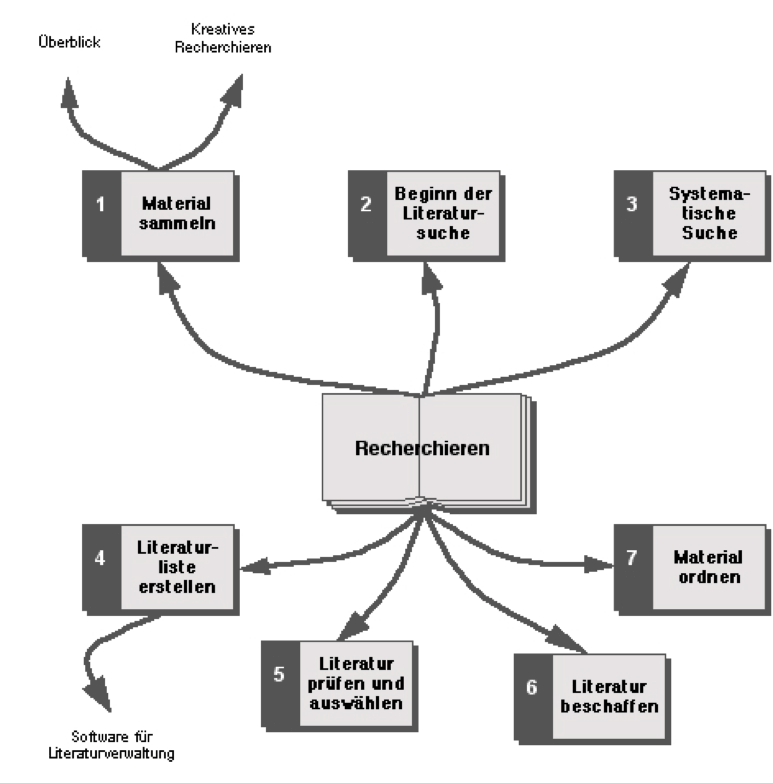
\includegraphics{images/recherchieren-min} 

}

\caption{Recherchieren (Übersicht)}\label{fig:unnamed-chunk-3}
\end{figure}

Bereits beim Konzipieren der Arbeit haben Sie Material gesucht (siehe
Kapitel „Konzipieren einer Arbeit``). Das war aber erst eine vorläufige
Umschau, die Ihnen geholfen hat, ein Thema zu finden und sich einen
Überblick über die zu bearbeitende Literatur dazu zu verschaffen. Jetzt
geht es darum, systematisch die Quellen für die wissenschaftliche Arbeit
zusammenzustellen. Das erste Ergebnis dieser Phase ist eine Leseliste,
die alle Aspekte, die Sie in der Arbeit behandeln wollen, umfasst.
Zusammen mit der Erstellung der Leseliste erheben und entscheiden Sie
auch, wie Sie an die aufgelisteten Quellen herankommen: aus dem Internet
herunterladen, kaufen oder entleihen. Am Ende der Recherche haben Sie
die wesentlichen Materialien für Ihre Arbeit beisammen und verfügbar,
und Sie können mit dem Lesen beginnen. Es kann sich später
herausstellen, dass noch Literatur zur einen oder anderen Frage fehlt
und zusätzlich gesucht, beschafft und gelesen werden muss. Das bringt
aber jedes mal wieder die Gefahr mit sich, dass man sich in erneuter
Literatursuche verzettelt, meint, immer noch mehr lesen zu müssen, und
nie damit fertig wird.

Grundsätzlich gilt: Sie können nie alles zu Ihrem Thema kennen und
lesen! Es gibt heute einfach zu viele Wissenschafterinnen, die alle
ständig schreiben und publizieren, und durch die neuen Möglichkeiten des
Internets, weltweit zu recherchieren, haben Sie potenziell Zugang zu
allen Quellen, Personen und Institutionen, die etwas mit dem Thema zu
tun haben. Es ist daher praktisch unmöglich geworden, sich einen
wirklich vollständigen Überblick über die Literatur zu einem Thema zu
verschaffen. Damit haben heute alle wissenschaftlich Arbeitenden --
sofern sie nicht in einem ganz speziellen, engen und daher (noch)
überschaubaren Gebiet zu Hause sind -- ein neues Problem: Wann ist es
genug? Habe ich die wichtigen Quellen zum Thema gefunden? Was kann ich
weglassen? Es muss daher dem Recherchieren eine vernünftige Grenze
gesetzt werden, die sowohl dem Arbeitsvorhaben in Zeit und Aufwand
angemessen ist als auch auf nachvollziehbaren Auswahlkriterien beruht.

In diesem und dem nächsten Kapitel werden zwei „Hauptstraßen`` des
Recherchierens, jeweils mit mehreren Abzweigungen, beschritten: einmal
die traditionelle Literatursuche in Bibliotheken, in Bibliografien und
im Buchhandel, und einmal die Materialsuche im Internet. Manche
Tätigkeiten, z. B. die Suche im lokalen Bibliothekskatalog, können Sie
sowohl auf die eine als auch auf die andere Art erledigen.

\section{Material sammeln}\label{recherchieren-material-sammeln}

Der erste Teil dieses Abschnitts beschreibt auch die Materialsuche, die
Sie beim Konzipieren einer Arbeit ausführen, um einen Überblick und eine
vorläufige Literaturliste zu erhalten (siehe Kapitel „Konzipieren einer
Arbeit``). Die Phase der Materialsammlung, -sichtung und -auswahl ist im
folgenden Diagramm dargestellt.

\subsection{Überblick}\label{uberblick}

\begin{figure}

{\centering 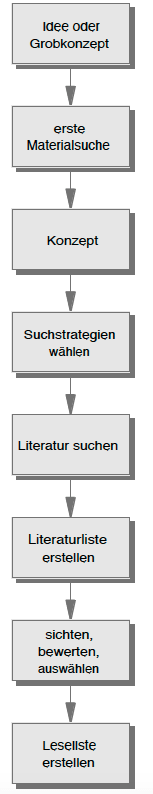
\includegraphics{images/recherchieren-ablauf-min} 

}

\caption{Prozesschritte beim Recherchieren}\label{fig:unnamed-chunk-4}
\end{figure}

Ausgangspunkt ist die Idee oder das Rohkonzept, das aus der Erschließung
des Themas hervorgegangen ist.

Es folgt die dort beschriebene vorläufige Materialsuche. Die
Suchstrategien, Quellen und Techniken, die dafür verwendet werden, sind
im Prinzip dieselben wie die, die Sie für die spätere gründliche
Literatursuche brauchen. Nur erhebt diese erste Suche noch nicht den
Anspruch auf (relative) Vollständigkeit bzw. Repräsentativität. Sie
wollen sich ja zuerst einmal ein Bild vom Stand der Forschung zu Ihrem
geplanten Thema machen und den Aufwand für die Bearbeitung einschätzen.
Ergebnis dieser ersten Phase ist das Konzept.

Bevor Sie mit der eigentlichen Literatursuche beginnen, ist es vor allem
bei größeren wissenschaftlichen Arbeiten von Vorteil, zuerst einen
Suchplan zu machen und die geeigneten Suchstrategien zu wählen: sollten
Sie zuerst in die Bibliothek gehen, in der Buchhandlung stöbern oder im
World Wide Web suchen? Müssen Sie sich mehr auf Bücher oder mehr auf
Zeitschriften konzentrieren? usw.

Gehen Sie bei der Suche nach Ihrem Plan vor: Besonders bei der
Materialsuche im Internet besteht die akute Gefahr, vom Hundertsten ins
Tausendste zu kommen.

Die erste Literaturliste kann in der Form noch ganz beliebig sein:
Zettel, Ausdrucke, Kopien von Literaturverzeichnissen, Lesezeichen im
Internet-Browser. Sie braucht nur so viele Angaben zu enthalten, wie
nötig sind, um dem Hinweis nachgehen zu können, wenn Sie die Quelle
sichten und bewerten wollen.

Im ersten Anlauf sammeln und notieren Sie alles, was Ihnen zum Thema
unterkommt. Durch prüfendes Lesen (siehe Kapitel „Lesen und notieren``)
können Sie relativ rasch feststellen, was Sie davon wirklich brauchen
können und wofür.

Mit diesem Wissen ist es nun möglich, eine Leseliste zu erstellen. Sie
ist die Grundlage für die nächste Phase, in der es darum geht, sich die
Literatur zu beschaffen.

\subsection{Kreatives Recherchieren}\label{kreatives-recherchieren}

Die Literatur für eine Arbeit zusammenzutragen, ist selbst schon ein
guter Teil der kreativen Tätigkeit, die für das wissenschaftliche
Arbeiten erforderlich ist. Deswegen wird diese Fertigkeit ja im Studium
auch schrittweise vermittelt und geübt: Während die Studierenden für
ihre ersten schriftlichen Arbeiten noch ein paar Titel vorgegeben
bekommen, müssen sie später (z. B. in Seminararbeiten) zu einem
vorgegebenen Thema und mit Hilfestellungen bereits selbst zu
recherchieren beginnen. Beim selbstgewählten und -definierten Thema
einer Abschlussarbeit schließlich wird die eigenständige Planung und
Durchführung der Materialsuche auf die Probe gestellt.

Kreativität und Erfindungsreichtum sind hier notwendig, denn die
Fragestellung einer wissenschaftlichen Arbeit entsteht ja gerade aus
einem noch nicht (ganz) gelösten, vernachlässigten oder strittigen
Sachverhalt heraus -- von einer Lücke oder einem Mangel, der einem bei
der ersten überblicksmäßigen Einarbeitung ins Auge gestochen ist. Die
Zielsetzung der Arbeit besteht darin, diese Lücke aufzuzeigen oder (z.
B. in einer Dissertation) sogar einen eigenen Lösungsvorschlag dafür zu
liefern.

Es liegt also beinahe in der Natur der Sache, dass Ihre Fragestellung
von der vorhandenen Literatur gar nicht, nicht ausreichend oder nicht
unter Ihrem Blickwinkel behandelt wird. Selbst wenn Sie in Ihrer Arbeit
keine neuen Argumente oder Theorien entwickeln wollen (oder müssen),
sondern „nur`` einen Überblick über ein Gebiet, eine Schule, eine
Diskussion etc. geben, so werden Sie sich dazu nicht nur auf Literatur
beschränken, die sich „innerhalb`` dieser Schule, dieses Gebiets bewegt,
sondern auch Zusammenfassungen, Klassifikationen, Kritiken von
Außenstehenden berücksichtigen -- schon um selbst Distanz und Überblick
zu gewinnen. Auch für solche Arbeiten gilt es daher, bei der
Materialsuche erfinderisch zu sein.

Das Konzept einer umfangreicheren Arbeit ist meist so komplex, dass es
nicht genügt, Literatur bloß zu genau einem Thema oder einer
Fragestellung zu verwenden. Um Ihren Argumentationsgang zu entwickeln
und zu belegen, werden Sie verschiedenste Materialien brauchen, oft
sogar aus anderen Disziplinen. Diese Notwendigkeit kann schon dort
auftreten, wo Sie ein Anwendungsgebiet, ein Beispiel oder eine
Fallstudie darstellen und beschreiben und dafür den sozio-ökonomischen,
historischen, geografischen etc. Kontext umreißen wollen. (Beispiel: Zu
einem Thema wie „Integration bosnischer Flüchtlingskinder in
Pflichtschulen`` wird der Leser dankbar sein, wenn er erfährt, seit wann
es dieses Problem gibt, wie viele Kinder davon betroffen sind, usw.).
Ein Konzept, anhand dessen man ungefähr sehen kann, aus welchen
Richtungen, Disziplinen usw. und zu welchen Fragen man Literatur
brauchen wird, erweist sich dabei als wichtiger Leitfaden, an dem man
die Materialsuche orientieren kann.

Bevor wir die Strategien der Literatursuche beschreiben, möchten wir
anhand einer Tabelle die Arten von Literatur, die Sie brauchen und mit
der Sie zu tun haben werden, darstellen.

\begin{longtable}[]{@{}lll@{}}
\caption{\textbf{\label{tab:literaturarten} Arten von
Literatur}}\tabularnewline
\toprule
\begin{minipage}[b]{0.31\columnwidth}\raggedright\strut
Sie verwenden\ldots{}\strut
\end{minipage} & \begin{minipage}[b]{0.27\columnwidth}\raggedright\strut
für\ldots{}\strut
\end{minipage} & \begin{minipage}[b]{0.33\columnwidth}\raggedright\strut
Beispiele\strut
\end{minipage}\tabularnewline
\midrule
\endfirsthead
\toprule
\begin{minipage}[b]{0.31\columnwidth}\raggedright\strut
Sie verwenden\ldots{}\strut
\end{minipage} & \begin{minipage}[b]{0.27\columnwidth}\raggedright\strut
für\ldots{}\strut
\end{minipage} & \begin{minipage}[b]{0.33\columnwidth}\raggedright\strut
Beispiele\strut
\end{minipage}\tabularnewline
\midrule
\endhead
\begin{minipage}[t]{0.31\columnwidth}\raggedright\strut
Lexika, Nachschlagewerke\vspace{5mm}\strut
\end{minipage} & \begin{minipage}[t]{0.27\columnwidth}\raggedright\strut
Begriffe, Definitionen, Kurzüberblick über das Thema\vspace{5mm}\strut
\end{minipage} & \begin{minipage}[t]{0.33\columnwidth}\raggedright\strut
Encyclopedia Britannica, Wörterbuch der Psychologie usw.
\vspace{5mm}\strut
\end{minipage}\tabularnewline
\begin{minipage}[t]{0.31\columnwidth}\raggedright\strut
Einführung, Lehrbuch, Sachbuch, Kompendium, Reader\vspace{5mm}\strut
\end{minipage} & \begin{minipage}[t]{0.27\columnwidth}\raggedright\strut
Überblick über das Thema, Auffrischen der Kenntnisse,
„Einlesen``\vspace{5mm}\strut
\end{minipage} & \begin{minipage}[t]{0.33\columnwidth}\raggedright\strut
„Entwicklungspsychologie. Ein Lehrbuch`` \vspace{5mm}\strut
\end{minipage}\tabularnewline
\begin{minipage}[t]{0.31\columnwidth}\raggedright\strut
Primärliteratur \vspace{5mm}\strut
\end{minipage} & \begin{minipage}[t]{0.27\columnwidth}\raggedright\strut
Gegenstand der Arbeit\vspace{5mm}\strut
\end{minipage} & \begin{minipage}[t]{0.33\columnwidth}\raggedright\strut
Jean Piaget, Gesammelte Werke; Zeitungsartikel; Film; Tonträger usw.
\vspace{5mm}\strut
\end{minipage}\tabularnewline
\begin{minipage}[t]{0.31\columnwidth}\raggedright\strut
Sekundärliteratur (wissenschaftliche Werke über die
Primärliteratur)\vspace{5mm}\strut
\end{minipage} & \begin{minipage}[t]{0.27\columnwidth}\raggedright\strut
Analyse, Interpretation, Diskussion der
Primärliteratur\vspace{5mm}\strut
\end{minipage} & \begin{minipage}[t]{0.33\columnwidth}\raggedright\strut
G. Steiner, Piaget und die Folgen \vspace{5mm}\strut
\end{minipage}\tabularnewline
\begin{minipage}[t]{0.31\columnwidth}\raggedright\strut
empirisches Werk\vspace{5mm}\strut
\end{minipage} & \begin{minipage}[t]{0.27\columnwidth}\raggedright\strut
Unterstützung oder Kritik von Argumenten, Datenbasis und
-interpretation\vspace{5mm}\strut
\end{minipage} & \begin{minipage}[t]{0.33\columnwidth}\raggedright\strut
Videofilme von Kleinkindern; wiss. Arbeit, die diese Videos auswertet
\vspace{5mm}\strut
\end{minipage}\tabularnewline
\begin{minipage}[t]{0.31\columnwidth}\raggedright\strut
theoretisches Werk\vspace{5mm}\strut
\end{minipage} & \begin{minipage}[t]{0.27\columnwidth}\raggedright\strut
Rezeption, Kritik, Vergleich, Diskussion,
Theoriebildung\vspace{5mm}\strut
\end{minipage} & \begin{minipage}[t]{0.33\columnwidth}\raggedright\strut
Buch, das empirische Ergebnisse diskutiert und verallgemeinert
\vspace{5mm}\strut
\end{minipage}\tabularnewline
\begin{minipage}[t]{0.31\columnwidth}\raggedright\strut
Praxisbericht (angewandte Theorie \ldots{}) \vspace{5mm}\strut
\end{minipage} & \begin{minipage}[t]{0.27\columnwidth}\raggedright\strut
Beispiel, Fallstudie, Beleg, Interpretation \vspace{5mm}\strut
\end{minipage} & \begin{minipage}[t]{0.33\columnwidth}\raggedright\strut
Tagebuch eines Erziehers \vspace{5mm}\strut
\end{minipage}\tabularnewline
\bottomrule
\end{longtable}

\section{Beginn der Literatursuche}\label{beginn-der-literatursuche}

Wir beschreiben hier auch die Materialsuche, die Sie schon zu Beginn der
Arbeit, zur Themenfindung und Erarbeitung des Konzepts, durchführen. An
diesem Punkt haben Sie möglicherweise noch nichts weiter als ein
Stichwort zum Thema, ein Buch oder einen Artikel, der Sie auf das Thema
gebracht hat, oder ein paar Literaturhinweise aus Lehrveranstaltungen
oder von der Betreuerin. Sie haben also irgendeinen Ausgangspunkt, von
dem aus Sie weitermachen können. Wie Sie sich einen allgemeinen
Überblick zum Thema verschaffen, wurde im Kapitel „Konzipieren einer
Arbeit`` behandelt. Hier geht es nun spezieller um die Literatursuche.

Ausgangspunkt ist ein Schlagwort, ein Fachgebiet, ein einzelnes Werk,
von dem Sie Autor und Titel kennen. Bei der ersten Schlagwortsuche
werden Sie vielleicht schon reichlich „Treffer`` erzielen, vielleicht
sogar zu viele. Trotzdem kann Ihre Suche damit noch nicht beendet sein.
Die meisten Titel, die Sie finden, werden auch unter anderen
Schlagwörtern geführt. Notieren Sie sich diese Schlagwörter und suchen
Sie auch nach ihnen. Auch bei der Suche nach Autor/Titel finden Sie
Schlagwörter, die Sie zur weiteren Suche verwenden können.

\begin{figure}

{\centering 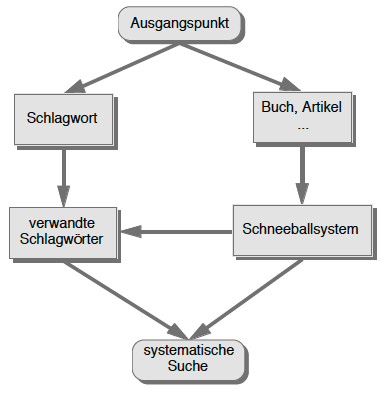
\includegraphics{images/recherchieren-literatursuche-beginn-min} 

}

\caption{Beginn der Literatursuche}\label{fig:unnamed-chunk-5}
\end{figure}

„Schneeballsystem`` bedeutet: Sie haben ein Buch zu Ihrem Thema, in dem
wieder andere Bücher behandelt und mit bibliografischen Angaben zitiert
werden. Sie finden diese angegebenen Bücher und behandeln Sie in Ihrer
Arbeit. Diese Bücher haben ebenfalls Literaturangaben, und so finden Sie
noch mehr Literatur, usw. Abgesehen davon, dass man manchmal gar nicht
anders kann, als jeden Hinweis aufzugreifen, hat das System den Vorteil,
dass man oft sehr schnell auf die „Schlüsselwerke`` oder „Klassiker`` zu
einem Thema stößt: Ein Werk, das von vielen oder allen
Wissenschafterinnen, die zu diesem Thema arbeiten, zitiert wird, ist
wahrscheinlich eines, das Sie auch nicht übergehen dürfen. Die Gefahr
dabei ist, dass Sie in eine „Zitierbruderschaft`` geraten, also in eine
Gruppe, Richtung oder Schule von Wissenschaftern, die sich hauptsächlich
gegenseitig lesen und/oder zitieren. Die Erweiterung und
Systematisierung der Suche bleibt einem also trotzdem nicht erspart.

Viele Titel, die Sie bei Ihrer ersten Recherche in Bibliothekskatalogen
finden, sind unter mehreren Schlagwörtern katalogisiert. Noch gibt es
keine für den deutschen Sprachraum genormte Schlagwortliste, sodass die
Einträge sogar von einer Universitätsbibliothek zur anderen variieren
können. Vor allem wenn die Suche nach einem Schlagwort, das Ihnen
treffend erscheint, unbefriedigend verläuft, müssen Sie diese verwandten
Begriffe für die spätere systematische Suche notieren. Überlegen Sie
sich auch mögliche Synonyme, Überbegriffe, ähnliche (oft auch ältere
oder veraltete) Begriffe für das von Ihnen Gesuchte.

\section{Systematische Suche}\label{systematische-suche}

Außer bei frühen „Übungsarbeiten`` im Studium (Proseminare u. dgl.), wo
Sie erst einmal zeigen sollen, dass Sie überhaupt imstande sind,
Bibliotheken und Kataloge zu benutzen und Literatur zu finden, ist
dieser erste Durchgang bei der Literatursuche nicht ausreichend. Sie
müssen einen zweiten Durchgang, die systematische Suche, anschließen.

\begin{figure}

{\centering 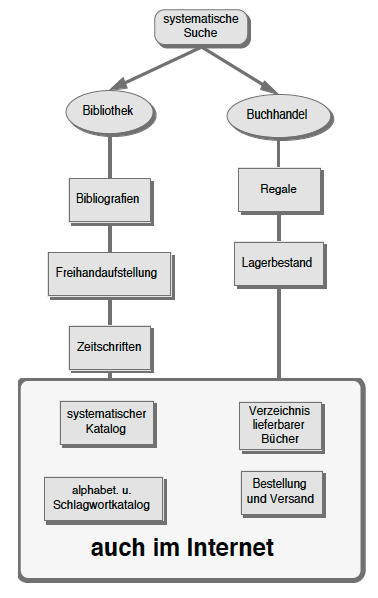
\includegraphics{images/recherchieren-literatursuche-systematisch-min} 

}

\caption{Sytematische Literatursuche}\label{fig:unnamed-chunk-6}
\end{figure}

Grundsätzlich gibt es dazu zwei Möglichkeiten: die Online-Suche im
Internet (siehe Kapitel „Recherchieren im Internet``) und die
„Turnschuh-Methode``, d. h. in Bibliotheken, Buchhandlungen usw. gehen
und vor Ort suchen. Selbst in Zeiten, wo man schon beinahe alles über
das Internet erledigen kann, sollte man auf die Suche vor Ort nicht ganz
verzichten:

In einer Bibliothek mit Freihandaufstellung (Präsenzbibliothek) oder in
den Regalen einer (großen) Buchhandlung hat man den Vorteil, dass man
die zu einem Fachgebiet vorhandenen Werke gleich beisammen hat und sich
sofort selbst ein Bild davon machen kann. Oft sind nämlich selbst
inhaltlich eng verwandte Bücher unter verschiedenen Schlagwörtern
erfasst, und man würde bei einer Suche im Katalog niemals darauf stoßen.
Solche „zufälligen`` Fundstücke ergänzen und erweitern die systematische
Suche -- auch weil sie einen auf weitere Titel und Schlagwörter bringen
können.

Früher führten Universitätsbibliotheken drei Kataloge: den
alphabetischen (geordnet nach Autor bzw. Ordnungswort), den
systematischen (nach Aufstellung, Nummerierung etc. der Bibliothek) und
den Schlagwortkatalog (oder Deskriptoren = Begriffe, die den Inhalt des
Werks beschreiben). Heute genügt eine einzige Datenbank, die nach
mehreren Feldern durchsucht werden kann, u. a. auch nach Stichwörtern (=
Wörter, die im Titel oder Text vorkommen). Das folgende Beispiel einer
elektronischen Karte aus einem OPAC (Open Public Access Catalogue) zeigt
die Hinweise für die weitere Suche bzw. Beschaffung eines Werks.

\begin{figure}

{\centering 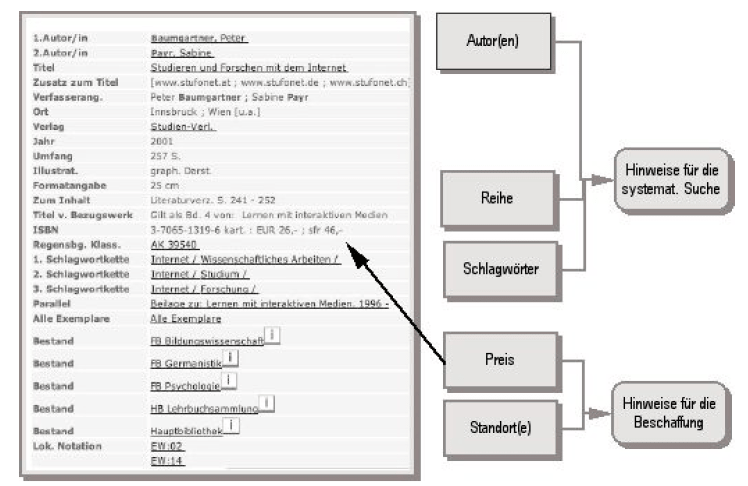
\includegraphics{images/recherchieren-OPAC-Karteikarte-min} 

}

\caption{Elektronische Karteikarte aus einem OPAC}\label{fig:unnamed-chunk-7}
\end{figure}

Das Verzeichnis lieferbarer Bücher (VLB) ist der „Katalog`` des
Buchhandels, der regelmäßig aktualisiert wird. Man kann in ihm nach
Autoren, Titeln und Schlagwörtern suchen. In Buchhandlungen kann man
eine solche Recherche durchführen und sich das Ergebnis ausdrucken
lassen. Das VLB ist ein Service für den Buchhandel und im Internet
kostenpflichtig. Allerdings gibt es Online-Buchhandlungen, deren
Datenbestand auf dem VLB beruht (ob aktuell oder tatsächlich, ist zum
Teil allerdings nicht ersichtlich). Das VLB wird seinem Namen nicht
hundertprozentig gerecht: weder sind alle lieferbaren Titel erfasst (das
hängt vom Verlag ab), noch sind immer alle Titel wirklich lieferbar.

Die Elektronische Zeitschriftenbibliothek (EZB) ist ein Service zur
effektiven Nutzung wissenschaftlicher Volltextzeitschriften im Internet.
Dieser Dienst wird inzwischen in 343 Bibliotheken bzw.
Forschungseinrichtungen im deutschsprachigen Raum angeboten. Die Titel
werden kooperativ gesammelt und die Daten gemeinsam in einer zentralen
Datenbank gepflegt. Jede beteiligte Institution kann ihre lizenzierten
Zeitschriften eigenständig verwalten und eigene Benutzerhinweise
integrieren. Abonnierte Volltextzeitschriften können zusammen mit frei
zugänglichen E-Journals in einer einheitlichen Oberfläche angeboten
werden. Eine „Ampel`` zeigt die Zugriffsrechte auf eine Zeitschrift an
der jeweiligen Bibliothek an. Allerdings: weder die EZB noch die ZDB
(Zeitschriftendatenbank, weist Bestand in Deutschland nach) ermöglichen
es, nach Artikeln in Zeitschriften zu suchen.

Bibliografien sind gedruckte oder elektronische Literaturverzeichnisse,
die ebenfalls regelmäßig aktualisiert werden. Hier werden auch
unselbständig erschienene Werke, v. a. Zeitschriftenartikel, erfasst.
Der Nachteil ist, dass Bibliografien nie ganz aktuell sind -- es vergeht
eben eine geraume Zeit zwischen dem Erscheinen eines Artikels und seiner
Erfassung bzw. Veröffentlichung in einer Bibliografie.

Jede Methode hat also ihre Stärken und Schwächen. Sie müssen miteinander
kombiniert werden, wenn man wirklich systematisch vorgehen will. Hier
sind die Vor- und Nachteile im Überblick:

\begin{longtable}[]{@{}lllll@{}}
\caption{\textbf{\label{tab:literatur-suchen} Ergebnisse der
Literatursuche}}\tabularnewline
\toprule
\begin{minipage}[b]{0.21\columnwidth}\raggedright\strut
Ergebnisse, bezogen auf\ldots{}\strut
\end{minipage} & \begin{minipage}[b]{0.18\columnwidth}\raggedright\strut
Bibliotheks-kataloge\strut
\end{minipage} & \begin{minipage}[b]{0.16\columnwidth}\raggedright\strut
Fachbiblio-grafien\strut
\end{minipage} & \begin{minipage}[b]{0.14\columnwidth}\raggedright\strut
VLB\strut
\end{minipage} & \begin{minipage}[b]{0.18\columnwidth}\raggedright\strut
UB-Kataloge online\strut
\end{minipage}\tabularnewline
\midrule
\endfirsthead
\toprule
\begin{minipage}[b]{0.21\columnwidth}\raggedright\strut
Ergebnisse, bezogen auf\ldots{}\strut
\end{minipage} & \begin{minipage}[b]{0.18\columnwidth}\raggedright\strut
Bibliotheks-kataloge\strut
\end{minipage} & \begin{minipage}[b]{0.16\columnwidth}\raggedright\strut
Fachbiblio-grafien\strut
\end{minipage} & \begin{minipage}[b]{0.14\columnwidth}\raggedright\strut
VLB\strut
\end{minipage} & \begin{minipage}[b]{0.18\columnwidth}\raggedright\strut
UB-Kataloge online\strut
\end{minipage}\tabularnewline
\midrule
\endhead
\begin{minipage}[t]{0.21\columnwidth}\raggedright\strut
Inhalt\vspace{5mm}\strut
\end{minipage} & \begin{minipage}[t]{0.18\columnwidth}\raggedright\strut
Bestand d. Bibliothek\vspace{5mm}\strut
\end{minipage} & \begin{minipage}[t]{0.16\columnwidth}\raggedright\strut
alle Titel\vspace{5mm}\strut
\end{minipage} & \begin{minipage}[t]{0.14\columnwidth}\raggedright\strut
alle lieferbaren Titel\vspace{5mm}\strut
\end{minipage} & \begin{minipage}[t]{0.18\columnwidth}\raggedright\strut
erfasster Bestand einer od. mehrerer Bibliotheken \vspace{5mm}\strut
\end{minipage}\tabularnewline
\begin{minipage}[t]{0.21\columnwidth}\raggedright\strut
Vollständigkeit \vspace{5mm}\strut
\end{minipage} & \begin{minipage}[t]{0.18\columnwidth}\raggedright\strut
nein -- nur Bestand \vspace{5mm}\strut
\end{minipage} & \begin{minipage}[t]{0.16\columnwidth}\raggedright\strut
ja, bis Stichtag\vspace{5mm}\strut
\end{minipage} & \begin{minipage}[t]{0.14\columnwidth}\raggedright\strut
nein (vergriffene Titel!) \vspace{5mm}\strut
\end{minipage} & \begin{minipage}[t]{0.18\columnwidth}\raggedright\strut
nein -- nur erfasste Bestände \vspace{5mm}\strut
\end{minipage}\tabularnewline
\begin{minipage}[t]{0.21\columnwidth}\raggedright\strut
Artikel (unselbständige Werke) \vspace{5mm}\strut
\end{minipage} & \begin{minipage}[t]{0.18\columnwidth}\raggedright\strut
nein \vspace{5mm}\strut
\end{minipage} & \begin{minipage}[t]{0.16\columnwidth}\raggedright\strut
ja \vspace{5mm}\strut
\end{minipage} & \begin{minipage}[t]{0.14\columnwidth}\raggedright\strut
nein \vspace{5mm}\strut
\end{minipage} & \begin{minipage}[t]{0.18\columnwidth}\raggedright\strut
nein \vspace{5mm}\strut
\end{minipage}\tabularnewline
\begin{minipage}[t]{0.21\columnwidth}\raggedright\strut
Vorteil \vspace{5mm}\strut
\end{minipage} & \begin{minipage}[t]{0.18\columnwidth}\raggedright\strut
vor Ort verfügbar, entlehnbar \vspace{5mm}\strut
\end{minipage} & \begin{minipage}[t]{0.16\columnwidth}\raggedright\strut
Vollständigkeit \vspace{5mm}\strut
\end{minipage} & \begin{minipage}[t]{0.14\columnwidth}\raggedright\strut
sofort bestellbar \vspace{5mm}\strut
\end{minipage} & \begin{minipage}[t]{0.18\columnwidth}\raggedright\strut
vor Ort od. per Fernleihe entlehnbar \vspace{5mm}\strut
\end{minipage}\tabularnewline
\begin{minipage}[t]{0.21\columnwidth}\raggedright\strut
Problem \vspace{5mm}\strut
\end{minipage} & \begin{minipage}[t]{0.18\columnwidth}\raggedright\strut
nur selbständige Werke \vspace{5mm}\strut
\end{minipage} & \begin{minipage}[t]{0.16\columnwidth}\raggedright\strut
Titel z. T. nicht beschaffbar; nicht (ganz) aktuell \vspace{5mm}\strut
\end{minipage} & \begin{minipage}[t]{0.14\columnwidth}\raggedright\strut
nur selbst. Werke, Aufnahme ist Sache des Verlags \vspace{5mm}\strut
\end{minipage} & \begin{minipage}[t]{0.18\columnwidth}\raggedright\strut
nur selbst. Werke, ab wann erfasst? vollständige Ausgabe der Treffer?
\vspace{5mm}\strut
\end{minipage}\tabularnewline
\bottomrule
\end{longtable}

Um eine halbwegs vollständige Literaturliste zu erstellen, kommen Sie
also um einen Besuch der Universitätsbibliothek nicht herum. Nur hier
haben Sie Zugang zu Bibliografien und Verzeichnissen unselbständig
erschienener Schriften (damit sind v. a. Zeitschriftenartikel gemeint).
Trotz aller Hilfsmittel sollten Sie sich aber nicht das Ziel stecken,
eine wirklich vollständige Literaturliste zu erstellen -- außer, das ist
selbst schon das Thema Ihrer Arbeit. In diesem Fall tun Sie aber nichts
außer Literatur suchen und erfassen. Für jede andere Arbeit, wo Sie die
Literatur auch noch auswählen, lesen, rezipieren und diskutieren müssen,
wäre das zu viel verlangt. Es gibt inzwischen einfach zu viele
Wissenschafterinnen und Studierende, die Arbeiten schreiben müssen, als
dass vernünftigerweise gefordert werden könnte, alles auch nur zu
finden.

Meistens wird man deshalb einen mehr oder weniger willkürlichen
Schlussstrich unter die Materialsuche ziehen müssen. Zum einen sollte
man sich schon vorher einen Termin setzen und sich auch daran halten,
auch wenn man mit den Suchergebnissen noch nicht ganz zufrieden ist und
die Literaturliste noch einige Lücken aufweist. Bei der Ausarbeitung der
Argumentation wird meistens sowieso noch die eine oder andere Frage
auftauchen, zu der speziell und gezielt noch Literatur gefunden werden
muss. Zum anderen kann man die Literatursuche als abgeschlossen
betrachten, wenn zu jedem im Konzept aufgeführten Teil oder Argument
Material gefunden wurde. Schon deshalb ist es sinnvoll, bei der
Literatursuche immer das Exposé der Arbeit dabeizuhaben und auch hin und
wieder hineinzuschauen. So kann man gleich die gefundenen Titel
vorläufig dem Konzept zuordnen und sich auch orientieren, in welche
Richtung Material gesucht werden muss.

\section{Literaturliste erstellen}\label{literaturliste-erstellen}

Selbst der größte Chaot wird manchmal gezwungen, so etwas wie Ordnung zu
schaffen. Die Literatursuche für eine wissenschaftliche Arbeit ist so
ein Fall: ein wenig Ordnung erspart viel zusätzliche und doppelte
Arbeit, für die dann später sowieso nicht genug Zeit bleibt.

Gleich wo und wie Sie Literatur für Ihre Arbeit suchen: halten Sie die
Ergebnisse systematisch fest. Erfassen Sie auch Werke, die Ihnen im
Augenblick als nur marginal interessant oder brauchbar erscheinen: es
kann ja durchaus passieren, dass Sie das Konzept Ihrer Arbeit noch
ändern und dann gerade diesen Titel brauchen würden. Die Literaturliste
sollte möglichst vollständig sein, auch wenn Sie dann nur einen Teil
davon tatsächlich zum Bearbeiten auswählen.

Die „klassische`` Methode für die Zusammenstellung ist der Zettel- oder
Karteikasten. Sie legen für jeden Titel eine eigene Karte (oder einen
Zettel entsprechender Größe) an. Wenn Sie „vor Ort`` in Bibliotheken und
Buchhandlungen suchen, können Sie Ihre Funde direkt auf Karteikarten
notieren. Ausdrucke aus Datenbanken oder dem Internet müssen entweder
nochmals geschrieben oder ausgeschnitten und aufgeklebt werden. Jede
Karte sollte alle bibliografischen Angaben haben, die für ein
Literaturverzeichnis möglicherweise gebraucht werden (siehe Kapitel
„Zitieren``):

\begin{itemize}
\tightlist
\item
  Name des Autors bzw. der Autoren: alle Namen mit Vor- und Zunamen
  (soweit eruierbar),
\item
  Titel und Untertitel
\item
  Erscheinungsjahr, Auflage, Band, sonstige Angaben (wie: Abdruck,
  Überarbeitung, Übersetzer, \ldots{})
\item
  Verlag, Erscheinungsort
\item
  bei Zeitschriftenartikeln: Name der Zeitschrift, Jahrgang, Heft,
  Seiten (von - bis)
\item
  bei Beiträgen in Sammelbänden: Herausgeber, bibliograf. Angaben des
  Sammelbandes (s. oben), Seiten (von - bis)
\item
  URL und Datum des Fundes im Internet (s. Kapitel XXX)
\end{itemize}

Zusätzlich können (und sollten) Sie auf der Karteikarte Dinge vermerken,
die für die Auswahl und Beschaffung des Werks von Bedeutung sind: der
Standort, die Signatur bzw. Systematik, den Preis, ob es gerade
entliehen ist, usw.

Die Karteikarten werden alphabetisch nach den AutorInnen geordnet. Es
wäre zu aufwändig, ein eigenes Schlagwortsystem (z. B. nach dem Exposé)
einzuführen und durchzuhalten -- das Konzept der Arbeit kann sich ja
noch ändern. Andersherum ist es aber durchaus sinnvoll, das Exposé jetzt
zu überarbeiten und zu jedem geplanten Abschnitt und Argument auch
(vorläufig und versuchsweise) die dazu zu bearbeitende Literatur
hinzuzufügen (Autor, Titel oder Kurzbeleg genügen völlig, solange Sie
das gemeinte Werk dadurch identifizieren können).

\subsection{Software für
Literaturverwaltung}\label{software-fur-literaturverwaltung}

Ein „elektronischer Zettelkasten`` in Form einer Datenbank oder
speziellen Literaturverwaltungssoftware erspart einem zwar nicht das
Erfassen jeden Titels, kann aber bei weiteren Arbeitsschritten sehr
nützlich sein:

\begin{itemize}
\tightlist
\item
  Datenbanken lassen sich nach verschiedenen Kriterien durchsuchen und
  sortieren. Sie finden also später auch ein Werk, von dem Sie nur mehr
  den Titel wissen, aber partout nicht mehr den Autor.
\item
  Sie können verschiedene Listen und Ausdrucke erstellen
\item
  Oft können auch Notizen, Exzerpte, Zusammenfassungen usw. zusammen mit
  den bibliografischen Angaben gespeichert werden und gehen nicht
  verloren.
\item
  Mit geeigneter Software (hier kommt es auf das „Zusammenpassen`` der
  Textverarbeitung mit der Literaturverwaltung an) ersparen Sie sich
  sogar das mühsame Schreiben eines Literaturverzeichnisses. Diese
  Programme durchsuchen Texte nach Kurzbelegen (siehe Kapitel
  „Zitieren``) in einer bestimmten Form und erstellen dazu die
  Literaturangabe in einem vorher gewählten Format.
\item
  Literaturverwaltungsprogramme können auch meistens Angaben direkt aus
  bestimmten Datenbankformaten (z. B. OPACs) übernehmen.
\end{itemize}

Bei der Suche „vor Ort``, wo Sie Literaturangaben handschriftlich
aufzeichnen, bleibt Ihnen bei der Verwendung von Software das
nachträgliche Erfassen nicht erspart. Diese zusätzliche Arbeit zahlt
sich aber bereits für eine einzelne größere Arbeit später aus -- und
erst recht, wenn Sie in Zukunft weiter in diesem Gebiet arbeiten werden
oder z. B. Ihre Arbeit auch in Buchform oder als Artikel publizieren
wollen.

\begin{longtable}[]{@{}l@{}}
\caption{\textbf{\label{tab:literatur-erfassen} Literatur suchen und
erfassen}}\tabularnewline
\toprule
\begin{minipage}[t]{0.97\columnwidth}\raggedright\strut
\begin{itemize}
\tightlist
\item
  Habe ich bei der Suche alle Arten von Literatur berücksichtigt?
  \vspace{-6mm}
\end{itemize}\strut
\end{minipage}\tabularnewline
\begin{minipage}[t]{0.97\columnwidth}\raggedright\strut
\begin{itemize}
\tightlist
\item
  Habe ich alle nötigen Kataloge, Verzeichnisse und sonstigen Suchhilfen
  ausgeschöpft? \vspace{-6mm}
\end{itemize}\strut
\end{minipage}\tabularnewline
\begin{minipage}[t]{0.97\columnwidth}\raggedright\strut
\begin{itemize}
\tightlist
\item
  Habe ich alle Themen und Fragestellungen des Exposés (vorläufig)
  abgedeckt? \vspace{-6mm}
\end{itemize}\strut
\end{minipage}\tabularnewline
\begin{minipage}[t]{0.97\columnwidth}\raggedright\strut
\begin{itemize}
\tightlist
\item
  Habe ich alle gefundenen Quellen mit vollständigen bibliografischen
  Angaben und sonstigen Hinweisen erfasst? \vspace{-6mm}
\end{itemize}\strut
\end{minipage}\tabularnewline
\begin{minipage}[t]{0.97\columnwidth}\raggedright\strut
\begin{itemize}
\tightlist
\item
  Ist meine Literaturliste im Rahmen des Möglichen und (für meine
  Arbeit) Erforderlichen vollständig, ausgewogen und aktuell?
  \vspace{-6mm}
\end{itemize}\strut
\end{minipage}\tabularnewline
\begin{minipage}[t]{0.97\columnwidth}\raggedright\strut
\begin{itemize}
\tightlist
\item
  Kann ich die Suche beenden?
\end{itemize}\strut
\end{minipage}\tabularnewline
\bottomrule
\end{longtable}

\section{Literatur prüfen und auswählen -- Leseliste
erstellen}\label{literatur-prufen-und-auswahlen-leseliste-erstellen}

Der nächste Schritt führt nun von der wahrscheinlich sehr umfangreichen
Literaturliste zur eigentlichen Leseliste: Das sind jene Werke, von
denen Sie zum jetzigen Stand der Arbeit und des Konzepts wissen, dass
Sie sie lesen und bearbeiten müssen und dass sie in der Arbeit
Verwendung finden werden. Dazu brauchen Sie jetzt nicht nur Titel und
Autor, sondern müssen schon ein wenig hineinsehen -- das heißt aber noch
nicht, dass Sie alles lesen müssen. Dafür eignen sich die Techniken des
„prüfenden Lesens`` (siehe Kapitel „Lesen und notieren``)

In einer Buchhandlung oder Präsenzbibliothek wird es nicht weiter
schwerfallen, in Bücher hineinzuschauen und in ihnen zu blättern. Etwas
umständlicher ist es bei Bibliotheken mit Magazinen: Sie müssen eine
ganze Reihe Bücher entlehnen, nur um dann vielleicht den Großteil davon
bald wieder zurückzugeben. Um nicht allzuviel Zeit damit zu verlieren,

\begin{itemize}
\tightlist
\item
  gehen Sie mit Ihrer Literaturliste (bzw. jenem Teil davon, der vor Ort
  in der Bibliothek verfügbar ist) hin und entleihen Sie so viele Titel,
  wie Sie bewältigen können.
\item
  tragen Sie diese Bücher nicht nach Hause, sondern prüfen Sie sie
  gleich im Lesesaal.
\end{itemize}

\begin{figure}

{\centering 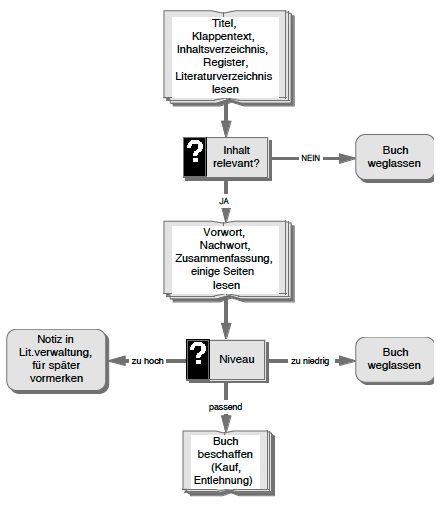
\includegraphics{images/recherchieren-literatur-auswaehlen-min} 

}

\caption{Litertur prüfen und auswählen}\label{fig:unnamed-chunk-8}
\end{figure}

Machen Sie sich bei jenen Werken, die Sie wieder zurückgeben, eine
Notiz, warum Sie dieses Buch ausschließen, am besten zusammen mit einer
kurzen Inhaltsangabe: möglicherweise wird dieses Buch doch später noch
relevant. Manche Titel scheinen das Thema genau zu treffen und sind
trotzdem nicht relevant, sodass man in Gefahr ist, immer wieder, z. B.
bei einer späteren zusätzlichen Literatursuche, auf sie
„hineinzufallen``. Das lässt sich mit dieser Notiz vermeiden, die in der
Literaturkartei bzw. der Datenbank beim Titel erfasst wird.

Wenn ein Buch nur über Fernleihe zugänglich ist bzw. im Buchhandel nicht
lagernd ist, wird diese Relevanzprüfung nicht möglich sein. Kaufen wird
man so eine „Katze im Sack`` sicher erst, wenn man genügend Hinweise
(aus der Literatur, von Betreuern etc.) hat, dass dieses Buch dafür in
Frage kommt (siehe „Literatur beschaffen``). Beim Buchversand im
Internet wird man zwar manchmal eine kurze Inhaltsangabe oder einen
Auszug aus dem Inhaltsverzeichnis finden, aber das ist nicht mehr als
der Text, den ein Verlag in seinen Werbeprospekt drucken würde -- also
nicht unbedingt ein verlässlicher Hinweis auf Brauchbarkeit und
Qualität.

Soweit Sie aber die Titel Ihrer Literaturliste auf Relevanz prüfen
können, lässt sich daraus eine Leseliste zusammenstellen. Wieder ist es
vorteilhaft, sich dabei am Konzept zu orientieren und zu prüfen, ob alle
geplanten Teile ausreichend abgedeckt sind. Diese Prüfung der Literatur
ergibt auch Hinweise darauf, in welcher Reihenfolge Sie die ausgewählten
Titel bearbeiten sollten: wenn ein Autor z. B. ausführlich ein Werk
rezipiert und kritisiert, das ebenfalls auf Ihrer Leseliste steht, liegt
es nahe, zuerst das „Ausgangswerk`` und dann das darauf aufbauende Buch
zu lesen.

Das Endergebnis der Literaturauswahl ist somit eine Leseliste, die
sowohl nach Prioritäten als auch -- ansatzweise -- chronologisch
geordnet ist. Wenn Sie wissen, wie schnell oder langsam Sie lesen,
können Sie die Leseliste anhand Ihres Zeitplans einteilen in jene Titel,
die Sie -- vorsichtig geschätzt -- in der verfügbaren Zeit bearbeiten
können. Es muss dabei aber ein Spielraum bleiben, denn es können während
der Arbeit noch Titel dazukommen, die Sie ebenfalls berücksichtigen
müssen. Es ist also besser, die Lesezeit nur zum Teil zu verplanen und
sich einen fixen Termin für Rückblick, weitere Literaturauswahl bzw.
-suche zu setzen.

\section{Litertur beschaffen}\label{litertur-beschaffen}

\subsection{Bücher beschaffen}\label{bucher-beschaffen}

Welche Bücher soll man sich selbst kaufen, welche soll man entlehnen? Es
gibt Wissenschafterinnen, die mit entlehnten Büchern überhaupt nicht
arbeiten wollen -- sie müssen eben viel Geld investieren, um sich alles
zu kaufen, was sie brauchen. Bei „professionell`` wissenschaftlich
Arbeitenden, die oft lange Zeit an ein und demselben Thema arbeiten, ist
der Kauf sicher öfter eine sinnvolle Lösung als bei Studierenden, die
nach ihrem Studienabschluss mit einem Thema kaum mehr zu tun haben
werden. Auch sie stehen aber vor der Entscheidung, die von einigen
Faktoren, nicht nur vom persönlichen Arbeitsstil, abhängt:

Es gibt noch eine weitere Möglichkeit: die Betreuerin dafür zu
interessieren, das Buch über das Institut oder die
Universitätsbibliothek zu bestellen. Allerdings muss man hier die oft
monatelangen Fristen zwischen der Bestellung eines Buchs und seinem
Auftauchen in einer Universitätsbibliothek berücksichtigen -- sodass das
Buch möglicherweise für die geplante Arbeit zu spät kommt.

\begin{figure}

{\centering 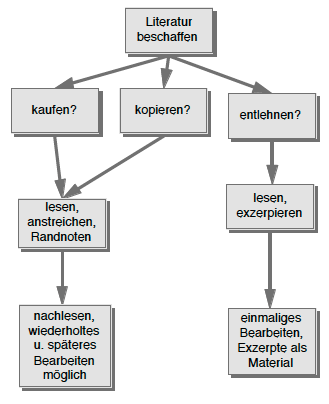
\includegraphics{images/recherchieren-literatur-beschaffen-min} 

}

\caption{Optionen der Literaturbeschaffung}\label{fig:unnamed-chunk-9}
\end{figure}

Weitere Kriterien sind: für KAUFEN: Primärtext, Standardwerk, mehrmalige
Verwendung, Preis (Taschenbuch) für ENTLEIHEN: vergriffen, Querlesen,
zusätzliche Literatur, zu teuer für KOPIEREN: Zeitschriftenartikel,
einzelne Beiträge in Sammelbänden, Lexikonartikel. Graue Papiere,
Forschungsberichte etc. können oft kostenlos oder gegen einen geringen
Kostenersatz bei den AutorInnen angefordert werden. Oft sind sie auch
schon aus dem Internet abrufbar (siehe Kapitel XXX „Recherchieren im
Internet``).

Ein besonderes Problem stellen manchmal Titel dar, die weder in den
Bibliotheken vorhanden sind noch über den Buchhandel einfach bestellt
werden können. Das sind vor allem fremdsprachige wissenschaftliche Werke
in Fachgebieten, wo diese Fremdsprache nicht zum Alltag gehört.
Bücherbestellungen im Ausland sind kompliziert und dauern oft lange. Der
elektronische Buchversand funktioniert allerdings zusehends
international. Englischsprachige Literatur etwa ist problemlos zu
beschaffen, allerdings sollten sie gerade bei beschränktem Zeitbudget
auf die angegebenen voraussichtlichen Lieferfristen achten.

\subsection{Unselbständige Werke
beschaffen}\label{unselbstandige-werke-beschaffen}

Im Vergleich zur relativ einfachen Beschaffung eines Buches kann die
Beschaffung eines bestimmten Zeitschriftenartikels durchaus zu einer
Schnitzeljagd ausarten. Hinweise auf Zeitschriftenartikel, die für Ihre
Arbeit wichtig sein könnten, erhalten Sie meist aus den Referenzen in
anderen Artikeln oder Büchern. Elektronische Zeitschriftenkataloge geben
Ihnen Aufschluss darüber, wo und ob Sie Zugriff auf die Texte haben.
Führt Ihre Bibliothek die Zeitschrift elektronisch oder in Papierform,
so ist das Problem noch einfach zu lösen. Wenn das nicht der Fall ist,
müssen Sie weitersuchen.

\begin{figure}

{\centering 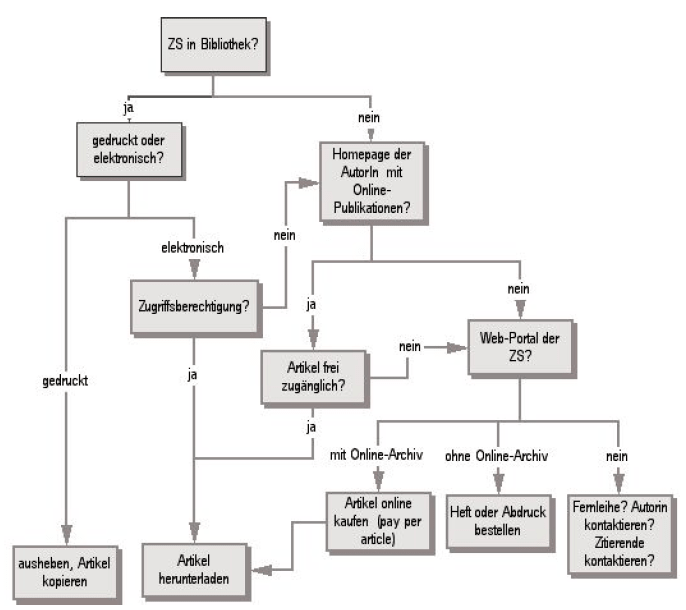
\includegraphics{images/recherchieren-zeitschriften-beschaffen-min} 

}

\caption{Zeitschriftenartikel beschaffen}\label{fig:unnamed-chunk-10}
\end{figure}

Abb.: Zeitschriftenartikel beschaffen

Die Homepage des oder eines Autors ist ein guter Ausgangspunkt dafür:
wenn Sie Glück haben, finden Sie dort im Publikationsverzeichnis den
Artikel zum Herunterladen, und womöglich noch weitere für Sie relevante
vom selben Autor. Manchmal werden Sie nicht genau den gesuchten
Zeitschriftenartikel zum Herunterladen finden (das hat mit der Politik
der Zeitschriftenverlage zu tun, die ihre -- meist sehr teuren --
Zeitschriftenabonnements verkaufen wollen und das Copyright an den
Artikeln haben), sondern vielleicht einen thematisch eng verwandten oder
eine Vorversion. Für kleinere Arbeiten, bei denen Ihr Zeitbudget für die
Recherche und Beschaffung beschränkt ist, können Sie sich meist auch
damit begnügen.

Auch bei anderen unselbständig erschienen Werken, wie etwa Kapiteln in
Sammelbänden oder Konferenzbeiträgen, können Sie bei den Autoren fündig
werden. Wenn nicht, müssen Sie das entsprechende Buch bzw. die
elektronische Gesamtpublikation suchen.

Die Zeitschriftenverlage selbst bieten entweder einzelne Artikel oder
Hefte zum Kauf an, entweder zum Herunterladen mit elektronischem
Zahlungsverkehr oder über den herkömmlichen Bestellweg.

Wenn Sie auch damit keinen Erfolg haben, den besagten Artikel aber
unbedingt benötigen, können Sie die Herausgeber der Zeitschrift oder die
Autoren persönlich kontaktieren.

\begin{longtable}[]{@{}l@{}}
\caption{\textbf{\label{tab:literatur-beschaffen} Literatur auswählen und
beschaffen}}\tabularnewline
\toprule
\begin{minipage}[t]{0.97\columnwidth}\raggedright\strut
\begin{itemize}
\tightlist
\item
  Habe ich die Titel der Literaturliste so weit wie möglich auf ihre
  Relevanz geprüft? \vspace{-6mm}
\end{itemize}\strut
\end{minipage}\tabularnewline
\begin{minipage}[t]{0.97\columnwidth}\raggedright\strut
\begin{itemize}
\tightlist
\item
  Entspricht die Leseliste meinem Zeitplan und den Erfordernissen des
  Themas? \vspace{-6mm}
\end{itemize}\strut
\end{minipage}\tabularnewline
\begin{minipage}[t]{0.97\columnwidth}\raggedright\strut
\begin{itemize}
\tightlist
\item
  Habe ich entschieden, wie ich mir die Titel der obersten
  Prioritätsstufe beschaffe (kaufen, entleihen, kopieren,
  anfordern)?\vspace{-6mm}
\end{itemize}\strut
\end{minipage}\tabularnewline
\begin{minipage}[t]{0.97\columnwidth}\raggedright\strut
\begin{itemize}
\tightlist
\item
  Habe ich Fernleihe und Buchbestellungen im Ausland so früh wie möglich
  in die Wege geleitet (Wartezeiten)?\vspace{-6mm}
\end{itemize}\strut
\end{minipage}\tabularnewline
\begin{minipage}[t]{0.97\columnwidth}\raggedright\strut
\begin{itemize}
\tightlist
\item
  Steht die (vorläufige) Reihenfolge der Bearbeitung der Leseliste fest?
  \vspace{-6mm}
\end{itemize}\strut
\end{minipage}\tabularnewline
\begin{minipage}[t]{0.97\columnwidth}\raggedright\strut
\begin{itemize}
\tightlist
\item
  Habe ich mir einen Termin für das Ende der ersten Lesephase gesetzt?
\end{itemize}\strut
\end{minipage}\tabularnewline
\bottomrule
\end{longtable}

\section{Material ordnen}\label{material-ordnen}

Leben Sie nun zwischen Stößen von Büchern, Notizzetteln, kopierten
Artikeln und Buchauszügen, ausgedruckten Webseiten usw.? Müssen Sie
jedesmal, wenn Sie einen Artikel suchen, mehrere Stapel umschichten und
durchsuchen? Dann wird es Zeit, die Materialien in eine Ordnung zu
bringen, die Ihnen die Arbeit erleichtert. Besonders die „kleinen``
Papiere -- Artikel, eigene Notizen und Ausdrucke, Kopien usw. -- machen
dabei Probleme. Hier sind einige Möglichkeiten, wie Sie damit umgehen
können:

Beim Ablegen von Artikeln in Ordnern ist es ratsam, ein
Inhaltsverzeichnis anzulegen und obenauf einzulegen. Zusätzlich sollte
der Ordner beschriftet und nummeriert werden. Wenn Sie eine feststehende
Methode der Ablage gefunden haben und durchhalten, sollten Sie auf der
betreffenden Literatur-Karteikarte oder in der Datenbank vermerken, in
welchem Ordner das Papier zu finden ist. In Ordnern können Sie die
Literatur zusammen mit Ihren Notizen, Exzerpten usw. aufbewahren.

Hängeordner können in Boxen oder geeigneten Schubladen raumsparend
aufbewahrt werden. Jede Einlagemappe wird mit beschrifteten Reitern
versehen. Hängeordner bieten sich an, um lose Papiere zu einzelnen
(Teil)Themen schnell zu sortieren und immer bei der Hand zu haben.
Allerdings ist ein sondierendes Durchblättern schwer möglich.
Hängeordner eignen sich daher besonders als „Zwischenlagerstätte`` vor
der eigentlichen Ablage. Wenn Artikel über lange Zeit hinweg so
aufbewahrt werden, wird man auch hier um eine dauerhafte Strukturierung
und Erfassung des Standortes in der Datenbank oder Kartei nicht umhin
kommen.

Zeitschriftenschachteln in Ordnerbreite sind billig zu haben und sparen
zuerst einmal Platz beim Aufbewahren. Von einer eigentlichen „Ordnung``
kann dabei aber nur die Rede sein, wenn die aufbewahrten Papiere
thematisch zusammengehören und die Schachteln entsprechend beschriftet
werden. Wenn Sie ein bestimmtes Papier in einer Schachtel suchen, bleibt
Ihnen das Durchsuchen des gesamten Inhalts nicht erspart. Der Zugriff
verbessert sich also nicht wesentlich.

Für die Ablage Ihrer eigenen fortschreitenden Arbeit -- Konzepte,
Leselisten, Notizen, erste Textstücke usw. -- eignet sich auf jeden Fall
ein Ordner am besten.

Auch auf dem PC sollten Sie von Anfang an ein geeignetes System von
Verzeichnissen anlegen, um zwischen eigenen und fremden Dateien,
früheren und späteren Versionen usw. immer unterscheiden zu können. Am
Computer ist eine übersichtliche Ablage vielleicht noch wichtiger als
bei den gedruckten Materialien, denn es ist mühsam, erst zehn Dateien
öffnen zu müssen, um die richtige zu finden. Diese Ablage ist auch die
Voraussetzung für eine systematische und ökonomische Datensicherung, die
Sie vor dem Verlust Ihrer Arbeitsergebnisse schützen soll. Hier ein paar
Hinweise dazu:

\begin{itemize}
\tightlist
\item
  Fremde (z. B. aus dem Internet heruntergeladene) Dateien von eigenen
  trennen, am besten in verschiedenen Verzeichnissen
\item
  Aussagekräftige Dateinamen verwenden, z. B. die oft kryptischen Namen
  heruntergeladener Dateien sofort ändern (auf Name der Autorin und/oder
  Kurztitel), eigene Dateien unter Titel-Schlagwort speichern, nicht nur
  mit formalen Titeln wie z. B. „Kapitel1``
\item
  bei der Benennung der eigenen Dateien Versionsnummern einführen
\item
  Dateien, die nicht mehr gebraucht werden (ausgelagerte und bereits
  verwendete Textstücke, frühe, bereits umgearbeitete Versionen usw.)
  löschen
\item
  täglich die Arbeitsergebnisse und geänderten Dateien auf einem
  externen Datenträger (Diskette, Server o. ä.) sichern.
\end{itemize}

\section{Aufgabe: Recherchieren}\label{aufgabe-recherchieren}

\begin{longtable}[]{@{}l@{}}
\caption{\textbf{\label{tab:aufgabe2-test} Übungsaufgabe}}\tabularnewline
\toprule
\begin{minipage}[t]{0.97\columnwidth}\raggedright\strut
\begin{enumerate}
\def\labelenumi{\arabic{enumi}.}
\tightlist
\item
  Führen Sie eine Literatur-Recherche zu einem der von Ihnen im Kapitel
  „Konzipieren`` gewählten (eingegrenzten) Themen durch. \vspace{-6mm}
\end{enumerate}\strut
\end{minipage}\tabularnewline
\begin{minipage}[t]{0.97\columnwidth}\raggedright\strut
\begin{enumerate}
\def\labelenumi{\arabic{enumi}.}
\setcounter{enumi}{1}
\tightlist
\item
  Halten Sie die Ergebnisse (mindestens 2 Bücher und 4 unselbständig
  erschienene Werke) in einer Leseliste fest. Geben Sie zu jedem Werk
  an, wo und wie Sie es beschaffen können.
\end{enumerate}\strut
\end{minipage}\tabularnewline
\bottomrule
\end{longtable}

\chapter{Recherchieren im Internet}\label{recherchieren-im-internet}

\begin{figure}

{\centering 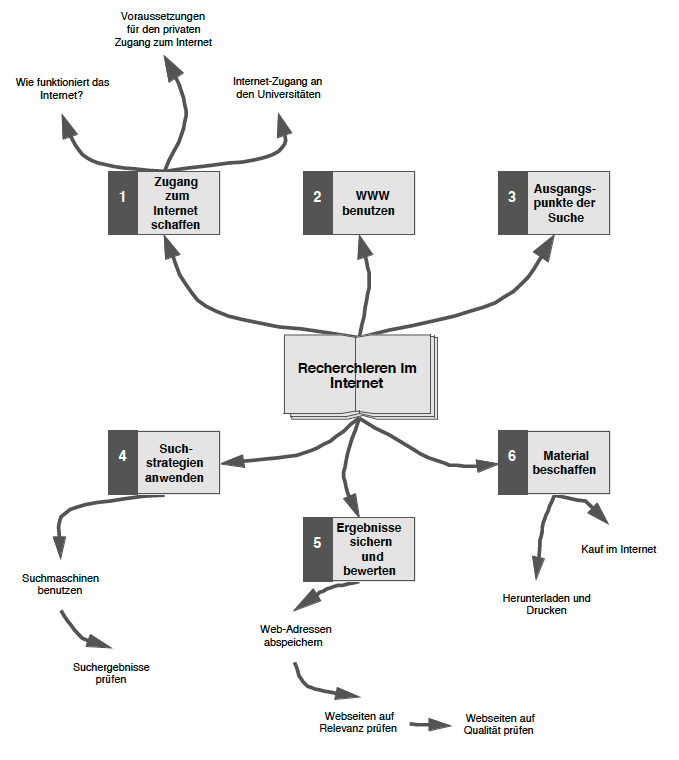
\includegraphics{images/recherchieren-internet-min} 

}

\caption{Recherchieren im Internet (Überblick)}\label{fig:unnamed-chunk-11}
\end{figure}

Mit diesem Kapitel führen wir das Kapitel „Recherchieren`` fort --
hinein ins Internet und die Online-Recherche. Manchen Fundorten für
Materialien werden Sie hier wiederbegegnen, manche Quellen sind jedoch
für das Internet spezifisch und nur über das Netz zugänglich. Die
Informationssuche ist -- nach der E-Mail (siehe Kapitel „Kooperieren``)
-- die wichtigste Nutzungsart des Internets. Zu praktisch jedem Thema
kann man im Internet eine Fülle von Informationen finden, meist zu viel
als zu wenig. Die Fertigkeit, das Internet für wissenschaftliches
Arbeiten zu nutzen, besteht daher weniger darin, etwas zu finden,
sondern darin, mit vernünftigem Aufwand an Zeit und Geld genau das zu
finden, was man braucht, die Qualität des Gefundenen zu bewerten und den
Überblick über die Vielfalt der Quellen zu behalten.

\begin{figure}

{\centering 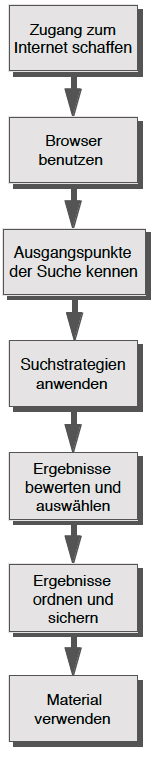
\includegraphics{images/recherchieren-internet-ablauf-min} 

}

\caption{Prozessschritte der Recherche im Internet}\label{fig:unnamed-chunk-12}
\end{figure}

\section{Zugang zum Internet
schaffen}\label{zugang-zum-internet-schaffen}

\subsection{Was ist das Internet?}\label{was-ist-das-internet}

„Internet`` ist der Name eines weltweiten Netzwerkes all jener Computer,
die über das gemeinsame Protokoll TCP/IP (Transmission Control
Protocol/Internet Protocol) miteinander kommunizieren können. Das
Internet ist ein Zusammenschluss von Teil-Netzwerken mit verschiedenen
Betreibern, es gibt daher nicht „den`` Internet-Betreiber. Notwendige
Regulierungen, Standardisierungen, Änderungen usw. werden von weltweiten
Gremien aus Vertretern der Betreiber beschlossen. Durch diese Absprachen
wird sichergestellt, dass trotz der raschen Weiterentwicklung des
Internets die Grundprinzipien erhalten bleiben: einheitliches Protokoll,
Plattformunabhängigkeit usw.

Das Internet entstand aus dem Zusammenschluss verschiedener
spezialisierter Computernetzwerke, die anfangs nur bestimmte Rechner für
bestimmte Zwecke miteinander verbanden. „Internet`` ist die Bezeichnung
für das übergeordnete Netzwerk, das diese Netze mittels eines
gemeinsamen Protokolls verband. Dadurch wurde es möglich, ganz
unterschiedliche Rechner miteinander zu verbinden und eine Reihe von
„Diensten`` zu benutzen. Bis zum Durchbruch des World Wide Web (WWW)
blieb das Internet jedoch ein Netzwerk für die Forschung und von der
breiten Öffentlichkeit unbemerkt. Das WWW wurde 1992 am Europäischen
Kernforschungszentrum CERN eingesetzt, ursprünglich um intern Dokumente
und Berichte zu verwalten und komfortabel abrufen zu können. Der Dienst
wurde an die Internetgemeinde kostenlos weitergegeben, und gab damit den
Anstoß für den weltweiten Siegeszug des WWW und des Internets, dessen
Ende und Auswirkungen noch bei weitem nicht abzusehen sind.

\subsection{Voraussetzungen für den privaten Zugang zum
Internet}\label{voraussetzungen-fur-den-privaten-zugang-zum-internet}

Im Prinzip braucht man für den Zugang zum Internet nicht viel: einen PC,
ein Modem (= MOdulator-DEModulator), eine Leitung für die
Datenübertragung, und einen Provider (= Service- oder Zugangsanbieter).
Praktisch jeder PC ist gut genug für das Internet, es muss kein neuer
und schon gar nicht der teuerste sein.

Bei der Leitung kommt für den privaten Internet-Zugang vor allem die
Telefonleitung in Frage. Sie kann auf verschiedene Weise für die
Datenübertragung genutzt werden:

\begin{itemize}
\tightlist
\item
  analog, d. h. das Modem benutzt das herkömmliche Telefonnetz, um Daten
  in digitaler Form zu übertragen, dzt. mit maximal 56 kbps (= Kilobit
  pro Sekunde)
\item
  digital mit ISDN (Integrated Services Digital Network), einem
  digitalen Verfahren auf der Basis des herkömmlichen Telefonnetzes, das
  pro Telefonanschluss nun zwei Verbindungen gleichzeitig und (etwas)
  höhere Übertragungsraten (64 kbps pro Kanal) ermöglicht.
\item
  digital mit ADSL (Asymmetric Digital Subscriber Line). Dieses
  Verfahren nutzt die Kupferkabel des herkömmlichen Telefonnetzes sehr
  effizient und kann daher preisgünstig angeboten werden. ADSL bietet
  gegenüber Modem- oder ISDN-Verbindungen bis zu zehnmal höhere
  Übertragungsraten. Als weitere Übertragunsgsmedien kommen in Frage:
\item
  (Fernseh-)Kabelnetzwerk: Außer der Telefonleitung wird in
  Ballungsräumen und Großstädten auch die Datenübertragung über das Netz
  des Kabelfernsehens angeboten (über Kupferkoaxialkabel, d.h. ein
  Verbund von mehr Kabeln als den zwei Kupferkabeln der
  Telefonleitungen). Es wird ein eigenes Modem benötigt, das meist vom
  Provider zur Verfügung gestellt wird. Die Datenraten sind hoch, d.h.
  auch für umfangreiche Upload- und Download-Vorgänge geeignet.
\item
  Mobilfunknetz: Über UMTS (Universal Mobile Telecommunications System)
  steht ein drahtloses Verfahren zur Verfügung, dessen Übertragungsraten
  z. B. Videokonferenzen auch im mobilen Einsatz ermöglichen. Derzeit
  wird bereits der nächste Schritt in der mobilen Datenübertragung
  getan, nämlich HSDPA (High Speed Downlink Packet Access) mit
  wesentlich größeren Bandbreiten.
\end{itemize}

Diese verschiedenen Zugangsarten unterscheiden sich zum einen in der
Übertragungsrate, die in Bits (Informationseinheit) pro Sekunde (bps
oder bit/s) angegeben wird (z. B. 1 ISDN-Kanal = 64 kbps = ca. 64 000
bps); zum andern natürlich im Preis. Für den privaten Internet-Zugang
reicht meistens auch die analoge Telefonleitung aus. Einrichtungs- oder
Umstellungskosten fallen dabei -- bis auf die Anschaffung eines Modems
-- weg. Bei ADSL und Fernsehkabel-Zugängen wird oft nach einer
„Flatrate`` abgerechnet, d. h. es wird eine pauschale, fixe Monatsgebühr
verrechnet, unabhängig von der Nutzungsdauer und dem Datenvolumen (in
den Grenzen des „fair use``). „Flatrate`` ist daher für „Dauersurfer``
empfehlenswert.

Schwieriger ist die Wahl des Providers, wenn sie nicht schon durch die
Art der Übertragung festgelegt wird. Ein Provider stellt Internet-Zugang
und -Dienste für seine Kunden zur Verfügung. Seine Infrastruktur
verbindet die Computer der Kunden miteinander und -- was heute viel
wichtiger ist -- mit der „Welt`` des Internets. Die Preise für den
Internet-Zugang sind nur schwer miteinander vergleichbar, denn a) wird
häufig der Internet-Zugang im Paket mit anderen Dienstleistungen (wie
Mobil- und/oder Festnetztelefonie) angeboten, und b) sind die
Abrechnungsmodalitäten und Zusatzleistungen sehr vielfältig. Wir können
daher nur ein paar Anhaltspunkte für die Wahl des Providers liefern. Zum
Teil sind das Fragen, die man selten stellt, weil man zuerst nur auf den
Preis achtet:

\begin{itemize}
\tightlist
\item
  „Gateway`` zum Internet: welche Kapazität? Die Anbindung des Providers
  an das Internet kann zum Nadelöhr für die Kunden werden. So nützen die
  großzügigen Übertragungsraten innerhalb z. B. eines regional
  begrenzten Kabelfernsehnetzes wenig, wenn die Leitung des Anbieters
  nach außen zu schwach ist.
\item
  Datenübertragungskosten: nach Zeit, nach Datenmenge oder pauschal
  (flat rate)? (Diese Kosten sind unabhängig von den allfälligen
  Telefonkosten, die ja nicht der Provider einhebt, sondern die
  Telekommunikationsgesellschaft - falls für den Internetzugang das
  Telefonnetzwerk genutzt wird)
\item
  Was wird zusätzlich zu den Internet-Diensten (E-Mail, WWW) angeboten
  (z. B. mehrere E-Mail-Adressen, Speicherplatz für die eigene Homepage,
  FTP, Telnet)?
\item
  Wie zuverlässig ist der Provider? Wie funktioniert der technische
  Support? Hat er einen effizienten Spam-Filter? funktioniert die
  Abrechnung reibungslos und korrekt? Hier ist man meistens auf
  Erfahrungen anderer Benutzer angewiesen.
\end{itemize}

\subsection{Internet-Zugang an den
Universitäten}\label{internet-zugang-an-den-universitaten}

Universitäten bieten PC-Benutzerräume für Studierende mit Rechnern, die
ans Internet angeschlossen sind. So können auch Studierende ohne eigenen
Computer die Internetdienste nutzen. Abgesehen davon, dass der Andrang
in diesen öffentlichen Benutzerräumen meist groß ist, denn das Angebot
an Computerarbeitsplätzen hinkt der Nachfrage ständig hinterher, müssen
Sie einige Dinge berücksichtigen, wenn Sie an ständig wechselnden
Computern arbeiten müssen:

\begin{itemize}
\tightlist
\item
  Die Verwaltung Ihrer E-Mails ist schwierig, wenn die Nachrichten bei
  jeder Sitzung auf den lokalen Rechner übertragen werden. Dann können
  Sie nie in alten E- Mails suchen und verlieren leicht die Übersicht
  darüber, was Sie schon beantwortet oder weitergeleitet haben. Eine
  einfache und unkomplizierte Lösung dafür liegt in der Benutzung von
  Web-Zugängen zu Ihrem E-Mail-Server, wie ihn viele Free- Mailer und
  Universitäten bieten. Über Ihren Browser können Sie dann von überall
  her auf Ihre Nachrichten zugreifen. Allerdings bieten alle
  Internet-Provider nur einen begrenzten Platz für die Speicherung Ihrer
  E-Mails. Wenn Sie diesen Speicherplatz ausgeschöpft haben, können Sie
  erst wieder E-Mails erhalten, wenn Sie alte (und vor allem
  umfangreiche) Nachrichten gelöscht haben.
\item
  Ihre im Web-Browser angelegten „Lesezeichen`` (siehe „Web-Adressen
  abspeichern``) werden im Normalfall lokal gespeichert. Benutzer-PCs an
  Universitäten können allerdings so konfiguriert sein, dass die
  Lesezeichen automatisch auf einem Server -- in Ihrem
  Benutzervrezeichnis -- abgelegt werden und daher von jedem Rechner aus
  zugänglich sind. Ist das nicht der Fall oder müssen Sie auch zwischen
  anderen, nicht vernetzten PCs wechseln, werden Sie andere Lösungen
  finden müssen: Wenn Sie eine eigene Website (Homepage) haben, können
  Sie Ihre Lesezeichen von Zeit zu Zeit exportieren und als HTML-Datei
  auf Ihrer Website speichern. Dann können Sie zwar von überall her auf
  Ihre Lesezeichen zugreifen, das Anlegen neuer Lesezeichen bleibt aber
  weiterhin auf den PC beschränkt, an dem Sie gerade arbeiten. Einen
  ortsneutralen Zugang ermöglichen jene Anbieter, die sich auf die
  Speicherung von Lesezeichen im Web spezialisiert haben. Ihre Daten
  liegen dann passwortgeschützt im Internet und lassen sich mit der
  Unterstützung einer Software auf Ihrem PC synchronisieren. Da diese
  Dienste per Web- Formular auch die Eintragung von überall her
  erlauben, können Sie von jedem Standort aus auf Ihre Lesezeichen
  sowohl lesend als auch schreibend zugreifen.
\end{itemize}

\section{WWW benutzen}\label{www-benutzen}

Um ins World Wide Web -- WWW -- zu gelangen, benötigt man neben dem
Internet-Zugang auch ein Programm auf dem lokalen PC, einen sogenannten
„Browser`` (von to browse = blättern, schmökern). Die folgende Tabelle
zeigt die wichtigsten Funktionen, die ein Browser -- unabhängig davon,
welches Produkt Sie verwenden, haben sollte:

\begin{longtable}[]{@{}lll@{}}
\caption{\textbf{\label{tab:browser-benutzen} Broswer
benutzen}}\tabularnewline
\toprule
\begin{minipage}[b]{0.31\columnwidth}\raggedright\strut
Sie verwenden die Funktion\strut
\end{minipage} & \begin{minipage}[b]{0.27\columnwidth}\raggedright\strut
und können damit\ldots{}\strut
\end{minipage} & \begin{minipage}[b]{0.33\columnwidth}\raggedright\strut
Anmerkung\strut
\end{minipage}\tabularnewline
\midrule
\endfirsthead
\toprule
\begin{minipage}[b]{0.31\columnwidth}\raggedright\strut
Sie verwenden die Funktion\strut
\end{minipage} & \begin{minipage}[b]{0.27\columnwidth}\raggedright\strut
und können damit\ldots{}\strut
\end{minipage} & \begin{minipage}[b]{0.33\columnwidth}\raggedright\strut
Anmerkung\strut
\end{minipage}\tabularnewline
\midrule
\endhead
\begin{minipage}[t]{0.31\columnwidth}\raggedright\strut
Einstellungen, Optionen \ldots{} \vspace{5mm}\strut
\end{minipage} & \begin{minipage}[t]{0.27\columnwidth}\raggedright\strut
Voreinstellungen für Verbindung, Erscheinungsbild, Sicherheit, Verhalten
des Browsers definieren \vspace{5mm}\strut
\end{minipage} & \begin{minipage}[t]{0.33\columnwidth}\raggedright\strut
\strut
\end{minipage}\tabularnewline
\begin{minipage}[t]{0.31\columnwidth}\raggedright\strut
eine Webadresse (URL) eingeben \vspace{5mm}\strut
\end{minipage} & \begin{minipage}[t]{0.27\columnwidth}\raggedright\strut
die betreffende Webseite abrufen\strut
\end{minipage} & \begin{minipage}[t]{0.33\columnwidth}\raggedright\strut
\strut
\end{minipage}\tabularnewline
\begin{minipage}[t]{0.31\columnwidth}\raggedright\strut
Blättern \vspace{5mm}\strut
\end{minipage} & \begin{minipage}[t]{0.27\columnwidth}\raggedright\strut
zwischen den bereits aufgerufenen Seiten wechseln \vspace{5mm}\strut
\end{minipage} & \begin{minipage}[t]{0.33\columnwidth}\raggedright\strut
schneller als erneutes Laden, da im „Cache`` (lokal) gespeichert
\vspace{5mm}\strut
\end{minipage}\tabularnewline
\begin{minipage}[t]{0.31\columnwidth}\raggedright\strut
Home (Startseite) \vspace{5mm}\strut
\end{minipage} & \begin{minipage}[t]{0.27\columnwidth}\raggedright\strut
zu der von Ihnen definierten Startseite zurückkehren \vspace{5mm}\strut
\end{minipage} & \begin{minipage}[t]{0.33\columnwidth}\raggedright\strut
günstig als Startseite: die bevorzugte Suchmaschine oder eine aktuelle
Nachrichtenseite\vspace{5mm}\strut
\end{minipage}\tabularnewline
\begin{minipage}[t]{0.31\columnwidth}\raggedright\strut
„history`` (Liste der bereits aufgerufenen Seiten) \vspace{5mm}\strut
\end{minipage} & \begin{minipage}[t]{0.27\columnwidth}\raggedright\strut
zwischen allen bereits aufgerufenen Seiten wechseln \vspace{5mm}\strut
\end{minipage} & \begin{minipage}[t]{0.33\columnwidth}\raggedright\strut
schneller als erneutes Laden, da im „Cache`` (lokal) gespeichert
\vspace{5mm}\strut
\end{minipage}\tabularnewline
\begin{minipage}[t]{0.31\columnwidth}\raggedright\strut
„reload`` (erneut laden) \vspace{5mm}\strut
\end{minipage} & \begin{minipage}[t]{0.27\columnwidth}\raggedright\strut
die aktuelle Webseite nochmals abrufen \vspace{5mm}\strut
\end{minipage} & \begin{minipage}[t]{0.33\columnwidth}\raggedright\strut
z. B. bei Übertragungsfehlern oder zwischenzeitlichen Änderungen
\vspace{5mm}\strut
\end{minipage}\tabularnewline
\begin{minipage}[t]{0.31\columnwidth}\raggedright\strut
Lesezeichen oder Favoriten \vspace{5mm}\strut
\end{minipage} & \begin{minipage}[t]{0.27\columnwidth}\raggedright\strut
Webadressen speichern \vspace{5mm}\strut
\end{minipage} & \begin{minipage}[t]{0.33\columnwidth}\raggedright\strut
s. unten \vspace{5mm}\strut
\end{minipage}\tabularnewline
\begin{minipage}[t]{0.31\columnwidth}\raggedright\strut
Drucken \vspace{5mm}\strut
\end{minipage} & \begin{minipage}[t]{0.27\columnwidth}\raggedright\strut
um Seiten (oder „Frames``) auszudrucken \vspace{5mm}\strut
\end{minipage} & \begin{minipage}[t]{0.33\columnwidth}\raggedright\strut
\strut
\end{minipage}\tabularnewline
\bottomrule
\end{longtable}

Die Grundfunktion des Browsers ist es, Webseiten HTML-Dokumente, HTML =
Hypertext Markup Language) mitsamt den eingebauten Verknüpfungen
(Hyperlinks) auf dem Bildschirm darzustellen und die vom Benutzer
eingegebenen oder angeklickten Web-Adressen (URL = uniform resource
locator) an das Interent weiterzuleiten.

Die Darstellung von Webseiten umfasst auch die Darstellung von „Frames``
(Rahmen), den vordefinierten Unterteilungen von Webseiten. Frames werden
meist dazu verwendet, um Navigationselemente und Menüs einer Website (=
zusammengehörige Sammlung von Webseiten) in einem eigenen,
gleichbleibenden Bereich des Browser-Fensters zusammenzufassen.

Weitere Funktionen, wie z. B. die Wiedergabe von Ton, Animationen oder
Video, sind entweder (bei neuen Versionen) bereits im Browser integriert
oder müssen als Zusatzprogramme (Plug-Ins) installiert werden. Die
meisten Plug-Ins können aus dem Internet heruntergeladen und einfach
installiert werden. Sind sie einmal installiert, erkennt der Browser
automatisch, wann welches Zusatzprogramm aufgerufen werden muss.
Plug-Ins erweitern die Darstellungsmöglichkeiten der Browser um weitere,
meist herstellerabhängige Dateiformate oder andere spezielle Funktionen
wie z. B. das Navigieren in 3D-Welten. Websites, die solche
Multimedia-Elemente enthalten, bieten meistens auch einen Link auf die
Bezugsquelle der zum Abspielen notwendigen Zusatzprogramme.

\section{Ausgangspunkte der Suche}\label{ausgangspunkte-der-suche}

Um die Recherche im Internet beginnen zu können, brauchen Sie einen
ersten Anhalts- oder Ausgangspunkt. Das könnten sein

\begin{itemize}
\tightlist
\item
  \emph{Suchmaschinen}: Zugriff auf zahlreiche Webseiten, die
  automatisch von der Suchmaschine erfasst werden; die Webseiten sind
  nicht nach Qualität selektiert oder bewertet, d. h. man erhält im
  Normalfall sehr viele Ergebnisse, die man selbst prüfen muss.
  Suchmaschinen unterscheiden sich nach der Art und Menge der Webseiten,
  die sie erfassen. Um eine halbwegs vollständige Übersicht über die
  Webseiten zu einem Thema zu erhalten, sollte man daher mit mindestens
  zwei Suchmaschinen arbeiten. Dafür gibt es auch sogenannte
\item
  \emph{Metasuchmaschinen}, die für eine Suche automatisch mehrere
  Suchmaschinen heranziehen.
\item
  \emph{Spezielle Suchmaschinen}, wie. z.B. das deutsche
  Forschungsportal, mit einem beschränkten, dafür geprüften Suchraum
  (hier Universitäten und wissenschaftliche Organisationen). Das
  Forschungsportal erfasst im gegensatz zu den meisten anderen
  Suchmaschinen auch dynamische Webseiten, das sind solche, die erst bei
  Aufruf aus Datenbanken generiert werden.
\item
  \emph{Wiki}, auch WikiWiki und WikiWeb genannt, ist eine im World Wide
  Web verfügbare Seitensammlung, die von den Benutzern nicht nur
  gelesen, sondern auch online geändert werden kann. Wikis ähneln damit
  Content Management Systemen. Der Name stammt von wikiwiki, dem
  hawaiianischen Wort für „schnell``. Wie bei Hypertexten üblich, sind
  die einzelnen Seiten und Artikel eines Wikis durch Querverweise
  (Links) miteinander verbunden. Dazu gibt es in der Regel eine
  Bearbeitungsfunktion, die ein Eingabefenster öffnet, in dem der Text
  des Artikels bearbeitet werden kann. Das weltweit größte Wiki ist die
  Wikipedia, die in mehreren Sprachen von ehrenamtlichen Autoren
  verfasst und ständig erweitert wird. \url{http://de.wikipedia.org/}
\item
  \emph{Kataloge}: vorgefertigte und (meist) selektierte Sammlungen von
  Links zu den verschiedensten Themen. Viele Suchmaschinen bieten
  zugleich auch einen Katalog oder Index, der hierarchisch von
  allgemeinen zu spezielleren Themen führt. Zum Einstieg in ein Thema
  sind solche Kataloge gut geeignet, allerdings sind sie selten
  spezifisch genug.
\item
  \emph{Linksammlungen und ``Portale''}: fach- oder gar
  themenspezifische Sammlungen von Dokumenten und Hyperlinks, die von
  Institutionen, Projekten, manchmal auch von Privatpersonen
  zusammengestellt wurden. Gute Portale enthalten bereits einen Großteil
  der für ein Thema oder Fachgebiet relevanten Links. Wenn eine
  Linksammlung allerdings in einer einmaligen Aktion angelegt wurde und
  nicht dauernd gewartet wird, veraltet sie sehr schnell, d.h. viele
  Links funktionieren nicht mehr. Ein weiteres Problem ist, dass diese
  Sammlungen natürlich auch keinen Anspruch auf Vollständigkeit erheben
  können. Eine zusätzliche Suche ist auf jeden Fall ratsam.
\item
  \emph{Suche in einzelnen Websites bzw. Datenbanken}: Von der
  „offenen`` Suche im gesamten Internet unterscheiden wir die
  „geschlossene`` in einer bestimmten Website bzw. Datenbank. Das
  betrifft z. B. Bibliotheken, Versandbuchhandlungen, das Verzeichnis
  lieferbarer Bücher, Zeitschriften-Indizes usw. Wenn man einmal die
  Web-Adressen der wichtigsten Fundorte dieser Art gefunden hat, wird
  man sie immer wieder beim Bibliografieren verwenden.
\end{itemize}

\section{Suchstrategien anwenden}\label{suchstrategien-anwenden}

In diesem Abschnitt geht es um die „Kunst``, mit Suchmaschinen so zu
arbeiten, dass man auch wirklich findet, was man sucht. Das ist
keineswegs trivial: Im WWW finden sich zu praktisch allen Stichworten
(v. a. englischen) viele bis sehr viele Seiten. Es ist unmöglich, alle
diese Ergebnisse durchzusehen. Daher wird man von vornherein versuchen,
eine Abfrage so genau zu formulieren, dass wenige, dafür aber passende
Treffer erzielt werden.

\subsection{Suchmaschinen benutzen}\label{suchmaschinen-benutzen}

Suchmaschinen sind riesige Datenbanken. Sie werden ständig automatisch
aktualisiert und erweitert. Eigenständige Programme (Crawler, Robots
oder Spider genannt) durchsuchen weltweit die Web-Server. Sie finden auf
einer Seite, die sie schon indiziert haben, neue Verknüfungen, die sie
dann regelmäßig nach weiteren bzw. aktualisierten Informationen
durchsuchen. Alle Wörter bis auf die häufigsten (sog. „Stopwörter``, z.
B. und, der, die, das, \ldots{}) werden in einer Liste gespeichert, auf
der die Suchanfrage durchgeführt wird. Jedes Wort in der Liste ist mit
denjenigen Internetseiten verknüpft, auf denen der Suchbegriff
auftaucht.

Die Qualität von Suchmaschinen hängt wesentlich davon ab, wie oft und
wie gründlich das WWW durchsucht wird (Abdeckungsgrad). Außerdem spielt
die Relevanz der Suchergebnisse eine Rolle, die sich vor allem in der
Sortierung („Ranking``) der Suchergebnisse ausdrückt. Die relevanten
Treffer sollten sich am Anfang der Ergebnisliste, d. h. unter den ersten
10 bis 20 Treffern finden. Wortorientierte, statistische Verfahren
speichern beispielsweise, wie oft ein bestimmter Begriff auf einer
bestimmten Seite auftaucht. Je häufiger ein Suchbegriff im Dokument, im
Titel oder in den Überschriften auftaucht, desto zentraler scheint das
Dokument bezüglich eines Suchbegriffs, und desto weiter oben rangiert es
in der Liste der Ergebnisse.

Dieses Verfahren ist mangelhaft, da es die Vernetzung der Internetseiten
untereinander außer Acht lässt. Neuere Analyseverfahren untersuchen z.
B., wie viele Links von einer bestimmten Seite auf eine andere Seite
führen. Je mehr Links auf eine Seite zeigen, desto „wichtiger`` ist sie.
Es wird dabei auch beachtet, mit welchen Wörtern auf eine Seite
verwiesen wird. Die Rangordnung wird also nicht mehr über das Thema
hergestellt, sondern über die Popularität einer Seite. Der Nachteil
solcher Verfahren ist, dass eine wichtige, aber „unpopuläre`` Website
kein gutes Ranking erhält. Das erste, was man von Suchmaschinen sieht,
ist ein Eingabefenster für die Suchbegriffe und die Schaltfläche, mit
der die Suche gestartet wird. Die Suche nach einzelnen Stichworten ist
jedoch wenig zielführend. Meistens ergibt sie viele Treffer. Darunter
befinden sich auch zahlreiche Webseiten, auf denen das Stichwort nur
zufällig oder in ganz anderen Zusammenhängen vorkommt. Selbst das
„Ranking`` (s. oben) durch die Suchmaschine ergibt noch Hunderte oder
Tausende möglicherweise relevanter Treffer.

Suchmaschinen können aber wesentlich mehr, als bloß nach einem einzelnen
Begriff zu suchen. Nicht immer sind alle der in der folgenden Tabelle
aufgelisteten Funktionen und Operatoren verfügbar. Vor dem Einsatz einer
Suchmaschine sollte man daher in der Online-Hilfe nachsehen, um Art und
Verwendung von Suchoperatoren kennenzulernen. Die Boole'schen``
(logischen) Operatoren AND, OR und NOT finden sich, wenn überhaupt,
meist erst bei der Eingabemaske für „Fortgeschrittene`` (unter
Bezeichnungen wie advanced search, erweiterte Suche, Profi-Suche u.
dgl.)

\begin{longtable}[]{@{}lll@{}}
\caption{\textbf{\label{tab:suchmaschinen} Mit Suchmaschinen
arbeiten}}\tabularnewline
\toprule
\begin{minipage}[b]{0.31\columnwidth}\raggedright\strut
Sie verwenden \ldots{}\strut
\end{minipage} & \begin{minipage}[b]{0.27\columnwidth}\raggedright\strut
Das bedeutet\ldots{}\strut
\end{minipage} & \begin{minipage}[b]{0.33\columnwidth}\raggedright\strut
Beispiel\strut
\end{minipage}\tabularnewline
\midrule
\endfirsthead
\toprule
\begin{minipage}[b]{0.31\columnwidth}\raggedright\strut
Sie verwenden \ldots{}\strut
\end{minipage} & \begin{minipage}[b]{0.27\columnwidth}\raggedright\strut
Das bedeutet\ldots{}\strut
\end{minipage} & \begin{minipage}[b]{0.33\columnwidth}\raggedright\strut
Beispiel\strut
\end{minipage}\tabularnewline
\midrule
\endhead
\begin{minipage}[t]{0.31\columnwidth}\raggedright\strut
Suche nach Zeichenketten (meist in Anführungszeichen eingeschlossen)
\vspace{5mm}\strut
\end{minipage} & \begin{minipage}[t]{0.27\columnwidth}\raggedright\strut
mehrere Begriffe werden als einer behandelt, die komplette Phrase wird
wörtlich gesucht\vspace{5mm}\strut
\end{minipage} & \begin{minipage}[t]{0.33\columnwidth}\raggedright\strut
„virtual world``; „ich hab genug`` usw. \vspace{5mm}\strut
\end{minipage}\tabularnewline
\begin{minipage}[t]{0.31\columnwidth}\raggedright\strut
den Operator OR bzw. Aneinanderreihung von Suchbegriffen
\^{}1{[}Überprüfen Sie, z. B. anhand der Online-Hilfe, welche
Voreinstellung für Ihre Suchmaschine gilt{]}\vspace{5mm}\strut
\end{minipage} & \begin{minipage}[t]{0.27\columnwidth}\raggedright\strut
Einer der beiden Begriffe oder beide sollen auf der Webseite vorkommen
\vspace{5mm}\strut
\end{minipage} & \begin{minipage}[t]{0.33\columnwidth}\raggedright\strut
virtual world oder virtual OR world = getrennte Suche nach „virtual``
und „world`` \vspace{5mm}\strut
\end{minipage}\tabularnewline
\begin{minipage}[t]{0.31\columnwidth}\raggedright\strut
den Operator AND bzw. Aneinanderreihung von Suchbegriffen
\^{}1{[}Überprüfen Sie, z. B. anhand der Online-Hilfe, welche
Voreinstellung für Ihre Suchmaschine gilt{]} \vspace{5mm}\strut
\end{minipage} & \begin{minipage}[t]{0.27\columnwidth}\raggedright\strut
Beide Suchbegriffe müssen auf der Webseite vorkommen \vspace{5mm}\strut
\end{minipage} & \begin{minipage}[t]{0.33\columnwidth}\raggedright\strut
virtual world oder virtual AND world = gemeinsame Suche nach „virtual``
and „world`` \vspace{5mm}\strut
\end{minipage}\tabularnewline
\begin{minipage}[t]{0.31\columnwidth}\raggedright\strut
„wild cards`` (Platzhalter), z. B. * oder ? \vspace{5mm}\strut
\end{minipage} & \begin{minipage}[t]{0.27\columnwidth}\raggedright\strut
an dieser Stelle im Suchbegriff dürfen beliebige Zeichen erscheinen
\vspace{5mm}\strut
\end{minipage} & \begin{minipage}[t]{0.33\columnwidth}\raggedright\strut
interpassiv* = Suche nach interpassiv/e/er/en, Interpassivität usw.
\vspace{5mm}\strut
\end{minipage}\tabularnewline
\begin{minipage}[t]{0.31\columnwidth}\raggedright\strut
Einschränkung auf bestimmte Sprache \vspace{5mm}\strut
\end{minipage} & \begin{minipage}[t]{0.27\columnwidth}\raggedright\strut
nur Webseiten in der angegebenen Sprache werden angezeigt
\vspace{5mm}\strut
\end{minipage} & \begin{minipage}[t]{0.33\columnwidth}\raggedright\strut
„interpassiv*`` in beliebiger Sprache = 120 Treffer, in Deutsch = 33
Treffer \vspace{5mm}\strut
\end{minipage}\tabularnewline
\begin{minipage}[t]{0.31\columnwidth}\raggedright\strut
den Operator NEAR (nahe) = Kontextsuche \vspace{5mm}\strut
\end{minipage} & \begin{minipage}[t]{0.27\columnwidth}\raggedright\strut
zwischen den beiden Suchbegriffen darf nur eine bestimmte Anzahl Worte
stehen; ein Suchbegriff muss im Umfeld eines anderen auftreten
\vspace{5mm}\strut
\end{minipage} & \begin{minipage}[t]{0.33\columnwidth}\raggedright\strut
agent NEAR „virtual character`` = agent soll max. 10 Wörter (AltaVista)
von „virtual character`` entfernt auftreten \vspace{5mm}\strut
\end{minipage}\tabularnewline
\begin{minipage}[t]{0.31\columnwidth}\raggedright\strut
den Operator NOT vor einem Suchbegriff \vspace{5mm}\strut
\end{minipage} & \begin{minipage}[t]{0.27\columnwidth}\raggedright\strut
dieser Suchbegriff soll ausgeschlossen werden; günstig, wenn eine
häufige Zusammensetzung unerwünscht ist \vspace{5mm}\strut
\end{minipage} & \begin{minipage}[t]{0.33\columnwidth}\raggedright\strut
frame AND NOT picture = Suche nach „frame``, aber nicht in der
Zusammensetzung „picture frame`` (Bilderrahmen) \vspace{5mm}\strut
\end{minipage}\tabularnewline
\begin{minipage}[t]{0.31\columnwidth}\raggedright\strut
Klammern in komplexen Suchabfragen \vspace{5mm}\strut
\end{minipage} & \begin{minipage}[t]{0.27\columnwidth}\raggedright\strut
Bedingungen in Klammern werden zuerst ausgewertet; vorgegebene Priorität
der Operatoren (AND vor OR) wird umgangen \vspace{5mm}\strut
\end{minipage} & \begin{minipage}[t]{0.33\columnwidth}\raggedright\strut
(kalb OR kuh) AND schwarz = Webseiten mit kalb AND schwarz sowie Seiten
mit kuh AND schwarz. kalb OR kuh AND schwarz = Seiten mit kuh AND
schwarz sowie Seiten mit kalb. \vspace{5mm}\strut
\end{minipage}\tabularnewline
\begin{minipage}[t]{0.31\columnwidth}\raggedright\strut
den Operator „+`` unmittelbar vor einem Suchbegriff \vspace{5mm}\strut
\end{minipage} & \begin{minipage}[t]{0.27\columnwidth}\raggedright\strut
Das Wort \emph{muss} auf der Webseite vorkommen \vspace{5mm}\strut
\end{minipage} & \begin{minipage}[t]{0.33\columnwidth}\raggedright\strut
berlin +immobilie = Suche nach Seiten zu Berlin, auf denen das Wort
„Immobilie`` vorkommt \vspace{5mm}\strut
\end{minipage}\tabularnewline
\begin{minipage}[t]{0.31\columnwidth}\raggedright\strut
den Operator „-`` unmittelbar vor einem Suchbegriff \vspace{5mm}\strut
\end{minipage} & \begin{minipage}[t]{0.27\columnwidth}\raggedright\strut
Das Wort \emph{darf} auf der Webseite \emph{nicht} vorkommen
\vspace{5mm}\strut
\end{minipage} & \begin{minipage}[t]{0.33\columnwidth}\raggedright\strut
berlin -briefmarke = Suche nach Seiten zu Berlin, auf denen das Wort
„Briefmarke`` nicht vorkommt \vspace{5mm}\strut
\end{minipage}\tabularnewline
\bottomrule
\end{longtable}

Die Gefahr bei der Suche im WWW ist heute schon längst nicht mehr, dass
Sie nichts finden, sondern dass Sie viel zu viel finden: Sie müssen sich
bei den meisten Suchmaschinen schon sehr anstrengen, um sich einen
Suchbegriff auszudenken, für den überhaupt keine Treffer erzielt werden.
Heute geht es eher darum, möglichst das Wichtige oder Richtige aus den
vielen Ergebnissen herauszufiltern. Deshalb ist die Bedeutung der
Metasuchmaschinen zurückgegangen. Sie liefern auf jeden Fall eine höhere
Trefferquote als eine einzelne Suchmaschine, doch eine Sortierung der
Treffer ist nicht möglich (da diese ja auf den Kriterien der einzelnen
Suchmaschinen beruht). Umfangreiche Ergebnislisten von Metasuchmaschinen
sind daher unübersichtlich oder sogar unbrauchbar. Sinnvoll ist ihre
Verwendung dagegen bei der Suche nach sehr seltenen Suchbegriffen.

\subsection{Suchergebnisse prüfen}\label{suchergebnisse-prufen}

Die Trefferliste ist geordnet nach dem Prinzip „best first``, d. h. die
Ergebnisse, die nach dem Verfahren der Suchmaschine den Suchkriterien am
meisten entsprechen, erscheinen als erste. Ein kurzer Blick auf diese
ersten Fundstellen kann Ihnen daher schon sagen, ob Sie mit Ihrer
Suchabfrage richtig liegen. Wenn hier schon Treffer auftauchen, die mit
Ihrer Abfrage anscheinend nichts zu tun haben, so ist eine andere
Suchstrategie angebracht. Sie müssen herausfinden, wie Sie die
unerwünschten Fundstellen ausschließen können. Das kann geschehen durch

\begin{itemize}
\tightlist
\item
  einen anderen Suchbegriff (Synonym, unter- oder übergeordneter
  Begriff, Phrase \ldots{})
\item
  eine komplexe Suchabfrage, mit (Boole'schen) Operatoren verknüpft,
  siehe Aktionstabelle oben.
\end{itemize}

Das „best first``-Prinzip kann Ihnen aber auch eine mühsame weitere
Einschränkung des Suchraumes ersparen. Wenn Sie -- bei einer nicht allzu
großen Menge von Ergebnissen (bis maximal 100) -- die ersten zehn
Treffer aufrufen, können Sie feststellen, ob Sie mit Ihrer Suche „ins
Schwarze`` getroffen haben. Das wären z. B. Seiten, die als Startseiten
und Linksammlungen zum Thema konzipiert sind, und von denen aus Sie
gleich themenspezifisch weitere Websites erschließen können. Wenn sich
darüber hinaus in so einer Linksammlung die selben Adressen finden, die
auch in der Trefferliste erscheinen, so können Sie schon ziemlich sicher
sein, dass Sie das Gebiet bereits einigermaßen erschlossen haben.

Trotzdem sollten Sie auch die weiter unten gereihten Treffer überfliegen
oder stichprobenartig prüfen. Wenn die letzten noch (beinahe) ebenso
relevant sind wie die ersten und die Gesamtzahl der Treffer zu hoch ist,
um alle einzeln aufzurufen, sollten Sie doch noch engere und speziellere
Suchbegriffe probieren

\section{Ergebnisse sichern und
bewerten}\label{ergebnisse-sichern-und-bewerten}

Nehmen wir an, Sie haben mit der Suche ein rundes Dutzend relevanter und
vielversprechender Treffer erzielt. Sie müssen nun * sicherstellen, dass
Sie sie identifizieren und wiederfinden können, und * jede Fundstelle
sichten und auf Qualität und Relevanz für Ihr Thema untersuchen

\subsection{Web-Adressen abspeichern}\label{web-adressen-abspeichern}

Internet-Browser stellen Funktionen („Lesezeichen`` oder „Favoriten`` in
den meistverwendeten Browsern) zur Verfügung, mit denen Sie selbst
Sammlungen von Links anlegen können. Diese können dann direkt aus dem
Browser heraus aufgerufen werden.

Um ein solches Lesezeichen anzulegen, muss die entsprechende Seite nicht
einmal geöffnet werden. Es ist auch möglich, einen Hyperlink auf einer
Webseite auf diese Weise abzuspeichern. Diese Vorgangsweise genügt für
die Sicherung der Ergebnisse im ersten Durchgang. Nach der Sichtung und
Prüfung müssen diese Lesezeichen (oder Favoriten) jedoch weiter
bearbeitet werden.

Web-Adressen sind schnell gespeichert -- die Technik ist nicht das
Problem, sondern, wie so oft, die Organisation. Endlose Listen von
Lesezeichen/Favoriten werden schnell unübersichtlich und damit wertlos.
Je nach dem verwendeten Browser können und sollten Sie * den
Lesezeichen/Favoriten aussagekräftige Namen geben, * sie mit Anmerkungen
kommentieren, * sie in themenspezifischen Ordnern zusammenfassen und *
regelmäßig prüfen, ob die Links noch korrekt sind.

Die Verwaltung von gespeicherten Web-Adressen ist bei den gängigen
Browsern nur unbefriedigend gelöst. Schwierig wird sie vor allem, wenn
man die eigenen Lesezeichen von verschiedenen Rechnern oder mit
unterschiedlichen Browsern verwenden will. Es gibt Dienstprogramme, die
die Verwaltung erleichtern. Neben dem Abspeichern und Kommentieren
erlauben sie das Prüfen der Links und das Konvertieren für andere
Browser. Manche Provider bieten die Verwaltung der Lesezeichen im WWW
an. Dann ist es möglich, über den Web-Browser von einem beliebigen
Rechner aus auf die Lesezeichen zuzugreifen.

\subsection{Webseiten auf Relevanz
prüfen}\label{webseiten-auf-relevanz-prufen}

Nun werden diese „roh`` gesammelten Hyperlinks der Reihe nach aufgerufen
und geprüft, und zwar auf ihre Relevanz und ihre Qualität. Für diese
Prüfung empfiehlt es sich, systematisch und nach Plan vorzugehen, da man
sonst in Gefahr ist, in zielloses Surfen und Blättern zu geraten, immer
noch mehr Hyperlinks zu folgen und immer neue Fundstellen zu öffnen,
ohne ein Bild davon zu haben, was man bereits gefunden hat. Es kann ja
durchaus sinnvoll und notwendig sein, den Verweisen auf einer mit der
Suchmaschine gefundenen Seite nachzugehen, aber es ist ratsam, das in
einem späteren Durchgang zu machen.

\begin{longtable}[]{@{}lll@{}}
\caption{\textbf{\label{tab:urls} Beginn von URLs}}\tabularnewline
\toprule
\begin{minipage}[b]{0.31\columnwidth}\raggedright\strut
Die Web-Adresse beginnt mit\ldots{}\strut
\end{minipage} & \begin{minipage}[b]{0.27\columnwidth}\raggedright\strut
Das heißt\ldots{}\strut
\end{minipage} & \begin{minipage}[b]{0.33\columnwidth}\raggedright\strut
Es handelt sich um\ldots{}\strut
\end{minipage}\tabularnewline
\midrule
\endfirsthead
\toprule
\begin{minipage}[b]{0.31\columnwidth}\raggedright\strut
Die Web-Adresse beginnt mit\ldots{}\strut
\end{minipage} & \begin{minipage}[b]{0.27\columnwidth}\raggedright\strut
Das heißt\ldots{}\strut
\end{minipage} & \begin{minipage}[b]{0.33\columnwidth}\raggedright\strut
Es handelt sich um\ldots{}\strut
\end{minipage}\tabularnewline
\midrule
\endhead
\begin{minipage}[t]{0.31\columnwidth}\raggedright\strut
\url{http://} \vspace{5mm}\strut
\end{minipage} & \begin{minipage}[t]{0.27\columnwidth}\raggedright\strut
HyperText Transfer Protocol \vspace{5mm}\strut
\end{minipage} & \begin{minipage}[t]{0.33\columnwidth}\raggedright\strut
HTML-Seiten (häufigster Fall im WWW) \vspace{5mm}\strut
\end{minipage}\tabularnewline
\begin{minipage}[t]{0.31\columnwidth}\raggedright\strut
\url{ftp://} \vspace{5mm}\strut
\end{minipage} & \begin{minipage}[t]{0.27\columnwidth}\raggedright\strut
File Transfer Protocol \vspace{5mm}\strut
\end{minipage} & \begin{minipage}[t]{0.33\columnwidth}\raggedright\strut
Dateien/Programme zum Herunterladen \vspace{5mm}\strut
\end{minipage}\tabularnewline
\begin{minipage}[t]{0.31\columnwidth}\raggedright\strut
\url{File://} \vspace{5mm}\strut
\end{minipage} & \begin{minipage}[t]{0.27\columnwidth}\raggedright\strut
Datei \vspace{5mm}\strut
\end{minipage} & \begin{minipage}[t]{0.33\columnwidth}\raggedright\strut
Lokale HTML-Dateien (auf Ihrem Rechner) \vspace{5mm}\strut
\end{minipage}\tabularnewline
\bottomrule
\end{longtable}

\begin{longtable}[]{@{}lll@{}}
\caption{\textbf{\label{tab:urls2} Ende von URLs}}\tabularnewline
\toprule
\begin{minipage}[b]{0.23\columnwidth}\raggedright\strut
Die Web-Adresse endet mit\ldots{}\strut
\end{minipage} & \begin{minipage}[b]{0.13\columnwidth}\raggedright\strut
Das heißt\ldots{}\strut
\end{minipage} & \begin{minipage}[b]{0.56\columnwidth}\raggedright\strut
Es handelt sich um\ldots{}\strut
\end{minipage}\tabularnewline
\midrule
\endfirsthead
\toprule
\begin{minipage}[b]{0.23\columnwidth}\raggedright\strut
Die Web-Adresse endet mit\ldots{}\strut
\end{minipage} & \begin{minipage}[b]{0.13\columnwidth}\raggedright\strut
Das heißt\ldots{}\strut
\end{minipage} & \begin{minipage}[b]{0.56\columnwidth}\raggedright\strut
Es handelt sich um\ldots{}\strut
\end{minipage}\tabularnewline
\midrule
\endhead
\begin{minipage}[t]{0.23\columnwidth}\raggedright\strut
.de, .ch, .at usw. \vspace{5mm}\strut
\end{minipage} & \begin{minipage}[t]{0.13\columnwidth}\raggedright\strut
Länderkürzel \vspace{5mm}\strut
\end{minipage} & \begin{minipage}[t]{0.56\columnwidth}\raggedright\strut
genormte Länderkürzel; werden national vergeben, sind aber frei
zugänglich \vspace{5mm}\strut
\end{minipage}\tabularnewline
\begin{minipage}[t]{0.23\columnwidth}\raggedright\strut
.edu \vspace{5mm}\strut
\end{minipage} & \begin{minipage}[t]{0.13\columnwidth}\raggedright\strut
education \vspace{5mm}\strut
\end{minipage} & \begin{minipage}[t]{0.56\columnwidth}\raggedright\strut
eine US Bildungseinrichtung (z.B. Universität) \vspace{5mm}\strut
\end{minipage}\tabularnewline
\begin{minipage}[t]{0.23\columnwidth}\raggedright\strut
.mil \vspace{5mm}\strut
\end{minipage} & \begin{minipage}[t]{0.13\columnwidth}\raggedright\strut
military \vspace{5mm}\strut
\end{minipage} & \begin{minipage}[t]{0.56\columnwidth}\raggedright\strut
eine militärische Einrichtung in den USA \vspace{5mm}\strut
\end{minipage}\tabularnewline
\begin{minipage}[t]{0.23\columnwidth}\raggedright\strut
.com \vspace{5mm}\strut
\end{minipage} & \begin{minipage}[t]{0.13\columnwidth}\raggedright\strut
commercial \vspace{5mm}\strut
\end{minipage} & \begin{minipage}[t]{0.56\columnwidth}\raggedright\strut
kommerzielle Unternehmen, jedoch frei zugänglich \vspace{5mm}\strut
\end{minipage}\tabularnewline
\begin{minipage}[t]{0.23\columnwidth}\raggedright\strut
.net\vspace{5mm}\strut
\end{minipage} & \begin{minipage}[t]{0.13\columnwidth}\raggedright\strut
net (Netz) \vspace{5mm}\strut
\end{minipage} & \begin{minipage}[t]{0.56\columnwidth}\raggedright\strut
signalisiert eine Internet-relevante Adressen, frei zugänglich
\vspace{5mm}\strut
\end{minipage}\tabularnewline
\begin{minipage}[t]{0.23\columnwidth}\raggedright\strut
.org \vspace{5mm}\strut
\end{minipage} & \begin{minipage}[t]{0.13\columnwidth}\raggedright\strut
organization \vspace{5mm}\strut
\end{minipage} & \begin{minipage}[t]{0.56\columnwidth}\raggedright\strut
eine Organisation; vorzugsweise non-profit, aber frei zugänglich
\vspace{5mm}\strut
\end{minipage}\tabularnewline
\begin{minipage}[t]{0.23\columnwidth}\raggedright\strut
.eu \vspace{5mm}\strut
\end{minipage} & \begin{minipage}[t]{0.13\columnwidth}\raggedright\strut
European \vspace{5mm}\strut
\end{minipage} & \begin{minipage}[t]{0.56\columnwidth}\raggedright\strut
früher nur EU-Institutionen, jetzt freigegeben f. europ. Firmen u.ä.
\vspace{5mm}\strut
\end{minipage}\tabularnewline
\begin{minipage}[t]{0.23\columnwidth}\raggedright\strut
.info \vspace{5mm}\strut
\end{minipage} & \begin{minipage}[t]{0.13\columnwidth}\raggedright\strut
Information \vspace{5mm}\strut
\end{minipage} & \begin{minipage}[t]{0.56\columnwidth}\raggedright\strut
Info-Websites, besonders für Informationsanbieter gedacht, frei
verfügbar \vspace{5mm}\strut
\end{minipage}\tabularnewline
\begin{minipage}[t]{0.23\columnwidth}\raggedright\strut
.biz \vspace{5mm}\strut
\end{minipage} & \begin{minipage}[t]{0.13\columnwidth}\raggedright\strut
business \vspace{5mm}\strut
\end{minipage} & \begin{minipage}[t]{0.56\columnwidth}\raggedright\strut
eine kommerzielle Website, alternativ zu .com \vspace{5mm}\strut
\end{minipage}\tabularnewline
\begin{minipage}[t]{0.23\columnwidth}\raggedright\strut
.name \vspace{5mm}\strut
\end{minipage} & \begin{minipage}[t]{0.13\columnwidth}\raggedright\strut
persönl. Name \vspace{5mm}\strut
\end{minipage} & \begin{minipage}[t]{0.56\columnwidth}\raggedright\strut
eine persönliche Website, idealerweise mit einem persönlichen Namen
davor \vspace{5mm}\strut
\end{minipage}\tabularnewline
\bottomrule
\end{longtable}

\begin{figure}

{\centering 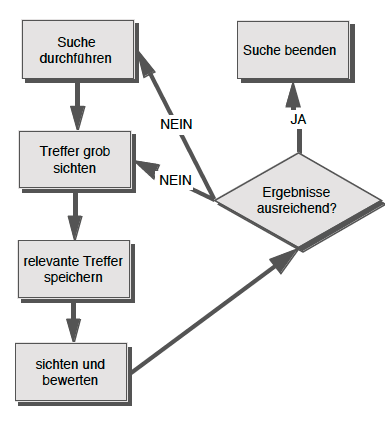
\includegraphics{images/recherchieren-internet-zyklischer-suchprozess-min} 

}

\caption{Der zyklische Suchprozess}\label{fig:unnamed-chunk-13}
\end{figure}

Betrachten Sie die Suche im WWW als zyklischen Prozess: nach der Suche
und Sicherung einer überschaubaren Anzahl von Ergebnissen folgt eine
Phase der Sichtung und Bewertung. Erst wenn diese abgeschlossen ist,
können Sie den weiteren „Materialbedarf`` feststellen und gezielt erneut
suchen oder die bereits erzielten Ergebnisse auf weitere Hinweise und
Hyperlinks prüfen.

Die Fragen, die Sie bei der Relevanzprüfung an eine Website stellen,
sind ganz ähnlich den Fragen bei der Relevanzprüfung von Büchern und
Artikeln (siehe Kapitel XXX „Recherchieren``). Um einen raschen
Überblick zu gewinnen, stehen Ihnen nun aber nicht die üblichen
Hilfsmittel wie Klappentext, Inhaltsverzeichnis oder Vorwort zur
Verfügung. In einem Hypertext gibt es andere Informationen und Hinweise:

\begin{itemize}
\tightlist
\item
  \emph{Adresse}: eine URL verrät meistens einiges über ihre Herkunft.
  Vor allem die „Top-Level-Domain``, also der letzte Teil des
  Domänennamens (= jener Teil der Adresse, der meist mit „www`` beginnt)
  ist genormt und gibt einen Hinweis auf Ursprung und Zielsetzung der
  Website (s. Aktionstabelle). Außerdem sind z. B. Universitäten
  meistens an ihren Domain-Namen erkennbar, in Deutschland beginnen sie
  sogar einheitlich mit „uni-\ldots{}``.
\item
  \emph{Startseite}: Die von der Suchmaschine gefundene Seite muss nicht
  die Startseite (home page) der Website sein. Suchen Sie die
  übergeordneten Seiten (über die in der Website (nicht im Browser)
  verfügbaren Schaltfläche „Home`` oder „Start``, über ein Menü, oder
  durch schrittweises Weglöschen der letzten Angaben bei der
  Web-Adresse). Da Websites sehr stark hierarchisch gegliedert sein
  können, ist die über die Schaltfläche „Home`` erreichbare
  Startseite/Homepage oftmals zu weit oben und zu allgemein für Ihre
  Zwecke, z. B. kann dieser Link direkt zur Eingangsseite des Instituts
  oder gar der Universität führen. Wichtig für die Relevanzprüfung ist
  die Startseite zum Thema, zur Person, zum Text.
\item
  \emph{Index oder site map}: Auf der passenden Startseite finden Sie
  meistens eine Art Inhaltsverzeichnis oder eine grafisch aufbereitete
  Übersicht über die Website (site map). Hier können Sie sich ein erstes
  Bild davon machen, was alles geboten wird. Allerdings ist diese
  Übersicht leider oft weniger aussagekräftig und zuverlässig als das
  Inhaltsverzeichnis eines Buches. Verweise können ins Leere gehen, und
  versprochene Inhalte fehlen oder sind dürftiger als angekündigt: da
  hinter einer Website kein prüfender Verlag steht, gibt es keine
  Garantie dafür, dass eine Website auch enthält, was ihr
  Inhaltsverzeichnis verspricht (siehe XXX „Webseiten auf Qualität
  prüfen``).
\item
  \emph{Breite untersuchen}: Rufen Sie daher (zumindest
  stichprobenartig) die einzelnen Punkte des Inhaltsverzeichnisses auf,
  um einen Überblick über Breite und Tiefe der Website zu erhalten. Sie
  können dabei auch einzelne Seiten „Probelesen``, wie Sie das beim
  Durchblättern eines Buches tun würden.
\item
  \emph{Tiefe untersuchen}: Finden Sie heraus, in welchem Kontext die
  gefundene Website steht. Sie gelangen so z. B. über die Liste der
  Publikationen der Autorin zu Angaben über die Person und weiter zur
  Institution oder Firma, in der die Autorin tätig ist. Sie können
  dadurch die Inhalte besser ein- und zuordnen.
\item
  \emph{Seitenzweige}: Möglicherweise finden Sie dadurch andere
  Publikationen und/oder Themen, die für Sie ebenfalls oder noch mehr
  von Interesse sind. Begnügen Sie sich in dieser Phase jedoch damit,
  diese Seiten für eine spätere Sichtung vorzumerken, also nur den Link
  abzuspeichern -- s. oben, „Zyklische Vorgangsweise``. Aufgrund dieses
  Suchlaufs in verschiedene Richtungen können Sie entscheiden:
\item
  \emph{Die Website ist nicht relevant} für Ihre Arbeit. In diesem Fall
  sollten Sie den gespeicherten Hyperlink löschen, um nicht später
  nochmals auf diese für Sie unbrauchbare Website „hereinzufallen`` und
  damit Zeit zu verschwenden.
\item
  \emph{Die Website ist relevant}. Wenn Ihr Browser es zulässt, sollten
  Sie zur gespeicherten Adresse einen kurzen Kommentar hinzufügen, der
  Inhalt und Bedeutung (für Ihre Arbeit) kurz zusammenfasst. Das ist als
  Erinnerungsstütze notwendig, denn nach der Sichtung von möglicherweise
  Dutzenden von Webseiten werden Sie garantiert nicht mehr Struktur und
  Inhalt jeder einzelnen Seite im Gedächtnis behalten haben. Webseiten
  auf Qualität prüfen Die oben beschriebene Methode der Sichtung einer
  Website gibt bereits gewisse Aufschlüsse über die Qualität Ihres
  Fundstücks: institutionelle Einbettung und Trägerschaft, „gepflegte``
  Webseiten, Umfang usw. Darüber hinaus beachten Sie auch noch:
\item
  \emph{Aktualität}: Webseiten sollten (meist am Ende) einen Vermerk
  tragen, wann sie zuletzt aktualisiert wurden. Ein weit zurückliegendes
  Datum kann bedeuten, dass die von der Seite weiterführenden Hyperlinks
  zu einem wesentlichen Teil veraltet sind. Dadurch kann die Website
  unbrauchbar sein für Ihre Zwecke -- muss aber nicht. Wenn es sich z.
  B. um einen Text (Skriptum, Buch \ldots{}) handelt, der eher in sich
  geschlossen ist, so kann er seine Gültigkeit durchaus über mehrere
  Jahre bewahren. Ob der Inhalt hingegen schon überholt und deshalb für
  Sie unbrauchbar ist, ist eine andere Frage, die Sie wie bei einem Buch
  selbst zu beurteilen haben.
\item
  \emph{Autorin}: Selbstdarstellung der Autorin sowie das
  Werkverzeichnis geben (falls vorhanden) Aufschluss über bisherige
  Tätigkeiten und Veröffentlichungen. Das liefert Hinweise wie: Hat die
  Autorin in angesehenen (peer-reviewed) Zeitschriften bzw. Verlagen zu
  diesem Thema veröffentlicht? Wie lange und wie intensiv ist die
  Autorin auf diesem Gebiet bereits tätig? Mit wem arbeitet die Autorin
  zusammen?
\item
  \emph{Institution}: Es versteht sich fast von selbst, dass die private
  Homepage eines Studenten mit mehr Vorsicht zu betrachten ist als
  Webseiten, die auf dem „offiziellen`` Server einer
  Forschungseinrichtung zu finden sind. (Die Einschränkung auf
  „offiziell`` ist notwendig, da oft Einzelpersonen auf einem
  Institutsserver ihre eigenen, mehr oder weniger privaten Webseiten
  präsentieren. Die Institution sollte zwar die Qualität und „political
  correctness`` aller Inhalte prüfen, die unter ihrem Namen im Web
  veröffentlicht werden, ist aber manchmal damit überfordert). Beim
  Server einer Forschungseinrichtung kann angenommen werden, dass die
  Inhalte bereits intern auf ihre Qualität geprüft wurden, denn
  inzwischen haben die meisten Institutionen begriffen, dass ihre
  Website dem Image ebenso schaden wie nutzen kann.
\item
  \emph{Wissenschaftlichkeit}: Bei der Betrachtung der Inhalte selbst
  ist zu prüfen, ob sie den formalen und inhaltlichen Ansprüchen an
  wissenschaftliche Arbeiten entsprechen. Zwar sind nicht alle Texte auf
  einem Webserver auch wissenschaftliche Texte und müssen es auch nicht
  sein. Eine informative, vielleicht sogar unterhaltsame Kurzdarstellung
  eines Instituts oder eines Forschungsprojekts erfüllt eher die Rolle
  einer (Werbe)Broschüre oder eines Ratgebers. Argumentatives Schreiben
  und Quellennachweise wären dem Zweck dieser Texte hinderlich. Was
  jedoch auch hier nicht fehlen darf, ist der Hinweis auf jene Stellen
  und Veröffentlichungen, in denen sich die Forschung und Argumentation,
  die zu den plakativen Aussagen oder praktischen Anleitungen geführt
  hat, nachvollziehen lässt. Sofern es sich bei den Webseiten um
  Online-Versionen von wissenschaftlichen Artikeln oder Bücher handelt,
  versteht es sich von selbst, dass die formalen (z. B.
  Quellennachweise) und inhaltlichen (z. B. Sachlichkeit, Logik,
  Nachvollziehbarkeit) Kriterien genauso erfüllt werden müssen wie in
  gedruckten Werken.
\end{itemize}

Auch hier sollten Sie streng sein bei der Auswahl und alle Web-Adressen,
die den Qualitätskriterien nicht genügen, aus Ihrem Verzeichnis wieder
entfernen.

\section{Material beschaffen}\label{material-beschaffen}

\subsection{Herunterladen und Drucken}\label{herunterladen-und-drucken}

Müssen Sie sich Materialien aus dem Internet erst noch „beschaffen``,
wenn Sie sowieso über Ihre gespeicherten Adressen darauf Zugriff haben?
Die Antwort auf diese Frage hängt von Ihren Arbeits- und
Lesegewohnheiten ab:

\begin{itemize}
\tightlist
\item
  Wenn Sie lieber Gedrucktes als Bildschirme lesen,
\item
  wenn Sie oft in den Materialien blättern und schmökern,
\item
  wenn Sie auch dort arbeiten wollen, wo Sie keinen PC oder
  Internet-Zugang haben,
\end{itemize}

dann werden Sie wahrscheinlich nicht darum herumkommen, die gefundenen
Webseiten auszudrucken und abzulegen. Häufig werden Artikel und längere
Texte im WWW nicht als Webseiten (in HTML) und zur Darstellung am
Bildschirm aufbereitet, sondern als Dokumente zum Herunterladen zur
Verfügung gestellt. Das am häufigsten dafür verwendete Dateiformat ist
PDF (portable document format).

PDF-Dateien können unabhängig vom Anwendungsprogramm, mit dem der Text
erstellt und formatiert wurde, am Bildschirm so dargestellt werden, wie
sie auch auf dem Papier erscheinen würden. Der Leser benötigt dazu nur
ein kostenloses Programm, den „Acrobat Reader``. PDF-Dateien können am
PC des Lesers nur dargestellt und (meistens) gedruckt, nicht aber als
Text bearbeitet oder kopiert werden. Das bringt für die AutorInnen den
Vorteil eines -- wenn auch geringen -- Schutzes vor Plagiaten.

Materialien aus dem Internet werden genau wie gedruckte Quellen in der
Literaturdatenbank oder -kartei erfasst. Dabei werden alle Angaben
gemacht, die später auch für das Zitieren von Quellen aus dem WWW
notwendig sind (siehe Kapitel „Zitieren``). Notieren Sie auf jeden Fall
die Web-Adresse (URL) sowie das Datum, an dem Sie das Material gesehen
bzw. heruntergeladen haben: diese werden bei Quellen aus dem Web
mitzitiert.

\subsection{Kauf im Internet}\label{kauf-im-internet}

Der Buchhandel hat als eine der ersten Sparten den Weg zum E-Commerce
genommen. Sie können praktisch alle deutschen und fremdsprachigen Bücher
über das Internet beziehen. Bezahlt wird dabei vorwiegend mit
Kreditkarte. Beim Bücherkauf im Internet ist zu beachten:

\begin{itemize}
\tightlist
\item
  \emph{Datensicherheit}: Kaufen Sie per Nachnahme oder mit der
  Kreditkarte. Kreditkarten-Daten sollten unbedingt in verschlüsselter
  Form übertragen werden. Der Web-Browser weist Sie durch eine Nachricht
  und/oder ein Symbol darauf hin, wann Sie eine „sichere`` Webseite
  aufrufen bzw. wieder verlassen. Bei Ihren Kundendaten und in e-Mails
  (Rechnung, Bestellbestätigung sollte höchstens ein Teil Ihrer
  Kreditkartennummer erscheinen, nie die ganze.
\item
  \emph{Verfügbarkeit und Lieferfristen}: Worauf bezieht sich die
  angegebne Lieferzeit? Es kann sich um die Zeit bis zur Auslieferung
  oder aber um die (ungefähre) Zeit bis zur Zustellung handeln. Im
  ersten Fall müssen Sie den Postweg noch dazurechnen.
\item
  \emph{Zustellung}: mit der Post oder mit einem Paketdienst? Wenn Sie
  zu den üblichen Arbeitszeiten selten an der Lieferadresse zu finden
  sind, kann das Zusammentreffen mit dem Paketdienst mühsam werden.
\item
  \emph{Warenkorb und Abbruch-Möglichkeit}: Meistens werden die
  gewählten Artikel in einem „Warenkorb`` gesammelt. Erst nachdem Sie
  die Suche beendet haben, gehen Sie zur „Kasse``, d. h. der Kaufvorgang
  beginnt. Sie müssen dabei korrekt über Preis, Versandkosten und
  Bedingungen informiert werden, noch bevor Sie den Kaufvorgang
  endgültig abschließen. Bis zum letzten „Okay`` müssen Sie die
  Möglichkeit bekommen, Ihre Bestellung zu ändern oder rückgängig zu
  machen.
\item
  \emph{Bestellbestätigung und Versandinformation}: Sie werden per
  E-Mail über Ihre Bestellung und den Bearbeitungsstand Ihrer Lieferung
  informiert.
\item
  \emph{Korrekter Zahlungsverkehr}: Wenn Sie mit Kreditkarte zahlen,
  prüfen Sie unbedingt, ob die Abbuchung von Ihrem Kreditkartenkonto mit
  dem Rechnungsbetrag übereinstimmt, bzw. ob die Beträge für nicht
  lieferbare oder zurückgegebene Artikel umgehend wieder gutgeschrieben
  werden.
\item
  \emph{Verwendung Ihrer Adresse}: Oft findet sich am Ende von
  Bestellformularen klein und leicht zu übersehen eine -- schon
  angekreuzte! -- Option, mit der Sie der Verwendung Ihrer Adresse für
  Aussendungen, Informationen usw. zustimmen. Wenn Sie sich vor einer
  E-Mail-Flut von Werbeaussendungen schützen wollen, lesen Sie das
  Bestellformular bis zum Ende durch und löschen Sie diese Markierung.
\item
  \emph{Rückgaberecht}: Sie müssen die Möglichkeit haben, die Ware
  innerhalb der gesetzlich vorgegebenen Fristen ohne Angabe von Gründen
  zurücksenden zu können und vollen Ersatz dafür zu bekommen.
\end{itemize}

Auch Börsen für antiquarische und/oder vergriffene Bücher sind im
Internet zu finden, wo entweder Buchhändler oder Privatpersonen als
Anbieter auftreten. Das Internet ist dafür besonders vorteilhaft -- denn
wer kann weltweit von Antiquariat zu Antiquariat pilgern, um ein
seltenes Buch zu finden?

Internet-Auktionshäuser haben sich in den letzten Jahren zu einem
gigantischen Marktplatz für gebrauchte, aber auch neue Produkte aller
Art entwickelt. Auch Bücher werden hier versteigert. Bevor Sie ein Buch
neu und teuer kaufen, können Sie also auch nachsehen, ob Sie es
ersteigern können. Beim Versteigern können Sie „Ihren`` Höchstpreis
eingeben, bis zu dem Sie automatisch mitsteigern. Beachten Sie dabei,
dass zum Preis noch die Versandkosten des Verkäufers dazukommen.
Außerdem müssen Sie die Zeit beachten: nach Auktionsende kommt der
Kontakt mit dem Verkäufer, Ihre Zahlung, und dann erst der (hoffentlich
prompte) Versand. Wenn Sie ein Buch sehr dringend benötigen, ist dieser
Weg also möglicherweise nicht geeignet.

Eine neue Entwicklung auf dem Sektor des elektronischen Buchhandels sind
„books on demand`` oder „e-books``: Dabei werden Bücher nicht mehr in
vorher festgelegten Auflagen gedruckt, sondern nur mehr auf Bestellung.
Das Buch bleibt digital gespeichert und kann daher nicht vergriffen
sein, Risiko und Kosten bleiben allerdings ausschließlich bei den
Autorinnen. Der Vertrieb erfolgt über einen eigenen Versand, aber auch
über den (Internet-)Buchhandel.

Beim elektronischen Kauf von einzelnen Artikeln müssen Sie ebenfalls auf
die Sicherheit achten. Viele Verlage und sonstigen Anbieter im Internet
bedienen sich für den Zahlungsverkehr wieder anderer Services (sozusagen
elektronischer Inkasso-Büros), bei denen Sie sich einmalig registrieren,
z.B. mit Ihrer Kreditkarte, und die den Zahlungsverkehr erledigen.

\section{Aufgabe: Recherchieren im
Internet}\label{aufgabe-recherchieren-im-internet}

\begin{longtable}[]{@{}l@{}}
\caption{\textbf{\label{tab:aufgabe3-test} Übungsaufgabe}}\tabularnewline
\toprule
\begin{minipage}[t]{0.97\columnwidth}\raggedright\strut
\begin{enumerate}
\def\labelenumi{\arabic{enumi}.}
\tightlist
\item
  Suchen Sie ein oder das Schlüsselwort zu Ihrem (eingegrenzten) Thema
  in der Wikipedia. Falls es zu Ihrem Suchbegriff keinen Eintrag gibt,
  probieren Sie ähnliche, v.a. übergeordnete Begriffe und gehen Sie den
  passenden Hyperlinks nach. \vspace{-6mm}
\end{enumerate}\strut
\end{minipage}\tabularnewline
\begin{minipage}[t]{0.97\columnwidth}\raggedright\strut
\begin{enumerate}
\def\labelenumi{\arabic{enumi}.}
\setcounter{enumi}{1}
\tightlist
\item
  Erweitern Sie die Literatursuche aus dem Kapitel „Recherchieren`` um
  die Recherche im Internet. Listen Sie mindestens 5 Websites (mit URL
  und Datum des Besuchs) auf, die für Ihr Thema relevant sind: Portale,
  Institutionen, Personen \ldots{} Kommentieren Sie die Websites kurz
  (Wer betreibt sie? Was findet man dort? Welche Bedeutung haben sie für
  Ihr Thema?)
\end{enumerate}\strut
\end{minipage}\tabularnewline
\bottomrule
\end{longtable}

\chapter{Kooperieren}\label{kooperieren}

\begin{figure}

{\centering 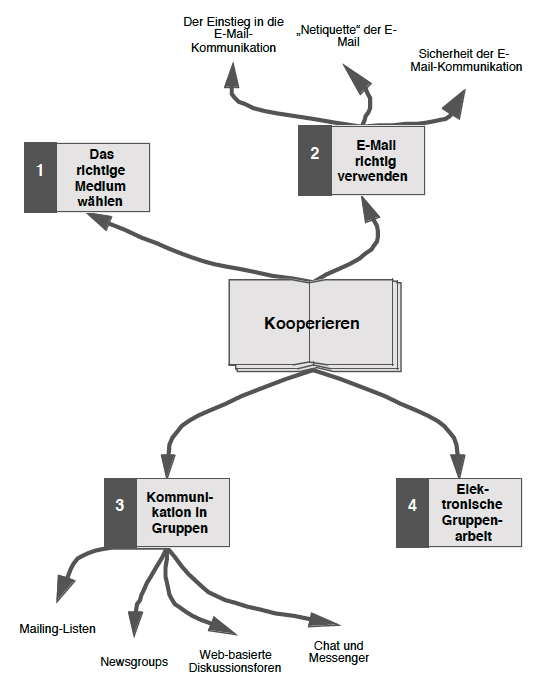
\includegraphics{images/kooperieren-min} 

}

\caption{Kooperieren (Überblick)}\label{fig:unnamed-chunk-14}
\end{figure}

Wissenschaft ist ein Diskurs: Erkenntnisse und Argumente werden
interpretiert, verglichen, kritisiert, und es werden daraus neue
Erkenntnisse gewonnen, die wieder als Argumente in den Diskurs
einfließen. Eine wissenschaftliche Arbeit ist ein Beitrag zu einer
fortlaufenden Diskussion, die im Fach oder zu einem seiner Teilgebiete
oder Spezialprobleme geführt wird. Während die Schritte und Regeln des
wissenschaftlichen Arbeitens dazu dienen, mit dem Beitrag „ordentlich``
an die vergangene Diskussion anzuschließen, ist das Vorstellen und
Veröffentlichen des Beitrags ein Angebot für die zukünftige Diskussion.
Durch die elektronische Kommunikation hat sich dieser Diskurs
beschleunigt: eigentlich kann es sich niemand mehr erlauben, jahrelang
für sich allein im stillen Kämmerlein zu lesen, zu grübeln und zu
schreiben. Außer bei Abschlussarbeiten -- die dadurch allmählich
unzeitgemäß werden -- ist Kooperation und Teamarbeit, auch über die
Grenzen von Ort, Zeit und Institutionen hinweg, gefragt. Kooperieren und
Kommunizieren wird damit zu einer wichtigen Fertigkeit im
wissenschaftlichen Arbeiten, die Sie bereits während des Studiums üben
und brauchen können.

Im Rahmen Ihrer wissenschaftlichen Arbeit werden Sie mit anderen
kooperieren und kommunizieren müssen, wenn Sie z.B.

\begin{itemize}
\tightlist
\item
  zusätzliche Informationen zu Ihrem Thema einholen wollen
\item
  graue Papiere, Forschungsberichte u. dgl. anfordern
\item
  mit einer Expertin zu Ihrem Thema ein persönliches Gespräch oder
  Interview anbahnen wollen
\item
  Ihre Arbeit oder Teile davon von Dritten durchlesen und kommentieren
  lassen möchten
\item
  Auskünfte über aktuelle, noch nicht veröffentlichte Forschungsarbeiten
  erhalten möchten.
\end{itemize}

Dieses Kapitel geht vor allem darauf ein, wie und mit welchen Techniken
kommuniziert und kooperiert wird: * Wie kontaktiert man
Wissenschafterinnen, an deren Arbeit und Meinung man interessiert ist? *
Wie benutzt man E-Mail richtig? * Wann und wie beteiligt man sich an
elektronischen Diskussionen? * Was ist Groupware und wofür wird sie
verwendet?

\section{Das richtige Medium wählen}\label{das-richtige-medium-wahlen}

Die Universitäten und Forschungsinstitute waren die Pioniere des
Internets. Nirgends wird daher die E-Mail schon so lang und so intensiv
genutzt wie zur Kommunikation in der Wissenschaft. Selbst die älteren
Jahrgänge unter den Professoren sind zum überwiegenden Teil ans Internet
angebunden und über E-Mail erreichbar. Es ist inzwischen durchaus
üblich, auch unbekannte Personen per E-Mail zu kontaktieren, wenn man
ihre Adresse z. B. als Kontaktadresse bei einer Veröffentlichung findet.
Wenn diese Adresse allerdings in einem Personenregister, etwa der
Universität, steht, gibt es keine Garantie dafür, dass diese Person die
E-Mail auch wirklich benutzt: die Adresse könnte automatisch vergeben
worden sein. Vielbeschäftigte lesen ihre E-Mail inzwischen oft nicht
mehr selbst, und manche lesen Nachrichten von unbekannten Absendern erst
gar nicht, weil sie automatisch oder manuell als „Spam`` kategorisiert
werden.

Neben dem neuen Medium der elektronischen Post gibt es die alten wie
Fax, Brief und Telefon auch weiterhin, und sie haben ihre Funktion nicht
verloren. Man muss also wissen, zu welchem Anlass und bei welchen
Partnern welches Medium das geeignete ist.

Faxgeräte sind zwar universal in ihrer Verbreitung, trotzdem ist es im
Wissenschaftsbetrieb nicht üblich, ohne andere vorhergehende Kontakte
einfach einen Brief zu faxen statt per Post zu schicken. Warum das so
ist, können wir beim besten Willen nicht sagen -- bei Firmen, va. wenn
es um Bestellungen und normale Geschäftsabwicklung geht, ist das gang
und gäbe.

Gefaxt werden im Wissenschaftsbetrieb in erster Linie: * Formulare wie
z. B. Anmeldungen zu Tagungen * dringende Texte, die noch vor der
„richtigen`` Sendung per Post ankommen sollen * Texte, Grafiken etc.,
die nicht in elektronischer Form vorliegen, aber schnell (und ohne
Rücksicht auf das Erscheinungsbild) übermittelt werden müssen. * Briefe
etc. nach vorheriger Abmachung bzw. Ankündigung

Außerdem wird das Fax natürlich auch zur raschen Übermittlung von Texten
an solche Personen verwendet, die keinen Zugang zum Internet haben oder
ihn nicht verwenden -- aber das werden immer weniger.

Die Briefpost spielt immer noch eine Rolle, aber ihre Funktion hat sich
geändert. Sie kommt jetzt dort zum Einsatz, wo ein „offizielles``
Dokument notwendig ist (Verträge, Rechnungen), bei formellen Anlässen
(Einladungen usw.) oder wenn Artikel, Unterlagen usw. mitgeschickt
werden. Schriftliches Material, das man den Empfänger zu lesen ersucht,
schickt man als Kopie, und zwar

\begin{itemize}
\tightlist
\item
  aus Höflichkeit, wenn man dem Empfänger das Dekodieren und Ausdrucken
  von elektronisch erhaltenen Dateien ersparen will.
\item
  aus Vorsicht: Der Adressat könnte die mitgeschickte Datei auch einfach
  ignorieren oder nicht nochmals anfordern, wenn sie nicht (richtig)
  angekommen ist.
\end{itemize}

Außerdem hilft der höhere Grad an Formalität eines Briefes in manchen
Fällen, etwas zu erreichen, weil es der Anfrage mehr Gewicht verleiht
und zeigt, dass der Sender sich Mühe gibt und auch „jemand ist``:
E-Mails sehen alle gleich aus, ein offizielles Briefpapier hingegen
repräsentiert etwas. Auf jeden Fall gibt man im Brief die eigene
E-Mail-Adresse an, wenn man eine hat: viele Adressaten werden dann
lieber gleich auf das weniger aufwendige, schnellere elektronische
Medium umsteigen.

Auch das Telefon wird durch die E-Mail nicht ganz und nicht immer
ersetzt werden können. Die (fern)mündliche Kommunikation ist geeignet,
um einen ersten Kontakt herzustellen, um Termine zu vereinbaren oder um
Fragen im Dialog zu klären. Ein intensives Gespräch, wo es um das
Aushandeln von Fragen geht oder auch darum, „Stimmung`` zu machen, wird
nach wie vor besser telefonisch (oder eben persönlich) geführt.

\section{E-Mail richtig verwenden}\label{e-mail-richtig-verwenden}

\subsection{Der Einstieg in die
E-Mail-Kommunikation}\label{der-einstieg-in-die-e-mail-kommunikation}

Voraussetzung für die Nutzung von E-Mail ist ein „Account`` (Konto) mit
einer E-Mail-Adresse. Zumindest eine Adresse ist beim Erwerb des
privaten Internet-Zugangs inbegriffen. Auch die Universitäten vergeben
E-Mail-Accounts an Studierende. Da der Studenten-Account aufgelöst wird,
wenn Sie das Studium beendet haben, ist es überlegneswert, sich eine
dauerhafte E-Mail-Adresse zuzulegen. Das kann z. B. ein kostenloser
Account bei einem web-basierten Freemail-Anbieter sein. Da es für
E-Mail-Adressen keine offiziellen Verzeichnisse gibt wie z. B.
Telefonbücher, besteht die Gefahr, dass Ihnen durch einen Wechsel der
E-Mail-Adresse viele Kontakte verloren gehen. Daher sollten Sie gleich
von Anfang an auf Kontinuität Ihrer E-Mail-Adresse achten.

Auf dem PC, an dem Sie Ihre elektronische Post erledigen wollen,
brauchen Sie ein Mail-Programm, einen sogenannten „Mail-Client``. Wenn
Sie am eigenen PC arbeiten, können Sie diesen Client so einrichten
(konfigurieren), dass die Verbindung mit den richtigen Informationen
(Benutzername, Passwort, Server-Adresse \ldots{}) automatisch aufgebaut
wird. Mail-Clients haben zumindest folgende Funktionen:

\begin{itemize}
\tightlist
\item
  \emph{Nachrichten senden und empfangen}: automatisch in regelmäßigen
  Abständen, wenn die Verbindung zum Server permanent ist, oder nur beim
  Starten und Beenden des Programms (z. B. bei Verwendung eines Modems)
  bzw. auf Befehl
\item
  \emph{Nachrichten schreiben}: Für das Schreiben gibt es ein
  Editor-Fenster mit einem leeren Formular, in das Adresse, Betreff etc.
  eingetragen und der Text verfasst wird.
\item
  \emph{Anlagen (Attachments) hinzufügen}: Beliebige Dateien können an
  eine E-Mail angehängt werden. Die Dateien werden in einem
  Dialogfenster ausgewählt und im E-Mail-Editor als Text oder Symbol
  angezeigt.
\item
  \emph{Nachrichten beantworten (Reply) und weiterleiten (Forward)}: bei
  „Reply`` wird wahlweise die ursprüngliche Nachricht „zitiert`` (s.
  unten). Bei diesen Funktionen werden jeweils alle bekannten Daten vom
  Programm in das Editor-Fenster übernommen. Beim Weiterleiten muss nur
  noch der neue Empfänger angegeben werden.
\item
  \emph{Kopien (Cc: = carbon copy) und „unsichtbare`` Kopien (Bcc: =
  blind carbon copy)} einer Nachricht senden: bei Cc: sieht der
  Empfänger, wer eine Kopie erhält, bei Bcc: hingegen nicht. Sie können
  „Bcc:`` daher zum Beispiel dafür verwenden, um dritte Personen
  sozusagen „inoffiziell`` über einen elektronischen Schriftverkehr auf
  dem Laufenden zu halten.
\item
  \emph{Nachrichten in Ordnern oder Mailboxen ablegen}, sortieren und
  suchen: diese Funktionen werden wichtig, sobald sich die E-Mails
  häufen.
\item
  \emph{Definition von Filtern und/oder Regeln}: Nachrichten können nach
  bestimmten Kriterien (z. B. Absender, ein Begriff im Betreff usw.)
  automatisch bearbeitet , z. B. in einen Ordner verschoben oder sogar
  beantwortet werden.
\item
  \emph{E-Mail-Adressen speichern und verwalten (Adressbuch)}: Meist
  können die Adressen direkt aus dem Adressbuch in das Editorfenster
  übernommen werden, und Adressen werden automatisch vervollständigt,
  wenn Sie sie im Adressfeld des Nachrichteneditors zu schreiben
  beginnen. Das hilft, die häufigen und lästigen Tippfehler beim
  Schreiben von E-Mail-Adressen zu vermeiden. Für gleichbleibende
  Adressatengruppen (z. B. eine Arbeitsgruppe) können Verteiler angelegt
  werden. Die Adressen müssen dann nicht mehr einzeln eingegeben werden.
\end{itemize}

\subsection{„Netiquette`` der E-Mail}\label{netiquette-der-e-mail}

„Netiquette`` sind Regeln für das gute Benehmen in der elektronischen
Kommunikation. Elektronische Nachrichten werden meistens nicht lange
entworfen und geplant, sondern schnell und spontan im Texteditor des
E-Mail-Clients getippt und abgesandt. Sie geraten daher kürzer und
informeller als Briefe. So hat sich ein bestimmter, sparsamer
„E-Mail-Stil`` entwickelt, z. B. durch die Verwendung

\begin{itemize}
\tightlist
\item
  von „Smileys``: aus Satz- und anderen Zeichen zusammengesetzte
  Gesichter, die verschiedene Gesichtsausdrücke und damit die
  Einstellung des Senders zum Geschriebenen andeuten. Durch ein
  Augenzwinkern etwa kann ohne viel Umschreibungen und Formulierungen
  ausgedrückt werden, dass das vorher Geschriebene nicht ganz ernst zu
  nehmen sei.
\item
  von Abkürzungen, die aus dem Amerikanischen stammen und ganze Formeln
  kurz fassen, wie z. B. IMHO = „in my humble opinion``.
\end{itemize}

Daneben zeichnet sich der geübte E-Mail-Benutzer aber noch durch ein
paar weitere Merkmale aus:

Manche Mail-Clients ermöglichen es, E-Mails im HTML-Format (Hypertext
Markup Language, siehe Kapitel „Publizieren``) zu versenden. Damit kann
der Text attraktiver gestaltet werden als mit ASCII-Zeichen. Doch
Vorsicht ist geboten: HTML-Mails sollten Sie nur an jemanden versenden,
von dem Sie wissen, dass sein E-Mail-Client ebenfalls HTML darstellen
kann. In allen anderen Fällen verzichten Sie besser darauf, um der
Empfängerin nicht das Lesen -- und Leben -- unnötig zu erschweren.

Selbst mit den eingeschränkten Mitteln des ASCII-Codes lassen sich
E-Mails übersichtlich und gut lesbar gestalten: Absätze, Leerzeilen und
Hervorhebungen (*, - o. ä.) reichen aus, um dem Empfänger einen guten,
schnellen Überblick zu gewähren.

Die „Betreff``-Zeile im Nachrichtenformular dient dazu, der Nachricht
einen Titel zu geben, der dem Empfänger gleich einen Hinweis auf den
Inhalt gibt. Ein aussagekräftiges „Subject`` anzugeben ist daher eine
wichtige Hilfe für den Empfänger. Wenn z. B. in einem Institut, einem
Projekt oder einer Arbeitsgruppe sehr viele Mails zu unterschiedlichen
Themen ausgetauscht werden, ist es sinnvoll, dem Betreff eine
Kurzbezeichnung des Bereichs oder Themas voranzustellen, zu dem die
E-Mail gehört. Das ist nicht nur eine wichtige Information für die
Empfängerin, sondern ermöglicht es ihr evt. auch, einen automatischen
Filter zu setzen, der die thematisch zusammengehörigen Mails in einem
Ordner sammelt. So kann z. B. vereinbart werden, dass alle E-Mails, die
das Projekt mit dem Akronym „GRZ`` betreffen, ein Subject der Art „GRZ:
Bericht``, „GRZ: Meeting``, „GRZ: Termin`` usw. erhalten sollen. Bei
großen Projekten mit vielen Beteiligten und Unterthemen kann dieses
System auch noch verfeinert werden. Das ist aber nur so lange sinnvoll,
als die Beteiligten nicht lange nachdenken müssen, in welchen
Unterbereich die Mail gehört, die sie gerade schreiben wollen -- dann
funktioniert das System nämlich nicht mehr.

Grundsätzlich sollte E-Mail rasch beantwortet werden. „Rasch`` kann
dabei alles zwischen fünf Minuten und drei Tagen bedeuten. Die E-Mail
hat die Korrespondenz enorm beschleunigt, und die Sender rechnen damit,
dass Sie die Nachricht praktisch unverzüglich beantworten. Bei den
zahlreichen E-Mail-Kontakten, die sich innerhalb kurzer Zeit bilden,
wurde das Abarbeiten der elektronischen Post daher inzwischen zu einer
zeitaufwändigen und oft störenden Dauerbelastung.

Bei zunehmendem E-Mail-Verkehr sollten Sie daher Ihren Umgang mit diesem
Medium organisieren und in vernünftigen Grenzen halten:

\begin{itemize}
\tightlist
\item
  Man kann E-Mail-Korrespondenz auch einmal ruhen lassen, wenn es nichts
  Relevantes zu sagen gibt, wenn z. B. ein Termin, eine gemeinsame
  Arbeit oder was immer erfolgreich vereinbart wurden.
\item
  Durch Anfragen, Aufforderungen usw., die eine gewisse Zeit zur
  Bearbeitung brauchen, sollten Sie sich nicht aus Ihrer Zeitplanung
  werfen lassen. Sie müssen das Geforderte nicht sofort beschaffen und
  senden, es genügt auch, eine kurze Antwort zu geben, in der Sie einen
  Termin nennen, zu dem Sie die Aufgabe erledigen können.
\item
  Planen Sie feste Zeiten für die Bearbeitung der E-Mail ein. Zwischen
  diesen Zeiten (zweimal täglich ist genug, außer in besonderen
  Situationen, wo rasche Reaktionen nötig sind) sollten Sie gar nicht
  nachsehen, was in Ihrer Mailbox eingelangt ist.
\end{itemize}

E-Mail-Systeme haben eine Reply- (Antwort-)Funktion, mit der man auf
eine erhaltene Nachricht reagieren kann, ohne nochmals Empfänger und
Titel angeben zu müssen. Dem Titel wird dabei ein „Re:`` oder „AW:`` (je
nach Programm) vorangestellt, sodass der Empfänger sofort sieht, welche
Nachricht hier beantwortet wird. Es ist eine schlechte (aber
verbreitete) Gewohnheit, eine eigentlich ganz neue Nachricht mit
„Reply`` zu schicken (um sich das Eintippen der Adresse zu ersparen),
aber den Betreff nicht neu zu vergeben.

Eine noch unangenehmere Unsitte ist es, die automatische
„quote``-Funktion unnötig zu verwenden. Bei dieser Funktion wird die
Antwort-Nachricht gleich so generiert, dass die ursprüngliche Nachricht
als Zitat wieder erscheint (mit \textgreater{} oder einem Strich am
Zeilenanfang markiert). Dieser Text ist editierbar, d. h. die Senderin
kann ihre Antworten, Kommentare usw. direkt in den ursprünglichen Text
einfügen. Alle für die Antwort nicht direkt relevanten Passagen sollen
weggelöscht werden.

Viele E-Mail-Benutzerinnen machen sich jedoch nicht die Mühe, den
überflüssigen zitierten Text wegzuschneiden, sondern schicken ihn
einfach wieder zurück -- oft mit nur ein paar Zeilen eigener Antwort
dazu. Der Empfänger muss dann mühsam in der zitierten (eigenen!)
Nachricht die wenigen neuen Schnipsel suchen. Besonders ärgerlich ist es
natürlich, einen Text von, sagen wir, drei Seiten samt und sonders
wieder zurückzubekommen, mit nicht mehr als einem angefügten „ok`` am
Ende.

In der E-Mail-Kommunikation hat sich ein Stil durchgesetzt, der der
nahen Verwandtschaft dieses Mediums mit dem mündlichen Austausch
Rechnung trägt. Es werden nicht viele Formalitäten gebraucht, ein
lockerer, hin und wieder sogar umgangssprachlicher Ton ist üblich,
selbst Tippfehler, die beim spontanen Schreiben schon mal vorkommen
können, werden toleriert. Trotzdem ist ein wenig Disziplin und
Aufmerksamkeit empfehlenswert. Treiben Sie z. B. die Spontaneität nicht
so weit, dass Sie jeden Gedanken, der Ihnen durch den Kopf geht, sofort
als E-Mail loslassen - vielleicht gleich ein paarmal hinereinander. Der
Empfänger wird mit dieser Menge an Botschaften keine Freude haben und
bald die Übersicht (und die Lust aufs Antworten) verlieren. Überlegen
Sie sich den Inhalt vor dem Schreiben, sammeln Sie ein paar Punkte in
einer einzigen Mail, und schreiben Sie klar und strukturiert.

Wenn man aber E-Mail wirklich als Ersatz für den traditionellen
Geschäftsbrief verwendet -- also z. B. für formelle Anfragen, für den
Erstkontakt mit unbekannten Personen -- ist es besser, auch die Sprache
danach zu richten und sich um Korrektheit in Ausdruck und
Rechtschreibung zu bemühen. Man zeigt damit Respekt, aber auch, dass
einem die Sache wichtig ist. In solchen Fällen sollte man auch auf die
speziellen E-Mail-Gebräuche wie Smileys und Insider-Abkürzungen
verzichten. Sie könnten despektierlich wirken, und außerdem weiß man
nicht im voraus, ob der Empfänger ein ebenso geübter E-Mail-Benutzer ist
und sie überhaupt versteht.

Die meisten E-Mail-Clients bieten die Möglichkeit, an jede Nachricht
automatisch eine „Signature`` -- eigentlich den Absender -- anzuhängen,
die der Benutzer selbst gestaltet. Zwar ist die E- Mail-Adresse des
Senders einer Nachricht dem Empfänger immer bekannt, aber erst die
Unterschrift enthält z. B. den vollen Namen, Postanschrift,
Telefonnummer und, immer öfter, auch die URL (WWW-Adresse) des Absenders
oder seiner Institution. Diese an die Nachricht angehängte Visitenkarte
sollte daher eigentlich in geschäftlichen E-Mails nie fehlen (unter
Freunden und Kollegen, die im dauernden engen Mail-Kontakt stehen, ist
sie nicht notwendig, sondern würde die E-Mails nur unnötig verlängern).
Ob man sie noch zusätzlich grafisch oder literarisch ausschmückt, bleibt
jedem selbst überlassen, sofern es nicht Richtlinien der eigenen
Institution (z. B. ein in ASCII-Zeichen gestaltetes Firmenlogo) zu
berücksichtigen gilt. Die meisten E-Mail-Clients erlauben es, zwischen
verschiedenen Signatures zu wählen, sodass Sie z. B. eine private und
eine geschäftliche oder eine deutsche und eine englische definieren und
je nach Bedarf verwenden können.

Die Sprache des Internet ist Englisch (eigentlich Amerikanisch), und
damit sind auch viele Gebräuche aus der nordamerikanischen
(Wissenschafts-)Kultur zu uns gekommen. Einer davon ist die formlose
Anrede mit Vornamen, die ja in einer Sprache, die keine Höflichkeitsform
kennt, ganz leicht und ohne großes Zeremoniell eingeführt werden kann.
Mit dem Nachnamen fallen dann auch gleich alle Titel unter den Tisch.

Solange man auf Englisch international kommuniziert, ist es auch ganz
leicht und angenehm, dabei mitzumachen. Wir Deutschsprachigen haben
allerdings anfangs Hemmungen, gleich selbst mit der Vornamen-Anrede und
dem formlosen Umgang anzufangen. Wenn Sie unsicher sind, wie Sie den
Partner anreden sollen, können Sie die erste E-Mail eher formell halten.
Geben Sie in der Unterschrift Ihren Vornamen an und warten Sie darauf,
ob der Empfänger in der Antwort gleich auf den Vornamen „umsteigt``. Sie
können dann sicher sein, dass Sie auch den Vornamen verwenden dürfen.

In der Kommunikation unter Deutschsprachigen setzen sich das Du und die
Vornamen zwar auch allmählich durch, aber noch ist es nicht üblich,
gleich von vornherein und automatisch damit anzufangen -- außer unter
Studierenden natürlich. In Zweifelsfällen muss man also beim Sie
bleiben, meist bis zum persönlichen Kennenlernen. Mit den Titeln
hingegen wurde und wird -- endlich -- kräftig aufgeräumt. In der E-Mail
(außer es handelt sich um einen „elektronischen Brief``, s. oben) nehmen
sich lange Titelwürste eher deplatziert und lächerlich aus.

\begin{longtable}[]{@{}l@{}}
\caption{\textbf{\label{tab:email} E-Mail richtig verwenden}}\tabularnewline
\toprule
\begin{minipage}[t]{0.97\columnwidth}\raggedright\strut
\begin{itemize}
\tightlist
\item
  Ist der „Betreff`` vorhanden, kurz und prägnant? Bezieht er sich genau
  auf den (wichtigsten) Inhalt der E-Mail?\vspace{-6mm}
\end{itemize}\strut
\end{minipage}\tabularnewline
\begin{minipage}[t]{0.97\columnwidth}\raggedright\strut
\begin{itemize}
\tightlist
\item
  Wird in der Antwort-Mail vom Ursprungstext nur so viel zitiert, wie
  für das Verständnis der Antwort notwendig ist? \vspace{-6mm}
\end{itemize}\strut
\end{minipage}\tabularnewline
\begin{minipage}[t]{0.97\columnwidth}\raggedright\strut
\begin{itemize}
\tightlist
\item
  Ist die E-Mail frei von Umlauten und Sonderzeichen?\vspace{-6mm}
\end{itemize}\strut
\end{minipage}\tabularnewline
\begin{minipage}[t]{0.97\columnwidth}\raggedright\strut
\begin{itemize}
\tightlist
\item
  Haben die Attachments ein Format, das der Empfänger mit größter
  Wahrscheinlichkeit lesen kann? \vspace{-6mm}
\end{itemize}\strut
\end{minipage}\tabularnewline
\begin{minipage}[t]{0.97\columnwidth}\raggedright\strut
\begin{itemize}
\tightlist
\item
  Werden die Attachments mit Inhalt und Format in der Mail angekündigt?
  Sind sie auch wirklich „beigelegt`` worden? \vspace{-6mm}
\end{itemize}\strut
\end{minipage}\tabularnewline
\begin{minipage}[t]{0.97\columnwidth}\raggedright\strut
\begin{itemize}
\tightlist
\item
  Sind Stil, Sprache und Schreibweise dem Zweck und Adressaten der E-
  Mail angemessen (weder zu förmlich noch zu vertraulich)? \vspace{-6mm}
\end{itemize}\strut
\end{minipage}\tabularnewline
\begin{minipage}[t]{0.97\columnwidth}\raggedright\strut
\begin{itemize}
\tightlist
\item
  Wird der Mail eine „Signature`` angehängt, und enthält diese alle
  wichtigen und aktuellen Kontaktinformationen? \vspace{-6mm}
\end{itemize}\strut
\end{minipage}\tabularnewline
\begin{minipage}[t]{0.97\columnwidth}\raggedright\strut
\begin{itemize}
\tightlist
\item
  Kommt in der Nachricht klar und strukturiert zum Ausdruck, was ich
  sagen möchte? \vspace{-6mm}
\end{itemize}\strut
\end{minipage}\tabularnewline
\begin{minipage}[t]{0.97\columnwidth}\raggedright\strut
\begin{itemize}
\tightlist
\item
  Ist der Text übersichtlich gegliedert und gestaltet?
\end{itemize}\strut
\end{minipage}\tabularnewline
\bottomrule
\end{longtable}

\section{Sicherheit der
E-Mail-Kommunikation}\label{sicherheit-der-e-mail-kommunikation}

Die größte Bedrohung aber, die von der Benutzung von E-Mail ausgeht,
stellen destruktive Inhalte dar, die mit Attachments verschickt werden.
Viren in E-Mails selbst sind zwar bei bestimmten Clients möglich, aber
viel seltener -- die Warnungen, die dazu hin und wieder verbreitet
werden, sind zum allergrößten Teil falsch, (also „Hoaxes``). Zur
Epidemie werden die bösartigen E-Mails, wenn sie in Form von „Würmern``
große Teile des Internets automatisch überschwemmen, indem sie z. B.
Adressverzeichnisse befallener Rechner benutzen. Attachments können auch
Computer-Viren enthalten, die den eigenen Rechner angreifen, wenn das
Attachment geöffnet wird.

Der automatische Schutz vor infizierten Attachments ist schwierig. Der
effektivste und einfachste Schutz aber ist, keine Attachments mit
unbekannten Dateien zu öffnen, insbesondere wenn Ihnen der Absender und
das Dateiformat fremd sind. Daher sollten auch Sie selbst nie an
Unbekannte unverlangt E-Mails mit Attachments ohne eine kurze
Vorankündigung versenden, z. B. im Rahmen von Blindbewerbungen.

Zusätzlich zu dieser Vorsichtsmaßnahme sollten Sie ein
Anti-Viren-Programm installieren. Diese Programme können allerdings nur
gegen Viren schützen, die bereits bekannt sind. Da immer wieder neue
Viren auftauchen, ist ein hundertprozentiger Schutz nicht möglich.
Unbedingt notwendig ist es, sich regelmäßig ein aktualisiertes Update
des Anti-Viren-Programms zu beschaffen.

Unter Umständen sollten Sie auch die Benutzung einer „Personal
Firewall`` in Betracht ziehen. Diese Programme schotten Ihren Rechner
vor Zugriffen von außen ab. Sehr sicher sind auch (Web- )Browser-Zugänge
zu Mailsystemen, wie sie von vielen Universitäten und kostenlosen
E-Mail-Diensten im WWW angeboten werden. Am besten hilft eine gesunde
Portion Misstrauen gegenüber „seltsamen`` E-Mails: kaum ein Virus kann
ohne die aktive Mitwirkung der Benutzer einen Schaden anrichten.

Benutzerinnen von E-Mail setzen im Geist oft fälschlicherweise E-Mails
mit Briefen gleich und vertrauen elektronischen Nachrichten alles an,
was sie gerne als Briefgeheimnis geschützt wissen wollen. Eigentlich ist
E-Mail aber besser mit offenen Postkarten zu vergleichen:
Mail-Administratoren und andere Personen, die sich Zugang zu Servern
verschaffen können, könnten zumindest theoretisch alles lesen, was da an
elektronischen Nachrichten eingeht. Auch die riesige Menge an E-Mails,
in denen die einzelne Nachricht wie die Nadel im Heuhaufen verschwindet,
ist nur ein theoretischer Schutz vor unbefugtem Lesen. Mit
Software-Unterstützung ist es auch kein Problem, Tausende von Mails nach
Schlüsselwörtern zu durchsuchen, was von staatlichen Geheimdiensten auch
gemacht wird.. Zwischen Firmen wurden bereits spektakuläre Fälle von
Betriebsspionage bekannt. In amerikanischen und britischen Firmen ist
das Abhören der E-Mails des Personals erlaubt und wird auch betrieben.

Die Verschlüsselung von E-Mails ist eine Möglichkeit, den Inhalt für
Unbefugte unleserlich zu machen. Sie wird allerdings nicht sehr häufig
verwendet -- offensichtlich fühlen sich die Benutzerinnen
(fälschlicherweise) sicher genug.

Das bekannteste Verfahren zur Verschlüsselung von E-Mails heißt Pretty
Good Privacy`` (PGP). Die Software dafür integriert sich transparent in
die meisten populären Mail-Clients und ermöglicht die sichere
Übertragung elektronischer Nachrichten. PGP benutzt einen öffentlichen
und einen privaten Schlüssel. Mit dem öffentlichen Schlüssel kann jede
beliebige Person eine Nachricht so verschlüsseln, dass nur die
Besitzerin des privaten Schlüssels diese wieder öffnen kann. Dieses
Verfahren ist vergleichbar mit einem sicheren Briefkasten, in den jeder
etwas hineinwerfen, aber nur der etwas herausnehmen kann, der den
privaten Schlüssel kennt.

PGP unterstützt außerdem digitale Signaturen zur Durchführung
rechtsgültiger Geschäfte im Internet, d. h. der Absender einer E-Mail
identifiziert sich eindeutig gegenüber einem Kommunikationspartner, der
dieser Nachricht daher vertrauen kann. Keine technischen Gegenmittel
helfen beim in letzter Zeit immer häufiger werdenen „Phishing`` (von
„Password Fishing``). Damit versuchen Betrüger, an persönliche Daten von
BenutzerInnen, vor allem natürlich an Kreditkartendaten und
E-Banking-Zugangsdaten, heranzukommen. Die Methode ist fast immer
gleich: Die Täter senden massenhaft Mails, die einen getarnten Link zu
einer Website enthalten, auf der man seine Daten eingeben soll. Der
Vorwand ist meist eine angebliche Sicherheitsüberprüfung, z.T. weil
vorgeblich Daten verloren gegangen oder missbraucht worden seien. Der
Link sieht in den HTML-Mails auf den ersten Blick aus, als führe er zur
Website des Unternehmens, von dem die Mails vorgeblich kommen. Teilweise
wird eine Grafik eingebunden, die wie Text aussieht, aber als Ganzes mit
einem Link zur Website der Betrüger versehen ist. Vorzugsweise werden
als Absender Banken und Kreditkartenunternehmen vorgetäuscht, aber auch
eBay wurde bereits benutzt. Hier hilft nur Misstrauen: seriöse
Unternehmen würden niemals auf diese Art Ihre Daten abfragen! Löschen
Sie eine derartige Mail schon beim geringsten Zweifel oder prüfen Sie
die Seriosität, z. B. in der Liste bereits bekannter
Phishing-Betreffzeilen beim Hoax-Service der TU Berlin (hoax.info.de).

Dieses Service sammelte ursprünglich, wie der Name sagt, „Hoaxes``, also
Falschmeldungen, ursprünglich über Computer-Viren. Die Empfänger werden
aufgefordert, die e-Mail an möglichst viele Adressen weiterzusenden.
Verwandt mit dieser Art der Internet-Verschmutzung sind elektronische
Kettenbriefe. Der Versuch, auf diese Weise Geld zu erschwindeln, ist
illegal („Pyramidensysteme``), aber es gibt offensichtlich genügend
E-Mail-Benutzer, die Glücksverheißungen, Spendenaufrufe oder Petitionen
(die oft schon jahrelang kursieren) naiv weiterleiten. Bevor Sie einen
solchen Aufruf weiterleiten, prüfen Sie immer, am besten beim
Hoax-Service, ob es sich um eine seriöse E-Mail handelt oder um einen
Hoax; Sie ersparen damit Ihren Freunden und Bekannten unnötige E-Mails.

Weniger eine Bedrohung der Sicherheit als eine Belästigung stellen die
„Spam-Mails`` und „Junk-Mails`` dar. „Spam`` hat sich als Bezeichnung
für unverlangte Werbung in E-Mails und Newsgruppen eingebürgert. Die
Erfinder und Urheber von Spams überschwemmen das Internet mit Millionen
von Nachrichten und bezahlen dafür quasi nichts, während die
Empfängerinnen die Mails auf eigene Kosten (zumindest an Zeit)
herunterladen und ansehen.

Während früher Versprechungen schnellen Gewinns überwogen („Make money
fast``, „Earn \$ 1000 a week`` usw.), sind es derzeit vor allem Angebote
an Pharmaka und Pronografie, sowie (ebenfalls ein Dauerbrenner) dubiose
Geldwasch-Angebote angeblicher Nachfahren angeblicher afrikanischer
Politiker.

Provider (ob privat oder universitär) verwenden inzwischen Spam-Filter,
die bereits serverseitig die einlangenden E-Mails sortieren und
gegebenenfalls als „Spam`` markieren. Alle gängigen E-Mail-Programme
besitzen Funktionen für das Filtern von Nachrichten, die beim Eintreffen
von E-Mails mit bestimmten, benutzerdefinierten Schlüsselwörtern im Text
aktiv werden. Damit können die von Provider-Seite erkannten Spams sofort
in einen eigenen Ordner aussortiert werden. Sie können diesen Ordner von
Zeit zu Zeit durchsehen, ob nicht doch eine seriöse Mail irrtümlich
ausgefiltert wurde, bevor Sie die hier gesammelten Mails löschen. Sie
können auch zusätzliche Filter definieren oder einen (zusätzlichen)
Spam-Filter client-seitig installieren.

Die E-Mail-Adressen für Spam-Mails werden automatisiert durch
Durchsuchen des WWW gewonnen. Eine wirkungsvolle Gegenmaßnahme ist
daher, Ihre E-Mail-Adresse im Web (Adressverzeichnisse, Webseiten usw.)
in einer Form zu veröffentlichen, die das maschinelle Lesen unmöglich
macht: z. B. nicht als Text, sondern als Bild, oder so, dass die
Benutzerinnen sie erst zusammen- oder übersetzen müssen, wie etwa
walter.mayer@, wobei an ganz anderer Stelle und nur als Domäne, z.B.
„bestefirma.com`` angegeben wird.

\section{Kommunikation in Gruppen: Foren, Newsgroups,
Listen}\label{kommunikation-in-gruppen-foren-newsgroups-listen}

E-Mails sind Fortsetzungen des Briefverkehrs und Telefonierens, da sie
sich auf die Kommunikation zwischen zwei Personen beschränken. Das
Internet ermöglicht jedoch auch die Kommunikation in Gruppen, wie sie -
außer etwa in den eher seltenen Telefonkonferenzen - ohne dieses Medium
kaum möglich waren und wären. Newsgroups, Diskussionsforen und
Mailing-Listen sind Mischungen aus Informations- und Diskussionsmedien.
Ob sie mehr dem einen oder dem anderen Zweck dienen, hängt vom Thema und
von den Teilnehmerinnen ab, kann sich aber auch sehr schnell ändern. Die
Unterschiede sind daher weniger inhaltlicher Art als in der Art der
Verbreitung und Benutzung.

\subsection{Mailing-Listen}\label{mailing-listen}

Mailing-Listen verwenden als Medium die E-Mail. Sie werden von
List-Servern verwaltet: das sind Programme, die mehrere (oft Tausende)
verschiedene Mailing-Listen mit ihren jeweiligen Teilnehmern bewältigen
und Nachrichten gezielt an die jeweilige Gruppe -- per E-Mail --
aussenden. Die gesamte Kommunikation in und mit einer Mailing-Liste wird
über E-Mail abgewickelt.

Auf Mailing-Listen zum Thema der eigenen Arbeit stößt man oft durch
Hinweise in Zeitschriften und vor allem auf Websites. Es gibt aber auch
spezielle Dienste im WWW, mit denen Sie gezielt nach Listen zu
bestimmten Themen suchen können.

Um an einer Mailing-Liste teilnehmen zu können, müssen Sie sich anmelden
bzw sie abonnieren („subscribe``). Die Schritte, die Sie vornehmen
müssen, um sich in eine Mailing-Liste einzuschreiben, werden mit der
Ankündigung oder Einladung zur Liste mitgegeben. Meist wird heute ein
Web-Formular für An- und Abmeldung angeboten. Eine Anweisung per E-Mail
könnte z. B. so aussehen:

\begin{quote}
To:
\href{mailto:mailbase@mailbase.ac.uk}{\nolinkurl{mailbase@mailbase.ac.uk}}
Subject: empty Body: subscribe
\end{quote}

Generell wird ein Mail-Server durch Befehle gesteuert, die der Benutzer
per E-Mail sendet. Sie müssen so geschrieben werden, dass der Server sie
„verstehen`` und automatisch verarbeiten kann. Dazu gehören:

\begin{itemize}
\tightlist
\item
  die E-Mail-Adresse des Servers (die nicht dieselbe ist wie die der
  Liste): z. B.
  \href{mailto:mailbase@mailbase.ac.uk}{\nolinkurl{mailbase@mailbase.ac.uk}}
  als Server-Adresse und
  \href{mailto:englit@mailbase.ac.uk}{\nolinkurl{englit@mailbase.ac.uk}}
  als Listenname.
\item
  eine leere Subject-Zeile (manche Server ignorieren diese Zeile aber
  sowieso)
\item
  der richtige, korrekt geschriebene Befehl (oder eine Befehlsfolge) im
  Text („body``) der Nachricht
\item
  ohne vor- und nachgestellten Text, d. h. die Signature kann
  Fehlermeldungen verursachen! Daher: in diesem Fall weglassen oder als
  letzte Befehlszeile vorher einen Abbruchbefehl (meist „stop``)
  schreiben: der Server verarbeitet dann die nachfolgenden Zeilen nicht
  mehr.
\end{itemize}

Mit dem Gegenbefehl „unsubscribe `` kann man die Zustellung von
Nachrichten wieder beenden. Manche Server erlauben oder verlangen, einen
Benutzernamen anzugeben. Sich per Namen vorzustellen, gehört zum guten
Ton in seriösen Listen. Deshalb wird man den Namen bei der Subskription
angeben, auch wenn es nicht unbedingt erforderlich ist.

List-Server bieten unterschiedlichen Komfort für ihre Benutzer. Zu den
weiteren Optionen kann gehören:

\begin{itemize}
\tightlist
\item
  „review `` (an den Mail-Server): sendet eine Liste der Teilnehmer.
  Diese Option kann für „normale`` Benutzer aber auch gesperrt sein.
\item
  Archiv: Zugriff auf frühere Beiträge aus der Mailing-Liste, meist
  chronologisch geordnet. Die Befehle dazu -- wenn verfügbar -- finden
  sich in der jeweiligen Gebrauchsanleitung.
\item
  Dateien: Textdateien können den Listenmitgliedern als Dokumente auf
  dem Server zur Verfügung gestellt werden, ohne dass sie als
  Listen-Aussendungen verbreitet werden.
\item
  Unterbrechung: („suspend`` o.ä.) Die Zusendung von Listenbeiträgen
  wird damit unterbrochen (z. B. während des Urlaubs), aber die
  Mitgliedschaft bleibt aufrecht.
\end{itemize}

Die für den jeweiligen Listserver geltenden Befehle können Sie über
E-Mail beziehen oder im WWW nachsehen. In den meisten Fällen erhalten
Sie nach dem Abonnieren der Liste eine automatisch generierte
Begrüßungsmail, in der Sie auch gleich Hinweise zur Benutzung bekommen.
Meistens werden heute Web-Formulare für die An- und Abmeldung sowie für
die Konfiguration verwendet.

Mailing-Listen haben immer zumindest einen „list owner`` (Eigentümer).
Das ist meistens der Gründer und (hoffentlich) auch eine Person, die
sich für Qualität und Inhalte verantwortlich fühlt. Der Eigentümer kann
bestimmte Eigenschaften der Liste definieren, z.B.

\begin{itemize}
\tightlist
\item
  offen oder geschlossen: in eine geschlossene Liste können nur durch
  die Eigentümer Mitglieder aufgenommen werden. Subskribieren durch die
  Benutzer selbst ist nicht möglich. Geschlossene Listen sind daher für
  Gruppen geeignet, die „unter sich`` bleiben und die Liste als internes
  Kommunikationsmittel verwenden wollen.
\item
  moderiert oder unmoderiert: Bei moderierten Listen gehen Beiträge von
  Teilnehmern nicht direkt an alle anderen Teilnehmer weiter, sondern
  zuerst durch die Mailbox des „Moderators``, der sie auswählen,
  verändern, ignorieren oder auch an individuelle E-Mail-Adressen statt
  an die Liste weitergeben kann. Der Vorteil ist, dass die in manchen
  großen Listen lästige Überschwemmung mit Beiträgen eingedämmt werden
  kann. Der Nachteil kann sein, wenn der Moderator eine Art Zensur
  ausübt -- was aber gegen die Netiquette ist. Leider sind gerade Listen
  mit vielen Beiträgen (z.~B. zu Software- oder Programmierfragen) meist
  nicht moderiert, weil niemand den großen Aufwand leisten will oder
  kann.
\end{itemize}

Neue Teilnehmer einer Liste beschränken sich am Anfang meistens darauf,
die eintreffenden Nachrichten zu lesen. Damit bekommen sie einen
Einblick in Inhalte, Interessen der Teilnehmer und den „Umgangston``
dieser speziellen Liste. Für viele Teilnehmerinnen ist das Lesen der
(oder einiger ausgewählter) Beiträge auch alles, was sie wollen: für sie
ist die Liste ein Informationsmedium, das sie über ein bestimmtes Thema
auf dem Laufenden halten soll. So können Sie z. B. bei der
Materialsammlung einschlägige Mailing-Listen abonnieren. Die Beiträge
selbst wie auch die (in guten Listen) häufigen Hinweise auf Literatur
und Websites können wertvolle Hinweise liefern.

Der nächste Schritt zur aktiven Teilnahme ist die Beantwortung einer in
der Liste gestellten Frage oder die Reaktion auf ein Problem, das gerade
diskutiert wird. Der Benutzer verwendet dazu die „Reply``-Funktion. Zur
Abfassung der Antwort gelten die selben Spielregeln wie für die E-Mail
im allgemeinen. Nur ist es in einer Antwort, die (bei einer
unmoderierten, „reply-to-list``-Liste) direkt wieder an sämtliche
Teilnehmer verbreitet wird, womöglich noch störender, wenn die Antwort
den gesamten Urprungstext nochmals zitiert (oder sogar, als Antwort auf
eine Antwort, den gesamten Urspungstext plus die gesamte erste Antwort).
Man sollte auch nur antworten, wenn man wirklich etwas zu sagen hat, und
nicht einfach Zustimmung oder Ablehnung kundtun: das interessiert die
übrigen Teilnehmer, die einen ja doch nicht kennen, herzlich wenig.

Ein wichtiger Grundsatz bei der Reaktion auf Mailing-Listen-Beiträge
ist: Eine Reaktion wird nur dann an die gesamte Liste ausgesendet, wenn
sie von allgemeinem Interesse ist. Wenn sie nur den Sender betrifft, so
adressiert man sie an ihn persönlich. Sollte z. B. ein Neuling in einer
Liste eine Verständnisfrage stellen, die für alle anderen Teilnehmer
längst geklärt ist, so wird sich (hoffentlich) ein Teilnehmer finden,
der ihm diese Frage in einer persönlichen E-Mail beantwortet, ohne mit
der Antwort das gesamte Listenpublikum zu langweilen.

Schließlich können Sie als Teilnehmerin daran interessiert sein, eigene
Gedanken der Liste zur Diskussion zu präsentieren. Auch wenn Sie sehr
viel zu sagen hätten: Der Umfang eines Beitrags sollte den eines
Thesenpapiers nicht übersteigen, und auch auf diese Art formuliert sein:
kurz, prägnant und auf die offenen Punkte hin ausgerichtet. Hier ist
nicht der Platz für ausführliche Argumentationen und Beweisführungen.
Sollten die Thesen oder Fragen Interesse und Anklang finden, werden die
anderen Teilnehmer schon von selbst genauer nachfragen oder evt. die
ganze Arbeit, auf der der Beitrag gründet, haben wollen. Der ideale
Beitrag sollte daher pointiert auf eine These oder Frage hinauslaufen,
die deutlich zur Diskussion gestellt wird. Um die Diskussion anzuregen,
kann der Sender sich bewusst bei der Darstellung seiner eigenen Position
dazu zurückhalten und diese erst später einbringen.

Wer sich eine seriöse Diskussion in einer Mailing-Liste wünscht, muss
dazu auch selbst beitragen. Dazu gehört, dass man bei eigenen Beiträgen
auch ein wenig über sich selbst sagt -- z. B. an welchem Thema man
arbeitet und in welchem Zusammenhang die gestellte Frage aufgetreten
ist. Anders ausgedrückt: es soll deutlich werden, dass der Sender
ernsthaft an einer Diskussion seines Beitrags interessiert ist. In
weiterer Folge kann das bedeuten, dass man für diese Diskussion -- falls
sie in Gang kommt -- ein wenig „Moderator`` spielen muss: d. h. die
eingelangten Reaktionen zusammenfassen und kommentieren und das
„Ergebnis`` wieder an die Liste zurückgeben.

Die zeitverzögerte Kommunikation zwischen Menschen unterschiedlichster
Herkunft und Muttersprache, die sich meist nicht persönlich kennen, ist
erfahrungsgemäß sehr anfällig für Missverständnisse, die dann leicht zu
ungezügeltem verbalem Schlagabtausch („Flaming``) führen können.
Überlegen Sie daher dreimal oder noch öfter, bevor Sie einen Beitrag,
den Sie abgrundtief falsch finden und der Sie aufregt, in scharfem Ton
beantworten! Gehen Sie zuerst einmal davon aus, dass der Autor sich
ungeschickt ausgedrückt hat oder dass Sie etwas missverstanden haben.
Formulieren Sie dann Ihre Kritik ganz vorsichtig, indem Sie immer die
Möglichkeit einräumen, dass Sie etwas nicht oder falsch verstanden
haben, und indem Sie dem Autor immer die Tür offenlassen, sich ohne
Gesichtsverlust zu korrigieren. Verstimmungen entstehen in der
elektronischen Kommunikation sehr leicht, sind aber umso schwerer wieder
auszuräumen.

\subsection{Newsgroups}\label{newsgroups}

Während Mailing-Listen mit Rundbriefen verglichen werden könnten,
erinnern Newsgroups vom Konzept her eher an öffentliche Anschlagtafeln:
wer nicht vor der Tafel stehenbleibt und selbst nachsieht, was es Neues
gibt, wird es nicht erfahren. Eine Newsgroup muss man daher „aktiv``
besuchen. Die dazu notwendige Software ist in den Internet-Browsern
integriert. Die Newsgroups werden von News-Servern verwaltet: der
Browser braucht daher die Adresse eines News-Servers, um die Information
von dort auf den Bildschirm des Benutzers zu holen.

Es gibt so viele Newsgroups -- von weltweit bis lokal, und das zu allen
nur erdenklichen (und noch mehr kuriosen) Themen -- dass kein Server sie
alle „führt``. Die Auswahl ist jedoch trotz dieser Filterung noch
überwältigend -- aber eben von Server zu Server ein wenig anders, v. a.
bei den regionalen Gruppen. Auch für Newsgroups gibt es Suchdienste im
Internet.

Die Namensgebung der (Usenet-)Newsgroups folgt einem hierarchischen
Schema, das die Suche ein wenig erleichtert. Die Namen beginnen mit
Hauptgruppen wie comp (Computer), misc (Miscellaneous), alt
(Alternative) u. a. Dazu kommen die regionalen Gruppen, die mit dem
Internet-Landeskürzel beginnen, also at, de, ch usw. Nach diesen
Hauptgruppen wird der Name in bis zu vier Stufen weiter spezifiziert, z.
B. misc.educ.lang.eng (eine Newsgroup zum Thema Englisch-Unterricht)
oder alt.pets.dogs.food (zum Thema Hundeernährung).

Man braucht dieses riesige Verzeichnis aller Newsgroups nicht jedesmal
zu durchsuchen, um die gewünschte zu finden: die Browser-Software
ermöglicht es, eine Auswahl zu treffen, die dann jedesmal beim Aufruf
erscheint und mit der man die gewünschte Gruppe aufrufen kann. Hier wird
auch gleich angezeigt, ob und wie viele neue Beiträge seit dem letzten
„Besuch`` eingelangt sind.

Will man einer Diskussion in einer Newsgroup wirklich folgen, so muss
man sich angewöhnen, sie regelmäßig aufzusuchen. Die News-Server halten
die Beiträge nämlich nur kurze Zeit gespeichert, danach gibt es sie
nicht mehr -- es gibt kein Archiv wie in manchen Mailing-Listen.

Die grafische Benutzeroberfläche der Internet-Browser macht das
Verfolgen einer Newsgroup-Diskussion bequem: Sie stellen die Beiträge in
einer hierarchischen Ordnung dar, aus der ersichtlich ist, welcher
Beitrag eine Antwort auf welchen anderen ist („threads``). Aus dem
Verzeichnis kann man die Artikel, die man lesen möchte, mit Mausklick
einfach auswählen. Die Beantwortung oder das Absenden eines eigenen
Beitrags sind genau so einfach.

Im Unterschied zu Mailing-Listen sind Newsgroups „öffentlich``
zugänglich: Jeder kann zu jedem Zeitpunkt jede Newsgroup aufsuchen. Das
heißt einerseits, dass das Publikum einer Newsgroup im Prinzip unbekannt
ist: man weiß nicht, wer einen Beitrag lesen wird. Andererseits ist eine
Newsgroup aber auch für alle Beiträge im Prinzip offen (allerdings gibt
es auch moderierte Newsgroups), und das bedeutet, dass eine unmoderierte
Newsgroup nicht gegen Nonsense, Beschimpfungen, Propaganda, Werbung,
Rassismus, Pornographie \ldots{} geschützt ist.

Immer wieder tauchen solche „Postings`` (= Beiträge) in den Newsgroups
auf, und nicht nur in einzelnen: Die Versender solcher Beiträge benutzen
Programme, die automatisch alle oder bestimmte Newsgroups aufsuchen und
den Beitrag dort deponieren. Zusätzlich werden Methoden verwendet, die
die Herkunft des Beitrags verschleiern. Diese „Spamming`` genannten
Aktionen sind für den Benutzer lästig bis ärgerlich; insgesamt
beeinträchtigen sie die Brauchbarkeit der Newsgroups als seriöses Medium
der Information und Diskussion -- Mailing-Listen haben in dieser
Beziehung einen etwas besseren Ruf, doch bei beiden Formen kann nur die
Moderation wirklich die Qualität sicherstellen.

In Newgroups und Web-Foren kommt manchmal ein rüder Umgangston auf.
Grund dafür sind oft „Flames`` genannte aggressive oder beleidigende
Beiträge, die dann Antworten auf dem selben Niveau hervorrufen. Solche
Entgleisungen können zu wüsten Beschimpfungen aller Teilnehmer
untereinander ausufern, die schließlich jede normale Diskussion
unmöglich machen und ein Forum lahmlegen. Für offene Diskussionsgruppen
gilt daher noch mehr als für Mailing-Listen, dass auf Mäßigung und
Zurückhaltung beim „Posten`` geachtet werden muss. „Flames`` sollten
einfach ignoriert werden -- jede Antwort schaukelt die fruchtlose
Streiterei nur auf.

Für Beiträge in Newsgroups gelten dieselben Spielregeln wie für
Mailing-Listen. Es ist allerdings nicht ratsam, die vollständige
„Signature`` anzuhängen: Newsgroups sind eben öffentlich, und man weiß
nicht, wem und für welche Zwecke man so seine Adresse in die Hände gibt.

\subsection{Web-basierte
Diskussionsforen}\label{web-basierte-diskussionsforen}

In den letzten Jahren haben sich web-basierte Diskussionsforen gegenüber
den Newsgroups durchgesetzt, da für sie kein spezielles Clientprogramm
benötigt wird. Sie können mit dem gewohnten Web-Browser benutzt werden.
Ein weiterer Vorteil ist, dass sie in eine Website eingebunden sind, die
Hintergrundinformation liefert und gleichzeitig auch als Archiv für die
Beiträge dienen kann.

Web-basierte Diskussionsforen findet man auch meistens über Websites,
die sich mit einem bestimmten Thema beschäftigen und dazu als
zusätzliches Service diese Austauschmöglichkeit für die Leserinnen
anbieten. Ob dieses Service auch angenommen wird und das Forum daher
„lebt``, ersieht man aus der Zahl der Beiträge und der Reaktionen darauf
und aus Datum und Absender der Beiträge: mehrere Beiträge pro Tag von
wechselnden Autorinnen sind ein Hinweis darauf, dass das Forum eine
ausreichend breite und interessierte Leserschaft erreicht.

In Bedienung und Umgangsformen unterscheiden sich web-basierte Foren
nicht von den Newsgroups. Beiträge werden über Web-Formulare eingegeben
und gesendet. Diskussionsforen im Web können geschlossen sein, d. h. Sie
brauchen eine Zugangsberechtigung (Benutzername und Passwort), um
teilnehmen zu können. Damit verbinden diese Foren den Komfort der
Newsgroups mit der „Privatsphäre`` der Mailing-Listen. Andere Foren sind
zwar für lesenden Zugriff offen, aber nur eingetragene Mitglieder können
schreiben. Achten Sie auf die Art des Forums, bevor Sie Persönliches
oder Dritte Betreffendes veröffentlichen.

\begin{longtable}[]{@{}l@{}}
\caption{\textbf{\label{tab:elektronische-diskussionen} An elektronischen
Diskussionen teilnehmen}}\tabularnewline
\toprule
\begin{minipage}[t]{0.97\columnwidth}\raggedright\strut
\begin{itemize}
\tightlist
\item
  Habe ich mich mit Inhalt und Ton der Gruppe vertraut gemacht, bevor
  ich selbst Beiträge schreibe? \vspace{-6mm}
\end{itemize}\strut
\end{minipage}\tabularnewline
\begin{minipage}[t]{0.97\columnwidth}\raggedright\strut
\begin{itemize}
\tightlist
\item
  Ist meine Antwort für die Gruppe von Interesse, oder sollte sie nur
  per E- Mail an den Absender gelangen? \vspace{-6mm}
\end{itemize}\strut
\end{minipage}\tabularnewline
\begin{minipage}[t]{0.97\columnwidth}\raggedright\strut
\begin{itemize}
\tightlist
\item
  Wird in der Antwort der zitierte (Ursprungs)Text auf das zum
  Verständnis Notwendige gekürzt? \vspace{-6mm}
\end{itemize}\strut
\end{minipage}\tabularnewline
\begin{minipage}[t]{0.97\columnwidth}\raggedright\strut
\begin{itemize}
\tightlist
\item
  Ist die Antwort/das Posting sachlich und höflich formuliert? (keine
  Kraftausdrücke, übertriebene Schärfe, persönliche Angriffe („flames``)
  \vspace{-6mm}
\end{itemize}\strut
\end{minipage}\tabularnewline
\begin{minipage}[t]{0.97\columnwidth}\raggedright\strut
\begin{itemize}
\tightlist
\item
  Gehe ich auf Fragen, Einwände usw. zu meinen eigenen Postings ein?
\end{itemize}\strut
\end{minipage}\tabularnewline
\bottomrule
\end{longtable}

\subsection{Chat, Messenger und
Internet-Telefonie}\label{chat-messenger-und-internet-telefonie}

Chats sind synchrone (zeitgleiche) elektronische Diskussionen. Alle
Beiträge werden (beinahe) sofort für alle Beteiligten sichtbar
dargestellt und können sofort beantwortet werden. Das „klassische``
Medium für Chats ist IRC (Internet Relay Chat). Es wird dafür ein
eigenes Client-Programm benötigt. Die meisten Chats sind heute aber ins
WWW eingebunden und benötigen keinen eigenen Client mehr.

„Chatten`` ist als Medium für ernsthafte Diskussionen problematisch: Die
Beiträge sind kurz bis sehr kurz, da alles getippt werden muss. Es gibt
keine Zeichen dafür, wer das „Wort`` übernimmt, daher können Beiträge
zeitgleich geschrieben werden. Sie nehmen dann nicht folgerichtig
aufeinander Bezug, und es wird schwierig, der Diskussion einen
einheitlichen roten Faden zu geben. Je mehr Teilnehmerinnen ein Chat
hat, desto größer werden diese Probleme.

Chats eignen sich in der wissenschaftlichen Arbeit daher am ehesten für
ganz kleine Gruppen, die ein konkretes Problem lösen oder zu einer
Entscheidung kommen wollen. Mit so einer vorher definierten engen
Zielsetzung und mit einiger Disziplin von allen Teilnehmerinnen ist es
möglich, Chats sinnvoll zu verwenden.

Messenger-Dienste (oder Pager) benutzen ebenfalls eigene Server und
werden mit speziellen Client-Programmen bedient. Die Benutzerinnen
registrieren sich bei diesen Diensten und sind damit für alle anderen
Teilnehmerinnen oder eine definierte Gruppe von ihnen erreichbar. Mit
diesen Programmen können sehr rasch kleine Nachrichten ausgetauscht
werden, sodass ein beinah zeitgleicher Chat möglich ist. Dieser Dienst
ist daher für rasche Vereinbarungen oder Absprachen gut geeignet.
Darüber hinaus können auch Dokumente versendet und andere
Kommunikationstechniken wie Videoconferencing oder Telefon gesteuert
werden.

Mit den höheren Bandbreiten, die heute im Internet üblich snd, wurde die
Internet-Telefonie möglich. sie basiert auf dem „Voice over IP``
(VoIP)-Protokoll (d.h. dass das Protokoll für die Toncodierung,
-decodierung und --übertragung auf das Internet-Protokoll (IP)
aufgesetzt wurde). Vor allem das Service von Skype hat sich rasant
ausgebreitet. Es erfordert das Installieren einer eigenen (kostenlosen)
Client-Software sowie -- natürlich -- Mikrofon und Kopfhörer bzw.
Lautsprecher. Durch entsprechende Einstellungen können Benutzer/innen
dafür sorgen, dass sie nicht im öffentlichen Verzeichnis sichtbar sind
und damit keine unerwünschten Anrufe bekommen. In diesem Modus ist vor
dem Telefonieren mit einem Partner der Austausch der Benutzernamen und
die gegenseitige Autorisierung notwendig. Dann aber kann man von PC zu
PC kostenlos telefonieren, von PC zu Festnetz zu günstigen Preisen.
Besonder eignet sich Skype daher für die internationale Zusammenarbeit.
Manche Dinge lassen sich schneller und einfacher mündlich als
schriftlich aushandeln, umsomehr als Skype auch Instant Messaging (s.
oben, schriftlicher Nachrichtenaustausch in Realzeit) sowie
Dateitransfer unterstützt. Auch Telefonkonferenzen mit mehreren
Teilnehmern sind möglich.

\section{Elektronische Gruppenarbeit: Groupware,
CMS}\label{elektronische-gruppenarbeit-groupware-cms}

Die „computergestützte Gruppenarbeit`` (CSCW -- computer supported
collaborative work) ist an sich für viele nichts Neues: schon längst
werden Artikel von mehreren, über die ganze Welt verstreuten Autoren
verfasst und bearbeitet. Dazu werden E-Mail und Dateitransfer, aber auch
(geschlossene) Mailing-Listen und ftp-Server verwendet. Zunehmend werden
dafür auch integrierte Software-Werkzeuge verwendet („Groupware``), die
alle oder mehrere der folgenden Funktionen anbieten:

\begin{itemize}
\tightlist
\item
  Bereitstellen von und gemeinsamer Zugriff auf Dokumente
\item
  Bereitstellung und Nutzung von gemeinsamen (Internet-) Ressourcen
\item
  Werkzeuge für Annotation (Anmerkungen) und Versionskontrolle
\item
  Mechanismen für die Bewertung (rating) und Entscheidungsfindung
  (voting) in Gruppen
\item
  Anschlagtafel für Nachrichten und Kommentare
\item
  Diskussionsforum
\item
  synchrone (zeitgleiche) Kommunikation über Chat, Videokonferenzen
  und/oder Whiteboard (= Übertragung und gemeinsame Bearbeitung von
  Bildschirminhalten).
\end{itemize}

Nicht alle Groupware-Anwendungen bieten sämtliche Funktionen zugleich
oder in gleicher Qualität. Manche legen das Schwergewicht eher auf die
Dokumente, andere sind mehr diskussionsorientiert. Wir wollen hier CSCW
am Beispiel der dokumentenorientierten Software BSCW (Basic Support for
Collaborative Work) kurz darstellen. Ein Grund dafür ist, dass es diese
Groupware auch auf einem öffentlichen Server läuft, der für jede/n
kostenlos zugänglich ist, und dass sie im Wissenschaftsbetrieb weit
verbreitet ist.

Jede am BSCW-Server registrierte Benutzerin kann einen „Workspace``
(Arbeitsraum) eröffnen und dazu andere Teilnehmerinnen einladen. Für den
Zugang ist ein Passwort notwendig, sodass ein Mindestmaß an Datenschutz
gewährleistet ist. Alle Teilnehmerinnen haben die gleichen Rechte und
können:

\begin{itemize}
\tightlist
\item
  Ordner anlegen
\item
  Dateien auf den Server laden
\item
  Dateien herunterladen
\item
  Dokumente unter Versionskontrolle stellen und Anmerkungen hinzufügen
\item
  am Diskussionsforum teilnehmen.
\end{itemize}

Die Groupware verzeichnet alle Zugriffe und Aktionen der
Teilnehmerinnen. Über eine Berichtsfunktion kann sich jeder Benutzer
täglich einen Bericht über die Aktivitäten als automatisch generierte
E-Mail senden lassen. So erspart man sich, selbst immer wieder nachsehen
zu müssen, und braucht den BSCW-Server nur aufzurufen, wenn sich etwas
„getan`` hat.

Bei der computergestützten Gruppenarbeit verfällt man leicht in den
Irrtum zu glauben, dass es genügt, die Technik bereitzustellen, um die
Zusammenarbeit in Gang zu bringen und zu halten. Auch hier gilt aber,
dass erst die Organisation der Zusammenarbeit und das Einhalten der
Spielregeln zum Erfolg führen.

Wie in einem Projektteam braucht auch eine „computergestützte
Arbeitsgruppe`` einen Projektleiter oder Hauptverantwortlichen. Im BSCW
ist das meist die Person, die einen „Arbeitsraum`` (workspace)
einrichtet und die Teilnehmer dazu einlädt. In der Folge muss der
Verantwortliche

\begin{itemize}
\tightlist
\item
  die Teilnehmerliste warten, d. h. z. B. E-Mail-Adressen aktualisieren,
  alte Adressen entfernen usw.
\item
  die Struktur des Workspace überlegen und anlegen: im BSCW als Ordner
  dargestellt. Mit mehreren aktiven Mitgliedern wird sonst der Workspace
  schnell unübersichtlich. Mit Kommentaren und Anleitungen wird den
  Teilnehmern mitgeteilt, welche Information sie in welchen Ordnern
  ablegen sollen bzw. finden können
\item
  Inhalte aktualisieren, Workspace aufräumen: Wenn Dokumente nicht mehr
  aktuell sind oder gebraucht werden, sollten sie wieder entfernt oder
  zumindest in einen Archiv-Ordner abgelegt werden. Da immer nur der
  Teilnehmer, der ein Dokument eingespielt hat, dieses auch wieder
  löschen kann, muss der Verantwortliche die jeweiligen Urheber zum
  Aufräumen anhalten.
\item
  Diskussionsbeiträge zusammenfassen, bereinigen
\item
  Dateiformate für die Dokumente festlegen
\item
  Konventionen für die Versionskontrolle definieren und überwachen
\end{itemize}

Die anderen Teilnehmerinnen müssen sich an diese Vereinbarungen halten,
wenn die elektronische Gruppenarbeit funktionieren soll. Dass sie
Termine einhalten und übernommene Aufgaben auch ausführen müssen, ist in
der „virtuellen`` Gruppe nicht anders als in der physischen.

Bei Content-Mangement-(CMS) oder Redaktionssystemen handelt es sich um
eine Mischung zwischen Groupware und Informationsserver. Inhalte können
gemeinschaftlich erstellt und beareitet, aber auch öffentlich als
Website präsentiert werden, wenn das System entsprechend eingerichtet
ist. CMS-Plattformen wie z. B. Plone werden daher oft für
Projekt-Websites verwendet, wo sowohl die interne Kommunikation als auch
die Präsentation nach außen gewünscht werden. Hier werden Dokumente und
Informationen mit enem einheitlichen Erscheindungsbild angeboten,
Mitglieder und Termine verwaltet, aber auch eigene „wikis`` und
Diskussionsforen geführt. Registrierte Mitglieder können selbst Inhalte
beitragen und bearbeiten, während Besucher nur lesenden Zugang haben
(und auch den nicht unbedingt zu allen Bereichen). Generell stehen in
CMS weniger Werkzeuge für strukturierte Gruppenarbeit zur Verfügung,
dafür ist der Schritt vom internen Dokument zum öffentlichen
Web-Auftritt wesentlich kleiner.

Zu den CMS gehören auch Blogs (von Weblog), sind v. a. persönliche
Websites, die periodisch aktualisiert werden. Mit dem stetigen Wachsen
der Blogosphäre nimmt die Vielfalt an unterschiedlichsten Weblog-Formen
zu. So gibt es weiterhin die klassischen Weblogs, aber auch eine
wachsende Zahl persönlicher Tagebücher, die als Weblog geführt werden
und sich vor allem deren einfach zu bedienende Technik zu Nutze machen.
Etliche Weblogs enthalten eine Mischung aus Kommentaren, Netzfunden und
Tagebuch-Einträgen und dienen in erster Linie der Unterhaltung oder der
persönlichen Selbstdarstellung im Internet. Weitere Varianten sind
Foto-, Film- und thematische Blogs. Für die wissenschaftliche Diskussion
spielen Blogs (zumindest bisher) eine untergeordnete Rolle.

\section{Aufgabe: Kooperieren}\label{aufgabe-kooperieren}

\begin{longtable}[]{@{}l@{}}
\caption{\textbf{\label{tab:aufgabe4-test} Übungsaufgabe}}\tabularnewline
\toprule
\begin{minipage}[t]{0.97\columnwidth}\raggedright\strut
\begin{enumerate}
\def\labelenumi{\arabic{enumi}.}
\tightlist
\item
  Sie können einen Artikel, den Sie für Ihre wissenschaftliche Arbeit
  unbedingt benötigen, nicht beschaffen. Autorin ist eine Ihnen
  unbekannte Universitätsprofessorin. Verfassen Sie eine E-Mail, um
  diesen Artikel von ihr zu bekommen. \vspace{-6mm}
\end{enumerate}\strut
\end{minipage}\tabularnewline
\begin{minipage}[t]{0.97\columnwidth}\raggedright\strut
\begin{enumerate}
\def\labelenumi{\arabic{enumi}.}
\setcounter{enumi}{1}
\tightlist
\item
  Sie haben nach 2-3 Wochen noch keine Antwort von ihr bekommen. Wie
  gehen Sie weiter vor?
\end{enumerate}\strut
\end{minipage}\tabularnewline
\bottomrule
\end{longtable}

\chapter{Lesen und notieren}\label{lesen-und-notieren}

\begin{figure}

{\centering 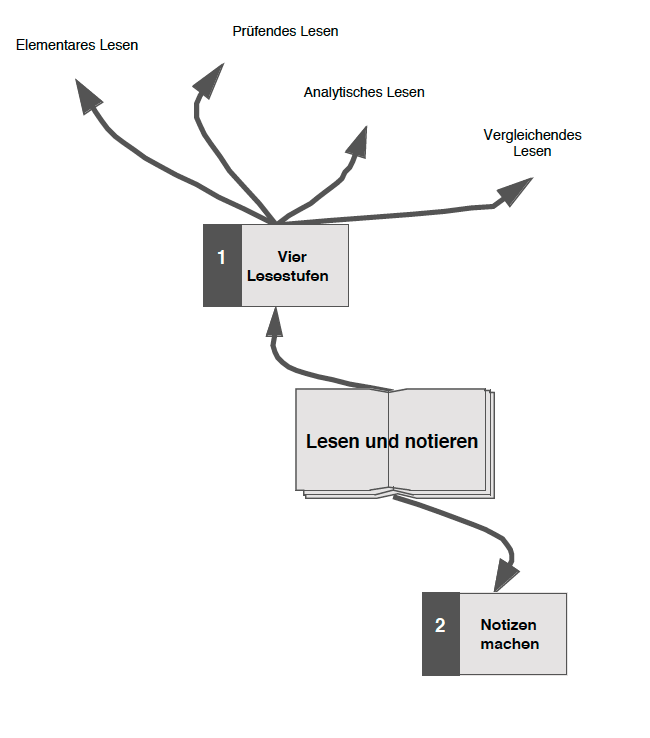
\includegraphics{images/lesen-min} 

}

\caption{Lesen (Überblick)}\label{fig:unnamed-chunk-15}
\end{figure}

Es gibt verschiedene Arten des Lesens, die wir alle kennen: wir lesen
Zeitungen anders als einen Krimi, und Gedichte anders als einen
Reiseführer. Die Unterscheidungen gehen aber noch weiter: Einen
Reiseführer lese ich zu Hause -- vor der Tour --, um schon etwas über
die Region zu erfahren, bevor ich hinfahre, um möglichst gut auf die
Reise vorbereitet zu sein. Während der Fahrt dagegen brauche ich den
Reiseführer für einen ganz bestimmten Zweck und suche mir daher nur mehr
heraus, was mir bei der Bewältigung der aktuellen Frage hilft (z. B. ein
gutes Restaurant finden).

\begin{figure}

{\centering 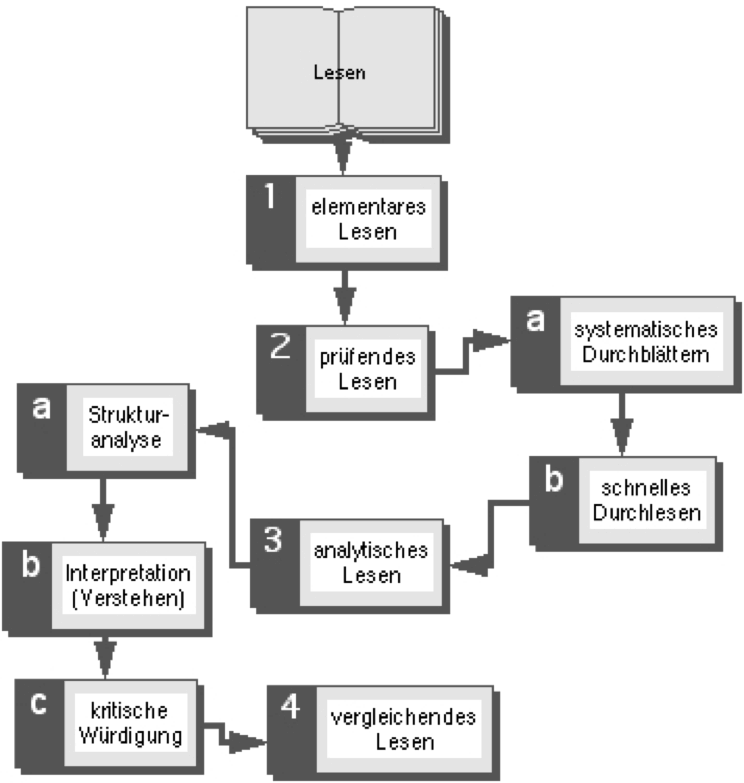
\includegraphics{images/lesen-4-stufen-min} 

}

\caption{Vier Lesestufen}\label{fig:unnamed-chunk-16}
\end{figure}

So wie es in den unterschiedlichen Phasen einer Reise (Vorbereitung,
Durchführung, Nachbereitung) verschiedene Interessen (und damit Ziele)
im Umgang mit einem Reiseführer gibt, so lassen sich auch beim Lesen
verschiedene Stufen unterscheiden. Der historische, aber immer noch
aktuelle ``Klassiker`` zur Kunst des Lesens, auf den wir uns hier in
diesem Kapitel stützen werden, unterscheidet sogar vier verschiedene
Ebenen im Lesevorgang. Auch wenn sie unterschiedliche Charakteristika
aufweisen, sind diese verschiedenen Stufen nicht unabhängig voneinander,
sondern bauen aufeinander auf: Jede höhere Stufe setzt die untere Stufe
voraus, d. h. baut auf ihr auf und schließt sie mit ein.

\section{Vier Lesestufen}\label{vier-lesestufen}

\subsection{Elementares Lesen}\label{elementares-lesen}

Warum sich überhaupt so ausführlich mit Lesen beschäftigen? Können wir
nicht davon ausgehen, dass wir alle in unserer Grundausbildung bereits
das Lesen ausreichend gelernt haben? Ja und nein. Wenn darunter bloß das
Lesen von Wörtern und Sätze verstanden wird, dann ja. Aber das wörtliche
Verstehen von Sätzen ist erst die erste Stufe im Prozess des Verstehens
eines Textes. Sie ist zwar die notwendige Basis, von der aus erst wir
uns ein tieferes Verständnis des Textes erarbeiten können. Sie ist aber
nur dann ausreichend, wenn es um Unterhaltung oder um bloße Aneignung
von Faktenwissen d. h. um statische Informationen geht.

Es ist wohl bezeichnend und alarmierend, dass wir in der heutigen
``Informationsgesellschaft`` dazu neigen, diese allererste Lesestufe mit
dem ganzheitlichen Leseprozess zu verwechseln. Obwohl zwar auch das
Elementare Lesen (z. B. beim Lesen einer Zeitung, beim Lesen eines
Buches zum Vergnügen im Urlaub usw.) seine eigene Berechtigung hat, ist
es zum Erarbeiten von wissenschaftlichen Texten zu wenig. Die wahre
Kunst des Lesens gibt sich nicht mit Einprägen (und Nachbeten) von
Fakten zufrieden, sondern beruht auf Verständnis, Einsicht und
Erkenntnis der Zusammenhänge.

Wir vermuten, dass gerade diese Verwechslung und das damit
zusammenhängende Missverständnis über den Charakter des Lesens für viele
Schwierigkeiten im wissenschaftlichen Schreibprozess mitverantwortlich
sind. Lesen und Schreiben -- so unsere These -- verhalten sich
komplementär zueinander. Weil viele Studierende sich (noch) nicht die
höheren Lesefertigkeiten angeeignet haben, können sie diese Fähigkeiten
beim Schreiben nicht umsetzen. Was beim Lesen meistens noch kaschiert
werden kann, tritt beim Schreiben offen zu Tage: Wo keine Zusammenhänge
verstanden oder Einsichten gewonnen wurden, können diese auch nicht in
einer schriftlichen Argumentation dargestellt werden. Unser
Prüfungssystem, das meist noch immer wesentlich auf Reproduzieren
ausgerichtet ist, belohnt noch dieses Stehenbleiben auf dem basalen
Leseniveau.

Lesen erschöpft sich nicht in einer Rezeption von Fakten, sondern
fordert eine aktive Auseinandersetzung. Schon die Aneignung von
Sachverhalten ist kein passiver Vorgang, sondern erfordert aktive
Anteilnahme (Aufmerksamkeit, Konzentration) und konstruktive mentale
Mitarbeit (Einordnung und Vernetzung in bestehendes Wissen). Dieser
Grundsatz einer aktiven Lesehaltung gilt für alle vier Lesestufen und
wird vor allem durch ständiges Fragen an den Text eingelöst.

Elementares Lesen als notwendige Basis wird in der Grundausbildung mehr
oder weniger gut vermittelt bzw. trainiert. Die anderen Lesestufen
hingegen fristen in unserem Bildungssystem leider ein Schattendasein:
Sie werden zwar beim selbständigen wissenschaftlichen Arbeiten
vorausgesetzt, aber kaum systematisch gelehrt oder geübt.

\subsection{Prüfendes Lesen}\label{prufendes-lesen}

Mit dieser zweiten Lesestufe beginnt erst die eigentliche Fertigkeit des
Erarbeitens bzw. Durcharbeitens eines Textes. Wir unterscheiden zwei
verschiedene Techniken des prüfenden Lesens, die bei geübten Leserinnen
bruchlos ineinander übergehen bzw. sich auch mehrmals abwechseln können:
systematisches Durchblättern und ein erstes schnelles Durchlesen. Ziel
beider Lesetechniken ist es, den Text einer gründlichen Inspektion zu
unterziehen. Es interessieren hierbei (noch) keine Details, sondern es
geht vorerst um eine grundlegende Orientierung: ist das Buch/der Artikel
für meine aktuellen Zwecke überhaupt nützlich?

Wissenschaftliche Arbeiten haben oft präzise und aussagekräftige
(Unter-)Titel. Titel, Untertitel und das schnell durchgelesene Vorwort
ermöglichen es Ihnen meistens bereits, Gebiet und Ziel des Textes sowie
die besondere Blickrichtung der Autorin zu erfassen.

Obwohl der Klappentext (aus Werbegründen) mit Vorsicht zu genießen ist,
wird er doch meist von der Autorin selbst (mit Hilfe der Public
Relations Abteilung des Verlags) erstellt. Vom Klappentext sollte sich
die Absicht, die die Autorin mit diesem Buch verfolgt, ablesen lassen.

Ein intensives Studium des Inhaltsverzeichnisses verschafft Ihnen einen
Überblick über Struktur und Gliederung des Textes. Vor allem die
Überschriften auf unteren Ebenen sind inhaltlich oft recht
aussagekräftig. An Hand des Umfangs der Untergliederungen und der
Seitenzahlen, die den einzelnen Kapiteln gewidmet sind, erkennen Sie
bereits die relative Wichtigkeit einzelner Themen.

Ähnliches gilt vom Sachregister: Hier sehen Sie nicht nur, welche
Begriffe vorkommen, sondern entnehmen (durch die Anzahl der
Seiteneinträge, der jeweiligen Gliederung in Unterbegriffe) auch ihre
relative Bedeutung für den gesamten Text.

Ein Überfliegen des Literaturverzeichnisses hilft Ihnen vor allem dann,
wenn Sie sich zum Thema schon ein wenig eingelesen haben: Kommen die
Ihnen wichtigen Arbeiten vor? Auf welche anderen Werke bezieht sich die
Autorin?

Besonders wichtig sind Zusammenfassungen. Sie sind oft typografisch oder
durch eigene Überschriften hervorgehoben und damit leicht zu finden.
Falls nicht, so müssen Sie auf den letzten paar Seiten des Buchs
(Kapitels) nach abschließenden Bemerkungen, Resumés, Schlussfolgerungen
etc. suchen.

Über Inhaltsverzeichnis oder Index können Sie interessante Passagen
heraussuchen und kurz probelesen. ``Erfühlen`` Sie den Herzschlag des
Buches: Wie ist es geschrieben? Worum geht es der Autorin? Wie packt die
Verfasserin die Probleme an?

Alle Materialien, die im Zuge der Literatursuche zusammengetragen
wurden, werden dieser raschen Prüfung unterzogen. Ergebnis ist die
Antwort auf die entscheidende Frage: Lohnt sich eine weitere
(intensivere) Beschäftigung mit dem Text? Um zu beurteilen, ob ein Text
für die aktuell verfolgte Fragestellung nutzbringend ist, muss er nicht
ausführlich und zeitraubend gelesen werden. Grundfragen sind: Um was
geht es? Welche Struktur, Teile hat der Text? Um welchen Texttyp handelt
es sich?

Das systematische Durchsehen eines Textes liefert aber weit mehr als
bloß eine Antwort auf die Frage zum weiteren Verfahren. Diese Lesestufe
setzt den Rahmen für alle weiteren Leseanstrengungen. Aus
Inhaltsverzeichnis, Sachregister und den kurzen Leseproben lassen sich
oft bereits viele inhaltliche Grundgedanken erfassen, die das weitere
Lesen steuern und erleichtern. Vielleicht braucht nur ein Teil des
Buches für meine besondere Themenstellung studiert zu werden? Soll
dieser Text sofort oder erst später -- nach Studium anderer Bücher --
gelesen werden?

Mit „Durchlesen`` ist hier ein wirklich nur oberflächliches, flüchtiges
Lesen gemeint. Unverständliche Begriffe werden nicht nachgeschlagen,
unverständliche Passagen werden übergangen. Auf Anmerkungen oder
Literaturhinweise wird keine Rücksicht genommen. Es genügt bei diesem
Lesen, bloß einen Teil zu verstehen. Ziel ist es, einen ersten
Gesamteindruck von dem Buch zu bekommen. Gleichzeitig werden jene Teile
oder Kapitel lokalisiert, die leichter oder schwieriger zu lesen, die
für das eigene Thema wichtig oder weniger wichtig sind, usw.

Bei vielen Büchern genügt dieses einmalige „Non-Stop``--Durchlesen. Das
ist der Fall, wenn der Text redundant ist oder doch weit weniger die
aktuelle Fragestellung als angenommen trifft. Schnelles Durchlesen des
kompletten Textes verhindert auch, dass ein falsches Bild durch
besonders ausgewählte Passagen entstehen kann: Das flüchtige Durchlesen
liefert den breiteren Zusammenhang und ermöglicht Überblick, Ein- und
Zuordnung der Position der Autorin und hilft bei der Erstellung des
genauen Leseplans (Reihenfolge, Prioritäten).

Für diese Art des Lesens sind schnelle Lesetechniken sehr vorteilhaft.
Verschiedene Methoden und Trainingskurse setzen hier an und helfen die
Lesegeschwindigkeit zu steigern. Meistens basieren sie auf der Korrektur
von Lesefehlern (Lippenbewegungen, Blickregressionen) und Übungen zur
Erweiterung der Blickspanne. Alleine eine willentlich größere
Lesegeschwindigkeit erhöht die Aufmerksamkeit und Konzentration und
damit meist auch die Behaltensleistung. So wichtig diese Techniken auch
für diese zweite Lesestufe sind, sie helfen nicht, wenn es darum geht,
Argumentstrukturen zu erkennen, zu verstehen und verarbeiten zu wollen.

\subsection{Analytisches Lesen}\label{analytisches-lesen}

Mit der dritten Lesestufe beginnt nun die eigentlich ``hohe`` Schule des
Lesens. Analytisches Lesen hat das Ziel, ein Werk zu verstehen, sich
damit auseinanderzusetzen, es kompetent bewerten zu können. Auch hier
lassen sich wieder verschiedene Phasen unterscheiden: Struktur-,
Interpretations- und Kritikphase. Die wichtigste Voraussetzung dafür
ist, mit bestimmten Fragen an das Buch heranzugehen und beim Lesen die
Antworten darauf zu suchen.

\begin{longtable}[]{@{}l@{}}
\caption{\textbf{\label{tab:analytisch-lesen} Analytisch lesen
(Übersicht)}}\tabularnewline
\toprule
\begin{minipage}[t]{0.97\columnwidth}\raggedright\strut
\begin{enumerate}
\def\labelenumi{\arabic{enumi}.}
\tightlist
\item
  \textbf{Fragen zur Struktur}
\end{enumerate}

\begin{itemize}
\tightlist
\item
  Um welche Art von Buch handelt es sich?
\item
  Was ist das Thema?
\item
  Wie wird dieses Thema abgehandelt?
\item
  Welche Fragen wirft die Autorin auf? Welche Probleme sollen gelöst
  werden? \vspace{-6mm}
\end{itemize}\strut
\end{minipage}\tabularnewline
\begin{minipage}[t]{0.97\columnwidth}\raggedright\strut
\begin{enumerate}
\def\labelenumi{\arabic{enumi}.}
\setcounter{enumi}{1}
\tightlist
\item
  \textbf{Fragen zur Interpretation}
\end{enumerate}

\begin{itemize}
\tightlist
\item
  Was wird im Detail genau gesagt?
\item
  Wie lautet genau die Argumentation?
\item
  Welche Antworten, Lösungsvorschläge gibt die Autorin?
\item
  Wie begründet sie diese?
\end{itemize}\strut
\end{minipage}\tabularnewline
\begin{minipage}[t]{0.97\columnwidth}\raggedright\strut
\begin{enumerate}
\def\labelenumi{\arabic{enumi}.}
\setcounter{enumi}{2}
\tightlist
\item
  \textbf{Fragen zur Kritik (I): Argumentation}
\end{enumerate}

\begin{itemize}
\tightlist
\item
  Wo stimme ich mit der Autorin überein?
\item
  Wo nicht?
\item
  Warum stimme ich -- bzw. stimme ich nicht -- mit der Autorin überein?
\item
  Wie stehe ich zu den Antworten bzw. Lösungen der Autorin?
\end{itemize}\strut
\end{minipage}\tabularnewline
\begin{minipage}[t]{0.97\columnwidth}\raggedright\strut
\begin{enumerate}
\def\labelenumi{\arabic{enumi}.}
\setcounter{enumi}{3}
\tightlist
\item
  \textbf{Fragen zur Kritik (II): Relevanz}
\end{enumerate}

\begin{itemize}
\tightlist
\item
  Was ist die Bedeutung des Buches?
\item
  Was ist neu, anders, relevant,\ldots{}?
\item
  Was folgt daraus?
\item
  Wie ist das Buch zu bewerten, einzuschätzen (Kritik, Würdigung,
  Enthaltung)?
\end{itemize}\strut
\end{minipage}\tabularnewline
\bottomrule
\end{longtable}

\begin{figure}

{\centering 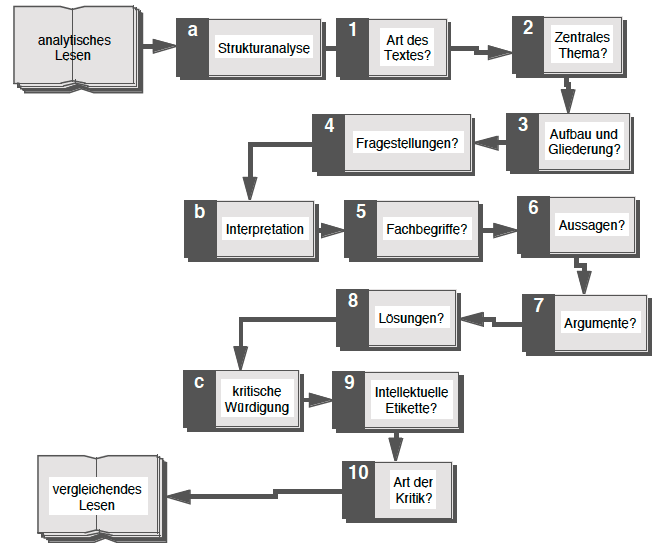
\includegraphics{images/lesen-analytisches-min} 

}

\caption{Prozess des analytischen Lesens}\label{fig:unnamed-chunk-17}
\end{figure}

Gegenüber der Vorgangsweise beim prüfenden Lesen gibt es wesentliche
Unterschiede: Beim Inspizieren überlappen bzw. vermischen sich teilweise
die beiden Phasen (systematisches Durchblättern und schnelles
Durchlesen) und die Reihenfolge der verschiedenen Schritte beim
Durchblättern ist relativ beliebig. Die drei Etappen wie auch die
einzelnen Schritte innerhalb jeder Phase des analytischen Lesens sind
jedoch als deutlich getrennte Arbeitsschritte aufzufassen, die weder
willkürlich vertauscht noch übersprungen werden können.

Bereits in der Vorbereitungsphase des prüfenden Lesens haben Sie wie ein
Detektiv Hinweise über Charakter und Struktur des Buches gesammelt. Nach
einem gründlichen Studium sollten Sie nun diese Vermutungen begründet
verwerfen oder bestätigen können. Ist es eine eher theoretische,
praktische oder empirische Arbeit? (siehe „Theoretische und praktische
Probleme``, S. †102) In welches Fachgebiet -- mit den jeweils
spezifischen Methoden -- ist das Buch einzuordnen (Geschichte,
Psychologie, Soziologie, Pädagogik,\ldots{})?

Was ist das zentrale Thema des Buches? Was ist die wesentliche
Fragestellung, der entscheidende Punkt? Hier genügt es nicht, bloß eine
vage Vorstellung zu haben: Fassen Sie den Hauptpunkt des Buches in einem
(kurzen!) Satz schriftlich zusammen. Sollte das nicht ausreichen, so
können Sie mit ein bis zwei weiteren Sätzen diesen Kernsatz noch weiter
spezifizieren.

Im dritten Schritt versuchen Sie nun, Aufbau und die Gliederung des
Buches unter diesem zentralen Gesichtspunkt schriftlich
zusammenzufassen. Thema und Gliederung bedingen sich wechselseitig: Erst
wenn Sie die Struktur deutlich sehen und mit dem zentralen Gehalt
verbinden können, wird Ihre kurze inhaltliche Zusammenfassung mit
Bedeutung gefüllt. Umgekehrt zieht Ihre (formale) Struktur aus der
thematischen Zusammenfassung ihre Substanz und gewinnt an Sinn.

Das Inhaltsverzeichnis kann Ihnen dabei -- muss aber nicht -- helfen: Es
kommt ganz auf Ihre Sichtweise, die Sie im Kernsatz formuliert haben,
an. Es gibt viele verschiedene Zugänge und/oder Perspektiven für ein
Buch. Jeder Text bedeutet für einen anderen Leser (je nach Interesse,
bisheriger Lebens- und/oder Lese-Erfahrung) etwas anderes. Auch wenn es
keine „richtige`` Lösung gibt, so sind Sie in Ihrer Zusammenfassung
selbstverständlich nicht völlig frei, sondern müssen Ihre Auffassung mit
dem Text selbst begründen.

Wenn Sie Ihre strukturelle Analyse gleich am Computer festhalten, können
Sie bereits eine Reihe guter Softwarehilfen verwenden. Der Vorteil
dieser Werkzeuge (``Outliner``; es handelt sich dabei entweder um
eigenständige Anwendungsprogramme oder um Funktionen von
Textverarbeitungsprogrammen) liegt nicht nur in der Gliederungshilfe
sondern auch darin, dass Sie verschiedene Sichtweisen (``Multiple
Representations``) auf Ihren Text haben. So können Sie Ihre Gliederung
nicht nur in verschiedenen Detaillierungsgraden betrachten, sondern bei
einigen Programmen auch grafisch darstellen. Die Software unterstützt so
nicht nur Ihre Aufgabe, sondern wird selbst zu einem Werkzeug der
Erkenntnis.

Diese ersten drei Untersuchungsschritte (Texttyp, Thema und Aufbau)
zusammengenommen, ergeben ein erstes Bild über Einheit, Klarheit und
Kohärenz des Buches. Die vierte Frage an den Text ist hingegen eine
Vorbereitung für die spätere Gesamtbeurteilung (Kritik, Würdigung) des
Werkes. Um welche Fragestellungen geht es im Buch? Welche Probleme
möchte die Autorin lösen? Es genügt hier nicht nur, die Fragestellungen,
die die Autorin verfolgt, aufzulisten, sondern es sind auch Reihenfolge
und Prioritäten wichtig.

Ganz allgemein lassen sich zwei Typen von Problemstellungen
unterscheiden:

\begin{itemize}
\tightlist
\item
  Theoretische Texte: Erkundungen über ein ``Objekt`` (darunter können
  auch geistige ``Dinge``, Begriffe etc. fallen).
\item
  Praktische Texte: Untersuchungen über Sinn, Zweck von Handlungen.
  (Analysen über Struktur, Eigenschaften oder Merkmale von Handlungen
  sind jedoch theoretische Texte.) Die Handlung ist selbst Gegenstand,
  die praktischen Probleme sind vor allem moralische bzw. ethische
  Fragestellungen. Dies zeigt sich auch darin, dass sie meistens mit
  ``soll`` eingeleitet werden.
\end{itemize}

\begin{longtable}[]{@{}l@{}}
\caption{\textbf{\label{tab:theoretische-texte} Allgemeine Fragen zu
theoretischen Texten}}\tabularnewline
\toprule
\begin{minipage}[t]{0.97\columnwidth}\raggedright\strut
\begin{itemize}
\tightlist
\item
  Wird die Existenz eines Objekts problematisiert? \vspace{-6mm}
\end{itemize}\strut
\end{minipage}\tabularnewline
\begin{minipage}[t]{0.97\columnwidth}\raggedright\strut
\begin{itemize}
\tightlist
\item
  Um welche Art von Objekt handelt es sich? \vspace{-6mm}
\end{itemize}\strut
\end{minipage}\tabularnewline
\begin{minipage}[t]{0.97\columnwidth}\raggedright\strut
\begin{itemize}
\tightlist
\item
  Was verursacht(e) seine Existenz? Warum? Unter welchen
  Voraussetzungen, Bedingungen kann es existieren? \vspace{-6mm}
\end{itemize}\strut
\end{minipage}\tabularnewline
\begin{minipage}[t]{0.97\columnwidth}\raggedright\strut
\begin{itemize}
\tightlist
\item
  Was verursacht(e) seine Existenz? Warum? Unter welchen
  Voraussetzungen, Bedingungen kann es existieren? \vspace{-6mm}
\end{itemize}\strut
\end{minipage}\tabularnewline
\begin{minipage}[t]{0.97\columnwidth}\raggedright\strut
\begin{itemize}
\tightlist
\item
  Welchem Zweck dient es? \vspace{-6mm}
\end{itemize}\strut
\end{minipage}\tabularnewline
\begin{minipage}[t]{0.97\columnwidth}\raggedright\strut
\begin{itemize}
\tightlist
\item
  Was sind die Konsequenzen seiner Existenz? \vspace{-6mm}
\end{itemize}\strut
\end{minipage}\tabularnewline
\begin{minipage}[t]{0.97\columnwidth}\raggedright\strut
\begin{itemize}
\tightlist
\item
  Was sind seine charakteristischen Eigenschaften, seine wesentlichen
  Merkmale? \vspace{-6mm}
\end{itemize}\strut
\end{minipage}\tabularnewline
\begin{minipage}[t]{0.97\columnwidth}\raggedright\strut
\begin{itemize}
\tightlist
\item
  Welche Beziehung hat das Objekt zu anderen Objekten seiner bzw.
  anderer Art? \vspace{-6mm}
\end{itemize}\strut
\end{minipage}\tabularnewline
\begin{minipage}[t]{0.97\columnwidth}\raggedright\strut
\begin{itemize}
\tightlist
\item
  Wie verhält es sich (unter bestimmten Bedingungen)?
\end{itemize}\strut
\end{minipage}\tabularnewline
\bottomrule
\end{longtable}

\begin{longtable}[]{@{}l@{}}
\caption{\textbf{\label{tab:praktische-texte} Allgemeine Fragen zu
praktischen Texten}}\tabularnewline
\toprule
\begin{minipage}[t]{0.97\columnwidth}\raggedright\strut
\begin{itemize}
\tightlist
\item
  Welche Ziele sollten verfolgt werden? \vspace{-6mm}
\end{itemize}\strut
\end{minipage}\tabularnewline
\begin{minipage}[t]{0.97\columnwidth}\raggedright\strut
\begin{itemize}
\tightlist
\item
  Welche Mittel sollten für einen bestimmten Zweck verfolgt werden?
  \vspace{-6mm}
\end{itemize}\strut
\end{minipage}\tabularnewline
\begin{minipage}[t]{0.97\columnwidth}\raggedright\strut
\begin{itemize}
\tightlist
\item
  Was muss getan werden, um ein bestimmtes Ziel erreichen zu können?
  \vspace{-6mm}
\end{itemize}\strut
\end{minipage}\tabularnewline
\begin{minipage}[t]{0.97\columnwidth}\raggedright\strut
\begin{itemize}
\tightlist
\item
  In welcher Reihenfolge muss dazu vorgegangen werden? \vspace{-6mm}
\end{itemize}\strut
\end{minipage}\tabularnewline
\begin{minipage}[t]{0.97\columnwidth}\raggedright\strut
\begin{itemize}
\tightlist
\item
  Unter den aktuellen Bedingungen: Was ist das Beste, das Optimale, das
  mit dem geringsten Schaden, was gemacht werden kann? \vspace{-6mm}
\end{itemize}\strut
\end{minipage}\tabularnewline
\begin{minipage}[t]{0.97\columnwidth}\raggedright\strut
\begin{itemize}
\tightlist
\item
  Unter welchen (anderen) Bedingungen wäre es besser, schlechter?
\end{itemize}\strut
\end{minipage}\tabularnewline
\bottomrule
\end{longtable}

Die Interpretation ist sowohl in der analytischen Lesestufe als auch für
die Lesefertigkeit insgesamt die große Bewährungsprobe. Hier liegt der
eigentliche Kern des Verstehensprozesses. Gleichzeitig ist die durch die
Textauslegung gewonnene Einsicht wohl auch jene Fähigkeit innerhalb der
komplexen Lesefertigkeit, die am schwierigsten anzueignen ist. Das liegt
einerseits am Vorwissen: Gute sprachliche Kenntnisse (Wortschatz,
Grammatik, Satzstrukturen) sind eine notwendige Grundvoraussetzung,
Vertrautheit mit logischen Figuren im Alltag (``informelle Logik``:
Erkennen von Propositionen und Argumenten, Einschätzung der Qualität
einer Argumentationsstruktur) sehr hilfreich.

Andererseits aber ist der -- im Prozess der Interpretation notwendige --
hermeneutische Zirkel (Hermeneutik = Kunst der (Text-)Auslegung) selbst
ein Grund für diese Schwierigkeit: im Erkenntnisprozess bzw. beim
Verstehen gehen wir immer von einem (geschichtlichen) Vorverständnis
aus, von dem her wir die Welt (den Text) auslegen. In der aktiven
Auseinandersetzung wird dieses Vorurteil abgewandelt, modifiziert und
erweitert. Dieses neue Verständnis wird bei einer neuerlichen Deutung
zum neuen Vorverständnis (Vorurteil) der Interpretation. Unser
Verstehensprozess ist daher zirkulär aufgebaut.

Diese lange geisteswissenschaftliche Tradition der Textauslegung können
wir hier natürlich nicht referieren. Wir werden -- trotz dieser
traditionsschweren und komplexen Hintergründe -- versuchen, relativ
unbekümmert einige Hilfestellungen für die tägliche Lesepraxis so
darzulegen, dass sie zwar ihre theoretische Herkunft nicht ganz leugnen,
aber dennoch verständlich und vor allem praxisrelevant sind.

Eine der wichtigsten Regeln bei der Textauslegung lautet: Verständigen
Sie sich mit der Autorin über die Verwendung der zentralen Fachbegriffe!
Es geht darum, dass Sie den grundlegenden Ausdrücken im Text jene
Bedeutung zuschreiben, wie sie die Autorin selbst versteht, bzw.
intendiert hat. Das ist ganz und gar keine leichte Aufgabe:

Einerseits können dieselben Worte unterschiedliche Bedeutungen haben.
Gemeint ist hier nicht bloß der triviale Fall eines gänzlich
unterschiedlichen Sinnzusammenhangs (wie z. B. bei ``ein Buch lesen``
und ``Wein lesen``), sondern die Schwierigkeit besteht vor allem in der
Nuancierung des begrifflichen Inhalts und Bedeutungsumfanges (wie z. B.
``lesen`` als Informationsaufnahme und als Gewinnung von Einsichten).

Andererseits drücken verschiedene Wörter oft gleiche Bedeutungen aus
(Synonyme). Wiederum ist die Sache nicht so einfach wie es scheint:
Lediglich in wenigen Fällen gibt es eine völlige Übereinstimmung (totale
Synonymie wie z. B. bei ``Fleischer`` und ``Metzger``); meistens haben
wir es nur mit einer Sinnverwandtschaft (partielle Synonymie wie z. B.
bei Freude, Frohsinn, Vergnügen,\ldots{}) zu tun.

Manchmal kann dieser Einigungsprozess auch durch den Autor selbst
erschwert werden, z. B. wenn er seine zentralen Begriffe entweder nicht
klar abgrenzt und eindeutig verwendet. Das ist dann aber gleich selbst
ein wichtiger Hinweis auf die später zu führende Kritik.

Wie können Sie das Ziel einer Verständigung mit der Begriffswelt der
Autorin erreichen? In den meisten Fällen können Sie nicht die Autorin
selbst fragen, sondern müssen die Interpretation aus dem Text selbst
erschließen. Es wirkt hier wieder der bereits erwähnte hermeneutische
Zirkel (vgl. Seite†103): Die umliegenden Wörter und Sätze bilden den
Kontext für den zu interpretierenden Begriff. Sie erschließen seine
Bedeutung aus diesem Kontext, indem Sie Ihr (Vor-)Verständnis jener
Wörter und Ausdrücke anwenden, die Sie bereits kennen, bzw. zu kennen
glauben. Es ist wie ein Puzzlespiel nach der Methode von Versuch und
Irrtum: Sie wenden Ihr Vorverständnis an und gewinnen neue Einsichten,
die Sie wiederum anwenden. Je weiter Sie voranschreiten, desto klarer
wird das Bild werden. Manchmal müssen Sie vielleicht wieder zurück und
Änderungen vornehmen, an die Sie jedoch bereits mit einem anderen
Verständnis herangehen können als zu Beginn der Auslegung.

Obwohl es keine zwingenden Algorithmen für die Vorgangsweise gibt,
lassen sich doch einige heuristische Hilfen (Daumenregeln) anführen:
Ihre erste Aufgabe im Prozess der Interpretation muss es sein, die
entscheidenden Fachbegriffe ausfindig zu machen:

\begin{longtable}[]{@{}l@{}}
\caption{\textbf{\label{tab:schluesselbegriffe} Hilfen zum Auffinden der
Schlüsselbegriffe}}\tabularnewline
\toprule
\begin{minipage}[t]{0.97\columnwidth}\raggedright\strut
\begin{itemize}
\tightlist
\item
  Gibt es Begriffe, die Ihnen (auch nachdem Sie ein Lexikon konsultiert
  haben) noch Verständigungsprobleme machen? \vspace{-6mm}
\end{itemize}\strut
\end{minipage}\tabularnewline
\begin{minipage}[t]{0.97\columnwidth}\raggedright\strut
\begin{itemize}
\tightlist
\item
  Gibt es Begriffe, die die Autorin besonders hervorhebt (kursiv,
  Anführungszeichen)? \vspace{-6mm}
\end{itemize}\strut
\end{minipage}\tabularnewline
\begin{minipage}[t]{0.97\columnwidth}\raggedright\strut
\begin{itemize}
\tightlist
\item
  Gibt es Begriffe, die die Autorin (in Auseinandersetzung mit anderen
  Autoren) ausführlich diskutiert? \vspace{-6mm}
\end{itemize}\strut
\end{minipage}\tabularnewline
\begin{minipage}[t]{0.97\columnwidth}\raggedright\strut
\begin{itemize}
\tightlist
\item
  Gibt es im Index Begriffe, unter denen lange Ketten von Eintragungen
  und/oder viele Unterbegriffe stehen? \vspace{-6mm}
\end{itemize}\strut
\end{minipage}\tabularnewline
\begin{minipage}[t]{0.97\columnwidth}\raggedright\strut
\begin{itemize}
\tightlist
\item
  Gibt es Begriffe, die in einem zuständigen Fachlexikon ausführlich
  abgehandelt werden? \vspace{-6mm}
\end{itemize}\strut
\end{minipage}\tabularnewline
\begin{minipage}[t]{0.97\columnwidth}\raggedright\strut
\begin{itemize}
\tightlist
\item
  Welche Begriffe werden synonym verwendet, mit welchem Gehalt? (Machen
  Sie sich zwei Listen: In eine schreiben Sie die von der Autorin
  verwendeten Wörter, in die andere, die dazugehörige Bedeutung. Danach
  vergleichen Sie.)
\end{itemize}\strut
\end{minipage}\tabularnewline
\bottomrule
\end{longtable}

Ein ähnliches Problem taucht beim nächsten Schritt der Entwicklung der
Interpretation auf: Es geht nun darum, sich mit der Autorin über die von
ihr geäußerten Gedanken und Aussagen ins Einvernehmen zu setzen.
Wiederum muss zwischen der sprachlichen und der logischen Ebene
unterschieden werden. Wiederum besteht zwischen den (formalen)
sprachlichen Elementen (Sätze und Absätze) und den (logischen)
inhaltlichen Bestandteilen (Propositionen oder Aussagen und Argumente)
keine 1:1-Relation.

Im Satz ``Es ist allgemein bekannt, dass die Erde rund ist``, lautet die
darin enthaltene Proposition ``Die Erde ist rund``. Im Satz: ``Die Erde
ist rund und überbevölkert`` finden wir hingegen sogar zwei
Propositionen. Umgekehrt können sich (logische) Aussagen auch über
mehrere (Ab-)Sätze verteilen. Propositionen sind die Grundeinheiten für
Gedanken und Wissensstrukturen. Sie sind Deklarationen des Wissens (der
Meinung, der Vermutung, der Befürchtung,\ldots{}) Propositionen stellen
die Antwort zu (nicht immer explizierten) Fragestellungen dar: ``Welche
Merkmale hat die Erde?``

Wir haben es auf dieser zweiten Etappe des analytischen Leseprozesses
mit einer gegenläufigen Bewegung zur ersten Phase zu tun. Beide
Teilstücke treffen hier zusammen:

\begin{itemize}
\tightlist
\item
  Struktur: Vom Buch als Ganzes über die einzelnen Abschnitte und
  Kapitel zu den Argumentationen und Aussagen.
\item
  Interpretation: Von den einzelnen Fachbegriffen über die zentralen
  Sätze zu den Aussagen und Argumentationen.
\end{itemize}

Wiederum geht es zuerst darum, die zentralen Gedanken des Textes
ausfindig zu machen. Eine wichtige heuristische Hilfe dabei ist die
Suche nach Schlüsselsätzen. Oft verbirgt sich in einem zentralen
sprachlichen Element auch ein wichtiger Gedanke. Oder anders herum: Der
betreffende Satz ist deshalb so wichtig, weil er einen grundlegenden
Gedanken formuliert. Vermeiden Sie dabei die Ablenkung durch
``interessante`` Sätze. Es geht hier (noch) nicht darum, was Sie
interessiert, sondern ob der Gedanke für das Grundthema des Textes von
besonderer Bedeutung ist. Viel wichtiger als wissenswerte und
aufschlussreiche Sätze sind ungewöhnliche, erstaunliche, überraschende
oder gar befremdliche Aussagen. (``Staunen ist der Beginn aller
Weisheit``).

\begin{longtable}[]{@{}l@{}}
\caption{\textbf{\label{tab:schluesselsaetze} Hilfen zum Auffinden der
Schlüsselsätze}}\tabularnewline
\toprule
\begin{minipage}[t]{0.97\columnwidth}\raggedright\strut
\begin{itemize}
\tightlist
\item
  Gibt es Sätze, die gerade wegen eines -- von Ihnen bereits
  aufgefundenen -- Schlüsselwortes eine zentrale Stellung im Text
  einnehmen? \vspace{-6mm}
\end{itemize}\strut
\end{minipage}\tabularnewline
\begin{minipage}[t]{0.97\columnwidth}\raggedright\strut
\begin{itemize}
\tightlist
\item
  Gibt es Sätze, die Ihnen (auch nachdem Sie ein Lexikon für einzelne
  Begriffe konsultiert haben) noch immer Verständnisprobleme machen?
  \vspace{-6mm}
\end{itemize}\strut
\end{minipage}\tabularnewline
\begin{minipage}[t]{0.97\columnwidth}\raggedright\strut
\begin{itemize}
\tightlist
\item
  Gibt es Sätze, die die Autorin besonders hervorhebt (kursiv,
  unterstrichen)? \vspace{-6mm}
\end{itemize}\strut
\end{minipage}\tabularnewline
\begin{minipage}[t]{0.97\columnwidth}\raggedright\strut
\begin{itemize}
\tightlist
\item
  Gibt es Sätze, über die Sie sich wundern? \vspace{-6mm}
\end{itemize}\strut
\end{minipage}\tabularnewline
\begin{minipage}[t]{0.97\columnwidth}\raggedright\strut
\begin{itemize}
\tightlist
\item
  Gibt es Sätze, die direkt das Hauptthema betreffen, es entweder
  spezifizieren (Prämisse) oder bewerten (Schlußfolgerung)?
  \vspace{-6mm}
\end{itemize}\strut
\end{minipage}\tabularnewline
\begin{minipage}[t]{0.97\columnwidth}\raggedright\strut
\begin{itemize}
\tightlist
\item
  Gibt es Sätze, von denen Sie bereits wissen, dass sie von anderen
  Autorinnen zitiert werden?
\end{itemize}\strut
\end{minipage}\tabularnewline
\bottomrule
\end{longtable}

Selbst wenn Sie die Schlüsselsätze gefunden und die darin enthaltenen
Propositionen lokalisiert haben, bleibt noch die wichtige und alles
entscheidende Frage offen. Haben Sie diese Aussagen auch verstanden?
Verstehen ist ein aktiver kognitiver Prozess, der von Ihnen selbst
geleistet werden muss und zu dem es keine endgültigen und vollständigen
Hilfen gibt. Was dieses Buch dazu anbieten kann, sind lediglich zwei
Kontrollen, die Ihnen anzeigen, ob Sie einen Sachverhalt verstanden
haben oder nicht. Diese Tests sind gleichzeitig auch zwei wertvolle
Übungen, die Ihnen auch helfen, den Text zu erarbeiten (zu verstehen):

Versuchen Sie den Sachverhalt mit eigenen Worten zu rekapitulieren. Wenn
Sie sich stark an den Originalwortlaut anlehnen müssen, so ist dies ein
Indiz dafür, dass Sie den Text nicht vollständig verstanden haben. Sie
können dann wahrscheinlich noch nicht zwischen spezifischen sprachlichen
Formulierungen und dem eigentlichen Sachverhalt unterscheiden.

Versuchen Sie den Sachverhalt mit eigenen Beispielen zu belegen oder zu
erweitern. Propositionen sind nicht formallogische Gebilde, sondern
Deklarationen über die Welt. Sie sollten daher in der Lage sein, diese
Aussagen umzusetzen, bzw. anzuwenden. Ihre Beispiele müssen nicht
unbedingt nur aus eigener Erfahrung oder der Ihnen bekannten
Lebenspraxis anderer Leute stammen, sondern Sie können sie auch
konstruieren oder erfinden.

Der nächste, vielleicht wichtigste, Schritt besteht darin, die von der
Autorin geäußerten Argumente herauszufinden. Dazu müssen Sie sowohl die
argumentativen Passagen herausfinden als auch jenen Stellen, die zwar
Gründe anführen, aber keine Argumentationen enthalten. Dazu wiederum ist
es notwendig genau zu wissen, was ein Argument ist und wodurch es sich
von anderen Textabschnitten (Erklärung, Beschreibung,\ldots{})
unterscheidet.

Das Auffinden von Prämissen und Schlussfolgerungen (die beiden
wesentlichen Bestandteile von Argumenten) ist eine komplexe Fähigkeit,
aber Voraussetzung dafür, dass Sie bei der nachfolgenden Kritikphase des
analytischen Lesens auch selbst beurteilen können, ob es sich um gute
oder schlechte Argumentationen handelt.

Nach der intensiven Vorarbeit sollte es Ihnen nun nicht mehr
schwerfallen, die Lösungsvorschläge der Autorin aufzulisten. Für welche
Probleme, die die Autorin angetreten ist zu klären, kann sie tatsächlich
eine Lösung anbieten? Und worin besteht sie? Für welche eingangs
erwähnten Fragestellungen hingegen wurden keine (befriedigende)
Antworten gegeben? Weiß der Autor, bei welchen Schwierigkeiten er
gescheitert ist und warum?

Bis hierher sind Sie den Spuren der Autorin gefolgt. Nach der
schwierigen Vorarbeit der Interpretation müssen Sie nun auf eigenen
Wegen wandeln und Ihre eigene Meinung entwickeln, äußern und begründen.
Aktives Lesen heißt nicht nur einen Text zu verstehen, sondern ihn auch
kritisch zu würdigen und zu beurteilen.

Gleich von vornherein wollen wir ein häufiges Missverständnis vermeiden:
Kritik heißt nicht bloß, Gegenargumente einzuwenden, und schon gar
nicht, einen Text schlecht zu machen oder abzuwerten. Kritik in unserem
Kontext bedeutet Stellung beziehen, eine Wertung, Einschätzung,
Beurteilung vornehmen. Das Ergebnis kann sowohl positiv als auch negativ
ausfallen, immer aber beruht es auf Begründungen. Kritisieren ist selbst
eine komplizierte Fähigkeit und beruht auf so unterschiedlichen
Tätigkeiten wie: abschätzen, bedenken, erwägen, gegenüberstellen,
überlegen, prüfen,\ldots{}

Ein Buch aktiv zu lesen, heißt eine Art von Kommunikation (mit der
Autorin) zu führen. Dieser Diskurs muss jedoch besonders behutsam
geführt werden, weil die Autorin nicht präsent ist und daher weder
Missverständnisse aufklären noch Gegenargumente replizieren kann. Als
aktive Leserin haben Sie (in Ihren Notizen) immer das letzte Wort.

Aus all diesen Gründen ist es wichtig, dass Sie ein bestimmtes
Mindestmaß an intellektuellen Umgangsformen beachten. Diese
Anstandsregeln sind nicht nur Gebote der sozialen Höflichkeit, sondern
helfen auch, eine Kommunikation effizient zu führen. Vor allem aber sind
es weitere Hilfen zur Verständigung mit der Autorin, die Sie vor
Fehlurteilen bewahren sollen.

\begin{longtable}[]{@{}l@{}}
\caption{\textbf{\label{tab:etikette} Regeln der intellektuellen
Etikette}}\tabularnewline
\toprule
\begin{minipage}[t]{0.97\columnwidth}\raggedright\strut
\begin{itemize}
\tightlist
\item
  Beginnen Sie erst mit der Kritik, wenn Sie die anderen Phasen des
  analytischen Lesens (Erfassung der Struktur und Interpretation)
  abgeschlossen haben \vspace{-6mm}
\end{itemize}\strut
\end{minipage}\tabularnewline
\begin{minipage}[t]{0.97\columnwidth}\raggedright\strut
\begin{itemize}
\tightlist
\item
  Beginnen Sie erst mit der Kritik, wenn Sie sicher sind, dass Sie den
  Text verstanden haben. (siehe „Zwei Verständniskontrollen``, S. 106)
  XXX \vspace{-6mm}
\end{itemize}\strut
\end{minipage}\tabularnewline
\begin{minipage}[t]{0.97\columnwidth}\raggedright\strut
\begin{itemize}
\tightlist
\item
  Vermeiden Sie Angriffe auf die Person, konzentrieren Sie sich auf die
  inhaltliche Ebene. \vspace{-6mm}
\end{itemize}\strut
\end{minipage}\tabularnewline
\begin{minipage}[t]{0.97\columnwidth}\raggedright\strut
\begin{itemize}
\tightlist
\item
  Respektieren Sie die Meinungen der Autorin und unterscheiden Sie
  zwischen persönlichen Auffassungen (Weltbildern) und rationalen
  Argumentationen. \vspace{-6mm}
\end{itemize}\strut
\end{minipage}\tabularnewline
\begin{minipage}[t]{0.97\columnwidth}\raggedright\strut
\begin{itemize}
\tightlist
\item
  Gehen Sie nicht mit einer abwertenden Haltung an den Text heran,
  sondern versuchen Sie, die Sachlage mit einer neutralen, bzw. sogar
  mit einer leicht positiven (sympathisierenden, wohlwollenden)
  Grundhaltung aus der Sicht der Autorin zu betrachten. \vspace{-6mm}
\end{itemize}\strut
\end{minipage}\tabularnewline
\begin{minipage}[t]{0.97\columnwidth}\raggedright\strut
\begin{itemize}
\tightlist
\item
  Halten Sie dem Autor bei einer negativen Bewertung ``mildernde
  Umstände`` zugute: Stand der damaligen Erkenntnisse, limitierte
  Möglichkeiten und Ressourcen (Zeit, Geld,\ldots{}), mangelnde
  wissenschaftliche Erfahrung,\ldots{} \vspace{-6mm}
\end{itemize}\strut
\end{minipage}\tabularnewline
\begin{minipage}[t]{0.97\columnwidth}\raggedright\strut
\begin{itemize}
\tightlist
\item
  Machen Sie Ihre eigenen Annahmen (Prämissen) explizit. (Eine gute
  Kontroverse ist ein Disput über unterschiedliche Schlussfolgerungen
  und nicht über unterschiedliche Voraussetzungen.) \vspace{-6mm}
\end{itemize}\strut
\end{minipage}\tabularnewline
\begin{minipage}[t]{0.97\columnwidth}\raggedright\strut
\begin{itemize}
\tightlist
\item
  Begnügen Sie sich nicht mit einer Ablehnung von Prämissen, sondern
  verfolgen Sie die Gedankengänge (Schlussfolgerungen) der Autorin und
  prüfen Sie deren interne Konsistenz, Klarheit und Stichhaltigkeit (bei
  gegebenen Prämissen). \vspace{-6mm}
\end{itemize}\strut
\end{minipage}\tabularnewline
\begin{minipage}[t]{0.97\columnwidth}\raggedright\strut
\begin{itemize}
\tightlist
\item
  Lernen Sie Ihre eigenen (positive wie negative) Emotionen kennen, die
  Sie bei einer bestimmten Auseinandersetzung (Disput) entwickeln.
  Akzeptieren Sie Ihre Gefühle aber halten Sie sie von Ihrer eigenen
  Argumentation getrennt.
\end{itemize}\strut
\end{minipage}\tabularnewline
\bottomrule
\end{longtable}

Es gibt sieben grundsätzliche Wege der Kritik. Allgemein gilt dabei:
Jegliche Art von Kritik muss auf dem Verständnis des Textes beruhen und
daher auch begründet werden. Das trifft ganz besonders auf die
Spezialfälle (Zustimmung, Enthaltung, Unverstehen) zu: ``Zuzustimmen
ohne zu verstehen, ist geistlos. Aber nicht zuzustimmen ohne zu
verstehen, ist unverschämt.`` (Adler/Doren 1972:143)

\subsection{Vergleichendes Lesen}\label{vergleichendes-lesen}

Bei dieser Lesestufe geht es nun nicht mehr darum, ein einzelnes Buch zu
erarbeiten, sondern um die Konstruktion eigener Argumente und Aussagen
im Diskurs mit mehreren relevanten Werken. Prüfendes Lesen war die
Vorbereitung für die analytische Lesestufe. Jetzt -- nachdem Sie mehrere
Bücher zum selben Thema analytisch erarbeitet haben -- wissen Sie,
welche Bücher (bzw. welche Passagen) zum selben Thema für Sie relevant
sind. Erst mit diesem Vorverständnis macht das vergleichende Lesen Sinn.

Syntopisches Lesen, wie das vergleichende Lesen auch heißt, ist im
Wesentlichen ein selektives Lesen. Durch die vorhergehenden Phasen des
Lesens unterstützt, sollen im ersten Schritt die relevanten Stellen
aufgefunden werden. Dieses selektive Lesen hat nun jedoch einen ganz
anderen Charakter als das - ebenfalls selektive - prüfende Lesen. Zu
inspizieren, ob ein Buch relevant ist, ist nicht gleichzusetzen mit dem
Auffinden relevanter Passagen in einem Buch. Für geübte Leser mögen
vielleicht diese verschiedenen Tätigkeiten ineinander übergehen; vor
einem kompletten Überspringen der analytischen Lesestufe muss jedoch
gewarnt werden.

\begin{figure}

{\centering 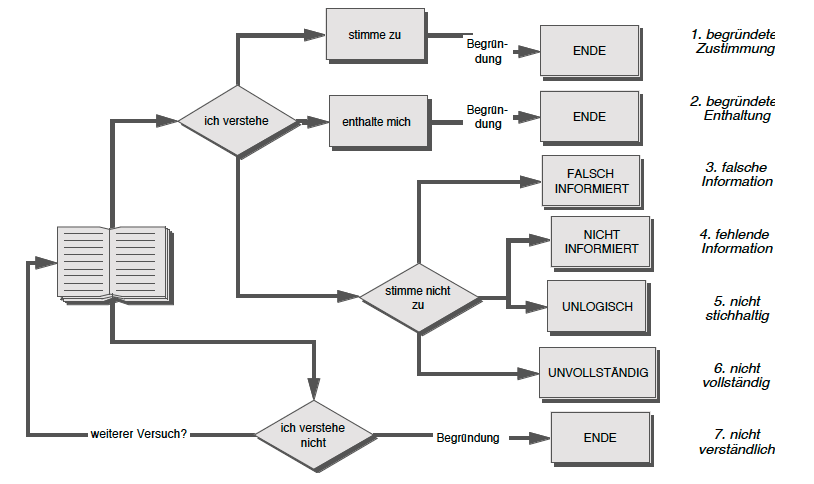
\includegraphics{images/lesen-vergleichendes-min} 

}

\caption{Vergleichendes Lesen}\label{fig:unnamed-chunk-18}
\end{figure}

Warum? Wieder ist der bereits mehrmals erwähnte hermeneutische Zirkel
(vgl. Seite 94) dafür verantwortlich: Wie können Sie wissen, ob beide
Bücher relevante Stellen zum selben Thema haben? Dazu müssten Sie
bereits das Thema vor dem Lesen identifizieren bzw. spezifizieren
können. Das aber ist oft erst nach dem analytischen Lesen, wo Sie sich
mit der Autorin über Thematik und Fragestellung ins detaillierte
Einvernehmen setzen, möglich.

Während Sie beim analytischen Lesen den Spuren der Autorin folgen, gehen
Sie beim syntopischen Lesen von Ihrem eigenen Interesse und Thema aus.
Sie suchen eine Textpassage nicht danach aus, ob und wie weit sie Ihnen
zum Verständnis des Buches hilft, sondern ob sie Ihnen bei der
Bearbeitung Ihrer eigenen Fragestellung helfen kann. Und das kann sich
durchaus stark von der Intention der Autorin unterscheiden.

Wie bei Stufe 5 (Seite 104 XXX) des analytischen Lesens müssen Sie sich
auch beim vergleichenden Lesen über die Bedeutung der Fachbegriffe
verständigen. Da Sie es aber nun mit mehreren Autorinnen gleichzeitig zu
tun haben, sind Sie es selbst, die die Grundlage für eine gemeinsame
Verständigung schaffen müssen. Statt herauszufinden, welche Bedeutung
der Begriff für die Autorin hat, müssen Sie die Autorin von Ihrer
eigenen Sprachverwendung ausgehend interpretieren. Syntopisches Lesen
ist wesentlich eine Übersetzungsprozedur: Sie (re)konstruieren den
Gedankengang der Autorin (der Autorinnen) vor dem Hintergrund Ihrer
eigenen Sinnzusammenhänge.

Weil Sie mit mehreren Autorinnen gleichzeitig in einen Diskurs treten
wollen, ist es notwendig, dass Sie eine eigene Sprache (eigene
Begrifflichkeiten, eigene Bedeutungszusammenhänge) zur Verständigung
entwickeln. Diese übergreifende Sprache muss systematisch entwickelt und
begründet werden, damit sie als ``neutrale`` Kommunikationsgrundlage
akzeptabel ist.

Im nächsten Schritt verwenden Sie nun den entwickelten begrifflichen
Apparat, die von Ihnen geschaffene Terminologie, um das Thema, zu dem
die verschiedenen Autorinnen diskutieren, neu zu definieren. Das ist
notwendig, weil Unterschiede in der Frage- bzw. Problemstellung der
verschiedenen Diskurspartner auf unterschiedliche theoretische Gerüste
zurückzuführen sind.

Von dieser Grundlage aus können Sie nun mit den Autorinnen in einen
wissenschaftlichen Diskurs treten. Sie übernehmen dabei die Rolle einer
Moderatorin: Sie geben das Thema vor, sehen zu, dass alle
Teilnehmerinnen an dieser virtuellen Diskussion zu Wort kommen, klären
Missverständnisse, verweisen auf Gemeinsamkeiten und halten
unterschiedliche Positionen fest. Dabei kehren Sie immer wieder zu den
Originaltexten zurück und lesen erneut die entsprechenden Passagen.

Wichtig bei diesem virtuellen Disput ist es, dass immer klar ist, um
welche Meinung es sich handelt. Im Fortgang dieser Auseinandersetzung
ist es oft sinnvoll, die eigene Position immer stärker einzubringen
(Rollenwechsel: Von der Moderatorin zur Diskutantin). Daher müssen Sie
klarmachen, was Ihre eigenen Worte und was die Beiträge der anderen
Teilnehmerinnen sind. Darin liegt der eigentliche Sinn der Regeln für
den Umgang mit Quellen beim wissenschaftlichen Schreiben (s. XXX Kapitel
„Zitieren``).

\section{Notizen machen}\label{notizen-machen}

Abschließend wollen wir die „technische Seite`` des Lesens von Texten
noch etwas genauer betrachten: es geht dabei um Hilfsmittel und
-tätigkeiten wie Markieren, Notieren und Exzerpieren.

Analytisches Lesen wird unterstützt dadurch, dass man einen Text auch
sichtbar und physisch „bearbeitet``, also durch Anstreichen und
Anmerkungen. Das ist natürlich nur in eigenen Büchern erlaubt. Bei
fremden, entliehenen Büchern muss man sich mit Notizen und Exzerpten auf
Notizblättern, Karteikarten usw. begnügen, oder man fertigt Kopien der
für die eigene Arbeit zentralen Teile an. Es hilft, wenn man sich schon
vor dem Lesen ein bestimmtes Instrumentarium an Markierungen und Notizen
zurechtlegt, zum Beispiel:

\begin{longtable}[]{@{}lll@{}}
\caption{\textbf{\label{tab:markieren-eigenes-buch} Markieren (eigenes
Buch)}}\tabularnewline
\toprule
\begin{minipage}[b]{0.31\columnwidth}\raggedright\strut
Sie verwenden \ldots{}\strut
\end{minipage} & \begin{minipage}[b]{0.27\columnwidth}\raggedright\strut
um\ldots{}\strut
\end{minipage} & \begin{minipage}[b]{0.33\columnwidth}\raggedright\strut
mögliche Probleme\strut
\end{minipage}\tabularnewline
\midrule
\endfirsthead
\toprule
\begin{minipage}[b]{0.31\columnwidth}\raggedright\strut
Sie verwenden \ldots{}\strut
\end{minipage} & \begin{minipage}[b]{0.27\columnwidth}\raggedright\strut
um\ldots{}\strut
\end{minipage} & \begin{minipage}[b]{0.33\columnwidth}\raggedright\strut
mögliche Probleme\strut
\end{minipage}\tabularnewline
\midrule
\endhead
\begin{minipage}[t]{0.31\columnwidth}\raggedright\strut
Unterstreichungen (auch in verschiedenen Farben)\strut
\end{minipage} & \begin{minipage}[t]{0.27\columnwidth}\raggedright\strut
wichtige Aussagen (Sätze) hervorzuheben; Stellen für Zitate
vorzumerken\strut
\end{minipage} & \begin{minipage}[t]{0.33\columnwidth}\raggedright\strut
zu viele, zu lange Unterstreichungen - hervorhebende Wirkung geht
verloren, Text wird schwer lesbar \vspace{5mm}\strut
\end{minipage}\tabularnewline
\begin{minipage}[t]{0.31\columnwidth}\raggedright\strut
vertikaler Strich am Rand\strut
\end{minipage} & \begin{minipage}[t]{0.27\columnwidth}\raggedright\strut
längere Passagen (Absätze) hervorzuheben \vspace{5mm}\strut
\end{minipage} & \begin{minipage}[t]{0.33\columnwidth}\raggedright\strut
wie oben: zu viele, zu lange\strut
\end{minipage}\tabularnewline
\begin{minipage}[t]{0.31\columnwidth}\raggedright\strut
Zeichen am Rand, wie !, ?, \#, • u. dgl.\strut
\end{minipage} & \begin{minipage}[t]{0.27\columnwidth}\raggedright\strut
schwächer hervorzuheben; einen Hinweis auf den Inhalt eines Absatzes zu
geben, z. B. ? = Frage, ! = Antwort, Argument \# = Gegenargument;
Stellung zu beziehen, z. B. ? = Zweifel, \# = Widerspruch etc.
\vspace{5mm}\strut
\end{minipage} & \begin{minipage}[t]{0.33\columnwidth}\raggedright\strut
zu viele verschiedene Zeichen, deren Bedeutung man vergisst oder
verwechselt; Mehrdeutigkeit: ist „?`` eine Frage des Autors oder eine
eigene? Daher klar trennen; eindeutige Abkürzungen sind vorzuziehen
\vspace{5mm}\strut
\end{minipage}\tabularnewline
\begin{minipage}[t]{0.31\columnwidth}\raggedright\strut
Buchstaben, Abkürzungen\strut
\end{minipage} & \begin{minipage}[t]{0.27\columnwidth}\raggedright\strut
Hinweise auf Inhalt eines Absatzes zu geben, z. B. DEF = Definition, B
od. BSP = Beispiel, LIT = Literaturhinweis usw. \vspace{5mm}\strut
\end{minipage} & \begin{minipage}[t]{0.33\columnwidth}\raggedright\strut
Buchstaben sind schwerer zu merken als eindeutige Abkürzungen
\vspace{5mm}\strut
\end{minipage}\tabularnewline
\begin{minipage}[t]{0.31\columnwidth}\raggedright\strut
Ziffern\strut
\end{minipage} & \begin{minipage}[t]{0.27\columnwidth}\raggedright\strut
den Text zu strukturieren, z. B. eine Reihe von Argumenten
\vspace{5mm}\strut
\end{minipage} & \begin{minipage}[t]{0.33\columnwidth}\raggedright\strut
\strut
\end{minipage}\tabularnewline
\begin{minipage}[t]{0.31\columnwidth}\raggedright\strut
Randbemerkungen\strut
\end{minipage} & \begin{minipage}[t]{0.27\columnwidth}\raggedright\strut
zusammenzufassen; zu kommentieren; eigene Gedanken festzuhalten\strut
\end{minipage} & \begin{minipage}[t]{0.33\columnwidth}\raggedright\strut
zu wenig Platz - Randbemerkungen sind oft so klein, gekürzt und schwer
lesbar, dass man sie schon bald nicht mehr versteht \vspace{5mm}\strut
\end{minipage}\tabularnewline
\begin{minipage}[t]{0.31\columnwidth}\raggedright\strut
Notizen im Inhaltsverzeichnis\strut
\end{minipage} & \begin{minipage}[t]{0.27\columnwidth}\raggedright\strut
den Aufbau des Buchs festzuhalten \vspace{5mm}\strut
\end{minipage} & \begin{minipage}[t]{0.33\columnwidth}\raggedright\strut
\strut
\end{minipage}\tabularnewline
\begin{minipage}[t]{0.31\columnwidth}\raggedright\strut
leere Seiten am Anfang und am Ende des Buchs\strut
\end{minipage} & \begin{minipage}[t]{0.27\columnwidth}\raggedright\strut
Problemstellung und Inhalt kurz zusammenzufassen \vspace{5mm}\strut
\end{minipage} & \begin{minipage}[t]{0.33\columnwidth}\raggedright\strut
\strut
\end{minipage}\tabularnewline
\begin{minipage}[t]{0.31\columnwidth}\raggedright\strut
verschiedenfärbige Lesezeichen-Etiketten\strut
\end{minipage} & \begin{minipage}[t]{0.27\columnwidth}\raggedright\strut
Stellen im Buch schnell wiederfinden zu können\strut
\end{minipage} & \begin{minipage}[t]{0.33\columnwidth}\raggedright\strut
weniger aussagekräftig als beschriebene Zettel zum Einlegen -- Abhilfe:
Farbencode verwenden, mit Abkürzungen beschriften\strut
\end{minipage}\tabularnewline
\bottomrule
\end{longtable}

Man sollte sich jedoch darüber im Klaren sein, dass Markieren und
Anstreichen nicht die getrennte Erfassung der Fundstellen (Zettelkasten,
Datei) bzw. die spätere Ausformulierung ersetzt, sondern erst die
Vorbereitung dazu darstellt.

Beim Bearbeiten eines fremden Buchs stehen weniger Möglichkeiten offen,
aber auch diese lassen sich gezielt einsetzen:

\begin{longtable}[]{@{}lll@{}}
\caption{\textbf{\label{tab:markieren-fremdes-buch} Markieren (fremdes
Buch)}}\tabularnewline
\toprule
\begin{minipage}[b]{0.31\columnwidth}\raggedright\strut
Sie machen \ldots{}\strut
\end{minipage} & \begin{minipage}[b]{0.27\columnwidth}\raggedright\strut
um\ldots{}\strut
\end{minipage} & \begin{minipage}[b]{0.33\columnwidth}\raggedright\strut
mögliche Probleme\strut
\end{minipage}\tabularnewline
\midrule
\endfirsthead
\toprule
\begin{minipage}[b]{0.31\columnwidth}\raggedright\strut
Sie machen \ldots{}\strut
\end{minipage} & \begin{minipage}[b]{0.27\columnwidth}\raggedright\strut
um\ldots{}\strut
\end{minipage} & \begin{minipage}[b]{0.33\columnwidth}\raggedright\strut
mögliche Probleme\strut
\end{minipage}\tabularnewline
\midrule
\endhead
\begin{minipage}[t]{0.31\columnwidth}\raggedright\strut
eine Kopie des Inhaltsverzeichnisses\strut
\end{minipage} & \begin{minipage}[t]{0.27\columnwidth}\raggedright\strut
die Gesamtstruktur immer präsent zu haben; Notizen zur Struktur darauf
zu machen \vspace{5mm}\strut
\end{minipage} & \begin{minipage}[t]{0.33\columnwidth}\raggedright\strut
kurze, wenig strukturierete und aussagekräftige Inhaltsverzeichnisse:
ausführliche Notizen machen \vspace{5mm}\strut
\end{minipage}\tabularnewline
\begin{minipage}[t]{0.31\columnwidth}\raggedright\strut
Abschriften von Kernaussagen und besonderen Formulierungen\strut
\end{minipage} & \begin{minipage}[t]{0.27\columnwidth}\raggedright\strut
diese Stellen bei Bedarf wörtlich zitieren zu können; sie später
zusammenzufassen oder zu paraphrasieren \vspace{5mm}\strut
\end{minipage} & \begin{minipage}[t]{0.33\columnwidth}\raggedright\strut
Fehler bei der Abschrift; genaue bibliograf. Angaben machen (z. B.
Seitenwechsel markieren); fehlender Kontext \vspace{5mm}\strut
\end{minipage}\tabularnewline
\begin{minipage}[t]{0.31\columnwidth}\raggedright\strut
schriftliche Zusammenfassungen\strut
\end{minipage} & \begin{minipage}[t]{0.27\columnwidth}\raggedright\strut
den Inhalt zu verarbeiten; sich an den Inhalt zu erinnern
\vspace{5mm}\strut
\end{minipage} & \begin{minipage}[t]{0.33\columnwidth}\raggedright\strut
Bei Verwendung von losen Zetteln oder Karteikarten geht der Zusammenhang
verloren \vspace{5mm}\strut
\end{minipage}\tabularnewline
\begin{minipage}[t]{0.31\columnwidth}\raggedright\strut
Paraphrasierende Exzerpte\strut
\end{minipage} & \begin{minipage}[t]{0.27\columnwidth}\raggedright\strut
das eigene Verständnis zu prüfen; das Buch mit eigenen Worten zu
zitieren \vspace{5mm}\strut
\end{minipage} & \begin{minipage}[t]{0.33\columnwidth}\raggedright\strut
Paraphrase zu nah am Text = Plagiat, selbst mit Quellenangabe!
Paraphrase muss eigenständige Formulierung sein \vspace{5mm}\strut
\end{minipage}\tabularnewline
\begin{minipage}[t]{0.31\columnwidth}\raggedright\strut
Kopien wichtiger Abschnitte (z. B. Zusammenfassung, Grafik)\strut
\end{minipage} & \begin{minipage}[t]{0.27\columnwidth}\raggedright\strut
schwierige Stellen später nochmals bearbeiten zu können; sich längeres
Abschreiben zu ersparen \vspace{5mm}\strut
\end{minipage} & \begin{minipage}[t]{0.33\columnwidth}\raggedright\strut
Kopieren ersetzt nicht das Lesen und Verarbeiten; bibliograf. Angaben
auf Kopien nicht vergessen; Ablage-Ordnung (z. B. zusammen mit
Exzerpten) \vspace{5mm}\strut
\end{minipage}\tabularnewline
\begin{minipage}[t]{0.31\columnwidth}\raggedright\strut
Kritische Exzerpte (= Kommentare, eigene Gedanken und Anmerkungen)\strut
\end{minipage} & \begin{minipage}[t]{0.27\columnwidth}\raggedright\strut
erste Textstücke schriftlich auszuarbeiten; mit dem Buch in einen
Diskurs zu treten \vspace{5mm}\strut
\end{minipage} & \begin{minipage}[t]{0.33\columnwidth}\raggedright\strut
Vermischung mit Auszügen vermeiden - deutlich markieren oder trennen,
was eigene und was fremde Gedanken sind \vspace{5mm}\strut
\end{minipage}\tabularnewline
\bottomrule
\end{longtable}

Wir besprechen hier sowohl hand- oder maschinschriftliche als auch
computergestützte Methoden:

\begin{figure}

{\centering 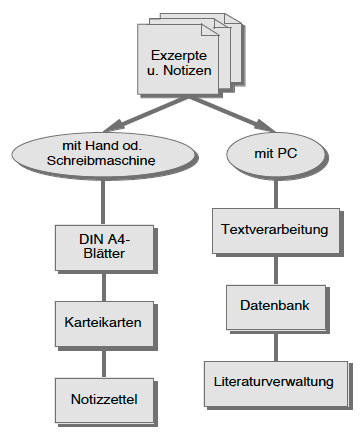
\includegraphics{images/lesen-notizen-min} 

}

\caption{Exzerpieren und notieren}\label{fig:unnamed-chunk-19}
\end{figure}

Wenn man von Hand exzerpieren will, sollte man sich von vornherein auf
ein bestimmtes System festlegen und dabei bleiben:

\begin{itemize}
\tightlist
\item
  DIN A4-Blätter bieten genügend Platz auch für längere Exzerpte. Mit
  Papier sollte man dabei nicht sparen, also: breiten Rand lassen für
  nachträgliche Stichworte und Zusätze; auch Seitenzahlen werden am
  besten am Rand vermerkt. Auch für kurze Exzerpte eigene Blätter
  verwenden; am Kopf die Quelle und die Schlagwörter vermerken.
  A4-Blätter lassen sich gut in Ordnern ablegen, zusammen mit den evt.
  gemachten auszugsweisen Kopien. Listen von Fundstellen werden nach
  Schlagwörtern bzw. Fragestellungen geführt.
\item
  Karteikarten für Exzerpte sollten nicht zu klein sein -- das verleitet
  zum Zerstückeln, bei dem leicht der Zusammenhang verloren geht. DIN
  A6-Format (Postkartengröße) ist für längere Exzerpte
  (Zusammenfassungen, Kommentare) eigentlich schon zu klein. Die Ablage
  im Karteikasten erfolgt alphabetisch nach Autor oder -- wenn man ein
  klares Schema hat -- nach Schlagwörtern. Vorteil bei Karteikarten ist
  die Möglichkeit, sie nach verschiedenen Gesichtspunkten zu ordnen und
  sie zur Übersicht aufzubreiten.
\item
  Notizzettel: Für sie gilt dasselbe wie für Karteikarten. Sie werden
  vor allem zum Einlegen in Bücher verwendet und können mit Karteikarten
  und großen Blättern kombiniert werden.
\end{itemize}

Ganz gleich welches System Sie verwenden: Exzerpte sollten so
geschrieben sein, dass sie auch nach ein paar Wochen oder Monaten noch
lesbar und verständlich sind und das mühsame, wenn nicht gar unmögliche
erneute Nachlesen im bearbeiteten Buch ersparen.

Allen Methoden des computergestützten Exzerpierens ist gemeinsam, dass
ein einmal erfasster Text im Prinzip immer wieder verwendbar ist. Unter
diesem Gesichtspunkt zahlt es sich auch aus, handschriftliche Exzerpte
(z. B. aus der Bibliothek mitgebrachte) nochmals einzugeben. Die Methode
will aber doch gut überlegt und geplant werden. Vor allem müssen Sie
gleich zu Beginn entscheiden, welche Anwendungssoftware Sie für Ihre
Notizen verwenden: das Textverarbeitungsprogramm, eine Datenbank oder
die Literaturverwaltungssoftware.

Exzerpte mit einem Textverarbeitungsprogramm zu schreiben ist dann
sinnvoll, wenn es sich dabei um längere, zusammenhängende Texte handelt.
Das Anlegen von vielen Einzeldateien (etwa entsprechend Karteikarten)
führt zu Problemen in der Dateibenennung und -verwaltung. Die
Suchfunktion von Textverarbeitungsprogrammen erlaubt es, in Dateien nach
beliebigen Ausdrücken zu suchen. Damit kann jede Stelle in einem Exzerpt
relativ leicht wiedergefunden werden. Ein weiterer Vorteil kann sein,
dass Stücke (Zitate) aus Exzerpten leicht von einer Datei zur anderen
übertragen werden können. Selbst wenn man die Arbeit mit dem selben
Programm wie die Exzerpte schreibt, sollte man beim Exzerpieren auf alle
Formatierungen verzichten, weil dadurch die Übernahme von Textstücken
nur mühsamer wird.

Literaturverwaltungsprogramme bieten meistens die Möglichkeit zur
Eingabe auch längerer Texte zu jedem Datensatz (= bibliografische
Angabe). Das ist ausreichend, um zu jedem Werk genau ein Exzerpt
(Zusammenfassung, Abstract) zu erfassen. Es ist nicht geeignet, um ein
Buch zu „verzetteln``, also nach Schlagworten, Themen usw. getrennte
Exzerpte und Notizen anzulegen.

Dem altbewährten Karteikasten in der Funktion am nächsten kommen
Datenbankverwaltungen. Das Entwickeln und Benutzen einer
maßgeschneiderten Exzerptdatenbank erfordert bei modernen Programmen
keine besonderen Computerkenntnisse. Wenn auch längere Exzerpte erfasst
werden sollen, ist ein Programm erforderlich, das entsprechend große
Textfelder zulässt. Ein Datensatz (= Karteikarte) so einer Datenbank
könnte Felder vorsehen für:

\begin{itemize}
\tightlist
\item
  Quellenangabe: eindeutiger Kurzbeleg (z. B. in Harvard-Notation). Die
  vollständige Literaturangabe ist hier nicht notwendig und würde nur
  unnötigen Aufwand beim Eingeben bedeuten. Die bibliografischen Angaben
  sind für jedes Werk vollständig in einer anderen Datenbank oder in der
  Literaturverwaltung erfasst.
\item
  Seitenangabe (von -- bis): bei kurzen Exzerpten (z. B. wörtlichen
  Zitaten) steht hier die genaue Seitenangabe. Bei längeren Exzerpten
  muss zusätzlich im Text jeweils die genaue Angabe erfolgen
  (Seitenwechsel markieren, z. B. mit „/``).
\item
  Schlagwortliste: Sie muss nicht von vornherein festgelegt werden --
  was meistens sowieso nicht möglich ist, wenn man sich in ein Thema
  erst einarbeitet. Andererseits kommt man aber in Probleme, wenn man
  mit dem Erfinden neuer Schlagworte zu großzügig und eilig ist -- sie
  verlieren dann ihren Wert, nämlich die Exzerpte zu gruppieren und zu
  inhaltlichen Gesichtspunkten zusammenzubringen. Die Eingabe mehrerer
  Schlagworte in ein Feld ist nur sinnvoll, wenn das Programm das
  gesamte Feld nach einem Ausdruck durchsuchen kann und nicht nur den
  Anfang.
\item
  Text: Obwohl Datenbanksoftware meistens Formatierungsmöglichkeiten
  (wie Fett, Kursiv, Schriftgrößen etc.) bieten, wird man sich so weit
  wie möglich auf Rohtext beschränken. Die spätere Übernahme in die
  Arbeit lässt sich durch Kopieren und Einfügen (Copy and Paste)
  bewerkstelligen. Dieses Feld für den „Inhalt`` kann lange Exzerpte
  ebenso aufnehmen wie den bloßen Hinweis auf eine Fundstelle.
\end{itemize}

Eine Datenbank hat den Vorteil, dass sie nach verschiedenen
Gesichtspunkten geordnet, durchsucht und gefiltert werden kann. Es
können also alle Exzerpte zu einem bestimmten Buch ebenso
zusammengesucht werden wie alle Einträge zu einem bestimmten Schlagwort.

Es ist Geschmacksache, ob man lieber am Bildschirm Exzerpte durchliest
oder sie ausdruckt und auch auf Papier aufbewahrt. Lesen ist auf Papier
weniger anstrengend und gibt oft einen besseren Überblick. Außerdem kann
man in den ausgedruckten Exzerpten nach Belieben anstreichen und
hervorheben, was man beim gespeicherten Text ja vermieden hat.
Zusammenfassend stellen wir die beiden Methoden des „Aneignens`` von
Texten - Kopieren und Exzerpieren - einander gegenüber.

\begin{longtable}[]{@{}lllll@{}}
\caption{\textbf{\label{tab:kopieren-exzerpieren} Kopieren oder
Exzerpieren?}}\tabularnewline
\toprule
\begin{minipage}[b]{0.28\columnwidth}\raggedright\strut
\strut
\end{minipage} & \begin{minipage}[b]{0.04\columnwidth}\raggedright\strut
+/-\strut
\end{minipage} & \begin{minipage}[b]{0.21\columnwidth}\raggedright\strut
Kopien\strut
\end{minipage} & \begin{minipage}[b]{0.04\columnwidth}\raggedright\strut
+/-\strut
\end{minipage} & \begin{minipage}[b]{0.28\columnwidth}\raggedright\strut
Exzerpte\strut
\end{minipage}\tabularnewline
\midrule
\endfirsthead
\toprule
\begin{minipage}[b]{0.28\columnwidth}\raggedright\strut
\strut
\end{minipage} & \begin{minipage}[b]{0.04\columnwidth}\raggedright\strut
+/-\strut
\end{minipage} & \begin{minipage}[b]{0.21\columnwidth}\raggedright\strut
Kopien\strut
\end{minipage} & \begin{minipage}[b]{0.04\columnwidth}\raggedright\strut
+/-\strut
\end{minipage} & \begin{minipage}[b]{0.28\columnwidth}\raggedright\strut
Exzerpte\strut
\end{minipage}\tabularnewline
\midrule
\endhead
\begin{minipage}[t]{0.28\columnwidth}\raggedright\strut
Zugriff auf Originaltext\strut
\end{minipage} & \begin{minipage}[t]{0.04\columnwidth}\raggedright\strut
\textbf{+}\strut
\end{minipage} & \begin{minipage}[t]{0.21\columnwidth}\raggedright\strut
jederzeit möglich\strut
\end{minipage} & \begin{minipage}[t]{0.04\columnwidth}\raggedright\strut
\textbf{-}\strut
\end{minipage} & \begin{minipage}[t]{0.28\columnwidth}\raggedright\strut
nicht oder nur mit großem Aufwand möglich \vspace{5mm}\strut
\end{minipage}\tabularnewline
\begin{minipage}[t]{0.28\columnwidth}\raggedright\strut
Zeitaufwand\strut
\end{minipage} & \begin{minipage}[t]{0.04\columnwidth}\raggedright\strut
\textbf{+}\strut
\end{minipage} & \begin{minipage}[t]{0.21\columnwidth}\raggedright\strut
gering\strut
\end{minipage} & \begin{minipage}[t]{0.04\columnwidth}\raggedright\strut
\textbf{-}\strut
\end{minipage} & \begin{minipage}[t]{0.28\columnwidth}\raggedright\strut
hoch \vspace{5mm}\strut
\end{minipage}\tabularnewline
\begin{minipage}[t]{0.28\columnwidth}\raggedright\strut
Kosten\strut
\end{minipage} & \begin{minipage}[t]{0.04\columnwidth}\raggedright\strut
\textbf{-}\strut
\end{minipage} & \begin{minipage}[t]{0.21\columnwidth}\raggedright\strut
bei zahlreichen Kopien berücksichtigen\strut
\end{minipage} & \begin{minipage}[t]{0.04\columnwidth}\raggedright\strut
\textbf{+}\strut
\end{minipage} & \begin{minipage}[t]{0.28\columnwidth}\raggedright\strut
praktisch keine \vspace{5mm}\strut
\end{minipage}\tabularnewline
\begin{minipage}[t]{0.28\columnwidth}\raggedright\strut
Aufbewahrung\strut
\end{minipage} & \begin{minipage}[t]{0.04\columnwidth}\raggedright\strut
\strut
\end{minipage} & \begin{minipage}[t]{0.21\columnwidth}\raggedright\strut
Ordner, umfangreiche Kopien heften od. binden -\textgreater{} Schachteln
\vspace{5mm}\strut
\end{minipage} & \begin{minipage}[t]{0.04\columnwidth}\raggedright\strut
\strut
\end{minipage} & \begin{minipage}[t]{0.28\columnwidth}\raggedright\strut
Dateien -\textgreater{} Datensicherung, Ausdrucke -\textgreater{} Ordner
\vspace{5mm}\strut
\end{minipage}\tabularnewline
\begin{minipage}[t]{0.28\columnwidth}\raggedright\strut
Bearbeitung\strut
\end{minipage} & \begin{minipage}[t]{0.04\columnwidth}\raggedright\strut
\textbf{-}\strut
\end{minipage} & \begin{minipage}[t]{0.21\columnwidth}\raggedright\strut
muss erst noch erfolgen\strut
\end{minipage} & \begin{minipage}[t]{0.04\columnwidth}\raggedright\strut
\textbf{+}\strut
\end{minipage} & \begin{minipage}[t]{0.28\columnwidth}\raggedright\strut
Exzerpieren ist bereits Bearbeitung \vspace{5mm}\strut
\end{minipage}\tabularnewline
\begin{minipage}[t]{0.28\columnwidth}\raggedright\strut
Gefahr\strut
\end{minipage} & \begin{minipage}[t]{0.04\columnwidth}\raggedright\strut
\textbf{-}\strut
\end{minipage} & \begin{minipage}[t]{0.21\columnwidth}\raggedright\strut
blindes Sammeln, zu viel wörtliches Zitieren\strut
\end{minipage} & \begin{minipage}[t]{0.04\columnwidth}\raggedright\strut
\textbf{-}\strut
\end{minipage} & \begin{minipage}[t]{0.28\columnwidth}\raggedright\strut
unvollständige Exzerpte (z. B. neu auftretende Gesichtspunkte);
„Verzettelung`` = Verlust des Zusammenhangs \vspace{5mm}\strut
\end{minipage}\tabularnewline
\begin{minipage}[t]{0.28\columnwidth}\raggedright\strut
Vorteil\strut
\end{minipage} & \begin{minipage}[t]{0.04\columnwidth}\raggedright\strut
\textbf{+}\strut
\end{minipage} & \begin{minipage}[t]{0.21\columnwidth}\raggedright\strut
Besitz des Originals (Zitate, Markieren); schriftl. Ausarbeitung evt.
direkt in Formulierungsphase \vspace{5mm}\strut
\end{minipage} & \begin{minipage}[t]{0.04\columnwidth}\raggedright\strut
\textbf{+}\strut
\end{minipage} & \begin{minipage}[t]{0.28\columnwidth}\raggedright\strut
gründliche Aneignung; Textteile evt. f. Arbeit direkt verwendbar
(Dateien!) \vspace{5mm}\strut
\end{minipage}\tabularnewline
\bottomrule
\end{longtable}

Um es kurz zu sagen: „Kopieren oder Exzerpieren`` ist keine
Grundsatzfrage, sondern beides kann sehr gut kombiniert werden, wenn man
die Vor- und Nachteile kennt. Der „Besitz`` der Texte in Form von
Kopien, Ausdrucken oder Büchern macht das wörtliche Abschreiben
überflüssig, und man kann sich beim (zusätzlichen) Exzerpieren auf die
Verarbeitung (Zusammenfassung, Paraphrase, Kritik \ldots{})
konzentrieren. Exzerpieren wiederum fördert die intensive und kritische
Auseinandersetzung mit dem Text.

\section{Aufgabe: Lesen}\label{aufgabe-lesen}

\begin{longtable}[]{@{}l@{}}
\caption{\textbf{\label{tab:aufgabe5-test} Übungsaufgabe}}\tabularnewline
\toprule
\begin{minipage}[t]{0.97\columnwidth}\raggedright\strut
Verfassen Sie eine praphrasierende Notiz zu den folgenden
Textausschnitten. Trennen Sie eigene Gedanken und Anmerkungen deutlich
von denen des Autors. Lesen Sie dazu jeden Text aufmerksam durch und
legen ihn dann weg, während Sie Ihre Notiz schreiben.
\vspace{-6mm}\strut
\end{minipage}\tabularnewline
\begin{minipage}[t]{0.97\columnwidth}\raggedright\strut
\textbf{(A)} Langzeituntersuchungen zur Frage des Einflusses einer
frühkindlichen Heranführung an naturwissenschaftliche Themenfelder
liegen bislang keine vor, was insbesondere auf zwei Gründe
zurückzuführen ist: Zum einen sind sie enorm kostenaufwendig, zum
anderen sehr zeitintensiv, muss doch mit einem Untersuchungszeitraum von
mindestens zehn Jahren gerechnet werden.

Allenfalls über indirekte Methoden lässt sich eine Langzeitwirkung
frühkindlicher Erfahrugen erschließen, nämlich durch Interpretation
biographischer Daten. Ausgewertet wurden insgesamt 1345 biographische
Daten von Studienanfängern. Erhoben wurde dieses Datenmaterial im Rahmen
der Vergabe eines Stipendiums an Abiturienten, die sich für einen
Chemie-Diplomstudiengang entschieden und aufgefordert wurden, ihrem
Bewerbungsmaterial eine persönliche Begründung beizufügen, aus welchem
Grund sie einen Chemie Diplomstudiengang aufnehmen möchten.

Die Auswertung der persönlichen Begleitschreiben in Hinblick auf
außerschulische und schulische Einflüsse sowie den Beginn der
Interessenbildung nach Schulstufen gibt Abb. 2 wieder: Es zeigt sich,
dass die Vorschule mit 22 \% das zweitgrößte Segment bildet. Die
Grundschule ist dagegen kaum vertreten. Da der Einführungsunterricht der
Fächer Physik und Chemie in die Sekundarstufe I fällt, lassen sich in
diesem Zeitraum die meisten Nennungen für die Interessenbildung und
Motivation zum Chemiestudium finden. Die Sekundarstufe II spielt dagegen
eine eher untergeordnete Rolle. Demnach haben bei 37 \% der Bewerber
außerschulische Einflüsse zum Chemiestudium bewogen, davon mit großem
Abstand vorschulische Impulse.

(aus: Lück, Gisela: Naturwissenschaften im frühen Kindesalter - Zur
Vertiefung von Sachinteresse zwischen Verschulung und Spielerei. In:
Frühe Bildungsprozesse und Schulische Anschlussfähigkeit. Hrsg. von Toni
Hansel. Centaurus Verlag, Herbolzheim (2004), S.118-135.)
\vspace{-6mm}\strut
\end{minipage}\tabularnewline
\begin{minipage}[t]{0.97\columnwidth}\raggedright\strut
\textbf{(B)} \ldots{} Ich möchte nicht verschweigen, dass ich
hinsichtlich solcher Reformvorschläge {[}bzgl. Erzieherinnenausbildung
an Fachhochschulen bzw. Universitäten{]} eher pessimistisch eingestellt
bin. Fachhoschulen sind nicht für eine besonders praxisnahe Ausbildung
von Sozialpädagog/innen „berühmt``, und die Lehrerausbildung an
Universitäten wird seit vielen Jahren stark kritisiert. So dürfte eine
Verlagerung der Erzieherausbildung an Fachhochschulen oder Universitäten
wohl kaum zu einer besseren Berufsausbildung führen. Hinzu kommt, dass
derzeit weder an Fachhochschulen noch an Universitäten mehr als 10 bis
15 im Bereich der Frühpädagogik qualifizierte Professor/innen und
Assistent/innen zur Verfügung stehen. \ldots{}

Vor allem aber beruht mein Pessimismus auf folgenden Gründen: akademisch
ausgebildete Erzieher/innen haben Anspruch auf ein viel höheres Gehalt.
Und ich sehe nicht die geringste Bereitschaft bei Kommunen, Ländern und
Wohlfahrtsverbänden, hierfür die finanziellen Mittel aufzubringen. Und
was soll mit den derzeit berufstätigen Erzieher/innen passieren? Sollen
sie in mehrjährigen Fortbildungsgängen nachqualifiziert werden? Auf den
Stand von Fachhochschul- oder Universitätsabsolvent/innen gebracht
werden? Und was soll mit den Fachschulen passieren? Sollen sie aufgelöst
und die dort tätigen Lehrkräfte in die Arbeitslosigkeit entlassen
werden?

(aus: Textor, Martin R.: Erziehr/innenausbildung: zwischen
Akademisierung und Elementarisierung. Online-Handbuch
Kindergartenpädagogik,
\url{http://www.kindergartenpaedagogik.de/})\strut
\end{minipage}\tabularnewline
\bottomrule
\end{longtable}

\chapter{Schreiben}\label{schreiben}

\begin{figure}

{\centering 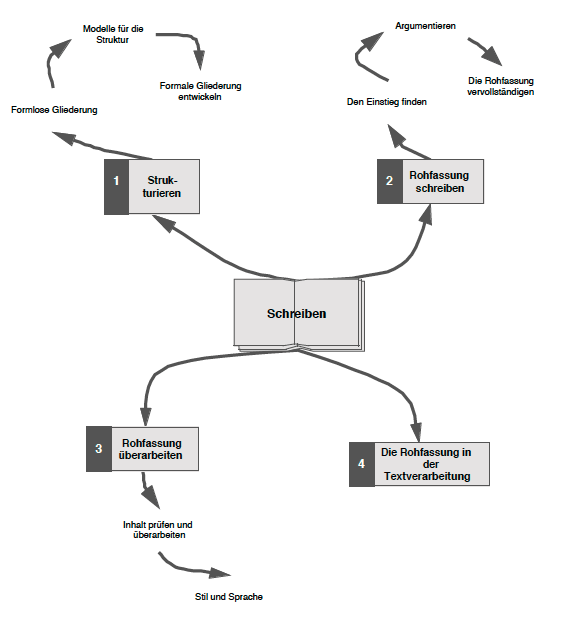
\includegraphics{images/schreiben-min} 

}

\caption{Schreiben (Überblick)}\label{fig:unnamed-chunk-20}
\end{figure}

Das Material ist gesammelt, gelesen und ausgewertet. Wahrscheinlich gibt
es nun bereits jede Menge Notizen, Dateien und Zettel mit Fragen,
Gedanken und Hinweisen. Nun geht es darum, das Ergebnis dieser Arbeit
niederzuschreiben. Wir behandeln in diesem Kapitel den Weg vom Material
zur fertigen Niederschrift in vier großen Schritten:

\begin{figure}

{\centering 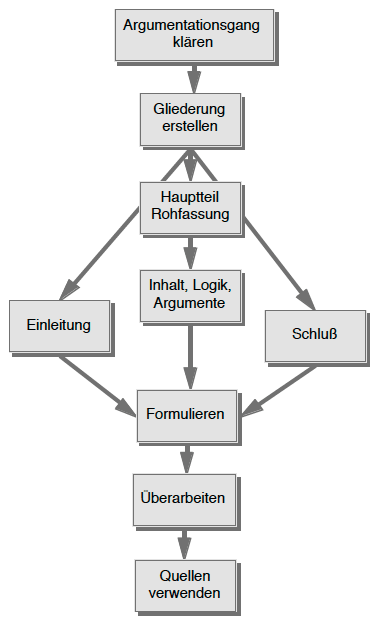
\includegraphics{images/schreiben-argumentationsgang-min} 

}

\caption{Prozess des Schreibens}\label{fig:unnamed-chunk-21}
\end{figure}

\begin{itemize}
\tightlist
\item
  Strukturieren (Gliederung)
\item
  Inhalte niederschreiben (Rohfassung)
\item
  Inhalt überarbeiten (Überarbeitung)
\item
  Glätten und Fertigstellen (Sprache, Stil)
\end{itemize}

Ihre Aufgabe ist es, Ihre Gedanken zusammenhängend, nachvollziehbar und
verständlich zu Papier zu bringen. Dieses Kapitel beschäftigt sich
sozusagen mit der inneren Form der Arbeit, die „äußere Form`` -- also
das Erfüllen formaler Anforderungen und die ansprechende Gestaltung --
möchten wir davon trennen und später behandeln (siehe Kapitel
„Fertigstellen der Arbeit``). Der Prozess des Schreibens ist in der
nebenstehenden Grafik grob dargestellt.

Eine Einschränkung möchten wir aber noch vorausschicken: Das Verfahren,
das wir hier beschreiben, führt von „oben`` (dem Gesamtthema, der
Grobstruktur) nach „unten`` (zur Feinstruktur, zu den einzelnen
Abschnitten und Absätzen). Dieses „Top- Down``-Vorgehen hat sich zwar
oft bewährt, vor allem, weil es den Überblick und Zusammenhang bewahren
hilft, aber es passt nicht jedem und nicht immer: Manche können besser
schreiben, wenn sie einen Teil (fast) fertig ausformulieren und den Rest
rundherum bauen; andere haben vielleicht eine gesamte Arbeit wie eine
Geschichte bereits im Kopf und können sie von Anfang bis Ende
niederschreiben. Wir glauben zwar, dass es gerade für wenig geübte
Schreiber besser ist, von einer Gliederung weg zu arbeiten, aber
letztlich muss jede(r) selbst herausfinden, welche Methode am besten
funktioniert.

\section{Strukturieren}\label{strukturieren}

Im ersten Schritt des Top-Down-Verfahrens wird die Gliederung
festgelegt, also die logische Abfolge der einzelnen Teile, Argumente,
Fälle usw.

\subsection{Formlose Gliederung}\label{formlose-gliederung}

Stellen Sie sich die Gliederung der Arbeit besser nicht als
vorweggenommenes Inhaltsverzeichnis vor, sondern als eine strukturierte
Zusammenfassung. Die Titel und Überschriften, die wir meistens
verwenden, sind zu kurz und zu wenig aussagekräftig, um als Anleitung
für das Schreiben herhalten zu können. Um nicht in diese Gewohnheit zu
verfallen, ist es oft besser, ganz andere Methoden zu verwenden, um eine
Struktur zu schaffen, z. B. ein Mind-Map (siehe „Thematik erschließen,
„öffnen```` auf Seite 15) zu zeichnen oder die Gliederung ganz formlos
zu erzählen.

Der Einstieg ins Schreiben und Formulieren wird sehr erleichtert, wenn
man die Gliederung in ganzen Sätzen und Fragen formuliert. Man beginnt
mit dem Thema oder Arbeitstitel und verwandelt ihn in die Leitfrage, um
die sich die gesamte Arbeit dreht. Das ist oft gar nicht leicht. Die
Mühe lohnt sich, denn diese Formulierung ist vielleicht ein erster
Prüfstein dafür, ob Sie Ihr Thema wirklich bewältigt haben: Hinter den
Formulierungsschwierigkeiten können sich inhaltliche Unklarheiten und
Ungereimtheiten verstecken, die sich beim detaillierten Ausarbeiten als
Stolpersteine erweisen können. Die Arbeit an der Fragestellung und der
Grobstruktur wird deshalb ja auch schon sehr früh, vor der
Materialsammlung und -bearbeitung, begonnen.

Dann beschreiben Sie in möglichst einfachen Sätzen den Gedankengang der
Arbeit. Diese Beschreibung kann noch ganz grob und kurz sein, sodass
vielleicht ein ganzes Kapitel mit einem einzigen Satz zusammengefasst
wird. Diese „Geschichte`` bekommt niemand zu lesen -- sie braucht daher
gar nicht wissenschaftlich zu klingen. Alltagssprache ist dafür
geeigneter, weil wir uns darin direkter und auch emotional ausdrücken
können. Einfachen Sätzen sehen wir sofort an, ob sie logisch aufeinander
aufbauen, und damit können wir den Aufbau der Arbeit gleich auf seine
Folgerichtigkeit prüfen. Dazu ein Beispiel:

\begin{longtable}[]{@{}ll@{}}
\caption{\textbf{\label{tab:gliederung} Vom alltagssprachlichen Erzählen zur
Gliederung}}\tabularnewline
\toprule
\begin{minipage}[b]{0.51\columnwidth}\raggedright\strut
Sie erzählen \ldots{}\strut
\end{minipage} & \begin{minipage}[b]{0.43\columnwidth}\raggedright\strut
In der Gliederung wird darauf \ldots{}\strut
\end{minipage}\tabularnewline
\midrule
\endfirsthead
\toprule
\begin{minipage}[b]{0.51\columnwidth}\raggedright\strut
Sie erzählen \ldots{}\strut
\end{minipage} & \begin{minipage}[b]{0.43\columnwidth}\raggedright\strut
In der Gliederung wird darauf \ldots{}\strut
\end{minipage}\tabularnewline
\midrule
\endhead
\begin{minipage}[t]{0.51\columnwidth}\raggedright\strut
Autor A behauptet, dass X\strut
\end{minipage} & \begin{minipage}[t]{0.43\columnwidth}\raggedright\strut
Wiedergabe der These und \vspace{-6mm}\strut
\end{minipage}\tabularnewline
\begin{minipage}[t]{0.51\columnwidth}\raggedright\strut
Er meint damit, dass \ldots{}\strut
\end{minipage} & \begin{minipage}[t]{0.43\columnwidth}\raggedright\strut
Analyse\vspace{-6mm}\strut
\end{minipage}\tabularnewline
\begin{minipage}[t]{0.51\columnwidth}\raggedright\strut
Das hat mich immer schon gestört.\strut
\end{minipage} & \begin{minipage}[t]{0.43\columnwidth}\raggedright\strut
Widerspruch \vspace{-6mm}\strut
\end{minipage}\tabularnewline
\begin{minipage}[t]{0.51\columnwidth}\raggedright\strut
Es würde nämlich bedeuten, dass \ldots{}\strut
\end{minipage} & \begin{minipage}[t]{0.43\columnwidth}\raggedright\strut
Motivation des Widerspruchs: Konsequenz von X \vspace{-6mm}\strut
\end{minipage}\tabularnewline
\begin{minipage}[t]{0.51\columnwidth}\raggedright\strut
\ldots{} und das hätte zur Folge, dass \ldots{}\strut
\end{minipage} & \begin{minipage}[t]{0.43\columnwidth}\raggedright\strut
negative Auswirkung\vspace{-6mm}\strut
\end{minipage}\tabularnewline
\begin{minipage}[t]{0.51\columnwidth}\raggedright\strut
Deshalb will ich zeigen, dass er unrecht hat\strut
\end{minipage} & \begin{minipage}[t]{0.43\columnwidth}\raggedright\strut
Hypothese\vspace{-6mm}\strut
\end{minipage}\tabularnewline
\begin{minipage}[t]{0.51\columnwidth}\raggedright\strut
Ich verwende dazu\strut
\end{minipage} & \begin{minipage}[t]{0.43\columnwidth}\raggedright\strut
\vspace{-6mm}\strut
\end{minipage}\tabularnewline
\begin{minipage}[t]{0.51\columnwidth}\raggedright\strut
Fall 1, mit dem sich die Autoren B und C beschäftigt haben, und\strut
\end{minipage} & \begin{minipage}[t]{0.43\columnwidth}\raggedright\strut
Argument 1 und Belege\vspace{-6mm}\strut
\end{minipage}\tabularnewline
\begin{minipage}[t]{0.51\columnwidth}\raggedright\strut
Fall 2, mit dem sich die Autoren D und E beschäftigt haben\strut
\end{minipage} & \begin{minipage}[t]{0.43\columnwidth}\raggedright\strut
Argument 2 und Belege\vspace{-6mm}\strut
\end{minipage}\tabularnewline
\begin{minipage}[t]{0.51\columnwidth}\raggedright\strut
Fall 1 und Fall 2 zeigen, dass Autor A unrecht hat.\strut
\end{minipage} & \begin{minipage}[t]{0.43\columnwidth}\raggedright\strut
Zusammenfassung, Schlussfolgerung und Ergebnis\vspace{-6mm}\strut
\end{minipage}\tabularnewline
\begin{minipage}[t]{0.51\columnwidth}\raggedright\strut
Da tauchen natürlich neue Fragen auf:\strut
\end{minipage} & \begin{minipage}[t]{0.43\columnwidth}\raggedright\strut
Fragen, die das Ergebnis aufwirft\vspace{-6mm}\strut
\end{minipage}\tabularnewline
\begin{minipage}[t]{0.51\columnwidth}\raggedright\strut
Wieso irrt sich ein Autor wie A bei sowas? (Da will ich aber höchstens
ganz kurz darauf eingehen)\strut
\end{minipage} & \begin{minipage}[t]{0.43\columnwidth}\raggedright\strut
Frage 1: Hintergrund der These (wird nicht näher
behandelt)\vspace{-6mm}\strut
\end{minipage}\tabularnewline
\begin{minipage}[t]{0.51\columnwidth}\raggedright\strut
Wackelt seine ganze Theorie, weil er sich bei X irrt?\strut
\end{minipage} & \begin{minipage}[t]{0.43\columnwidth}\raggedright\strut
Frage 2: logische Konsequenzen des Irrtums \vspace{-6mm}\strut
\end{minipage}\tabularnewline
\begin{minipage}[t]{0.51\columnwidth}\raggedright\strut
Das kann ich in einem Fall nachweisen\strut
\end{minipage} & \begin{minipage}[t]{0.43\columnwidth}\raggedright\strut
exemplarischer Nachweis \vspace{-6mm}\strut
\end{minipage}\tabularnewline
\begin{minipage}[t]{0.51\columnwidth}\raggedright\strut
Die Konsequenzen des Irrtums müsste man auch im Rest seines Werks
untersuchen\strut
\end{minipage} & \begin{minipage}[t]{0.43\columnwidth}\raggedright\strut
Schluss: Anregung für weitere wissenschaftliche Arbeit\strut
\end{minipage}\tabularnewline
\bottomrule
\end{longtable}

\section{Modelle für die Struktur}\label{modelle-fur-die-struktur}

Wenn Sie wissenschaftliche Literatur lesen, werden Sie bemerken, dass es
nicht tausend verschiedene Arten gibt, einen Text zu strukturieren.
Meistens folgt der Aufbau des gesamten Textes und/oder seiner Teile
einem der folgenden Modelle:

\begin{longtable}[]{@{}lll@{}}
\caption{\textbf{\label{tab:gliederung2} Modell für die Gliederung
wählen}}\tabularnewline
\toprule
\begin{minipage}[b]{0.14\columnwidth}\raggedright\strut
Sie machen \ldots{}\strut
\end{minipage} & \begin{minipage}[b]{0.36\columnwidth}\raggedright\strut
Das bedeutet\strut
\end{minipage} & \begin{minipage}[b]{0.41\columnwidth}\raggedright\strut
Beispiel\strut
\end{minipage}\tabularnewline
\midrule
\endfirsthead
\toprule
\begin{minipage}[b]{0.14\columnwidth}\raggedright\strut
Sie machen \ldots{}\strut
\end{minipage} & \begin{minipage}[b]{0.36\columnwidth}\raggedright\strut
Das bedeutet\strut
\end{minipage} & \begin{minipage}[b]{0.41\columnwidth}\raggedright\strut
Beispiel\strut
\end{minipage}\tabularnewline
\midrule
\endhead
\begin{minipage}[t]{0.14\columnwidth}\raggedright\strut
eine Beschreibung\strut
\end{minipage} & \begin{minipage}[t]{0.36\columnwidth}\raggedright\strut
Das Ganze wird in Teile zerlegt, die einzeln beschrieben (analysiert)
werden. Am Ende kann sich daraus eine Gesamtbeschreibung oder -sicht
ergeben.\strut
\end{minipage} & \begin{minipage}[t]{0.41\columnwidth}\raggedright\strut
Thema ist z. B. das Entstehen von Gruppen. Dazu nehmen Sie als
teilnehmende Beobachterin an einer Gruppenreise teil. Die ausführliche
Darstellung Ihrer Beobachtungen folgt diesem Modell, z. B. in Form eines
Reisetagebuchs \vspace{-6mm}\strut
\end{minipage}\tabularnewline
\begin{minipage}[t]{0.14\columnwidth}\raggedright\strut
eine Klassifizierung\strut
\end{minipage} & \begin{minipage}[t]{0.36\columnwidth}\raggedright\strut
Ein Ding wird einer Gruppe oder Klasse zugeordnet. Dazu müssen zuerst
die Merkmale der Gruppe dargestellt werden. Dann wird gezeigt, dass das
fragliche Ding diese Merkmale aufweist und daher zur Gruppe
gehört.\strut
\end{minipage} & \begin{minipage}[t]{0.41\columnwidth}\raggedright\strut
Sie müssen zeigen, dass aus der zufälligen Ansammlung von Teilnehmern
der Reisegruppe zu Beginn der Reise eine „Gruppe`` im wissenschaftlichen
Sinn wird. Sie erläutern daher, was eine Gruppe ausmacht, und zeigen
dann, dass diese Merkmale auf die Reisegruppe zutreffen
\vspace{-6mm}\strut
\end{minipage}\tabularnewline
\begin{minipage}[t]{0.14\columnwidth}\raggedright\strut
einen Vergleich\strut
\end{minipage} & \begin{minipage}[t]{0.36\columnwidth}\raggedright\strut
kann als eine Sonderform der Klassifizierung gesehen werden. Um zwei
Dinge vergleichen zu können, müssen sie Gemeinsamkeiten haben, d. h. zu
einer Gruppe gehören -- sie werden beide klassifiziert. Erst dann kann
man über Unterschiede reden.\strut
\end{minipage} & \begin{minipage}[t]{0.41\columnwidth}\raggedright\strut
Sie können die Reisegruppe mit anderen Formen von Gruppen vergleichen,
z. B. einem Projektteam, einer Schulklasse oder einem
Brieftaubenzüchterclub. Auch für die „Vergleichsgruppe`` müssen Sie
zuerst zeigen, dass es sich um eine Gruppe in Ihrem Sinn handelt.
\vspace{-6mm}\strut
\end{minipage}\tabularnewline
\begin{minipage}[t]{0.14\columnwidth}\raggedright\strut
eine Bewertung (Evaluation)\strut
\end{minipage} & \begin{minipage}[t]{0.36\columnwidth}\raggedright\strut
Um einen Gegenstand bewerten zu können, muss man einerseits seine
Merkmale einzeln betrachten und für diese Merkmale (Kriterien) einen
Maßstab oder Standard haben, an dem man sie messen kann.\strut
\end{minipage} & \begin{minipage}[t]{0.41\columnwidth}\raggedright\strut
Wenn Sie z. B. die Konfliktfähigkeit Ihrer Reisegruppe bewerten wollen,
brauchen Sie a) Merkmale, an denen sich die Konfliktfähigkeit zeigt und
b) einen Maßstab (z. B. aus der Literatur) mit der Sie diese Kriterien
einstufen können \vspace{-6mm}\strut
\end{minipage}\tabularnewline
\begin{minipage}[t]{0.14\columnwidth}\raggedright\strut
eine Chronik\strut
\end{minipage} & \begin{minipage}[t]{0.36\columnwidth}\raggedright\strut
Historische Prozesse, Abläufe, Verfahren, Projekte haben einen
Zeitverlauf, an dem sich die Darstellung orientieren kann. Es gibt
Anfang und Ende (oder Zwischenstand) und dazwischen Phasen, Schritte,
Epochen usw. Am Ende kann die gegenwärtige Situation stehen oder auch
ein Blick in die Zukunft.\strut
\end{minipage} & \begin{minipage}[t]{0.41\columnwidth}\raggedright\strut
Wenn Sie in einem Teil Ihrer Arbeit den Verlauf der Gruppenreise
berichten, so bietet sich dafür dieses Modell an. \vspace{-6mm}\strut
\end{minipage}\tabularnewline
\begin{minipage}[t]{0.14\columnwidth}\raggedright\strut
einen Problemlösungsvorschlag\strut
\end{minipage} & \begin{minipage}[t]{0.36\columnwidth}\raggedright\strut
Etwas muss zuerst als Problem wahrgenommen werden, bevor man es lösen
kann. Man wird zeigen, warum es nicht oder nicht befriedigend gelöst
wurde, bevor man eigene Vorschläge dazu macht.\strut
\end{minipage} & \begin{minipage}[t]{0.41\columnwidth}\raggedright\strut
Sie zeigen z. B. das Problem auf, dass bisherige Untersuchungen von
Gruppenverhalten sich auf existierende Gruppen beschränkten, und dass
dadurch relevante Aspekte unbeachtet blieben. Anhand der Untersuchung
der Reisegruppe zeigen Sie die Besonderheiten in entstehenden Gruppen
auf.\strut
\end{minipage}\tabularnewline
\bottomrule
\end{longtable}

Viele Themen bieten von sich aus einen Aufbau an, der wie „natürlich``
aus ihnen zu folgen scheint. Die Aufgliederung eines Ganzen in einzelne
Teile, Aspekte, Merkmale usw. kann sich so beinahe von selbst ergeben
oder sich an der im Fach üblichen Reihenfolge orientieren. So werden in
den technischen und naturwissenschaftlichen Disziplinen fast alle
Artikel nach dem Modell „Problemlösungsvoschlag`` geschrieben: Es wird
eine (noch) ungelöste Frage aufgezeigt und anschließend der eigene
Lösungsvorschlag präsentiert und diskutiert.

\subsection{Formale Gliederung
entwickeln}\label{formale-gliederung-entwickeln}

Die frei geschriebene Struktur der Arbeit wird nun in eine provisorische
Gliederung umgewandelt: Die einzelnen Sätze und Gedanken bilden darin
Abschnitte und Kapitel. Diese Gliederung braucht nur so weit
ausgearbeitet und verfeinert zu werden, dass sie einen Arbeitsbehelf für
den Beginn des Schreibens darstellt. Sie kann sich im Lauf der Arbeit
noch deutlich und mehrmals ändern, sodass es überflüssig oder sogar
hinderlich ist, sie schon zu Beginn bis in alle Einzelheiten und bis zum
letzten Argument auszuarbeiten.

\begin{longtable}[]{@{}l@{}}
\caption{\textbf{\label{tab:strukturieren} Strukturieren}}\tabularnewline
\toprule
\begin{minipage}[t]{0.97\columnwidth}\raggedright\strut
\begin{itemize}
\tightlist
\item
  Wie kann der Aufbau in Form eines frei geschriebenen,
  zusammenhängenden Textes dargestellt werden? \vspace{-6mm} \textbar{}
  +----------------------------------------------------------------------------------------------------------------------------------+
\item
  Welche informelle Gliederung ergibt sich aus der Zerlegung dieses
  Textes in einzelne Fragen und Aussagen? \vspace{-6mm}
\end{itemize}\strut
\end{minipage}\tabularnewline
\begin{minipage}[t]{0.97\columnwidth}\raggedright\strut
\begin{itemize}
\tightlist
\item
  Welches Modell steht hinter der Struktur? Passt das Modell zum Thema
  und zur Zielsetzung? \vspace{-6mm}
\end{itemize}\strut
\end{minipage}\tabularnewline
\begin{minipage}[t]{0.97\columnwidth}\raggedright\strut
\begin{itemize}
\tightlist
\item
  Welche provisorische formale Gliederung ergibt sich aus der
  informellen Struktur? \vspace{-6mm}
\end{itemize}\strut
\end{minipage}\tabularnewline
\begin{minipage}[t]{0.97\columnwidth}\raggedright\strut
\begin{itemize}
\tightlist
\item
  Wie kann die Gliederung so weit verfeinert werden, dass sie als
  Leitfaden für das Schreiben brauchbar ist? \vspace{-6mm}
\end{itemize}\strut
\end{minipage}\tabularnewline
\bottomrule
\end{longtable}

\section{Rohfassung schreiben}\label{rohfassung-schreiben}

\subsection{Den Einstieg finden}\label{den-einstieg-finden}

Das eigentliche Niederschreiben einer wissenschaftlichen Arbeit bereitet
vielen Leuten Probleme, die bis zur totalen Schreibhemmung`` führen
können. Man glaubt, alles schon im Kopf zu haben, aber sobald man es zu
Papier bringen will, ist jeder klare Gedanke fort, man weiß nicht, wo
man anfangen soll, die Sätze drücken nicht das aus, was man sagen
möchte, oder sie wirken banal, sobald man sie Schwarz auf Weiß sieht,
und so weiter.

Hilfen dafür, wie diese Schwierigkeiten überwunden werden können, finden
sich in diesem Buch schon in den vorangegangenen Kapiteln: Wenn man
bereits beim Konzipieren und Lesen immer wieder mit eigenen Notizen und
Entwürfen das Schreiben zum Thema übt, wird die Schwelle zur
Niederschrift niedriger. Darüber hinaus gibt es Trainings und
Anleitungen, mit denen man das schriftliche Formulieren üben und
Schreibhemmungen überwinden kann.

Schreiben ist nicht nur das Festhalten und Aufzeichnen von fertigen
Gedankengängen, sondern selbst eine Entwicklungsarbeit. Viele Gedanken
und Argumente entwickeln sich erst beim Schreiben, aber ebenso zeigen
sich dabei Brüche oder Widersprüche, die vorher noch nicht aufgefallen
sind. Schreiben hat also gleichzeitig zwei Ziele: sich selbst Klarheit
zu verschaffen und dem (zukünftigen) Leser etwas mitzuteilen.

Vor allem beim Schreiben einer ersten Rohfassung können diese Ziele
leicht miteinander in Konflikt geraten und das Schreiben behindern. Es
ist schon schwer genug, einen Gedankengang schlüssig von Anfang bis Ende
zu entwickeln und schriftlich niederzulegen. Manche Schreiber, die sich
dazu auch noch vornehmen, gleichzeitig stilistisch gut, verständlich und
überzeugend -- also für den Leser -- zu schreiben, überfordern sich
damit selber. Die beiden Ziele -- Denken und Kommunizieren -- lassen
sich zwar nicht ganz trennen. Aber wenn man merkt, dass man ein Argument
zwar bereits im Kopf hat, aber noch nicht schön und treffend formulieren
kann, ist es besser, es fürs erste eben bloß so zu formulieren, wie es
gerade geht, als es wegen der Sorge um die sprachliche Gestaltung
womöglich wieder entgleiten zu lassen.

Gerade bei Qualifikationsarbeiten sehen Studierende im Geiste die
Prüferin als die (einzige) Leserin vor sich und versuchen, ihren
Ansprüchen gerecht zu werden: Das Schreiben wird zur ständigen
Prüfungssituation, in der sie die Kritik und die Benotung schon
vorwegnehmen und oft strenger sind als die Prüferin. Unter dieser
scharfen Kontrolle fällt das Formulieren natürlich doppelt schwer.
Stellen Sie sich besser als Leserin eine andere Person vor, z. B. Ihre
StudienkollegInnen, die zwar insgesamt eine ähnliche fachliche Kompetenz
haben wie Sie, sich aber in Ihrem speziellen Thema weit weniger
auskennen. Das kann Ihnen einen Anhaltspunkt dafür liefern, wie
kompliziert oder einfach Sie schreiben müssen, was Sie voraussetzen
können und was Sie erklären müssen.

Oft ist es gerade der Anfang -- der erste Satz, die erste Seite -- der
am meisten Schwierigkeiten bereitet. Bei vielen verursacht die leere
Seite (oder der leere Bildschirm) Hemmungen und Blockaden. Man will den
Anfang „richtig`` erwischen: Er soll sozusagen als Visitenkarte der
ganzen Arbeit den Leser interessieren und beeindrucken. Diese Ansprüche
sind aber für das Schreiben der Rohfassung viel zu hoch. Wenn sich die
Einleitung nicht schon von selbst anbietet, kann man sich mit Tricks
über die erste Schwelle hinwegschwindeln, um ins Schreiben
hineinzukommen. Ein solcher Trick ist z. B. das „freie Schreiben``: Man
schreibt wieder ganz unwissenschaftlich und nur für sich selbst auf, was
einem zum Anfang einfällt und was man später darin haben möchte, und
setzt dann dort fort, wo man eben mit dem richtigen Formulieren und
Argumentieren beginnen kann.

Sich gleich um eine richtige Einleitung zu bemühen, kann unnötiger
Aufwand sein: Eine Einleitung soll ja einen Ausblick auf und Überblick
über die Arbeit geben. Die Arbeit kann sich aber beim und durch das
Schreiben doch noch anders entwickeln, als man anfangs denkt, und dann
passt die Einleitung sowieso nicht mehr. Es ist also besser, diesen Teil
erst zum Schluss zu schreiben. Für den Anfang genügt gerade so viel, wie
man braucht, um den Einstieg zu finden und „in Fahrt`` zu kommen.

Dagegen wird der Hauptteil so vollständig und durchgängig wie möglich
geschrieben. Das betrifft wiederum in dieser Phase in erster Linie die
Inhalte: die verarbeitete Literatur, die Analysen, Argumente, Belege,
Beispiele usw. Das Schreiben der Rohfassung ist der Zeitpunkt, zu dem
man diese Stücke zusammenhängt und in eine einheitliche Struktur bringt.
Sackgassen, Brüche und Widersprüche sind Anzeichen für lückenhafte oder
unlogische Argumentationsgänge -- wenn man sich in der Rohfassung über
sie hinwegschwindelt und „Löcher`` im Text stehen lässt, verschiebt man
die Arbeit daran bloß auf später oder verrennt sich -- schwerwiegender
-- in eine falsche Richtung, die nicht mehr zu ändern ist.

Dabei ist dieselbe Vorgangsweise wie bei der Einleitung günstig: Das
heißt, man schreibt die Rohfassung möglichst in einem Fluss, ganz gleich
in welcher Sprache und welchem Stil. Wo Formulierungsprobleme drohen,
den Schreibprozess ins Stocken zu bringen, behilft man sich eben mit
vorläufigen „lockeren`` und frei geschriebenen Passagen und Übergängen.

Für die Abfolge der Teile und Argumente gibt es klassische Muster, die
man je nach Themenstellung, Zielsetzung und Material wählen wird. Ihr
Zweck ist es, der Leserin (und den eigenen Gedanken) einen Leitfaden zu
liefern und die Arbeit als eine Einheit erkennen zu lassen.

\begin{longtable}[]{@{}lll@{}}
\caption{\textbf{\label{tab:argumente} Aufbau von
Argumenten}}\tabularnewline
\toprule
\begin{minipage}[b]{0.19\columnwidth}\raggedright\strut
Sie verwenden das Muster\ldots{}\strut
\end{minipage} & \begin{minipage}[b]{0.39\columnwidth}\raggedright\strut
\ldots{} und gehen dabeo so vor\strut
\end{minipage} & \begin{minipage}[b]{0.33\columnwidth}\raggedright\strut
Hinweis\strut
\end{minipage}\tabularnewline
\midrule
\endfirsthead
\toprule
\begin{minipage}[b]{0.19\columnwidth}\raggedright\strut
Sie verwenden das Muster\ldots{}\strut
\end{minipage} & \begin{minipage}[b]{0.39\columnwidth}\raggedright\strut
\ldots{} und gehen dabeo so vor\strut
\end{minipage} & \begin{minipage}[b]{0.33\columnwidth}\raggedright\strut
Hinweis\strut
\end{minipage}\tabularnewline
\midrule
\endhead
\begin{minipage}[t]{0.19\columnwidth}\raggedright\strut
Vom Ganzen zum Teil\strut
\end{minipage} & \begin{minipage}[t]{0.39\columnwidth}\raggedright\strut
Problemstellung allgemein, dann einzelne Fragen, Aspekte, Merkmale;
oder: zuerst Behauptung, dann Beleg oder Beispiel\strut
\end{minipage} & \begin{minipage}[t]{0.33\columnwidth}\raggedright\strut
fördert Überblick; die Einzelteile müssen relevant sein, sonst
erscheinen sie der Leserin überflüssig („alles schon gesagt``)
\vspace{-6mm}\strut
\end{minipage}\tabularnewline
\begin{minipage}[t]{0.19\columnwidth}\raggedright\strut
Vom Teil zum Ganzen\strut
\end{minipage} & \begin{minipage}[t]{0.39\columnwidth}\raggedright\strut
umgekehrt: einzelne Aspekte, daraus verallgemeinern; ein Beispiel oder
Fall, daraus allgemeine(re) Aussage entwikkeln\strut
\end{minipage} & \begin{minipage}[t]{0.33\columnwidth}\raggedright\strut
wirkt schlüssig und logisch; der Überblick beim Schreiben und Lesen ist
schwieriger zu wahren \vspace{-6mm}\strut
\end{minipage}\tabularnewline
\begin{minipage}[t]{0.19\columnwidth}\raggedright\strut
Spannung\strut
\end{minipage} & \begin{minipage}[t]{0.39\columnwidth}\raggedright\strut
vom weniger Wichtigen, Spektakulären etc. zum Neuen, Zentralen;
Widersprüche, Gegensätze stehenlassen und erst zum Schluss
auflösen\strut
\end{minipage} & \begin{minipage}[t]{0.33\columnwidth}\raggedright\strut
weckt Neugier beim Leser, wenn zielgerichtet auf den Höhepunkt hin
geschrieben wird. \vspace{-6mm}\strut
\end{minipage}\tabularnewline
\begin{minipage}[t]{0.19\columnwidth}\raggedright\strut
Zunehmende Komplexität\strut
\end{minipage} & \begin{minipage}[t]{0.39\columnwidth}\raggedright\strut
vom Einfachsten, Einleuchtendsten zum Schwierigeren, Fraglicheren\strut
\end{minipage} & \begin{minipage}[t]{0.33\columnwidth}\raggedright\strut
notwendige Vorgangsweise, wenn beim Leser schrittweise Vorverständnis
und Vorkenntnisse aufgebaut werden müssen\strut
\end{minipage}\tabularnewline
\bottomrule
\end{longtable}

Nicht nur der Text als Ganzes, sondern auch jeder seiner Teile sollten
idealerweise eine klare, folgerichtige Struktur aufweisen. Das heißt,
dass man bei jedem Kapitel, Abschnitt, ja sogar Absatz wieder so vorgeht
wie bei der Gliederung der gesamten Arbeit: Man sagt oder besser notiert
sich dafür jeweils in einem Satz, worum es geht: Wo steht man im
Gedankengang am Anfang, wo will man am Ende sein? Welcher Schritt wird
im gerade bearbeiteten Teil gemacht? Wie hängt er mit der gesamten
Arbeit zusammen?

\section{Argumentieren}\label{argumentieren}

Bei „Argumentieren`` denkt man zuerst an das mündliche Streitgespräch
und die Diskussion. Die Spielregeln des Argumentierens gelten aber auch
für schriftliche Arbeiten, denn diese sind ja (zumindest gedanklich)
„zeitverzögerte`` Debatten. Ihre „Diskussionspartner`` sind einerseits
die AutorInnen, mit deren Werken Sie sich auseinandersetzen,
andererseits die zukünftigen LeserInnen, die Sie überzeugen und mit
denen Sie ins Gespräch kommen möchten.

Die Regeln des Argumentierens sorgen erst dafür, dass Aussagen überhaupt
vernünftig diskutiert werden können. Wir können hier nur kurz die
wichtigsten Grundsätze kurz erläutern (mehr dazu in YYY Kienpointner
1996):

\begin{longtable}[]{@{}lll@{}}
\caption{\textbf{\label{tab:argumente2} Richtig
argumentieren}}\tabularnewline
\toprule
\begin{minipage}[b]{0.19\columnwidth}\raggedright\strut
Sie sollten \ldots{}\strut
\end{minipage} & \begin{minipage}[b]{0.39\columnwidth}\raggedright\strut
Das bedeutet \ldots{}\strut
\end{minipage} & \begin{minipage}[b]{0.33\columnwidth}\raggedright\strut
schlechtes Beispiel\strut
\end{minipage}\tabularnewline
\midrule
\endfirsthead
\toprule
\begin{minipage}[b]{0.19\columnwidth}\raggedright\strut
Sie sollten \ldots{}\strut
\end{minipage} & \begin{minipage}[b]{0.39\columnwidth}\raggedright\strut
Das bedeutet \ldots{}\strut
\end{minipage} & \begin{minipage}[b]{0.33\columnwidth}\raggedright\strut
schlechtes Beispiel\strut
\end{minipage}\tabularnewline
\midrule
\endhead
\begin{minipage}[t]{0.19\columnwidth}\raggedright\strut
sachlich argumentieren\strut
\end{minipage} & \begin{minipage}[t]{0.39\columnwidth}\raggedright\strut
Kritik, Begründungen usw. müssen sich direkt auf den Inhalt einer
Aussage beziehen\strut
\end{minipage} & \begin{minipage}[t]{0.33\columnwidth}\raggedright\strut
Das inhaltlich richtige Argument eines Autors wird deswegen abgelehnt,
weil er als frauenfeindlich gilt \vspace{-6mm}\strut
\end{minipage}\tabularnewline
\begin{minipage}[t]{0.19\columnwidth}\raggedright\strut
jede Behauptung begründen\strut
\end{minipage} & \begin{minipage}[t]{0.39\columnwidth}\raggedright\strut
Durch Belege, Beweise etc. zeigen, wie Sie zu Ihrer Behauptung gekommen
sind\strut
\end{minipage} & \begin{minipage}[t]{0.33\columnwidth}\raggedright\strut
Sie kommentieren ein Zitat etwa mit „Das ist ganz offensichtlich
falsch.`` ohne zu sagen, warum es (Ihrer Meinung nach) falsch ist.
\vspace{-6mm}\strut
\end{minipage}\tabularnewline
\begin{minipage}[t]{0.19\columnwidth}\raggedright\strut
andere Meinungen gelten lassen\strut
\end{minipage} & \begin{minipage}[t]{0.39\columnwidth}\raggedright\strut
andere AutorInnen richtig und im Kontext darstellen und sie erst dann
kritisieren\strut
\end{minipage} & \begin{minipage}[t]{0.33\columnwidth}\raggedright\strut
Durch unzusammenhängende und verzerrende Darstellung wird einem Autor
etwas unterstellt, was er nie behauptet hat. \vspace{-6mm}\strut
\end{minipage}\tabularnewline
\begin{minipage}[t]{0.19\columnwidth}\raggedright\strut
ausreichend explizit sein\strut
\end{minipage} & \begin{minipage}[t]{0.39\columnwidth}\raggedright\strut
Einzelschritte der Argumentation so darstellen, dass die LeserInnen sie
nachvollziehen können\strut
\end{minipage} & \begin{minipage}[t]{0.33\columnwidth}\raggedright\strut
„Der Schnee ist weiß. Daher gehe ich morgen Schifahren`` mag für Sie
selbst ganz logisch sein, weil Sie die einzelnen Schritte kennen, die
vom einen zum anderen führen. Diese Schritte kennt aber sonst niemand.
\vspace{-6mm}\strut
\end{minipage}\tabularnewline
\begin{minipage}[t]{0.19\columnwidth}\raggedright\strut
nicht unnötig explizit sein\strut
\end{minipage} & \begin{minipage}[t]{0.39\columnwidth}\raggedright\strut
Gemeinsame implizite Voraussetzungen müssen und können nicht alle
explizit gemacht werden\strut
\end{minipage} & \begin{minipage}[t]{0.33\columnwidth}\raggedright\strut
Jeden kleinsten Gedankenschritt darzustellen, kann unnötig und ermüdend
sein. Ebenso können Sie in einer Definition nicht jeden verwendeten
Begriff definieren. \vspace{-6mm}\strut
\end{minipage}\tabularnewline
\begin{minipage}[t]{0.19\columnwidth}\raggedright\strut
plausible Argumentationsmuster verwenden\strut
\end{minipage} & \begin{minipage}[t]{0.39\columnwidth}\raggedright\strut
Muster wie Definition, Zuordnung, Vergleich, Ursache-Wirkung usw.
korrekt verwenden\strut
\end{minipage} & \begin{minipage}[t]{0.33\columnwidth}\raggedright\strut
zirkuläre Definition wie z. B. „Eine Irrlehre ist ein Glaube, der die
Menschen in die Irre führt`` \vspace{-6mm}\strut
\end{minipage}\tabularnewline
\begin{minipage}[t]{0.19\columnwidth}\raggedright\strut
logisch argumentieren\strut
\end{minipage} & \begin{minipage}[t]{0.39\columnwidth}\raggedright\strut
aus Prämissen korrekte Schlüsse ziehen\strut
\end{minipage} & \begin{minipage}[t]{0.33\columnwidth}\raggedright\strut
unzulässige Schlussfolgerung wie z. B. „Regenwürmer sind Tiere.
Regenwürmer haben keine Beine. Also haben Tiere keine Beine.``
\vspace{-6mm}\strut
\end{minipage}\tabularnewline
\bottomrule
\end{longtable}

Diese Regeln klingen -- so allgemein ausgedrückt -- beinahe trivial.
Beim wissenschaftlichen Schreiben erfährt man, dass es gar nicht so
einfach ist, sie zu erfüllen. Nach unserer Erfahrung scheint es
Studierenden besonders schwerzufallen, den angemessenen Mittelweg
zwischen einem Zuviel und einem Zuwenig an Explizitheit zu finden. Die
Auswüchse sowohl in die eine wie in die andere Richtung zeigen aber
nicht bloß die persönlichen Neigungen verschiedener AutorInnen -- sie
können auch in ein und derselben Arbeit auftreten.

Gegen die Faustregel „nicht unnötig explizit sein`` wird vorzugsweise
ganz am Beginn der Arbeit verstoßen, u.zw. dort, wo die in der Arbeit
verwendeten Begriffe definiert werden. Jede Definition verwendet
wiederum Begriffe, die man glaubt, nun ebenfalls definieren zu müssen.
Die Forderung, dass jeder Begriff definiert sein soll, ist nicht
erfüllbar, denn dann kommt man nie ans Ende des Definierens und zum
Beginn der eigentlichen Arbeit. Wo sollte man also die Grenze ziehen?

Die Begriffe, die für Ihr Thema von zentraler Bedeutung sind, sollten
allerdings definiert werden, um von vornherein bei den LeserInnen eine
einheitliche Ausgangsbasis für Ihre Argumentation zu schaffen.

Wenn Sie zu diesen Begriffen mehrere, voneinander abweichende oder sogar
einander widersprechende Definitionen finden, so können Sie z. B. die
wichtigsten Vertreter darstellen und diskutieren, um anschließend (immer
mit Begründung)

\begin{itemize}
\tightlist
\item
  eine der präsentierten Definitionen zu übernehmen
\item
  zwei oder mehrere der Definitionen zu „Ihrer`` (weiteren, genaueren
  \ldots{}) Definition zu kombinieren
\item
  die vorhandenen Definitionen zurückzuweisen und Ihre eigene zu finden.
\end{itemize}

Häufig wird man mit den vorgefundenen Definitionen nicht zufrieden sein
und versuchen, es selbst besser und für die Arbeit passender zu machen.
Das ist jedoch gar nicht einfach, da ja eine „richtige`` Definition
genau alles treffen sollte, was zur Kategorie gehört, und genau all das
ausschließen, was nicht dazu gehört. Statt nun ewig an einer Definition
zu feilen, die schon mit Merkmalen vollgestopft und doch nicht
ausreichend präzis ist, ist es durchaus legitim, sich auf eine
„Arbeitsdefinition`` zu beschränken, für die man nur begrenzte
Gültigkeit beansprucht, also z. B. „In dieser Arbeit werde ich daher X
vereinfacht definieren als \ldots{}.``.

Natürlich darf diese Definition nicht völlig dem widersprechen, was der
Begriff im Wissenschafts- oder Alltagsverständnis bedeutet. Außerdem
muss die Definition „operational`` sein, d. h. sie muss nachvollziehbar
und damit überprüfbar sein. „Als X bezeichne ich alle jene Fälle, die
ich in dieser Arbeit behandle, aber keine anderen`` ist zum Beispiel
nicht nachvollziehbar, denn Sie erklären nicht, wodurch sich Ihre Fälle
von allen anderen unterscheiden.

Der Fehler, zu wenig explizit zu sein, unterläuft einem dagegen eher
später im Lauf der Arbeit und des Schreibens: vielleicht hat man einen
Gedankengang während der Vorarbeiten schon so oft verfolgt, dass er
einem bereits selbstverständlich erscheint, und schreibt nur noch das
Ergebnis hin. Für den außenstehenden Leser ist das zu wenig, es
erscheint unbegründet und sprunghaft. Dagegen hilft, wenn man den
eigenen Text mit den Augen des Lesers zu sehen versucht, und wenn man
ihn tatsächlich von anderen durchlesen lässt.

\subsection{Die Rohfassung
vervollständigen}\label{die-rohfassung-vervollstandigen}

Die Literatur, die im Text verarbeitet wird, ist in der Rohfassung
bereits mit Zitaten und Quellenangaben eingebaut. Wie man beim Schreiben
mit der Literatur umgeht, wird im folgenden Kapitel (siehe Kapitel
„Zitieren``) beschrieben.

Um den Faden beim Schreiben der Rohfassung nicht zu verlieren, haben Sie
im ersten Anlauf vielleicht Kapitelanfänge ausgelassen und Teile ohne
Übergang aneinandergereiht. Diese Lücken sollten bereits in der
Rohfassung zumindest versuchsweise geschlossen werden. Unter „Übergang``
ist hier ein Absatz (oder mehrere) gemeint, die einen Teil abschließen
und gleichzeitig den nächsten ankündigen. Für den Schreiber muss daraus
ebenso wie für den Leser klar werden, was bis dorthin erreicht wurde und
warum das Folgende die notwendige und logische Fortsetzung davon ist.
Wenn man Schwierigkeiten mit diesen Übergängen hat, die nicht bloß mit
dem Ausformulieren zu tun haben, dann kann das ein ernstzunehmendes
Warnsignal dafür sein, dass das eigentliche Problem im Aufbau der Arbeit
liegt: Wenn dem Aufbau ein logischer Gedankengang zugrunde liegt, dann
lässt sich dieser auch sprachlich formulieren -- vielleicht holprig,
aber doch. Wenn die Formulierung so gar nicht kommen will, könnte das
Problem auch daran liegen, dass der Aufbau eben nicht folgerichtig ist.

Meistens wird der Schluss einer Arbeit, der eine Zusammenfassung,
Ergebnisse oder einen Ausblick bringt -- ähnlich wie die Einleitung in
der Rohfassung -- nur provisorisch geschrieben werden können: Bei
längeren Texten hat man nach der intensiven Arbeit an der Formulierung
der einzelnen Argumente oft am Ende nicht mehr jenen Blick für das
Ganze, der für einen guten Abschluss notwendig wäre. Dann ist es besser,
die endgültige Formulierung des Schlusses erst nach dem Durchlesen und
Überarbeiten vorzunehmen.

\begin{longtable}[]{@{}l@{}}
\caption{\textbf{\label{tab:rohfassung} Rohfassung
schreiben}}\tabularnewline
\toprule
\begin{minipage}[t]{0.97\columnwidth}\raggedright\strut
\begin{itemize}
\tightlist
\item
  Wird der Grundsatz „Inhalt geht vor Form`` beachtet? (Stil, Sprache,
  Layout in dieser Phase nicht zu sehr beachten) \vspace{-6mm}
  \textbar{}
  +----------------------------------------------------------------------------------------------------------------------------------+
\item
  Wird -- bei Schreibschwierigkeiten -- der Einstieg provisorisch und
  alltagssprachlich überbrückt? \vspace{-6mm}
\end{itemize}\strut
\end{minipage}\tabularnewline
\begin{minipage}[t]{0.97\columnwidth}\raggedright\strut
\begin{itemize}
\tightlist
\item
  Sind alle Inhalte formuliert und Lücken im Argumentationsgang
  geschlossen? \vspace{-6mm}
\end{itemize}\strut
\end{minipage}\tabularnewline
\begin{minipage}[t]{0.97\columnwidth}\raggedright\strut
\begin{itemize}
\tightlist
\item
  Ist der Hauptteil vollständig schriftlich formuliert? (bei
  Schreibschwierigkeiten vorläufige, lockere Formulierungen verwenden)
  \vspace{-6mm}
\end{itemize}\strut
\end{minipage}\tabularnewline
\begin{minipage}[t]{0.97\columnwidth}\raggedright\strut
\begin{itemize}
\tightlist
\item
  Wurden die Quellen bereits mit Belegen zitiert? \vspace{-6mm}
\end{itemize}\strut
\end{minipage}\tabularnewline
\begin{minipage}[t]{0.97\columnwidth}\raggedright\strut
\begin{itemize}
\tightlist
\item
  Sind die Übergänge zumindest provisorisch formuliert? \vspace{-6mm}
\end{itemize}\strut
\end{minipage}\tabularnewline
\begin{minipage}[t]{0.97\columnwidth}\raggedright\strut
\begin{itemize}
\tightlist
\item
  Gibt es bereits einen -- wenn auch evt. provisorischen -- Schluss?
\end{itemize}\strut
\end{minipage}\tabularnewline
\bottomrule
\end{longtable}

\section{Rohfassung überarbeiten}\label{rohfassung-uberarbeiten}

Beim Überarbeiten der Rohfassung geht es darum,

\begin{itemize}
\tightlist
\item
  eine gründliche inhaltliche Prüfung durchzuführen
\item
  Argumentationsgang und Zusammenhang zu kontrollieren
\item
  provisorische Formulierungen in endgültige umzuwandeln
\item
  Zitate und Quellenangaben auf Korrektheit und Vollständigkeit zu
  prüfen
\item
  Sprache und Stil zu verbessern und zu vereinheitlichen
\end{itemize}

Das Überarbeiten der Rohfassung ist genauso wichtig wie das erste
Niederschreiben -- und kann auch genauso lang (oder sogar länger)
dauern. Bei der Zeitplanung muss man berücksichtigen, dass es mit dem
einmaligen Schreiben der Arbeit noch nicht getan ist. Der Grund dafür
ist, dass beim ersten Schreiben viele Gedankengänge und Argumente erst
entwickelt werden und die Arbeit dabei zum ersten Mal komplett
„durchdacht`` wird. Der Anspruch, bei diesem ersten Durchdenken auch
schon einwandfrei logisch, klar, verständlich und vielleicht auch noch
stilistisch gut zu schreiben, wäre einfach zu hoch: Deswegen ist ein
zweiter Durchgang notwendig.

\subsection{Inhalt prüfen und
überarbeiten}\label{inhalt-prufen-und-uberarbeiten}

Idealerweise hat man genug Zeit, um die Rohfassung ein paar Tage liegen
zulassen und sich mit ganz anderen Dingen zu beschäftigen. Das erzeugt
die notwendige Distanz, um sie dann besser aus der Sicht einer Leserin
beurteilen zu können.

Die Fragen, die man beim Durchlesen an den Text stellt, sind ganz
ähnlich wie die des „analytischen Lesers`` (siehe „Analytisches Lesen``,
S. 99), mit einem großen Unterschied: Hier handelt es sich nicht um
einen fertigen, fremden Text, sondern um den eigenen, vorläufigen, der
sich noch in alle Richtungen verändern und verbessern lässt.

\begin{longtable}[]{@{}l@{}}
\caption{\textbf{\label{tab:rohfassung2} Inhaltliche Fragen an die
Rohfassung}}\tabularnewline
\toprule
\begin{minipage}[t]{0.97\columnwidth}\raggedright\strut
\begin{itemize}
\tightlist
\item
  Wird die Fragestellung, das Thema deutlich? Wird der Leserin die
  Bedeutung der Fragestellung klargemacht? \vspace{-6mm} \textbar{}
  +----------------------------------------------------------------------------------------------------------------------------------+
\item
  Welche Erwartungen werden im Leser geweckt -- und werden sie auch
  erfüllt? \vspace{-6mm}
\end{itemize}\strut
\end{minipage}\tabularnewline
\begin{minipage}[t]{0.97\columnwidth}\raggedright\strut
\begin{itemize}
\tightlist
\item
  Hat die gesamte Arbeit einen Bezug zum Thema, und wird dieser Bezug
  überall deutlich hergestellt? \vspace{-6mm}
\end{itemize}\strut
\end{minipage}\tabularnewline
\begin{minipage}[t]{0.97\columnwidth}\raggedright\strut
\begin{itemize}
\tightlist
\item
  Ist der Aufbau des Ganzen, der Kapitel, der Absätze sinnvoll und
  nachvollziehbar? Bildet die Arbeit ein sinnvolles Ganzes?
  \vspace{-6mm}
\end{itemize}\strut
\end{minipage}\tabularnewline
\begin{minipage}[t]{0.97\columnwidth}\raggedright\strut
\begin{itemize}
\tightlist
\item
  Sind die einzelnen Argumente inhaltlich und logisch richtig und
  ausreichend ausgeführt und belegt, sodass sie für die Leser
  nachvollziehbar und einleuchtend sind? \vspace{-6mm}
\end{itemize}\strut
\end{minipage}\tabularnewline
\begin{minipage}[t]{0.97\columnwidth}\raggedright\strut
\begin{itemize}
\tightlist
\item
  Nach Ende der Überarbeitung: Sind alle Teile (Einleitung, Schluss,
  Übergänge, provisorisch angedeutete Passagen usw.) fertig
  ausformuliert und überarbeitet?
\end{itemize}\strut
\end{minipage}\tabularnewline
\bottomrule
\end{longtable}

Die Arbeit, die notwendig ist, um Schwächen in diesen Aspekten
auszubessern, wird sich kaum auf kleine Korrekturen und Umformulierungen
beschränken können. Manchmal ist es notwendig, ganze Teile neu zu
schreiben. Davor darf man keine allzu große Scheu haben: manchmal ist es
sogar einfacher, Passagen wegzuwerfen und sie unbelastet vom bereits
einmal Geschriebenen neu zu formulieren, statt zu versuchen, schwache
Abschnitte durch kosmetische Operationen an einzelnen Wendungen und
Sätzen zu retten. Selbst wenn die Zeit für die Überarbeitung nicht durch
die äußeren Umstände begrenzt ist, muss man sich ein festes Ziel setzen,
um zu einem Ende zu kommen. Sicher könnte man den Text immer wieder
überarbeiten und weiter verbessern, aber das ist nicht der Sinn der
Sache. Viele Schreibende sind ihren eigenen Texten gegenüber zu kritisch
und finden sie nie wirklich gut. Da hilft es, sich einen typischen
Leser(kreis) vorzustellen, sich den Zweck der Arbeit in Erinnerung zu
rufen und nicht ganz allgemein zu fragen, ob die Arbeit „gut`` ist,
sondern ob sie genau für diese Leser und diesen Zweck „gut genug`` ist.
\#\#\# Stil und Sprache

Obwohl man schon beim Überarbeiten der Inhalte durch das Bemühen um
Klarheit und Verständlichkeit viele Verbesserungen an Ausdruck und
Sprache vorgenommen hat, ist auch noch ein eigener Durchgang von
Vorteil, bei dem man nur mehr auf den Stil und die Sprache der Arbeit
achtet. Damit ist aber noch nicht das Korrekturlesen gemeint, bei dem
nur noch Fehler ausgebessert werden. Hier geht es vorerst noch um
grundlegendere Fragen wie

\begin{itemize}
\tightlist
\item
  Wie spricht man in einer wissenschaftlichen Arbeit von sich selbst?
\item
  Wie redet man Leser an?
\item
  Wie hält man es mit den geschlechtsneutralen Formen?
\item
  Wie lang sollen Sätze sein?
\item
  Wie variiert man im Ausdruck?
\end{itemize}

Wir können hier nur ganz wenige der häufigsten Probleme und notwendigen
Entscheidungen aufzeigen.

\begin{longtable}[]{@{}lll@{}}
\caption{\textbf{\label{tab:stil} Stil in wissenschaftlichen
Arbeiten}}\tabularnewline
\toprule
\begin{minipage}[b]{0.11\columnwidth}\raggedright\strut
Sie wollen \ldots{}\strut
\end{minipage} & \begin{minipage}[b]{0.42\columnwidth}\raggedright\strut
Sie verwenden \ldots{}\strut
\end{minipage} & \begin{minipage}[b]{0.39\columnwidth}\raggedright\strut
Sie vermeiden \ldots{}\strut
\end{minipage}\tabularnewline
\midrule
\endfirsthead
\toprule
\begin{minipage}[b]{0.11\columnwidth}\raggedright\strut
Sie wollen \ldots{}\strut
\end{minipage} & \begin{minipage}[b]{0.42\columnwidth}\raggedright\strut
Sie verwenden \ldots{}\strut
\end{minipage} & \begin{minipage}[b]{0.39\columnwidth}\raggedright\strut
Sie vermeiden \ldots{}\strut
\end{minipage}\tabularnewline
\midrule
\endhead
\begin{minipage}[t]{0.11\columnwidth}\raggedright\strut
von sich selbst schreiben\strut
\end{minipage} & \begin{minipage}[t]{0.42\columnwidth}\raggedright\strut
„ich``, wenn es sich um Ihre eigene Arbeit, Untersuchung usw. handelt;
unpersönliche Formulierungen, um die (relative) Allgemeingültigkeit
Ihrer Aussagen zu unterstreichen \vspace{-6mm}\strut
\end{minipage} & \begin{minipage}[t]{0.39\columnwidth}\raggedright\strut
das veraltete „wir`` (außer natürlich bei einer Arbeit mit mehreren
Autoren); Passivformen ohne Akteur („es wird gezeigt``, „ \ldots{}
werden dargestellt`` usw.) \vspace{-6mm}\strut
\end{minipage}\tabularnewline
\begin{minipage}[t]{0.11\columnwidth}\raggedright\strut
geschlechtsneutral schreiben\strut
\end{minipage} & \begin{minipage}[t]{0.42\columnwidth}\raggedright\strut
Das sog. Binnen-I (StudentInnen), männliche und weibliche Form
(Studenten und Studentinnen), Schrägstriche (Student/ inn/en),
geschlechtsneutrale Formen (Studierende) oder -- radikal -- nur die
weibliche Form (Studentinnen)\strut
\end{minipage} & \begin{minipage}[t]{0.39\columnwidth}\raggedright\strut
unbegründete Vermischung verschiedener Strategien; ausschließlich
männliche Formen ohne jede Begründung; langatmige und die Lesbarkeit
erschwerende Formen \vspace{-6mm}\strut
\end{minipage}\tabularnewline
\begin{minipage}[t]{0.11\columnwidth}\raggedright\strut
Leser und Leserinnen ansprechen\strut
\end{minipage} & \begin{minipage}[t]{0.42\columnwidth}\raggedright\strut
„der Leser`` und „die Leserin`` bzw. geschlechtsneutrale Formen\strut
\end{minipage} & \begin{minipage}[t]{0.39\columnwidth}\raggedright\strut
„Sie`` oder „du``, außer in handlungsanleitenden Texten
\vspace{-6mm}\strut
\end{minipage}\tabularnewline
\begin{minipage}[t]{0.11\columnwidth}\raggedright\strut
sich klar und kurz ausdrücken\strut
\end{minipage} & \begin{minipage}[t]{0.42\columnwidth}\raggedright\strut
aussagekräftige Verben, aktive Konstruktionen, Subjekte mit Inhalt\strut
\end{minipage} & \begin{minipage}[t]{0.39\columnwidth}\raggedright\strut
passive und unpersönliche Kosntruktionen wie „es wird zu zeigen sein,
dass'', Hauptwortstil wie „die Annahme einer Zunahme der Beteiligung
\ldots{}`` \vspace{-6mm}\strut
\end{minipage}\tabularnewline
\begin{minipage}[t]{0.11\columnwidth}\raggedright\strut
kurze, prägnante Sätze schreiben\strut
\end{minipage} & \begin{minipage}[t]{0.42\columnwidth}\raggedright\strut
mehrere kürzere Sätze\strut
\end{minipage} & \begin{minipage}[t]{0.39\columnwidth}\raggedright\strut
überlange, komplizierte und verschachtelte Satzkonstruktionen
\vspace{-6mm}\strut
\end{minipage}\tabularnewline
\begin{minipage}[t]{0.11\columnwidth}\raggedright\strut
im Ausdruck variieren, z. B. bei der Einleitung von Zitaten\strut
\end{minipage} & \begin{minipage}[t]{0.42\columnwidth}\raggedright\strut
Synonyme, Einbettung von Zitaten, Paraphrasen\strut
\end{minipage} & \begin{minipage}[t]{0.39\columnwidth}\raggedright\strut
andauernde Wiederholung z. B. von sagen, schreiben, \ldots{}\strut
\end{minipage}\tabularnewline
\bottomrule
\end{longtable}

Früher war es verpönt, dass sich die Autorin einer wissenschaftlichen
Arbeit mit „ich`` bezeichnet. Das ist heute in den meisten Disziplinen
nicht mehr so streng. Es wirkt natürlicher, wenn in jenen Fällen, wo
eine einzelne Autorin von eigenen Beobachtungen, Tätigkeiten usw.
schreibt, auch wirklich „ich`` verwendet wird statt des veralteten,
gespreizten „wir``. Trotzdem wird das „ich`` eher sparsam gebraucht.
Einen Ausweg bieten Formulierungen ohne persönliche Stellungnahme, also
z. B. „Diese Aussage ist wichtig, weil \ldots{}`` statt „Ich halte diese
Aussage für wichtig, weil \ldots{}``

Es gibt verschiedene Möglichkeiten, geschlechtsspezifische Sprache zu
vermeiden. Leider wirken die meisten Lösungen im Deutschen ein wenig
gekünstelt oder sogar schwerfällig. Der Konfliktstoff liegt darin, dass
die einen sich auf die deutsche Sprache und die Tradition berufen und
behaupten, die männliche Form sei die eigentlich geschlechtsneutrale und
umfasse auch die jeweiligen Frauen (Studenten = Studenten +
Studentinnen). Für die anderen (vor allem Frauen) ist diese
„Geschlechtsneutralität`` ein Schwindel, mit dem die Frauen gedankenlos
übergangen oder bewusst verschwiegen werden. Sie wollen Frauen auch in
der Sprache sichtbar machen.

Es gibt wissenschaftliche Werke, in denen einzelne Sätze eine halbe bis
eine ganze Seite lang sind. Glücklicherweise werden sie immer seltener:
selbst im Deutschen muss niemand mehr seine Gelehrsamkeit durch die
Kompliziertheit seines Satzbaus demonstrieren. Andererseits haben wir
durch die Verbindung von Sätzen die Möglichkeit, auch ihre Aussagen in
vielfältiger Weise miteinander zu verknüpfen. Einfache
aneinandergereihte Hauptsätze können das nicht ersetzen. Komplexe Sätze
sind also in wissenschaftlichen Arbeiten notwendig. Aber sie sollten
nicht so weit verkompliziert und verschachtelt werden, dass der Leser
leicht den Faden verliert und jeden Satz dreimal lesen muss.

\section{Die Rohfassung in der
Textverarbeitung}\label{die-rohfassung-in-der-textverarbeitung}

Bei der Rohfassung kommt es darauf an, möglichst flüssig zu arbeiten und
sich auf den Inhalt zu konzentrieren. Fehler, äußere Form etc. werden
zuerst einmal völlig ignoriert.

\begin{longtable}[]{@{}l@{}}
\caption{\textbf{\label{tab:stil2} Stil und Sprache}}\tabularnewline
\toprule
\begin{minipage}[t]{0.97\columnwidth}\raggedright\strut
\begin{itemize}
\tightlist
\item
  Wird zu häufig „ich`` verwendet? Werden Aussagen dadurch abgeschwächt
  zu persönlichen Meinungen? \vspace{-6mm} \textbar{}
  +----------------------------------------------------------------------------------------------------------------------------------+
\item
  Werden geschlechtsdiskriminierende Ausdrücke vermieden, und ist die
  Methode dafür in der gesamten Arbeit einheitlich? Wird sie, wenn
  nötig, mit einer entsprechenden Erklärung (Fußnote) eingeführt?
  \vspace{-6mm}
\end{itemize}\strut
\end{minipage}\tabularnewline
\begin{minipage}[t]{0.97\columnwidth}\raggedright\strut
\begin{itemize}
\tightlist
\item
  Sind die Sätze weder zu kurz und unverbunden noch zu lang und
  verschachtelt? \vspace{-6mm}
\end{itemize}\strut
\end{minipage}\tabularnewline
\begin{minipage}[t]{0.97\columnwidth}\raggedright\strut
\begin{itemize}
\tightlist
\item
  Werden monotone Wiederholungen vermieden? \vspace{-6mm}
\end{itemize}\strut
\end{minipage}\tabularnewline
\begin{minipage}[t]{0.97\columnwidth}\raggedright\strut
\begin{itemize}
\tightlist
\item
  Werden die Fachausdrücke und -begriffe konsistent verwendet und
  gekürzt? \vspace{-6mm}
\end{itemize}\strut
\end{minipage}\tabularnewline
\begin{minipage}[t]{0.97\columnwidth}\raggedright\strut
\begin{itemize}
\tightlist
\item
  Ist der Ton der gesamten Arbeit wissenschaftlich, verständlich und gut
  lesbar? Wurden umgangssprachliche Wendungen vermieden?
\end{itemize}\strut
\end{minipage}\tabularnewline
\bottomrule
\end{longtable}

Ein Textverarbeitungsprogramm erweist sich dafür als gutes Werkzeug,
sofern man einigermaßen flüssig Maschine schreiben kann: alle Fehler
sind nachträglich leicht auszubessern, das Format kann später jederzeit
verbessert werden, ja es können problemlos ganze Teile ausgetauscht oder
verschoben werden. Es steht also dem möglichst unbekümmerten, nur auf
die Inhalte konzentrierten Schreiben nichts entgegen.

Es ist aber eine enorme Zeitersparnis, wenn man mit einer gewissen
Vorbereitung an das Schreiben der Rohfassung geht und dabei ein paar
einfache Grundsätze beachtet. Das spätere Formatieren und Verbessern der
äußeren Form wird dadurch erheblich leichter. Die wichtigste Vorarbeit
ist die Definition und Verwendung von Druckformaten (Stil,
Absatzformat).

In allen Textverarbeitungsprogrammen können Druckformate definiert
werden, die jeweils für einen ganzen Absatz gelten. Das sind Bündel von
Formatierungen, die z. B. Schriftart, Schriftgröße, Ausrichtung und
Einrückung für einen Absatz festlegen. Meistens gibt es auch
Mustervorlagen, die bereits vordefiniert die benötigten Definitionen
enthalten.

Die folgende Tabelle zeigt einen einfachen Vorschlag. „Serifen`` sind
die kleinen Zapfen und Häkchen an den Enden der Linien, aus denen die
Buchstaben geformt sind. Serifen machen das Wortbild geschlossener und
die Schrift im Fließtext lesbarer, weshalb Serif-Schriften wie z. B.
Times, Palatino, New Century Schoolbook für durchgehenden Text
vorzuziehen sind. Sans-Serif-Schriften sind demnach jene ohne solche
Häkchen, z. B. Arial oder Helvetica. Sie können sehr gut für
Überschriften verwendet werden. Ausgefallene, besonders geformte
Schriften („Grotesk-Schriften``) -- z.B. solche, die der Schreibschrift
nachgebildet sind oder Aufschriften, Gravuren u. dgl. imitieren, sind
für wissenschaftliche Texte nicht geeignet -- sie wirken nicht
„seriös``.

\begin{longtable}[]{@{}lll@{}}
\caption{\textbf{\label{tab:druckformate} Druckformate
definieren}}\tabularnewline
\toprule
\begin{minipage}[b]{0.11\columnwidth}\raggedright\strut
Druckformat \ldots{}\strut
\end{minipage} & \begin{minipage}[b]{0.41\columnwidth}\raggedright\strut
für \ldots{}\strut
\end{minipage} & \begin{minipage}[b]{0.38\columnwidth}\raggedright\strut
Beispiel\strut
\end{minipage}\tabularnewline
\midrule
\endfirsthead
\toprule
\begin{minipage}[b]{0.11\columnwidth}\raggedright\strut
Druckformat \ldots{}\strut
\end{minipage} & \begin{minipage}[b]{0.41\columnwidth}\raggedright\strut
für \ldots{}\strut
\end{minipage} & \begin{minipage}[b]{0.38\columnwidth}\raggedright\strut
Beispiel\strut
\end{minipage}\tabularnewline
\midrule
\endhead
\begin{minipage}[t]{0.11\columnwidth}\raggedright\strut
Haupttext (Normal) od. dgl.\strut
\end{minipage} & \begin{minipage}[t]{0.41\columnwidth}\raggedright\strut
laufenden Text\strut
\end{minipage} & \begin{minipage}[t]{0.38\columnwidth}\raggedright\strut
Haupttext (Serif-Schrift 12 Pkt.) \vspace{-6mm}\strut
\end{minipage}\tabularnewline
\begin{minipage}[t]{0.11\columnwidth}\raggedright\strut
Liste\strut
\end{minipage} & \begin{minipage}[t]{0.41\columnwidth}\raggedright\strut
Aufzählungen\strut
\end{minipage} & \begin{minipage}[t]{0.38\columnwidth}\raggedright\strut
Haupttext\strut
\end{minipage}\tabularnewline
\begin{minipage}[t]{0.11\columnwidth}\raggedright\strut
Titel\strut
\end{minipage} & \begin{minipage}[t]{0.41\columnwidth}\raggedright\strut
Hauptteile der Arbeit\strut
\end{minipage} & \begin{minipage}[t]{0.38\columnwidth}\raggedright\strut
Titel (Sans-Serif, 18 Pkt. fett) \vspace{-6mm}\strut
\end{minipage}\tabularnewline
\begin{minipage}[t]{0.11\columnwidth}\raggedright\strut
1Überschrift (1.)\strut
\end{minipage} & \begin{minipage}[t]{0.41\columnwidth}\raggedright\strut
Kapitel\strut
\end{minipage} & \begin{minipage}[t]{0.38\columnwidth}\raggedright\strut
Kapitel (Sans-Serif, 14 Pkt. fett) \vspace{-6mm}\strut
\end{minipage}\tabularnewline
\begin{minipage}[t]{0.11\columnwidth}\raggedright\strut
2Überschrift (1.1.)\strut
\end{minipage} & \begin{minipage}[t]{0.41\columnwidth}\raggedright\strut
große Abschnitte\strut
\end{minipage} & \begin{minipage}[t]{0.38\columnwidth}\raggedright\strut
Abschnitt\strut
\end{minipage}\tabularnewline
\begin{minipage}[t]{0.11\columnwidth}\raggedright\strut
3Überschrift (1.1.1)\strut
\end{minipage} & \begin{minipage}[t]{0.41\columnwidth}\raggedright\strut
Unterabschnitte\strut
\end{minipage} & \begin{minipage}[t]{0.38\columnwidth}\raggedright\strut
Unterabschnitt (Haupttext-Schrift, kursiv) \vspace{-6mm}\strut
\end{minipage}\tabularnewline
\begin{minipage}[t]{0.11\columnwidth}\raggedright\strut
4Überschrift (1.1.1.1 od. nicht nummeriert)\strut
\end{minipage} & \begin{minipage}[t]{0.41\columnwidth}\raggedright\strut
kleine Zwischenüberschriften\strut
\end{minipage} & \begin{minipage}[t]{0.38\columnwidth}\raggedright\strut
Zwischenüberschrift (wie Haupttext) \vspace{-6mm}\strut
\end{minipage}\tabularnewline
\begin{minipage}[t]{0.11\columnwidth}\raggedright\strut
Zitat\strut
\end{minipage} & \begin{minipage}[t]{0.41\columnwidth}\raggedright\strut
eingerückte Zitate in Blockform\strut
\end{minipage} & \begin{minipage}[t]{0.38\columnwidth}\raggedright\strut
Blockzitat (Haupttext-Schrift, 10 Pkt.) \vspace{-6mm}\strut
\end{minipage}\tabularnewline
\begin{minipage}[t]{0.11\columnwidth}\raggedright\strut
Fußnote\strut
\end{minipage} & \begin{minipage}[t]{0.41\columnwidth}\raggedright\strut
Fußnoten und Anmerkungen (falls verwendet)\strut
\end{minipage} & \begin{minipage}[t]{0.38\columnwidth}\raggedright\strut
Fußnote, Fußnote (Haupttext-Schrift, 8-10 Pkt.) \vspace{-6mm}\strut
\end{minipage}\tabularnewline
\begin{minipage}[t]{0.11\columnwidth}\raggedright\strut
Abbildung\strut
\end{minipage} & \begin{minipage}[t]{0.41\columnwidth}\raggedright\strut
Bild- und Tabellenunterschriften\strut
\end{minipage} & \begin{minipage}[t]{0.38\columnwidth}\raggedright\strut
Bildunterschrift (Haupttext-Schrift, kursiv)\strut
\end{minipage}\tabularnewline
\bottomrule
\end{longtable}

Dazu können noch weitere spezielle Druckformate notwendig werden, z. B.
für Beispiele, Kästen, Exkurse, Tabellen usw.

Wichtig ist für die Rohfassung nicht, wie diese Druckformate im
Einzelnen definiert sind, sondern einzig und allein, dass es sie gibt
und dass sie beim Schreiben allen Absätzen (= in der Software der Text
zwischen zwei „Zeilenschaltungen``) entsprechend zugewiesen werden.
Damit haben Sie die spätere Umformatierung im Griff: Sie können Schrift,
Größe, Zeilenabstand usw. jedes einzelnen Absatztyps umdefinieren und
für den gesamten Text in einem einzigen Arbeitsschritt ändern. Außer
dieser Zuweisung von Absatzformaten werden möglichst alle Formatierungen
während des Schreibens unterlassen:

\begin{longtable}[]{@{}lll@{}}
\caption{\textbf{\label{tab:textverarbeitung} Schreibregeln bei der Arbeit
mit einer Textverarbeitung}}\tabularnewline
\toprule
\begin{minipage}[b]{0.13\columnwidth}\raggedright\strut
Sie vermeiden \ldots{}\strut
\end{minipage} & \begin{minipage}[b]{0.41\columnwidth}\raggedright\strut
weil \ldots{}\strut
\end{minipage} & \begin{minipage}[b]{0.38\columnwidth}\raggedright\strut
Stattdessen \ldots{}\strut
\end{minipage}\tabularnewline
\midrule
\endfirsthead
\toprule
\begin{minipage}[b]{0.13\columnwidth}\raggedright\strut
Sie vermeiden \ldots{}\strut
\end{minipage} & \begin{minipage}[b]{0.41\columnwidth}\raggedright\strut
weil \ldots{}\strut
\end{minipage} & \begin{minipage}[b]{0.38\columnwidth}\raggedright\strut
Stattdessen \ldots{}\strut
\end{minipage}\tabularnewline
\midrule
\endhead
\begin{minipage}[t]{0.13\columnwidth}\raggedright\strut
manuelle Leerzeilen\strut
\end{minipage} & \begin{minipage}[t]{0.41\columnwidth}\raggedright\strut
der Abstand zw. Absätzen damit starr wird\strut
\end{minipage} & \begin{minipage}[t]{0.38\columnwidth}\raggedright\strut
wird der Abstand zw. Absätzen über das Druckformat definiert
\vspace{-6mm}\strut
\end{minipage}\tabularnewline
\begin{minipage}[t]{0.13\columnwidth}\raggedright\strut
manuelle Einrückungen (mit Tabulator od. Leerzeichen)\strut
\end{minipage} & \begin{minipage}[t]{0.41\columnwidth}\raggedright\strut
eine Änderung des Zeilenumbruchs damit aufwendig wird\strut
\end{minipage} & \begin{minipage}[t]{0.38\columnwidth}\raggedright\strut
definieren Sie ein oder mehrere Druckformate für alle Arten von
eingerückten oder sonstwie speziellen Absätzen \vspace{-6mm}\strut
\end{minipage}\tabularnewline
\begin{minipage}[t]{0.13\columnwidth}\raggedright\strut
händische Nummerierung\strut
\end{minipage} & \begin{minipage}[t]{0.41\columnwidth}\raggedright\strut
bei einer Umstellung alles korrigiert werden muss, Fehlergefahr ist
groß\strut
\end{minipage} & \begin{minipage}[t]{0.38\columnwidth}\raggedright\strut
verwenden Sie die automatische Nummerierungsfunktion des Programms
\vspace{-6mm}\strut
\end{minipage}\tabularnewline
\begin{minipage}[t]{0.13\columnwidth}\raggedright\strut
Großbuchstaben, Unterstreichung und Fettdruck zur Hervorhebung,\strut
\end{minipage} & \begin{minipage}[t]{0.41\columnwidth}\raggedright\strut
sie das Schriftbild stören und im Gegensatz zu anderen Hervorhebungen
nicht einfach zu ändern sind\strut
\end{minipage} & \begin{minipage}[t]{0.38\columnwidth}\raggedright\strut
Kursivschrift zum Hervorheben verwenden (evt. gestattet die
Textverarbeitung die Definition eigener „Zeichenformate``)
\vspace{-6mm}\strut
\end{minipage}\tabularnewline
\begin{minipage}[t]{0.13\columnwidth}\raggedright\strut
``Maschinenschreib-Anführungszeichen'', d. h. eigentlich
Zollstriche\strut
\end{minipage} & \begin{minipage}[t]{0.41\columnwidth}\raggedright\strut
sie in einer Textverarbeitung nicht mehr notwendig sind und nur
umständlich in „richtige`` (typografische) Anführungszeichen umgewandelt
werden können\strut
\end{minipage} & \begin{minipage}[t]{0.38\columnwidth}\raggedright\strut
haben praktisch alle Textverarbeitungsprogramme eine Funktion oder
Option, mit der typografische Anführungszeichen automatisch verwendet
werden \vspace{-6mm}\strut
\end{minipage}\tabularnewline
\begin{minipage}[t]{0.13\columnwidth}\raggedright\strut
Bindestriche (-) für Einschübe, Nebengedanken usw.\strut
\end{minipage} & \begin{minipage}[t]{0.41\columnwidth}\raggedright\strut
die (kurzen) Bindestriche nur bei Worttrennungen und -zusammensetzungen
korrekt sind\strut
\end{minipage} & \begin{minipage}[t]{0.38\columnwidth}\raggedright\strut
verwenden Sie die längeren Gedankenstriche (---) mit Leerzeichen vor-
und nachher \vspace{-6mm}\strut
\end{minipage}\tabularnewline
\begin{minipage}[t]{0.13\columnwidth}\raggedright\strut
provisorischen Text (z. B. An- od. Nebenbemerkungen, Lücken) ohne
Markierung\strut
\end{minipage} & \begin{minipage}[t]{0.41\columnwidth}\raggedright\strut
die Gefahr besteht, dass Sie ihn beim Überarbeiten übersehen und er in
die Endfassung „rutscht``\strut
\end{minipage} & \begin{minipage}[t]{0.38\columnwidth}\raggedright\strut
Zeichenketten voransetzen, die sonst im Text nicht verwendet werden, z.
B. \#\#\# od. ***; nach dem Überarbeiten löschen, zum Schluss mit
Suchfunktion kontrollieren; oder die Notiz-Funktion der Textverarbeitung
verwenden \vspace{-6mm}\strut
\end{minipage}\tabularnewline
\begin{minipage}[t]{0.13\columnwidth}\raggedright\strut
manuelle Zeilenschaltungen als Platzhalter für einzuklebendes
Material\strut
\end{minipage} & \begin{minipage}[t]{0.41\columnwidth}\raggedright\strut
die Zeilenhöhe beim Umformatieren geändert werden kann und die Größe
dann nicht mehr stimmt, außerdem kann ein Seitenumbruch
hineinrutschen\strut
\end{minipage} & \begin{minipage}[t]{0.38\columnwidth}\raggedright\strut
Grafik- od. sonstige Rahmen, die das Programm zur Verfügung stellt;
Größe ist fest definierbar, sie werden nicht „zerschnitten``.
\vspace{-6mm}\strut
\end{minipage}\tabularnewline
\begin{minipage}[t]{0.13\columnwidth}\raggedright\strut
Manuelle Seitenumbrüche, außer bei den großen Kapiteln\strut
\end{minipage} & \begin{minipage}[t]{0.41\columnwidth}\raggedright\strut
sie nach dem Umformatieren nicht mehr passen und manuell entfernt werden
müssen\strut
\end{minipage} & \begin{minipage}[t]{0.38\columnwidth}\raggedright\strut
Seitenumbruch bei der Rohfassung ignorieren, erst am Ende überprüfen und
(bedingt) einsetzen; Funktionen für Zusammenhalten von Absätzen bzw.
Zeilen verwenden\strut
\end{minipage}\tabularnewline
\bottomrule
\end{longtable}

\section{Aufgabe: Schreiben}\label{aufgabe-schreiben}

\begin{longtable}[]{@{}l@{}}
\caption{\textbf{\label{tab:aufgabe6-test} Übungsaufgabe}}\tabularnewline
\toprule
\begin{minipage}[t]{0.97\columnwidth}\raggedright\strut
Schreiben Sie eine formlose (alltagssprachliche) Gliederung zu Ihrem
Thema.\strut
\end{minipage}\tabularnewline
\bottomrule
\end{longtable}

\chapter{Zitieren}\label{zitieren}

\begin{figure}

{\centering 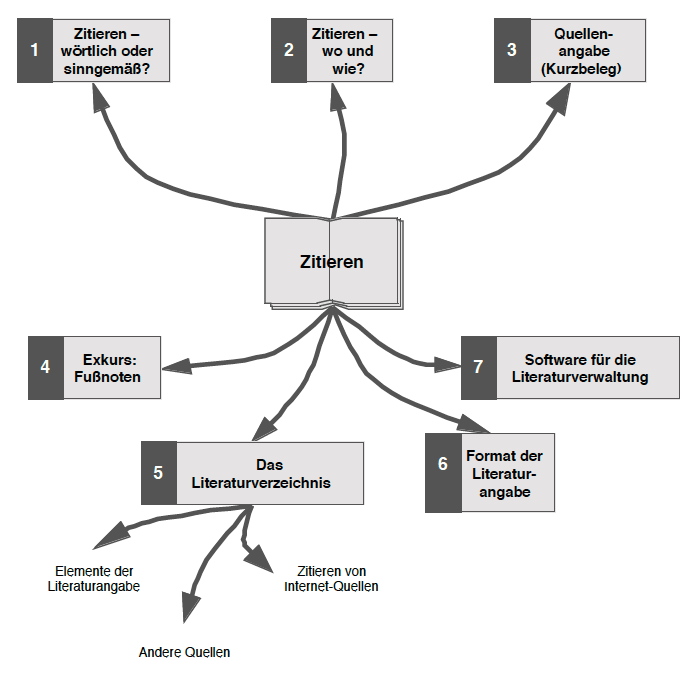
\includegraphics{images/zitieren-min} 

}

\caption{Zitieren (Überblick)}\label{fig:unnamed-chunk-22}
\end{figure}

Mit Ihrer wissenschaftlichen Arbeit liefern Sie einen Beitrag zum
wissenschaftlichen Diskurs. Sie setzen sich beim Lesen und Schreiben mit
den Gedanken und Werken anderer Autoren auseinander und bauen Ihre
Argumentation auf fremden Überlegungen auf. Eigene und fremde Gedanken
sollen sich zu einem neuen Werk verbinden, ohne sich zu vermischen. Beim
Schreiben stellen Sie diese fremden Positionen dar, bewerten und
diskutieren Sie und antworten darauf.

Die Regeln für das richtige Zitieren sollen sicherstellen, dass eigene
und fremde Gedanken sauber voneinander getrennt werden, denn es gibt
beim wissenschaftlichen Arbeiten keine größere „Sünde`` als das Plagiat
(Abschreiben). Darüber hinaus muss Ihre Rezeption fremder Werke
überprüfbar und nachvollziehbar sein, so dass jede Leserin, wenn sie
will, selbst die Quellen konsultieren kann, die Sie benutzt haben. Wenn
man sich den Zweck der Zitierregeln und vor allem die Bedürfnisse der
Leserinnen vor Augen hält, wird man selbst in Zweifelsfällen eine klare
Linie finden: was muss der Leser wissen und wie teile ich es ihm am
besten mit?

In diesem Kapitel geht es um zwei Hauptthemen:

\begin{itemize}
\tightlist
\item
  Wie gibt man Aussagen anderer Autoren wieder?
\item
  Wie belegt man die Herkunft dieser Aussagen?
\end{itemize}

Dabei gehen wir besonders auf folgende häufige Fragen und Probleme ein:

\begin{itemize}
\tightlist
\item
  Warum wird in wissenschaftlichen Arbeiten von Studierenden soviel
  wörtlich zitiert? Was ist das Problem damit und wie lässt es sich
  lösen?
\item
  Wann soll ich wörtlich zitieren, wann ist die Wiedergabe mit eigenen
  Worten besser?
\item
  Welche Methoden gibt es, um wörtlich zu zitieren, und wann verwende
  ich welche? Welche Probleme können dabei auftreten, und wie sind sie
  zu lösen?
\item
  Wie (wie genau, wie oft) muss ich angeben, woher ein Zitat stammt?
  (Quellenangabe)
\item
  Wozu und wann brauche ich Fußnoten?
\item
  Wie gestalte ich das Literaturverzeichnis (Bibliografie), und welche
  Probleme können dabei auftreten?
\item
  Wie kann ich mir diese Arbeit mit dem Computer erleichtern?
\end{itemize}

\section{Zitieren -- wörtlich oder
sinngemäß?}\label{zitieren-wortlich-oder-sinngema}

Viele Seminar- und Diplomarbeiten sehen aus wie Zitatensammlungen: ein
wörtliches Zitat folgt dem anderen, die eigenen Worte des Verfassers
beschränken sich auf ein paar verbindende Sätze, die im Extremfall auch
nur wiederholen, was die zitierten Autoren sagen. Oft finden sich auch
mehrere Zitate mit ein und derselben Kernaussage, nur eben in etwas
anderer Formulierung.

Zwar genügt eine solche Arbeit meist den formalen Spielregeln -- es wird
brav, genau, mit Quellenangaben und Literaturverzeichnis zitiert -- aber
der Sinn und Zweck der Übung, nämlich die Verarbeitung und
Auseinandersetzung mit diesen Autoren und ihren Argumenten, der Diskurs,
ist dabei zu kurz gekommen.

Darüber hinaus ist so eine Arbeit im Extremfall auch kaum lesbar: Der
dauernde Wechsel in Stil und Begrifflichkeit, den das wörtliche Zitieren
mit sich bringt, macht es schwer, eine möglicherweise vom Verfasser
dabei verfolgte Linie zu erkennen, wenn er sich selbst so sehr
zurückhält. Der Verfasser ist weder Teilnehmer an der Diskussion noch
ihr Moderator, sondern agiert eher wie ein unbeteiligter Beobachter, der
alle anderen zu Wort kommen lässt, aber selbst zum Inhalt der Diskussion
nichts beiträgt.

Die Ursachen für diesen Rückzug auf den „Beobachterposten`` im
wissenschaftlichen Diskurs liegen meist schon in der Arbeit, die vor dem
eigentlichen Abfassen des Textes geleistet worden ist. Sie sind daher
beim Schreiben selbst nur mehr zum Teil behebbar.

\begin{longtable}[]{@{}ll@{}}
\caption{\textbf{\label{tab:paraphrasieren} Wörtliche Zitate
reduzieren}}\tabularnewline
\toprule
\begin{minipage}[b]{0.24\columnwidth}\raggedright\strut
Sie zitieren zu oft wörtlich \ldots{}\strut
\end{minipage} & \begin{minipage}[b]{0.70\columnwidth}\raggedright\strut
Sie können das vermeiden, indem Sie \ldots{}\strut
\end{minipage}\tabularnewline
\midrule
\endfirsthead
\toprule
\begin{minipage}[b]{0.24\columnwidth}\raggedright\strut
Sie zitieren zu oft wörtlich \ldots{}\strut
\end{minipage} & \begin{minipage}[b]{0.70\columnwidth}\raggedright\strut
Sie können das vermeiden, indem Sie \ldots{}\strut
\end{minipage}\tabularnewline
\midrule
\endhead
\begin{minipage}[t]{0.24\columnwidth}\raggedright\strut
wenn Sie glauben, nur so zeigen zu können, was und wieviel Sie gelesen
haben.\strut
\end{minipage} & \begin{minipage}[t]{0.70\columnwidth}\raggedright\strut
das Gelesene mit eigenen Worten wiedergeben (= paraphrasieren). Dadurch
zeigen Sie zusätzlich, dass Sie das Gelesene auch verstanden haben.
\vspace{-6mm}\strut
\end{minipage}\tabularnewline
\begin{minipage}[t]{0.24\columnwidth}\raggedright\strut
wenn Sie beim Lesen und Notieren nur kurze, aus dem Kontext gerissene
Passagen abgeschrieben haben, aus denen sich der Argumentationsgang
nicht mehr rekonstruieren lässt.\strut
\end{minipage} & \begin{minipage}[t]{0.70\columnwidth}\raggedright\strut
analytisch lesen (siehe „Analytisches Lesen``, S. †99 XXX) und beim
Lesen und Notieren (Exzerpieren) bereits ans Schreiben und Argumentieren
denken. \vspace{-6mm}\strut
\end{minipage}\tabularnewline
\begin{minipage}[t]{0.24\columnwidth}\raggedright\strut
wenn Sie beim Lesen und Exzerpieren viel Material gesammelt haben und es
nicht über sich bringen, es wegzulassen -- auch wenn es sich inhaltlich
wiederholt.\strut
\end{minipage} & \begin{minipage}[t]{0.70\columnwidth}\raggedright\strut
das treffendste Zitat wörtlich wiedergeben und auf andere Autoren, die
Ähnliches gesagt haben, nur kurz verweisen. \vspace{-6mm}\strut
\end{minipage}\tabularnewline
\begin{minipage}[t]{0.24\columnwidth}\raggedright\strut
wenn Sie nicht sicher sind, ob Sie den Inhalt mit eigenen Worten richtig
und treffend wiedergeben können.\strut
\end{minipage} & \begin{minipage}[t]{0.70\columnwidth}\raggedright\strut
bereits beim Lesen (z. B. durch Rekapitulieren in eigenen Worten)
kontrollieren, ob Sie den Inhalt wirklich verstanden haben. Lexika,
Einführungsbücher etc. helfen dabei, Sicherheit im Umgang mit den
Begriffen und Fachausdrücken zu gewinnen; Paraphrasieren üben.\strut
\end{minipage}\tabularnewline
\bottomrule
\end{longtable}

Wenn Sie aber finden, dass Sie etwas mit eigenen Worten einfach nicht
besser sagen können -- dann ist ein wörtliches Zitat angebracht! Es gibt
auch noch weitere Fälle, in denen ein wörtliches Zitat sinnvoll und
notwendig ist:

\begin{itemize}
\tightlist
\item
  Passagen, wo die exakte Wortwahl und Formulierung des Autors wichtig
  sind, treffende Aussagen, die durch sinngemäße Wiedergabe an Wirkung
  verlieren würden, Schlüsselsätze oder -passagen, die für einen
  Argumentationsgang, ein ganzes Werk oder einen Autor bezeichnend sind.
\item
  Texte, die Gegenstand Ihrer Arbeit sind, und die Sie ausführlich
  analysieren, interpretieren usw. Sind sie länger als eine Seite,
  sollten sie im Anhang der Arbeit beigefügt werden -- trotzdem kann es
  sinnvoll sein, einzelne (Ab)Sätze auch im Text zu zitieren, um dem
  Leser dauerndes Vor- und Zurückblättern zu ersparen.
\item
  Texte, die für den Leser schwer oder gar nicht zugänglich sind. Zwar
  ist es ein Prinzip des wissenschaftlichen Arbeitens, dass es für den
  Leser nachvollziehbar und überprüfbar sein soll. Der Wert mancher
  Arbeiten liegt aber gerade darin, solche Quellen (z. B. längst
  vergriffene oder in Vergessenheit geratene Bücher) zu erschließen.
\item
  Wörtlich zitieren Sie auch mündliche Aussagen, Tonbandaufnahmen von
  einem Vortrag etc. -- solche nicht zugänglichen und nicht
  überprüfbaren Quellen sollten aber nur verwendet werden, wenn es keine
  andere (schriftliche, veröffentlichte) Quelle gibt.
\end{itemize}

\begin{longtable}[]{@{}l@{}}
\caption{\textbf{\label{tab:zitieren} Richtige zitieren}}\tabularnewline
\toprule
\begin{minipage}[t]{0.97\columnwidth}\raggedright\strut
\begin{itemize}
\tightlist
\item
  Ist die Arbeit eine Ansammlung von wörtlichen Zitaten? \vspace{-6mm}
  \textbar{}
  +----------------------------------------------------------------------------------------------------------------------------------+
\item
  Ist das wörtliche Zitieren dort, wo es verwendet wird, für die Leserin
  notwenig und nützlich? \vspace{-6mm}
\end{itemize}\strut
\end{minipage}\tabularnewline
\begin{minipage}[t]{0.97\columnwidth}\raggedright\strut
\begin{itemize}
\tightlist
\item
  Suche ich schon beim Lesen und Notieren nach eigenen Formulierungen?
  \vspace{-6mm}
\end{itemize}\strut
\end{minipage}\tabularnewline
\begin{minipage}[t]{0.97\columnwidth}\raggedright\strut
\begin{itemize}
\tightlist
\item
  Habe ich das Gelesene wirklich verstanden und kann es mit eigenen
  Worten wiedergeben? \vspace{-6mm}
\end{itemize}\strut
\end{minipage}\tabularnewline
\begin{minipage}[t]{0.97\columnwidth}\raggedright\strut
\begin{itemize}
\tightlist
\item
  Sind die wörtlichen Zitate in den Text integriert, d. h. eingeleitet,
  kommentiert und ausgewertet? \vspace{-6mm}
\end{itemize}\strut
\end{minipage}\tabularnewline
\begin{minipage}[t]{0.97\columnwidth}\raggedright\strut
\begin{itemize}
\tightlist
\item
  Ist bei allen Zitaten (nicht nur den wörtlichen) klar ersichtlich,
  dass es Zitate sind und woher sie stammen?
\end{itemize}\strut
\end{minipage}\tabularnewline
\bottomrule
\end{longtable}

\section{Zitieren -- wo und wie?}\label{zitieren-wo-und-wie}

In diesem Abschnitt geht es um den Einbau von wörtlichen Zitaten in den
Text: Wo stehen die Satzzeichen? Wohin gehört die Quellenangabe
(Kurzbeleg)? Das lässt sich am besten darstellen, wenn wir die Zitate
nach ihrer Länge in drei Gruppen einteilen:

\begin{longtable}[]{@{}lll@{}}
\caption{\textbf{\label{tab:zitieren2} Wörtlich zitieren}}\tabularnewline
\toprule
\begin{minipage}[b]{0.13\columnwidth}\raggedright\strut
Sie verwenden \ldots{}\strut
\end{minipage} & \begin{minipage}[b]{0.41\columnwidth}\raggedright\strut
nach dem Muster \ldots{}\strut
\end{minipage} & \begin{minipage}[b]{0.38\columnwidth}\raggedright\strut
Hinweise\strut
\end{minipage}\tabularnewline
\midrule
\endfirsthead
\toprule
\begin{minipage}[b]{0.13\columnwidth}\raggedright\strut
Sie verwenden \ldots{}\strut
\end{minipage} & \begin{minipage}[b]{0.41\columnwidth}\raggedright\strut
nach dem Muster \ldots{}\strut
\end{minipage} & \begin{minipage}[b]{0.38\columnwidth}\raggedright\strut
Hinweise\strut
\end{minipage}\tabularnewline
\midrule
\endhead
\begin{minipage}[t]{0.13\columnwidth}\raggedright\strut
1. \emph{kurze Zitate} (einzelne Begriffe, Wendungen und
Satzteile)\strut
\end{minipage} & \begin{minipage}[t]{0.41\columnwidth}\raggedright\strut
Text „Zitat`` Text. (Quelle) ; Text „Zitat`` (Quelle) Text.; Text
„Zitat``. (Quelle)\strut
\end{minipage} & \begin{minipage}[t]{0.38\columnwidth}\raggedright\strut
wichtig ist der ungebrochene Lesefluss; Grammatik muss zusammenpassen;
Satzzeichen außerhalb der Anführungszeichen \vspace{-6mm}\strut
\end{minipage}\tabularnewline
\begin{minipage}[t]{0.13\columnwidth}\raggedright\strut
2. \emph{mittlere Zitate} (ganze Sätze von maximal 1 -- 2 Zeilen
Länge)\strut
\end{minipage} & \begin{minipage}[t]{0.41\columnwidth}\raggedright\strut
Text. „Zitat.`` (Quelle) Text.; Text: „Zitat.`` (Quelle) ; Einleitung:
„Zitat.`` (Quelle)\strut
\end{minipage} & \begin{minipage}[t]{0.38\columnwidth}\raggedright\strut
Satzzeichen innerhalb der Anführungszeichen! Einleitungen ( wie
„\ldots{} schreibt:`` „\ldots{} sagt:``) vermeiden bzw. variieren
\vspace{-6mm}\strut
\end{minipage}\tabularnewline
\begin{minipage}[t]{0.13\columnwidth}\raggedright\strut
3. lange Zitate (Absätze und lange Sätze)\strut
\end{minipage} & \begin{minipage}[t]{0.41\columnwidth}\raggedright\strut
Text Zitat. (Quelle) Text\strut
\end{minipage} & \begin{minipage}[t]{0.38\columnwidth}\raggedright\strut
Blockzitat; Abstand oben und unten, kleinere Schrift (2 Pkt.), keine
Anführungszeichen, beidseitige Einrückung\strut
\end{minipage}\tabularnewline
\bottomrule
\end{longtable}

Mit der Quellenangabe (Kurzbeleg) beschäftigen wir uns später in diesem
Kapitel, hier wollen wir häufige Zitier-Probleme zusammenfassen.

\begin{longtable}[]{@{}lll@{}}
\caption{\textbf{\label{tab:zitieren3} Sonderfälle des wörtlichen
Zitierens}}\tabularnewline
\toprule
\begin{minipage}[b]{0.13\columnwidth}\raggedright\strut
Wenn \ldots{}\strut
\end{minipage} & \begin{minipage}[b]{0.41\columnwidth}\raggedright\strut
können Sie \ldots{}\strut
\end{minipage} & \begin{minipage}[b]{0.38\columnwidth}\raggedright\strut
wie?\strut
\end{minipage}\tabularnewline
\midrule
\endfirsthead
\toprule
\begin{minipage}[b]{0.13\columnwidth}\raggedright\strut
Wenn \ldots{}\strut
\end{minipage} & \begin{minipage}[b]{0.41\columnwidth}\raggedright\strut
können Sie \ldots{}\strut
\end{minipage} & \begin{minipage}[b]{0.38\columnwidth}\raggedright\strut
wie?\strut
\end{minipage}\tabularnewline
\midrule
\endhead
\begin{minipage}[t]{0.13\columnwidth}\raggedright\strut
das Zitat zu lang und nicht als Ganzes relevant ist\strut
\end{minipage} & \begin{minipage}[t]{0.41\columnwidth}\raggedright\strut
das Zitat kürzen, ohne den Sinn zu entstellen (Ellipse)\strut
\end{minipage} & \begin{minipage}[t]{0.38\columnwidth}\raggedright\strut
Auslassungszeichen: „ \ldots{} '' (Leerzeichen, 3 Punkte, Leerzeichen)
\vspace{-6mm}\strut
\end{minipage}\tabularnewline
\begin{minipage}[t]{0.13\columnwidth}\raggedright\strut
das Zitat einer Erläuterung bedarf (z. B. ein Pronomen enthält)\strut
\end{minipage} & \begin{minipage}[t]{0.41\columnwidth}\raggedright\strut
das Zitat ergänzen, aber nur sinngemäß (Interpolation)\strut
\end{minipage} & \begin{minipage}[t]{0.38\columnwidth}\raggedright\strut
eckige Klammern u. Autoreninitialen: „ Sie {[}die Sophisten, pb{]}
behaupteten \ldots{} '' \vspace{-6mm}\strut
\end{minipage}\tabularnewline
\begin{minipage}[t]{0.13\columnwidth}\raggedright\strut
das Zitat in Englisch ist\strut
\end{minipage} & \begin{minipage}[t]{0.41\columnwidth}\raggedright\strut
das Zitat in Englisch belassen (Englisch kann inzwischen in den meisten
Fächern vorausgesetzt werden)\strut
\end{minipage} & \begin{minipage}[t]{0.38\columnwidth}\raggedright\strut
am besten als ganzer Satz oder Absatz; Einbau in einen deutschen Satz
nur wenn Grammatik nahtlos zusammenpasst (Zahl, Genus, Wortstellung
\ldots{}); nicht mehrmals im Satz zwischen Deutsch und Fremdsprache
wechseln. \vspace{-6mm}\strut
\end{minipage}\tabularnewline
\begin{minipage}[t]{0.13\columnwidth}\raggedright\strut
das Zitat in einer anderen Fremdsprache ist\strut
\end{minipage} & \begin{minipage}[t]{0.41\columnwidth}\raggedright\strut
„facheigene`` Sprachen im Original stehenlassen (zB Französisch in
Romanistik), „fachfremde`` übersetzen.\strut
\end{minipage} & \begin{minipage}[t]{0.38\columnwidth}\raggedright\strut
a) eigene Übersetzung als sinngemäßes Zitat, Original evt. in Fußnote;
b) Zitat im Original, Übersetzung in Fußnote \vspace{-6mm}\strut
\end{minipage}\tabularnewline
\begin{minipage}[t]{0.13\columnwidth}\raggedright\strut
das Zitat aus einem einzelnen Wort besteht, das in der Endung nicht
„passt``\strut
\end{minipage} & \begin{minipage}[t]{0.41\columnwidth}\raggedright\strut
a) die Endung weglassen und nur den Stamm zitieren; b) nötige Endung
hinzufügen\strut
\end{minipage} & \begin{minipage}[t]{0.38\columnwidth}\raggedright\strut
a) keine Auslassungszeichen notwendig; b) Endung interpolieren (in
eckigen Klammern) \vspace{-6mm}\strut
\end{minipage}\tabularnewline
\begin{minipage}[t]{0.13\columnwidth}\raggedright\strut
im Original etwas hervorgehoben ist\strut
\end{minipage} & \begin{minipage}[t]{0.41\columnwidth}\raggedright\strut
Hervorhebung übernehmen, evt. Anmerkung, um klarzumachen, dass es nicht
Ihre Hervorhebung ist\strut
\end{minipage} & \begin{minipage}[t]{0.38\columnwidth}\raggedright\strut
eigene Art der Hervorhebung darf verwendet werden (z. B. kursiv für
fett); Anmerkung {[}Hervorhebung im Original{]}, va. wenn auch eigene
Hervorhebungen vorkommen (s. unten) \vspace{-6mm}\strut
\end{minipage}\tabularnewline
\begin{minipage}[t]{0.13\columnwidth}\raggedright\strut
Sie im Zitat etwas hervorheben wollen\strut
\end{minipage} & \begin{minipage}[t]{0.41\columnwidth}\raggedright\strut
Hervorhebung und Anmerkung mit Autoreninitialen am Ende des Zitats\strut
\end{minipage} & \begin{minipage}[t]{0.38\columnwidth}\raggedright\strut
kursiv; Anmerkung {[}Hervorhebung von mir{]} oder {[}Hervorhebung pb{]}
\vspace{-6mm}\strut
\end{minipage}\tabularnewline
\begin{minipage}[t]{0.13\columnwidth}\raggedright\strut
im Zitat etwas falsch, veraltet oder unüblich geschrieben ist\strut
\end{minipage} & \begin{minipage}[t]{0.41\columnwidth}\raggedright\strut
die Schreibweise übernehmen, Hinweis unmittelbar anfügen\strut
\end{minipage} & \begin{minipage}[t]{0.38\columnwidth}\raggedright\strut
Hinweis {[}sic{]} oder {[}!{]} anfügen; „sic`` ist keine Abkürzung und
bedeutet „so steht es im Original``\strut
\end{minipage}\tabularnewline
\bottomrule
\end{longtable}

Die sinngemäße Wiedergabe (Paraphrase) einer Passage aus einem fremden
Werk ist in jedem dieser Fälle ebenfalls eine Möglichkeit,
Schwierigkeiten zu umgehen. Paraphrasen fügen sich, da Sie sie selbst
formulieren, besser in Ihren eigenen Text ein und helfen das Problem der
„Zitatensammlung`` vermeiden. Es darf dabei aber keinesfalls vergessen
werden, dass auch Paraphrasen Zitate sind und belegt werden müssen.

\section{Quellenangabe (Kurzbeleg)}\label{quellenangabe-kurzbeleg}

Bei jedem Zitat -- gleich ob wörtlich oder sinngemäß -- muss angegeben
werden, woher es stammt. Dazu gibt es verschiedene Methoden, wie etwa
Fußnoten, Endnoten oder Kurzbelege im Text. Wir beschreiben hier die
inzwischen fast allgemein übliche Harvard-Notation`` mit Kurzbelegen,
die wir empfehlen, wenn man sich die Methode der Quellenangabe frei
aussuchen kann. Wenn aber z. B. der Fachbereich oder der Verlag ein
anderes System vorschreiben, muss man sich natürlich daran halten. Als
Grundform der Harvard-Notation kann gewählt werden:

A\texttt{\{r\ fig.align=\textquotesingle{}center\textquotesingle{},\ echo=FALSE,\ fig.cap=\textquotesingle{}Grundmuster\ des\ Kurzbelegs\textquotesingle{}\}\ knitr::include\_graphics(\textquotesingle{}images/zitieren-grundform-min.png\textquotesingle{},\ dpi\ =\ NA)}

Grundsätze bei der Verwendung von Kurzbelegen sind:

\begin{itemize}
\tightlist
\item
  Konsistenz: Gleich, welche dieser Formen Sie wählen (wobei sich der
  Doppelpunkt durchzusetzen scheint), Sie müssen sie in der gesamten
  Arbeit beibehalten.
\item
  Eindeutigkeit: Der Kurzbeleg muss so abgefasst sein, dass das zitierte
  Werk in der Literaturliste eindeutig identifiziert werden kann.
\item
  Literaturverzeichnis: Zu diesen Kurzbelegen gehört notwendig ein
  Literaturverzeichnis, in dem die volle Quellenangabe anhand des
  Kurzbelegs zweifelsfrei und mühelos gefunden werden kann.
\item
  Kürze: Der Kurzbeleg soll tatsächlich so kurz wie möglich sein, alle
  unnötigen Wiederholungen sind zu vermeiden. Daher gibt es zur
  Grundform noch weiter abgekürzte Varianten.
\end{itemize}

Die wichtigsten Fragen und Zweifelsfälle dazu sind in der folgenden
Tabelle zusammengefasst:

\begin{longtable}[]{@{}lll@{}}
\caption{\textbf{\label{tab:zitieren3} Kurzbelege verwenden}}\tabularnewline
\toprule
\begin{minipage}[b]{0.18\columnwidth}\raggedright\strut
Frage \ldots{}\strut
\end{minipage} & \begin{minipage}[b]{0.37\columnwidth}\raggedright\strut
Antwort\strut
\end{minipage} & \begin{minipage}[b]{0.36\columnwidth}\raggedright\strut
Beispie(e)\strut
\end{minipage}\tabularnewline
\midrule
\endfirsthead
\toprule
\begin{minipage}[b]{0.18\columnwidth}\raggedright\strut
Frage \ldots{}\strut
\end{minipage} & \begin{minipage}[b]{0.37\columnwidth}\raggedright\strut
Antwort\strut
\end{minipage} & \begin{minipage}[b]{0.36\columnwidth}\raggedright\strut
Beispie(e)\strut
\end{minipage}\tabularnewline
\midrule
\endhead
\begin{minipage}[t]{0.18\columnwidth}\raggedright\strut
Wo steht der Kurzbeleg?\strut
\end{minipage} & \begin{minipage}[t]{0.37\columnwidth}\raggedright\strut
so nah am Zitat wie möglich, ohne den Lesefluss zu stören, und so nah
wie nötig, um eindeutig zuordenbar zu sein.\strut
\end{minipage} & \begin{minipage}[t]{0.36\columnwidth}\raggedright\strut
Es werden dafür auch die Begriffe „ABC`` (Müller 1998) und „XYZ`` (Meier
1999) verwendet. ; Es wird dafür auch der Begriff „ABC`` verwendet.
(Schmidt 1997) \vspace{-6mm}\strut
\end{minipage}\tabularnewline
\begin{minipage}[t]{0.18\columnwidth}\raggedright\strut
Was tun, wenn zwei gleichnamige Autoren vorkommen?\strut
\end{minipage} & \begin{minipage}[t]{0.37\columnwidth}\raggedright\strut
Initialen anfügen, selbst wenn die Werke durch die Jahreszahl
unterscheidbar wären\strut
\end{minipage} & \begin{minipage}[t]{0.36\columnwidth}\raggedright\strut
(Müller J. 1991:127) und (Müller H. 1987:36) \vspace{-6mm}\strut
\end{minipage}\tabularnewline
\begin{minipage}[t]{0.18\columnwidth}\raggedright\strut
Wie sieht der Kurzbeleg für ein Werk mehrerer Autoren aus?\strut
\end{minipage} & \begin{minipage}[t]{0.37\columnwidth}\raggedright\strut
Zwei Namen müssen, drei Namen können angeführt werden; ab 3 Namen: 1.
Name (wenn eindeutig) und „et al.`` anfügen\strut
\end{minipage} & \begin{minipage}[t]{0.36\columnwidth}\raggedright\strut
(Müüler und Mayer 2003)\strut
\end{minipage}\tabularnewline
\begin{minipage}[t]{0.18\columnwidth}\raggedright\strut
(Müller, Mayr \& Schmidt 1993:124) bzw. (Müller et al. 1993:124)
\vspace{-6mm}\strut
\end{minipage} & \begin{minipage}[t]{0.37\columnwidth}\raggedright\strut
\strut
\end{minipage}\tabularnewline
\begin{minipage}[t]{0.18\columnwidth}\raggedright\strut
Wie unterscheidet man Werke eines Autors mit demselben
Erscheinungsjahr?\strut
\end{minipage} & \begin{minipage}[t]{0.37\columnwidth}\raggedright\strut
Buchstaben a, b, c an das Jahr anhängen, u. zw. in der Reihenfolge der
Erwähnung im Text\strut
\end{minipage} & \begin{minipage}[t]{0.36\columnwidth}\raggedright\strut
(Maier 1992a:231-4) \ldots{} einige Seiten später \ldots{} (Maier
1992b:27) \vspace{-6mm}\strut
\end{minipage}\tabularnewline
\begin{minipage}[t]{0.18\columnwidth}\raggedright\strut
Kann man auch auf ein Werk insgesamt, ohne Seitenangaben
verweisen?\strut
\end{minipage} & \begin{minipage}[t]{0.37\columnwidth}\raggedright\strut
Ja, wenn man sich auf ein gesamtes Werk bezieht. Der Kurzbeleg bleibt
dann ohne Seitenzahl, evt. „Vgl.``, „cf.`` oder kurze Anmerkung
voranstellen. Elektronische Quellen haben oft keine Seitenzahlen.\strut
\end{minipage} & \begin{minipage}[t]{0.36\columnwidth}\raggedright\strut
(cf.~Müller 1991) \ldots{} (Vgl. dazu auch Maier 1994) \ldots{}
(ausführlicher dazu Schmidt 1990) \vspace{-6mm}\strut
\end{minipage}\tabularnewline
\begin{minipage}[t]{0.18\columnwidth}\raggedright\strut
Wie hängt man mehrere Kurzbelege aneinander?\strut
\end{minipage} & \begin{minipage}[t]{0.37\columnwidth}\raggedright\strut
in einer gemeinsamen Klammer\strut
\end{minipage} & \begin{minipage}[t]{0.36\columnwidth}\raggedright\strut
(Vgl. Müller 1991, Mayr 1993 und Schmidt 1995) \vspace{-6mm}\strut
\end{minipage}\tabularnewline
\begin{minipage}[t]{0.18\columnwidth}\raggedright\strut
Wie erwähnt man mehrere Werke eines Autors in einem Kurzbeleg?\strut
\end{minipage} & \begin{minipage}[t]{0.37\columnwidth}\raggedright\strut
Nach dem Prinzip „Keine Verdopplungen`` -- nur Jahreszahlen\strut
\end{minipage} & \begin{minipage}[t]{0.36\columnwidth}\raggedright\strut
(Vgl. Schmidt 1991a und b, sowie 1993) \vspace{-6mm}\strut
\end{minipage}\tabularnewline
\begin{minipage}[t]{0.18\columnwidth}\raggedright\strut
Wie gibt man einen Seitenbereich statt einer einzigen Seitenzahl
an?\strut
\end{minipage} & \begin{minipage}[t]{0.37\columnwidth}\raggedright\strut
mit Binde-Strich und auf das Notwendigste gekürzt; auch „f.`` (folgende
Seite) und „ff.`` (ferner folgende Seiten) sind erlaubt, aber
ungenauer\strut
\end{minipage} & \begin{minipage}[t]{0.36\columnwidth}\raggedright\strut
(Müller 1992:351--3); (Mayr 1994:359--61); (Schmidt 1987:124f.)
\vspace{-6mm}\strut
\end{minipage}\tabularnewline
\begin{minipage}[t]{0.18\columnwidth}\raggedright\strut
Was tun, wenn der Kurzbeleg unsinnig wirkt, wie z. B. bei bekannten
alten, aber neu aufgelegten Werken wie (Grimmelshausen 1993) oder
(Rousseau 1965)?\strut
\end{minipage} & \begin{minipage}[t]{0.37\columnwidth}\raggedright\strut
Im Kurzbeleg kann das tatsächliche Erscheinungsjahr stehen, das
Literaturverzeichnis muss allerdings auch genau die verwendete Ausgabe
enthalten\strut
\end{minipage} & \begin{minipage}[t]{0.36\columnwidth}\raggedright\strut
(Grimmelshausen 1668) ; (Rousseau 1753) ; (zu den Angaben im
Literaturverzeichnis siehe unten) \vspace{-6mm}\strut
\end{minipage}\tabularnewline
\begin{minipage}[t]{0.18\columnwidth}\raggedright\strut
Muss der Kurzbeleg jedes mal so gemacht werden, auch wenn immer wieder
aus demselben Werk zitiert wird?\strut
\end{minipage} & \begin{minipage}[t]{0.37\columnwidth}\raggedright\strut
Alles, was sich wiederholen würde, kann wegbleiben, solange für den
Leser die Quelle klar ist. Es genügt die Seitenangabe, oder sogar ein
„ebd.``, wenn auch die Seite unverändert bleibt.\strut
\end{minipage} & \begin{minipage}[t]{0.36\columnwidth}\raggedright\strut
1. Zitat (Müller 1991:351) \ldots{} 2. Zitat (S. 353) \ldots{} 3. Zitat
(ebd.). \emph{aber} ein paar Seiten später: 4. Zitat (Müller 1991:123)
\vspace{-6mm}\strut
\end{minipage}\tabularnewline
\begin{minipage}[t]{0.18\columnwidth}\raggedright\strut
Muss der Kurzbeleg komplett angegeben werden, wenn Teile davon schon im
Text erwähnt sind?\strut
\end{minipage} & \begin{minipage}[t]{0.37\columnwidth}\raggedright\strut
Es genügen immer jene Angaben, die zur vollständigen Identifizierung
noch fehlen.\strut
\end{minipage} & \begin{minipage}[t]{0.36\columnwidth}\raggedright\strut
Müller betont, dass „Zitat`` (1991:351). ; Mayr vertrat schon 1956 die
Auffassung, dass „Zitat`` (S. 124). \vspace{-6mm}\strut
\end{minipage}\tabularnewline
\begin{minipage}[t]{0.18\columnwidth}\raggedright\strut
Wie werden Werke zitiert, die nur unter ihrem Titel bekannt sind?\strut
\end{minipage} & \begin{minipage}[t]{0.37\columnwidth}\raggedright\strut
nach dem Ordnungswort, unter dem sie auch im Literaturverzeichnis
erscheinen. Konversationslexika u. dgl. brauchen nicht zitiert zu
werden!\strut
\end{minipage} & \begin{minipage}[t]{0.36\columnwidth}\raggedright\strut
(Fischer Weltalmanach 1988:117) \vspace{-6mm}\strut
\end{minipage}\tabularnewline
\begin{minipage}[t]{0.18\columnwidth}\raggedright\strut
Ist es möglich, eine Abkürzung des Titels statt des Kurzbelegs zu
verwenden, wenn ein Werk oft zitiert wird?\strut
\end{minipage} & \begin{minipage}[t]{0.37\columnwidth}\raggedright\strut
Wenn Werke eingehend analysiert werden (= Gegenstand der Arbeit sind),
kann ein Stichwort oder eine standardisierte Abkürzung verwendet werden;
die Jahreszahl bleibt weg.\strut
\end{minipage} & \begin{minipage}[t]{0.36\columnwidth}\raggedright\strut
(TKH:214--18) statt (Habermas 1981:214--18); (cf.~GB) statt (cf.~Chomsky
1981) \vspace{-6mm}\strut
\end{minipage}\tabularnewline
\begin{minipage}[t]{0.18\columnwidth}\raggedright\strut
Darf man solche Abkürzungen selbst erfinden, und wie führt man sie
ein?\strut
\end{minipage} & \begin{minipage}[t]{0.37\columnwidth}\raggedright\strut
Nur wenn es nicht bereits eine fachintern übliche gibt, und nur für
Werke, die in der Arbeit eine zentrale Rolle spielen. Beim ersten Zitat
normaler Kurzbeleg u. Hinweis auf Abkürzung; evt.
Abkürzungsverzeichnis\strut
\end{minipage} & \begin{minipage}[t]{0.36\columnwidth}\raggedright\strut
1. Zitat (Habermas 1981:103, im folgenden TKH) \ldots{} 2. Zitat
(TKH:105). (TKH = Theorie des kommunikativen Handelns) ; In den
„Lectures on Government and Binding`` (Chomsky 1981, im folgenden mit GB
abgekürzt) \ldots{}\strut
\end{minipage}\tabularnewline
\bottomrule
\end{longtable}

\section{Exkurs: Fußnoten}\label{exkurs-funoten}

Mit der hier beschriebenen Methode des Kurzbelegs fallen alle Fußnoten
mit Literaturhinweisen weg. Der Leser muss nicht zwischen Text und dem
Fuß der Seite (oder gar -- bei Endnoten -- dem Ende des Buchs) hin- und
herspringen, nur um dort ein kryptisches „ebd.`` oder „a.a.O.`` zu
finden, das ihn zwingt, die erste auf dieses Werk bezogene Fußnote durch
Herumblättern zu suchen.

Sind Fußnoten damit völlig überflüssig geworden? Durchaus nicht. Im
Gegenteil -- die Fußnote kann ihren eigentlichen Zweck nun besser
erfüllen. Der besteht darin, Anmerkungen, Zusätze, kleine Exkurse und
Erläuterungen aufzunehmen, die im (Haupt-)Argumentationsgang nichts
verloren haben oder ihn unnötig aufblähen würden. Da die Quellenangaben
sämtlich im Text untergebracht sind, kann sich der Leser jetzt, wenn er
auf ein Fußnotenzeichen trifft, auf jeden Fall eine inhaltliche
Bemerkung erwarten.

\begin{figure}

{\centering 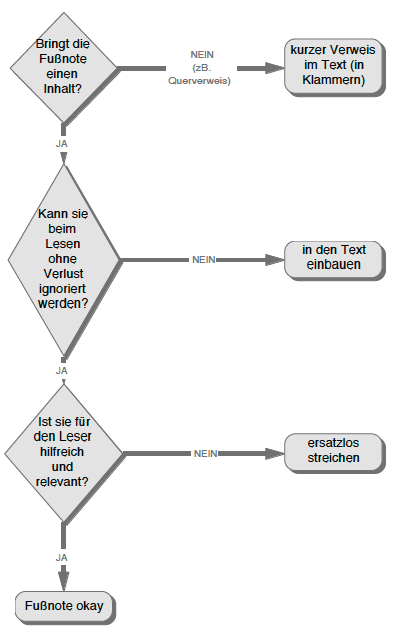
\includegraphics{images/zitieren-fussnote-min} 

}

\caption{Entscheidungsbaum: Fußnoten}\label{fig:unnamed-chunk-23}
\end{figure}

Einen Anwendungsfall für Fußnoten haben wir bereits erwähnt: die
Übersetzung eines fremdsprachigen Zitats (bzw. das fremdsprachige
Original). Ebenso gehören „Überlegungen am Rande`` in Fußnoten. Manche
Wissenschafter haben die Erfahrung gemacht, dass gerade solche Fußnoten,
in denen sie Gedanken oder Fragen formulieren, die noch nicht
abgeschlossen und noch nicht „reif`` für eine ausgearbeitete
Argumentation sind, den Kern ihres nächsten Buches darstellen, weil
ihnen dieser gedankliche „Ausreißer`` keine Ruhe lässt.

Fußnoten sind also nicht überflüssig geworden, aber man sollte trotzdem
so sparsam wie möglich damit umgehen. Wenn Sie beim Schreiben andauernd
den Drang haben, eine Fußnote einzufügen oder etwas aus dem Haupttext in
eine Fußnote zu verbannen, dann kann das ein Hinweis darauf sein, dass
die Argumentation noch nicht „steht``, dass die klare Linie fehlt, oder
dass Sie vielleicht eine ganz andere Arbeit schreiben möchten als die,
an der Sie gerade sitzen (müssen).

\section{Das Literaturverzeichnis}\label{das-literaturverzeichnis}

Das Literaturverzeichnis enthält alle Quellen, die in der Arbeit
verwendet wurden, mit allen Angaben, die notwendig sind, um sie zu
identifizieren und aufzufinden. Zu jedem Kurzbeleg muss es daher einen
Eintrag im Literaturverzeichnis geben. Dieser Eintrag muss dem Kurzbeleg
eindeutig zugeordnet und außerdem schnell und mühelos gefunden werden
können (durch alphabetische Sortierung des Literaturverzeichnisses). Es
genügt daher nicht, bei der Endkorrektur nur stichprobenartig zu prüfen,
ob sich eine Quellenangabe auch im Literaturverzeichnis wiederfindet.
Gerade bei längeren Arbeiten, von denen Teile vielleicht schon früher
verfasst worden sind und nun integriert wurden, stößt man immer wieder
auf Quellen, von denen man schon wieder vergessen hat, dass sie
verwendet wurden. Bewährt hat es sich z. B., in einem Korrekturausdruck
der Arbeit alle Kurzbelege mit Markierstift anzustreichen. Dann kann man
sie beim Durchblättern der Arbeit mit dem Literaturverzeichnis
vergleichen und so Stück für Stück kontrollieren bzw. nötigenfalls
nachtragen.

Andererseits darf das Literaturverzeichnis nur genau jene Quellen
enthalten, die verwendet wurden, und nicht mehr! Studierende glauben
manchmal, dass die Bibliografie eine bestimmte Länge haben muss, damit
die Arbeit positiv bewertet wird, und erliegen der Versuchung, das
Literaturverzeichnis ein wenig zu „strecken``. Dann erscheinen z. B.
Werke im Literaturverzeichnis, die eigentlich nur aus der
Sekundärliteratur zitiert wurden. Ein Zitat aus zweiter Hand ist an und
für sich zulässig, vor allem wenn das Primärwerk nicht verfügbar ist.
Eine Autorin, die eine wichtige Rolle in der Argumentation spielt,
sollten Sie allerdings schon im Original lesen. Schon beim Kurzbeleg
eines solchen Zitats muss die eigentlich verwendete Quelle mit „zitiert
nach \ldots{}`` angegeben werden. Im Literaturverzeichnis darf nur das
tatsächlich verwendete Werk erscheinen.

Es können nur dann alle notwendigen Angaben gemacht werden, wenn diese
auch verfügbar sind. Das bedeutet, dass entliehene Werke sofort mit
allen bibliografischen Daten erfasst werden müssen. Fehlen Angaben, so
muss man entweder das Buch nochmals ausleihen, oder man muss jeden
Verweis auf diese Quelle streichen!

Es gibt zahlreiche verschiedene Formen, wie eine Literaturangabe
geschrieben werden kann. Sie variieren noch dazu je nach der Art der
Quelle, die zitiert wird. Diese Vielfalt von Regeln werden besser
überschaubar, wenn man sich die Literaturangabe wie einen Baukasten
vorstellt, aus dem je nach Bedarf Blöcke zusammengesetzt werden. Die
Grafik zeigt die häufigsten Quellen und ihre Elemente. Zusätze (wie
„In:`` oder „Hg.``) und Stil (wie Unterstreichung oder Kursivschrift)
hängen dann vom jeweiligen (fachüblichen oder vom Verlag geforderten)
Zitierstil ab und werden hier nicht berücksichtigt.

\subsection{Elemente der
Literaturangabe}\label{elemente-der-literaturangabe}

Wir werden zunächst die einzelnen „Bausteine`` der Literaturangabe
erläutern. Autor * Nachname und Vorname (oder Initialen); wenn möglich
und im Format erforderlich, Initialen zu ganzem Vornamen ergänzen (in
eckigen Klammern, z. B. Müller, H{[}einrich{]}. * Mehrere Autoren: Wenn
nur drei angeführt werden dürfen, mit „et al.`` auf weitere Autoren
hinweisen. * Autor völlig unbekannt: {[}anon.{]} als Autor angeben *
Autor nicht namentlich bekannt: durch die herausgebende Institution
ersetzen, z. B. Statistisches Bundesamt (1989): Statistisches Jahrbuch
\ldots{}. , oder Ordnungswort für allgemein bekannte Werke verwenden, z.
B. Fischer Weltalmanach \ldots{} * nur den Namen, keine Titel und
akademischen Grade angeben. Ein „o.Univ.Prof.~Mag.rer.soc.oec. Dr.~phil.
Fritz Müller`` wird als Autor schlicht zu „Müller, Fritz``. * Pseudonyme
werden beibehalten, wenn sie bekannter sind als die „bürgerlichen``
Namen. Diese können in eckigen Klammern angefügt werden, z. B. Novalis
{[}Hardenberg, Friederich Leopold Freiherr von{]}.

\begin{figure}

{\centering 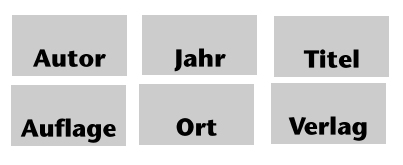
\includegraphics{images/zitieren-buch-min} 

}

\caption{Grundmuster der Literaturangabe}\label{fig:unnamed-chunk-24}
\end{figure}

\begin{itemize}
\tightlist
\item
  Adelsprädikate, mehrteilige Namen: Was fester Bestandteil des Namens
  ist, wird dem Nachnamen vorangestellt, das andere kann dem Vornamen
  folgen, z. B. „Van Dijk, Teun`` aber „Grimmelshausen, Hans Jakob
  Christoph von``. Jahr
\item
  unbekannt: durch „o.J.`` ersetzen
\item
  ungewiss: in eckigen Klammern, mit Fragezeichen: {[}1768?{]}
\item
  aus Sekundärliteratur erschlossen: in eckigen Klammern: {[}1834{]}.
\item
  Tatsächliches Erscheinungsjahr des verwendeten Werks verwenden (im
  Gegensatz zum Kurzbeleg), also: Nietzsche, Friedrich. 1982. Das
  ursprüngliche Erscheinungsjahr kann angefügt werden, z. B. wenn das
  Werk mit dieser Jahresangabe allgemein bekannt ist, also:
  Grimmelshausen, Hans Jakob Christoph von. 1993 (1668). Titel, Auflage
\item
  Ungewöhnlich lange Titel dürfen gekürzt werden; Kürzung durch 3 Punkte
  anzeigen
\item
  Titel und Untertitel dem Titelblatt (im Buch) entnehmen --
  Schmutztitel (dem Titelblatt vorangestellte Seite im Buch) und
  Buchdeckel können unvollständig sein.
\item
  mit dem Titel eines Sammelbandes wird ebenso verfahren.
\item
  abkürzen mit „Aufl.`` (englisch „ed.``)
\item
  besondere Zusätze (dem Titelblatt entnommen) ebenfalls abgekürzt
  davorsetzen, z. B. „3. erw. u. durchges. Aufl.`` Verlag, Ort
\item
  wenn Ortsangabe fehlt: „o. O.``, besser: recherchieren und ergänzen
\item
  bei unterschiedlichen Orten (z. B. der Druckerei): Ort des Verlags
  angeben
\item
  mehrere Ortsangaben (z. B. internationaler Verlag) anführen (meist mit
  Beistrichen getrennt), aber nicht mehr als drei. Herausgeber,
  Übersetzer u. a.
\item
  für Herausgeber gelten im Prinzip die gleichen Regeln wie für Autoren,
  in manchen Formaten werden sie aber (stärker) gekürzt.
\item
  „Hg.`` hinzufügen (englisch Einzahl „ed.`` oder Mehrzahl „eds.``) --
  je nach Format vor dem Namen oder nachher in Klammern
\item
  Spezielle Zusätze wie „Hg. und überarb. von`` möglichst vom Titelblatt
  übernehmen.
\item
  Übersetzer mit „Übs.`` nach dem Titel bzw. nach dem Herausgeber
  anführen Seiten
\item
  meistens ohne vorangestelltes „S.`` (engl. „p.`` bzw. „pp.``)
\item
  genauen Seitenumfang (von -- bis) angeben: 212-217 (oder 212-7)
\item
  Seitenangaben werden nur für unselbständige Werke (Artikel in
  Zeitschriften oder Sammelbänden) gemacht.
\item
  Veröffentlichte Dissertationen und Habilitationsschriften werden wie
  Bücher behandelt. Unveröffentlichte Arbeiten
\item
  Bei unveröffentlichten Arbeiten wird die Institution (Universität und
  Fakultät) angegeben.
\item
  Der Ort geht entweder aus dem Namen der Institution hervor (z. B.
  Universität Wien) oder wird vorangestellt (Wien: Universität für
  Bodenkultur).
\item
  Bei unveröffentlichten Arbeiten wird angegeben, um was für eine Art
  von Arbeit es sich handelt, z. B. „Diss.``, „Habil. Schrift`` oder
  „Diplomarbeit``
\item
  Auch bei internen Reihen (grauen Papieren, Berichten) wird so
  verfahren; Bezeichnung oder Namen der Reihe und evt. Nummer sind am
  Titelblatt zu finden, z. B. „Technical Report 29``; „Zwischenbericht``
  u.dgl. Jahrgang, Heft
\item
  Jahrgänge einer Zeitschrift (volumes) werden entweder durchnummeriert,
  z. B. „34. Jg.`` (engl. „vol.~34``) oder durch die Jahreszahl
  bezeichnet, manchmal auch durch beides.
\item
  Man übernimmt die Jahrgangsbezeichnung, wie sie auf der Zeitschrift
  angegeben ist.
\item
  Die Ausgaben einer Zeitschrift werden entweder für jeden Jahrgang neu
  nummeriert, also z. B. Nr. 3 (1996) = drittes Heft im Jahr 1996 oder
\item
  durchnummeriert, besonders bei Fachzeitschriften.
\item
  Man übernimmt wieder die Angaben so, wie sie auf der Zeitschrift
  angegeben sind.
\end{itemize}

Die folgenden Beispiele sind den Bibliografien wissenschaftlicher Bücher
entnommen und zeigen einige der erläuterten Fälle in der praktischen
Anwendung:

\begin{quote}
Saussure, Ferdinand de. 1967 (1916). Grundfragen der allgemeinen
Sprachwissenschaft. Berlin: Walter de Gruyter \& Co.
\end{quote}

\begin{quote}
Fuchs, Werner/Klima, Rolf/Lautmann, Rüdiger/Rammstedt, Otthein/Wienold,
Hans (Hg.). 1978. Lexikon zur Soziologie. 2., verbesserte und erweiterte
Auflage. Opladen: Westdeutscher Verlag.
\end{quote}

\begin{quote}
Hentke, Reinhard (1987): Handlungsorientierung oder kritische Bildung?
-- Kritik des „handlungs- und situationsorientierten`` Ansatzes der
Wirtschaftsdidaktik. Wirtschaft und Erziehung 39, Nr. 11, S. 354--362.
(Wiederabdruck u. zit. n. Bundesverband der Lehrer an Wirtschaftsschulen
1991, S. 7--21).
\end{quote}

\begin{quote}
Lammer, Christina. 1992. Die Demaskierung des freien Körpers.
Diplomarbeit zur Erlangung des Magistragrades an der grund- und
integrativwissenschaftlichen Fakultät der Universität Wien.
\end{quote}

\subsection{Andere Quellen}\label{andere-quellen}

Bis hier haben wir uns mit den üblichen und am häufigsten verwendeten
gedruckten Quellen beschäftigt. Es kann in einer Arbeit aber notwendig
werden, andere Medien, wie Software, Filme, Websites, persönliche
Mitteilungen oder Rundfunksendungen zu zitieren. Hier sind Hinweise zum
Zitieren solcher Quellen:

Filme werden wie Bücher zitiert, mit dem Regisseur als Autor. Nach dem
Titel wird die Art des Werks angegeben, z. B. „Spielfilm``. Statt dem
Verlag wird der Verleih bzw. Produzent genannt, z. B. „Paramount``. Das
Produktionsjahr wird ebenfalls angeführt, aber statt eines Ortes nur das
Land, in dem der Film produziert wurde. Es ist unerheblich, ob Sie den
Film im Kino, Fernsehen oder von der Videokassette gesehen haben --
diese Angabe ist nicht notwendig. Es kann aber ein hilfreicher Hinweis
für einen Leser sein, der dieses Werk finden will, und Sie können es ihm
zuliebe ohne weiteres angeben.

\begin{quote}
Wenders, Wim. Buena Vista Social Club. Musikfilm. BRD, 1999.
\end{quote}

Fernseh- od. Rundfunksendungen werden mit Regisseur und Titel sowie der
Art, z. B. „Dokumentation``, zitiert. Angabe des Senders und von Datum
und Zeit der Ausstrahlung vervollständigen den Beleg:

\begin{quote}
Wagner, Martin. 1997. Chirurgen am Computer. Neue Wege der Telemedizin.
Dokumentation. ORF 2: 29. 8. 97, 20.15 -- 21.45``.
\end{quote}

Einzelne Teile von Sendungen, z. B. ein Beitrag in einer
Dokumentationsserie, werden wie unselbständige Werke (Artikel)
behandelt: Regisseur, Titel des Beitrags, Serientitel, Sender und
Zeitpunkt.

Nicht bei jeder Software sind die Autoren bekannt. In diesem Fall wird
der Name des Programms als Ordnungswort gewählt (entsprechend dem
Sachtitel von Büchern). Nach Duden würde man einfach die Erläuterung
„Computer-Software`` an den Titel anhängen, wir halten das aber für zu
ungenau -- der Typ der Software, wie „Computerspiel`` oder
„Autorensystem``, ist aufschlussreicher. Die Quellenangabe soll außerdem
enthalten: * \emph{Version}: Die Angabe der Version (und der Sprache)
ist bei Software wichtig. Sie wird so angeführt wie sie bei der Software
verwendet wird, also z. B. „Vers. 5.1D``. * \emph{Hersteller bzw.
Verlag} (im Zweifelsfall: der Inhaber des Copyrights) werden, wenn
möglich mit Ort, wie der Verlag beim Buch angegeben. * Das \emph{Jahr}
ist jenes des Copyrights:

\begin{quote}
Microsoft Word. Vers. 5.1D. Redmond (WA): Microsoft Corparation, 1993.
\end{quote}

\begin{itemize}
\tightlist
\item
  \emph{Speichermedium}: Die Angabe des Speichermediums, z. B. „CD-ROM``
  ist nicht mit dem Softwaretyp zu verwechseln und ersetzt ihn nicht.
  Diese Angabe ist nicht unbedingt notwendig, da die Software dieselbe
  bleibt, gleich auf welchem Medium sie gespeichert wurde. Sie können
  diese Angabe aber -- wie bei der Videokassette -- den Lesern als
  Hilfestellung hinzufügen. Wenn Sie Software zitieren, die Sie aus dem
  Internet heruntergeladen haben, gilt Ähnliches: ist es eine auch
  anders, z. B. über den Handel, erhältliche Software, so muss der
  ftp-Server nicht angegeben werden -- aber er kann (als
  Speichermedium). Gibt es diese Software aber (Ihres Wissens) sonst
  nirgends außer im Internet, dann geben Sie statt Ort und/oder
  Produzent die Server-Adresse und den Pfad in der üblichen URL-Notation
  an, z. B.
\end{itemize}

\begin{quote}
BigPicture 4.2. Shareware. \url{ftp://tuwien.ac.at/tucows/util/mac/}
\end{quote}

\subsection{Zitieren von
Internet-Quellen}\label{zitieren-von-internet-quellen}

Ebenso werden Websites durch ihre URL zitiert. Die Besonderheit daran
ist, dass durch die URL jede einzelne Seite für sich, wie ein
selbständiges Werk, zitiert werden kann. Trotzdem will der Leser
vielleicht gern wissen, in welchem Kontext bzw. zu welchem Server die
zitierte Seite gehört: dann gehen Sie wie beim Zitieren von
unselbständigen Werken vor, aber es genügt als „Bezugsquelle`` die URL
der Seite, da sie die übergeordneten Quellen ja enthält.

Nach dem Style Guide der APA (American Psychological Association, ein in
verschiedenen Wissenschaften weit verbreiteter Standard für die
Erstellung wissenschaftlicher Publikationen) wird der
Literaturverzeichniseintrag einer Webseite in der Grundform dargestellt
als:

\begin{quote}
Autor bzw. Herausgeber. (Datum der letzten Änderung oder des Copyright).
Titel der Seite. Herausgebende Institution. Gsefunden am {[}Datum des
letzten Zugriffs{]} im World Wide Web: URL
\end{quote}

\begin{quote}
Barribeau, S. (29.01.2000). Internet Citation Guides: Citing Electronic
Sources in Research Papers and Bibliographies. University of
Wisconsin-Madison, Memorial Library. Gefunden am 20. April 2000 im World
Wide Web: \url{http://www.library.wisc.edu} /libraries/Memorial/
citing.htm
\end{quote}

Dazu noch einige Erläuterungen zu einzelnen Elementen:

\begin{itemize}
\tightlist
\item
  \emph{Titel}: Der Titel wird so angegeben, wie er im Browser-Fenster
  erscheint (und nicht etwa die HTML-Kurzbezeichnung, wie man sie in den
  Bookmarks wiederfindet). Da untergeordnete Seiten nicht immer einen
  Titel haben, sollte man zum Zitieren in der Hierarchie bis zum Titel
  (bzw. zur Homepage) hinaufgehen.
\item
  \emph{Autor}: Namentliche Verfasser von Web-Seiten sind oft nicht
  leicht zu finden. Meistens sind es Institutionen, die dafür
  verantwortlich zeichnen. Der „Webmaster``, der als Kontaktperson bei
  den meisten Servern angegeben ist, darf nicht automatisch als
  Verfasser angenommen werden. So würde man z. B. angeben:
  \textgreater{} National Science Foundation: Annual Report 1995.
  \url{http://www.nsf.gov/rep95/index.html}.
\item
  \emph{Aktualisierungsdatum}: Ein Problem mit Zitaten aus dem WWW ist,
  dass sie rasch veralten können. Das weiß jeder, der versucht, einen
  der zahlreichen „Internet Guides`` oder „Internet Yellow Pages`` bloß
  ein Jahr nach ihrem Erscheinen zu verwenden: gut die Hälfte der
  Adressen stimmen schon nicht mehr. Man kann beim Zitieren aus dem
  Internet nicht sicherstellen, dass ein Leser, der die von Ihnen
  angegebene URL in ein bis zwei Jahren aufsuchen möchte, nichts mehr
  oder sogar etwas ganz anderes findet. Die einzige Absicherung ist, das
  Datum des letzten Zugriffs anzugeben. Bei regelmäßig gewarteten und
  aktualisierten Servern kann dieses Datum mit dem auf der Webseite
  angegebenen Aktualisierungsdatum („Last updated`` o. ä.) verglichen
  werden. Somit kann die Leserin zumindest ersehen, dass sie sich auf
  eine frühere Version der Seite beziehen, wenn sie auch nicht wissen
  kann, auf welche.
\end{itemize}

Damit ist gleich ein großes Problem der Verwendung des WWW als Quelle
angesprochen: die für wissenschaftlichen Umgang mit Quellen an oberster
Stelle stehende Forderung der Nachvollziehbarkeit ist hier nur mehr
bedingt gegeben.

Persönliche Mitteilungen werden mit dem Urheber, der Art und dem Datum
zitiert, also z. B.

\begin{quote}
Wiedemann, Heribert: E-mail an die Verf. 18.7.1997. oder Wiedemann,
Heribert: mündl. Mitteilung, 18.7.1997.
\end{quote}

Persönliche Mitteilungen dürfen aber nur ausnahmsweise als Quelle in
wissenschaftlichen Arbeiten verwendet werden, also wenn dazu wirklich
(noch) keine Niederschrift existiert, die Aussage aber so wichtig ist,
dass sie nicht darauf verzichten wollen. Es versteht sich von selbst,
dass nur Mitteilungen von anerkannten Experten zu ihrem Fach als Quelle
herangezogen werden dürfen. Außerdem muss das Einverständnis der
Urheberin der Aussage eingeholt werden.

Beiträge aus Newsgroups und Mailing-Listen werden durch Angabe des
Verfassers und, wenn vorhanden, auch eines Titels (Subject oder Betreff)
zitiert. Weiters wird angeführt, wie die Newsgroup oder die
Mailing-Liste heißt. Die Quelle wird als „Online- Posting``,
„Mailing-List-Beitrag``, „Newsgroup-Artikel`` o.ä. bezeichnet:

\begin{quote}
Williams, Terry: Re: Deaf or deaf? Newsgroup-Beitrag. misc.culture.deaf,
12.6.1996.
\end{quote}

Nur wenn das Diskussionsforum nicht weltweit über das Internet
zugänglich ist, muss (vor dem Namen der Gruppe) auch das Netzwerk
angegeben werden:

\begin{quote}
MagnetCity, Tamagotchi-Forum, 1.9.97.
\end{quote}

Für Online-Diskussionsbeiträge gelten die selben Einschränkungen wie für
persönliche Mitteilungen. Die Nachvollziehbarkeit ist besonders bei
Newsgroups, die kein Archiv haben, nicht gegeben. Handelt es sich bei
solchen Beiträgen um wichtige Quellen für Ihre Arbeit, so empfiehlt es
sich, den Originaltext im Anhang der Arbeit vollständig abzudrucken.

\section{Format der Literaturangabe}\label{format-der-literaturangabe}

Diese „Bausteine`` werden jeweils nach einem bestimmten System zu
Literaturangaben zusammengefügt. Es gibt verschiedene solcher Systeme,
und für eine Abschlussarbeit muss man sich an die Richtlinien und
Gebräuche des eigenen Fachs und Instituts halten. Gibt es dafür keine
expliziten und speziellen Richtlinien, so kann man mit einem konsequent
durchgehaltenen und im Fach üblichen Standardformat („style sheet``)
nicht falsch liegen.

Für deutsche Arbeiten ist hier der Duden (Wie verfasst man
wissenschaftliche Arbeiten?) jeweils in der aktuellen Auflage eine gute
Richtlinie. Die hier gemachten Vorschläge halten sich weitgehend an das
„MLA Style Sheet`` (MLA = Modern Language Association). Für englische
Arbeiten ist das sehr genaue „Manual for Writers \ldots{}`` von Turabian
zu empfehlen, das der praktisch zum Standard gewordenen 14. Auflage des
Chicago Manual of Style folgt.

\subsection{Software für die
Literaturverwaltung}\label{software-fur-die-literaturverwaltung}

Bei der Verwendung eines Literaturverwaltungsprogramms, das mit Ihrer
Textverarbeitung zusammenarbeiten kann, ersparen Sie sich viel Aufwand
und möglichen Ärger bei der Erstellung der Bibliografie:

\begin{itemize}
\tightlist
\item
  Alle Werke der Leseliste werden sofort, wenn Sie sie bei der Hand
  haben, und mit allen bibliografischen Angaben in die
  Literaturdatenbank eingetragen. Bei Sammelbänden wird das Gesamtwerk
  ebenso erfasst wie jeder einzelne Beitrag, den Sie verwenden werden.
\item
  Beim Schreiben werden Kurzbelege oder Codes in einer vordefinierten
  speziellen Schreibweise im Text angegeben. Die Vorgaben der
  Literatursoftware müssen dabei unbedingt eingehalten werden. Der
  Nachteil ist, dass der Umgang mit Kurzbelegen etwas weniger flexibel
  ist als bei „manueller`` Bibliografie-Erstellung (so kann z. B. manche
  Software einen Kurzbeleg nicht erkennen, wenn Text zwischen Autor und
  Jahreszahl steht). Gute Programme können hingegen mit mehreren
  Kurzbelegen eines oder mehrerer Autoren -- einschließlich der Vergabe
  von Buchstaben -- durchaus umgehen.
\item
  Die Literatursoftware ermöglicht es, aus den selben Daten
  Bibliografien in ganz unterschiedlichen, genormten Formaten zu
  generieren. Es kann aus vordefinierten (genormten) Vorlagen (style
  sheets) gewählt oder eine eigene Vorlage -- z. B. nach den Angaben des
  Verlages oder des Instituts -- definiert werden.
\item
  Nach dem Überarbeiten des Textes wird die Bibliografie erstellt. Die
  Literatursoftware durchsucht den Text nach Kurzbelegen (oder ersetzt
  die Codes durch Kurzbelege) und schreibt die entsprechende
  Quellenangabe in ein alphabetisch geordnetes Literaturverzeichnis.
\end{itemize}

\begin{longtable}[]{@{}l@{}}
\caption{\textbf{\label{tab:literaturverzeichnis} Literaturverzeichnis
anlegen}}\tabularnewline
\toprule
\begin{minipage}[t]{0.97\columnwidth}\raggedright\strut
\begin{itemize}
\tightlist
\item
  Welche Formvorschriften gelten für das Literaturverzeichnis
  (Fachbereich, Verlag usw.), bzw. welche Form habe ich gewählt?
  \vspace{-6mm} \textbar{}
  +----------------------------------------------------------------------------------------------------------------------------------+
\item
  Gibt es für jeden Kurzbeleg einen Eintrag im Literaturverzeichnis?
  (Vollständigkeit) \vspace{-6mm}
\end{itemize}\strut
\end{minipage}\tabularnewline
\begin{minipage}[t]{0.97\columnwidth}\raggedright\strut
\begin{itemize}
\tightlist
\item
  Ist jeder Kurzbeleg eindeutig einem Eintrag zuordenbar?
  (Eindeutigkeit; Kurzbelege wenn nötig mit Initialen und „a``, „b``
  beim Jahr differenzieren) \vspace{-6mm}
\end{itemize}\strut
\end{minipage}\tabularnewline
\begin{minipage}[t]{0.97\columnwidth}\raggedright\strut
\begin{itemize}
\tightlist
\item
  Gibt es für jeden Eintrag im Literaturverzeichnis einen Kurzbeleg?
  (Aufrichtigkeit; nur verwendete Literatur aufnehmen) \vspace{-6mm}
\end{itemize}\strut
\end{minipage}\tabularnewline
\begin{minipage}[t]{0.97\columnwidth}\raggedright\strut
\begin{itemize}
\tightlist
\item
  Sind die Angaben bei jedem Eintrag im Literaturverzeichnis
  vollständig? \vspace{-6mm}
\end{itemize}\strut
\end{minipage}\tabularnewline
\begin{minipage}[t]{0.97\columnwidth}\raggedright\strut
\begin{itemize}
\tightlist
\item
  Entsprechen Reihenfolge, Abkürzungen, Konventionen jedes Eintrags den
  Formvorschriften? (bzw. wurde das selbstgewählte Format konsistent
  beibehalten?)
\end{itemize}\strut
\end{minipage}\tabularnewline
\bottomrule
\end{longtable}

\section{Aufgabe: Zitieren}\label{aufgabe-zitieren}

\begin{longtable}[]{@{}l@{}}
\caption{\textbf{\label{tab:aufgabe7-test} Zitieren}}\tabularnewline
\toprule
\begin{minipage}[t]{0.97\columnwidth}\raggedright\strut
\begin{enumerate}
\def\labelenumi{\arabic{enumi}.}
\tightlist
\item
  Ihnen stehen folgende Autorenrichtlinien für das Zitieren zur
  Verfügung:
\end{enumerate}

Autor, A., Autor, B. und Autor, C. Jahr. Buchtitel. Auflage. Ort:
Verlag. Autor, A. Jahr. Titel des Artikels. Untertitel. Zeitschrift
Jahrgang:Heft. Seite-Seite. URL (letztes Zugriffsdatum DD-MM-JJ). Autor,
A. Jahr. Titel des Kapitels. In: Herausgeber, A. (Hg.). Titel des
Sammelbandes. Auflage. Ort: Verlag. Seite-Seite. \vspace{-6mm}\strut
\end{minipage}\tabularnewline
\begin{minipage}[t]{0.97\columnwidth}\raggedright\strut
\begin{itemize}
\tightlist
\item
  Bringen Sie nun folgende Referenzen in die richtige Form:
\end{itemize}

Anton Müller, Sozialverhalten der Meerschweinchen: eine Langzeitstudie,
S. 111-154 in Animalische Gesellschaften, hg. von Berthold Hase,
Steirischer Landesverlag, Graz, 2004. Kraut, Marlies, Kohl, Otto, Rübe,
Rudi: Nährstoffbedarf adoleszenter Meerschweinchen. Zoologie heute, 41.
Jahrgang, Nr. 3/2003, Seite 103-124. Verfügbar unter
\url{http://www.uni-briz.de/zool/publik2003/krautkohl2003.pdf}, zuletzt
besucht am 31. Mai 2005. Brot, Bernd (2006). Zu kurze Arme.
Chili-Verlag, Erfurt.\strut
\end{minipage}\tabularnewline
\bottomrule
\end{longtable}

Literatur

Adler, Mortimer J. and van Doren, Charles. How to Read a Book. New York:
MJF Books, 1972.

Antosch, Oliver: Internet für Fortgeschrittene. München: Beck-DTV, 2000

Babiak, Ulrich. Effektive Suche im Internet. Suchstrategien, Methoden,
Quellen. 3. Aufl. Köln: O'Reilly, 1999

Boehncke, Heiner. Vom Refereat bis zur Exemensarbeit. Schreiben im
Studium. Niederh.: Falken, 2000

Brink, Alfred. Anfertigung wissenschaftlicher Arbeiten. Oldenbourg, 2005

Emlein, Günther und Kasper, Wolfgang A. Flächenlesen. Die Vielfalt der
Schnell-lesetechniken optimal nutzen. Kirchzarten: VAK Verlag, 2000

Engel, Stefan und Slapnicar, Klaus. Die Diplomarbeit. Stuttgart:
Schäffer, 2000

Esselborn-Krumbiegel, Helga. Von der Idee zum Text. eine anleitung zum
wissenschaftlichen arbeiten. UTB, 2004

Hertlein, Margit. Mind Mapping. Die kreative Arbeitstechnik. Spielerisch
lernen und organisieren. Reinbek: Rowohlt TB, 1997

Jecht, Sausel, Strahler. Telekooperatives Arbeiten im Internet mit BSCW.
Lernmaterialien. Darmstadt: Winklers, 2000

Kienpointner, Manfred. Vernünftig argumentieren. Regeln und Techniken
der Diskussion. Reinbek: Rowohlt, 1996

Kirckhoff, Mogens. Mind Mapping: die Synthese von sprachlichem und
bildhaftem Denken. 3. Aufl. Berlin: Synchron, 1990

Meehan, Eugene J. Praxis des wissenschaftlichen Denkens. Ein Arbeitsbuch
für Studierende. Reinbek: Rowohlt, 1995

Niederhauser, Jürg. Duden. Die schriftliche Arbeit. Mannheim:
Bibliograf. Institut, 2006.

Ott, Ernst. Optimales Lesen. Schneller lesen -- mehr behalten. ein
25-Tage-Programm. 25. Aufl. Reinbek: Rowohlt, 2000

Poenicke, Klaus. Wie verfasst man wissenschaftliche Arbeiten? 2. Aufl.
Mannheim: Duden, 1988

Rodrigues, Dawn: The Research Paper and the World Wide Web. London:
Prentice-Hall, 1997.

Stolpmann, Markus. Internet \& WWW für Studenten. WWW, FTP, E-Mail und
andere Dienste. Köln: O'Reilly, 1997

\bibliography{packages.bib,book.bib}


\end{document}
